\documentclass[a4paper]{article}
\usepackage{a4wide}
\usepackage{makeidx}
\usepackage{fancyhdr}
\usepackage{graphicx}
\usepackage{float}
\usepackage{alltt}
\usepackage{doxygen}
\makeindex
\setcounter{tocdepth}{1}
\setlength{\footrulewidth}{0.4pt}
\begin{document}
\begin{titlepage}
\vspace*{7cm}
\begin{center}
{\Large toads Reference Manual\\[1ex]\large 0.1.0}\\
\vspace*{1cm}
{\large Generated by Doxygen 1.2.6}\\
\vspace*{0.5cm}
{\small Sun Feb 8 18:22:49 2004}\\
\end{center}
\end{titlepage}
\pagenumbering{roman}
\tableofcontents
\pagenumbering{arabic}
\section{The TOADS Software}
\label{index} TOols for Analysis and Detection of Supernovae

$\backslash$authors Pierre Astier {\tt pierre.astier@in2p3.fr}\par
 Sebastien Fabbro {\tt sfabbro@in2p3.fr}\par
 Delphine Hardin {\tt hardin@snova1.in2p3.fr}\par
 Julien Raux {\tt julien.raux@in2p3.fr}\par
 Kyan Schahmaneche {\tt kyan@lpnhep.in2p3.fr}\par
 All these people belong to the {\tt FROGS} \par


\begin{Desc}
\item[{\bf Date: }]\par
$\backslash$today

\end{Desc}
\begin{Desc}
\item[{\bf Attention: }]\par
This document is the user manual and reference manual of TOADS.  It will then never be up to date. It is generated using \char`\"{}doxygen\char`\"{}.\par
 It is far from being complete.

\end{Desc}
The structure of the document is:

\begin{CompactItemize}
 \item 
 {\bf Introduction} {\rm (p.\,\pageref{introduction})} \item 
 {\bf Images} {\rm (p.\,\pageref{images})} \item 
 {\bf Images I/O} {\rm (p.\,\pageref{imageio})} \item 
 {\bf Geometrical Transformations} {\rm (p.\,\pageref{geomtransfo})} \item 
 {\bf Stars and lists of stars} {\rm (p.\,\pageref{starlists})} \item 
 {\bf Database} {\rm (p.\,\pageref{database})} \item 
 {\bf Various image types} {\rm (p.\,\pageref{reducedimage})} \item 
 {\bf Standardization of headers.} {\rm (p.\,\pageref{fitstoad})} \item 
 {\bf Getting Started.} {\rm (p.\,\pageref{gettingstarted})} \begin{CompactItemize}
 \item 
 {\bf Putting images in the data base.} {\rm (p.\,\pageref{installing_images})}  \item 
 {\bf Inspecting Database.} {\rm (p.\,\pageref{inspecting_database})}  \item 
 {\bf Making a catalog.} {\rm (p.\,\pageref{cataloging})} \end{CompactItemize}
 \item 
 {\bf Running a subtraction.} {\rm (p.\,\pageref{subtracting})} \item 
 {\bf Producing a lightcurve} {\rm (p.\,\pageref{lightcurve})} \end{CompactItemize}


\subsection{Introduction}\label{introduction}


TOADS aims at providing a framework for astronomy image analysis, with an emphasis on image subtraction and differential photometry of varying objects. At variance with most of the codes developped in the astronomy community, it is NOT intended to provide ready-to-use tools. There is in fact very little chance that your problem is already solved in TOADS, unless you are doing the same thing as we are. Our purpose is more to provide a convenient toolbox, in which you will have to collect components and write your own code. If C++ evocates nothing to you, TOADS is likely to be the bad choice.

Our second bias is that there is nothing interactive (yet?) in TOADS, because it was developped originally to carry out supernova detections by image subtraction, while the observers are asleep. And it actually does that, and more things as time goes on.

We have tried to separate as much as possible the various concepts involved in image analysis, such as images, geometrical transformations, lists of stars.

\subsection{Images}\label{images}
 the images are implemented in memory as arrays of float, with  pixel addressing (starting at 0) and most of the algebra  operators are implemented. see {\bf Image} {\rm (p.\,\pageref{class_image})}.

\subsection{Images I/O}\label{imageio}
 The {\bf Image} {\rm (p.\,\pageref{class_image})} 's are read/written using cfitsio. The access to header keys are in the {\bf Fits\-Header} {\rm (p.\,\pageref{class_fitsheader})} class, the {\bf Fits\-Image} {\rm (p.\,\pageref{class_fitsimage})} class assembles a {\bf Fits\-Header} {\rm (p.\,\pageref{class_fitsheader})} and an {\bf Image} {\rm (p.\,\pageref{class_image})}. read and write (if applicable) are associated with constructors/destructor. There is no check in the provided code  that you are altering the contents associated with a file opened read-only, i.e. that you are modifying data in memeory and only in memory, without any effect on disk.

There are 2 auxialiary classes for sets of fits images: {\bf Fits\-Set} {\rm (p.\,\pageref{class_fitsset})}, which checks that the images where taken with the same filters and instrument, and corresponds to the same cgip, and {\bf Fits\-Parallel\-Slices} {\rm (p.\,\pageref{class_fitsparallelslices})}, which is intended to  allow processing a large number of images in a very parallel way, ass needed for e.g. superflat computation or image stacking.

\subsection{Geometrical Transformations}\label{geomtransfo}


The concept of geometrical transformation mainly refers to applications that transform a point of the plane into a point of the plane. We then have routines that transform images and  lists of stars.

The abstract concept was implemented as an abstract class : {\bf Gtransfo} {\rm (p.\,\pageref{class_gtransfo})}. The actual implementations that already exist are polynomial transformations of inscreasing degree: {\bf Gtransfo\-Lin} {\rm (p.\,\pageref{class_gtransfolin})}, {\bf Gtransfo\-Quad} {\rm (p.\,\pageref{class_gtransfoquad})}, {\bf Gtransfo\-Cub} {\rm (p.\,\pageref{class_gtransfocub})}, rotations and translations are defined from {\bf Gtransfo\-Lin} {\rm (p.\,\pageref{class_gtransfolin})}, and  the do-nothing {\bf Gtransfo\-Identity} {\rm (p.\,\pageref{class_gtransfoidentity})}, which is handy in several cases. On top of providing the transformation, the classes should provide a fitting routine, which uses a collection of pairs of points to be fitted to the model the class implements. These list are called Star\-Match\-List and can be constructed in various ways. Directly from starlists (see below), you can invoque the guessing routines in {\bf listmatch.h}. There are also higher level wrapping routines  in {\bf imagematch.h}

The matchusno command matches a {\bf Db\-Image} {\rm (p.\,\pageref{class_dbimage})} to the USNO catalog and writes the resulting WCS in the image header. The model we use is close to WCS standards, but not exactly identical. This is why we also have the \char`\"{}astrom\char`\"{} command line utility to translate image coordinates to sky and  vice-versa using this WCS. We are studying the feasibility of using the actual latest fits standards.

\subsection{Stars and lists of stars}\label{starlists}
 A few star formats are already defined in the code. The {\bf Base\-Star} {\rm (p.\,\pageref{class_basestar})} only contains  coordinates and flux, and is mainly used for geometrical matching. {\bf SEStar} {\rm (p.\,\pageref{class_sestar})} is the  star that we extract from SEXtractor, and it derives from {\bf Base\-Star} {\rm (p.\,\pageref{class_basestar})}. All star kinds have a {\bf Star\-List} {\rm (p.\,\pageref{class_starlist})} defined, which uses the STL list container. They are coded in such a way that lists of derived objects can be casted to lists of a base type. This is what the {\bf SE2Base}() {\rm (p.\,\pageref{sestar_h_a10})} routines do.

\subsection{Database}\label{database}
 We have implemented a very crude file database, which is in fact not  a database. An entry is this database, is a {\bf Db\-Image} {\rm (p.\,\pageref{class_dbimage})}, which is an image in an abstract sense: a {\bf Db\-Image} {\rm (p.\,\pageref{class_dbimage})} contains a raw image, a flat image, a dead image, a fringe image,  a catalog, and other goodies. What the Database does is mainly to provide  where the datafiles are, provided a name (the {\bf Db\-Image} {\rm (p.\,\pageref{class_dbimage})} name) and a function. The database code searches the requested information in directories  which are to be provided by the user. See {\bf Data\-Base} {\rm (p.\,\pageref{database_page})} for details.

\subsection{Various image types}\label{reducedimage}
 The successive steps for {\bf Image} {\rm (p.\,\pageref{class_image})} subtraction are handled through a set of classes derived from {\bf Reduced\-Image} {\rm (p.\,\pageref{class_reducedimage})}: {\bf Transformed\-Image} {\rm (p.\,\pageref{class_transformedimage})}, {\bf Image\-Sum} {\rm (p.\,\pageref{class_imagesum})}, {\bf Image\-Subtraction} {\rm (p.\,\pageref{class_imagesubtraction})}. They all follow the same pattern as {\bf Db\-Image} {\rm (p.\,\pageref{class_dbimage})} (they in fact inherit from it). When you construct such images (you transform, sum, subtract), {\bf Reduced\-Image} {\rm (p.\,\pageref{class_reducedimage})}'s are created and written to disk. The physical location is the one tagged by \char`\"{}here\char`\"{} in the $\backslash$red dbconfig. The actual value is usually the local directory (As in {\bf Example of Db configuration file} {\rm (p.\,\pageref{dbconfig_example})}), from which you actually run your executable (e.g. newmake\_\-sub).

\subsection{Getting Started.}\label{gettingstarted}


To obtain the code, you have to go through one of the authors. Installing the code and prerequisite is detailed in the README. before running anything that uses {\bf Db\-Image} {\rm (p.\,\pageref{class_dbimage})}'s, you have to provide a db config file (see {\bf The data base configuration file.} {\rm (p.\,\pageref{dbconfig})}). make\_\-catalog and image subtractions use datacards, which are located with TOADCARDS, which has to be defined as the directory that contains those datacards (distributed with the source code).

\subsubsection{Putting images in the data base.}\label{installing_images}
 You have to use install\_\-image for that. If you want to install the image 604053o02.fits in the directory /snovad24/cfht01B, you just have to do: \footnotesize\begin{verbatim} install_image /snovad24/cfht01 604053o02.fits\end{verbatim}\normalsize 
 You can install a bunch of images at a time. The {\bf Db\-Image} {\rm (p.\,\pageref{class_dbimage})} you just created will be named 604053o02. It now has one field: the \char`\"{}raw\char`\"{} image. If the fits image you want to enter is already flatfielded, you should invoke install\_\-image with the option \char`\"{}-cal\char`\"{}. In this case, the assigned field of your {\bf Db\-Image} {\rm (p.\,\pageref{class_dbimage})} is the \char`\"{}calibrated\char`\"{} image. Notice that the fits file is not copied but linked. The routine that assigns this link does it best to avoid absolute pathes in the links, in order to allow you to move a whole directory tree if needed.

Then for the database to find the image back, you have to put the path /snovad24/cfht01 in your {\bf The data base configuration file.} {\rm (p.\,\pageref{dbconfig})}. When you are done, you can check that the image is actually located by the database system:

\subsubsection{Inspecting Database.}\label{inspecting_database}
 The command dbls enables you to see what the database currently contains. dbls -h issues a small help. dbls is far less sophisticated than ls. \char`\"{}dbls 604053o02\char`\"{} should output 604053o02, and \char`\"{}dbls -raw 604053o02\char`\"{} should output /snovad24/cfht01/604053o02/raw.fits. This is the file name that you will get in your code when you will want to access the \char`\"{}raw\char`\"{} field of your {\bf Db\-Image} {\rm (p.\,\pageref{class_dbimage})}. We have a \char`\"{}header\char`\"{} command that enables you to dump a fits header or  subparts of it, and it is connected to the database: \footnotesize\begin{verbatim}> header -k RA -k DEC /snovad24/cfht01B/604053o02/calibrated.fits
/snovad24/cfht01B/604053o02/calibrated.fits 22:17:50.59 0:10:26.3
> header -k RA -k DEC -cal 604053o02
604053o02 22:17:50.59 0:10:26.3 \end{verbatim}\normalsize 


\subsection{Standardization of headers.}\label{fitstoad}
 Sebastien Fabbro has designed a scheme that enables to present the fits headers in a telescope/instrument independent fashion to the code. This is based  on active routines, rather than overwritting actual headers. This goes through a virtual instrument system, that performs the right translations and/or computations for a specific telescope instrument. There is a default implementation that may do correctly for a telescope/instrument still  unknown to TOADS. You may test it through: \footnotesize\begin{verbatim}header -k TOADALL your_image.fits\end{verbatim}\normalsize 
 To see how well (or badly) it works for your specific case. If it does  not work properly, you have to go through {\bf Coding a new \char`\"{}tel/inst\char`\"{}} {\rm (p.\,\pageref{newtelinst})}.

\subsubsection{Making a catalog.}\label{cataloging}
 Most of the useful code of TOADS requires image catalogs. You just have to run make\_\-catalog to get it computed and written to disk.

\subsection{Running a subtraction.}\label{subtracting}
 You first have to create a \char`\"{}subfile\char`\"{} (see {\bf Syntax of the \char`\"{}subfile\char`\"{}} {\rm (p.\,\pageref{subfile})}),  and then you just run newmake\_\-sub. You may log the output, which contains very useful informations when things go wrong.

\subsection{Producing a lightcurve}\label{lightcurve}
 To build a lightcurve for a supernova we need to know where is the  supernova and on which night it has been observed. You then need  to produce a \char`\"{}lightfile\char`\"{} (see {\bf Syntax of the \char`\"{}lightfile\char`\"{}} {\rm (p.\,\pageref{lightfile})}) Find a directory with a lot of space. Then type

make\_\-lightcurve $<$myfile$>$

and go for coffee. See lcresults for lightcurve results.


\section{toads Hierarchical Index}
\subsection{toads Class Hierarchy}
This inheritance list is sorted roughly, but not completely, alphabetically:\begin{CompactList}
\item Aper\-Opt\item binary\_\-function\begin{CompactList}
\item Data\-Cards::Key\-Eq\end{CompactList}
\item Cand\-Star\item Data\-Cards::Card\item Cluster\item \contentsline{section}{Component}{\pageref{class_component}}{}
\item \contentsline{section}{Counted\-Ref}{\pageref{class_countedref}}{}
\begin{CompactList}
\item \contentsline{section}{Night\-Element}{\pageref{class_nightelement}}{}
\end{CompactList}
\item Data\-Cards::Crd\-PF\item \contentsline{section}{Daophot}{\pageref{class_daophot}}{}
\item Dao\-Psf\item Data\-Cards\item Dat\-Det\item Dat\-Detec\item Dat\-Gen\item Dat\-Seeing\item Dat\-Sim\item Dat\-Stack\item Db\-Config\-File\item \contentsline{section}{Db\-Image}{\pageref{class_dbimage}}{}
\begin{CompactList}
\item \contentsline{section}{Reduced\-Image}{\pageref{class_reducedimage}}{}
\begin{CompactList}
\item \contentsline{section}{Image\-Subtraction}{\pageref{class_imagesubtraction}}{}
\item \contentsline{section}{Image\-Sum}{\pageref{class_imagesum}}{}
\item \contentsline{section}{Night}{\pageref{class_night}}{}
\item \contentsline{section}{Sub\-Image}{\pageref{class_subimage}}{}
\item \contentsline{section}{Transformed\-Image}{\pageref{class_transformedimage}}{}
\begin{CompactList}
\item Transformed\-Image\-Add\-Fakes\end{CompactList}
\end{CompactList}
\end{CompactList}
\item Detection\-Process\item \contentsline{section}{DImage}{\pageref{class_dimage}}{}
\begin{CompactList}
\item \contentsline{section}{Kernel}{\pageref{class_kernel}}{}
\begin{CompactList}
\item \contentsline{section}{Vignet}{\pageref{class_vignet}}{}
\begin{CompactList}
\item Vignet\-Fit\end{CompactList}
\end{CompactList}
\end{CompactList}
\item \contentsline{section}{Fast\-Finder}{\pageref{class_fastfinder}}{}
\item \contentsline{section}{Fits\-Header}{\pageref{class_fitsheader}}{}
\begin{CompactList}
\item \contentsline{section}{Fits\-Image}{\pageref{class_fitsimage}}{}
\begin{CompactList}
\item \contentsline{section}{Fits\-Image\-Array}{\pageref{class_fitsimagearray}}{}
\end{CompactList}
\item \contentsline{section}{Fits\-Slice}{\pageref{class_fitsslice}}{}
\end{CompactList}
\item \contentsline{section}{Fits\-Key}{\pageref{class_fitskey}}{}
\item \contentsline{section}{Fits\-Set}{\pageref{class_fitsset}}{}
\item For\-SExtractor\begin{CompactList}
\item All\-For\-SExtractor\end{CompactList}
\item \contentsline{section}{Frame}{\pageref{class_frame}}{}
\item \contentsline{section}{Fringe\-Utils}{\pageref{class_fringeutils}}{}
\item General\-Function\begin{CompactList}
\item General\-PSF2D\begin{CompactList}
\item Func\-Ptr\-GFF\item Gau\-Rh\-Int2D\item Gau\-Rho2D\item Gdl1Rh\-Int2D\item Gdl1Rho2D\item Gdl2Rh\-Int2D\item Gdl2Rho2D\item Gdl\-Rh\-Int2D\item Gdl\-Rho2D\item Gen\-Multi\-PSF2D\item Mof\-Rh\-Int2D\item Mof\-Rho2D\end{CompactList}
\end{CompactList}
\item \contentsline{section}{Gtransfo}{\pageref{class_gtransfo}}{}
\begin{CompactList}
\item Gtransfo\-Composition\item \contentsline{section}{Gtransfo\-Identity}{\pageref{class_gtransfoidentity}}{}
\item Gtransfo\-Inverse\item \contentsline{section}{Gtransfo\-Lin}{\pageref{class_gtransfolin}}{}
\begin{CompactList}
\item \contentsline{section}{Gtransfo\-Lin\-Rot}{\pageref{class_gtransfolinrot}}{}
\item \contentsline{section}{Gtransfo\-Lin\-Scale}{\pageref{class_gtransfolinscale}}{}
\item \contentsline{section}{Gtransfo\-Lin\-Shift}{\pageref{class_gtransfolinshift}}{}
\item \contentsline{section}{Gtransfo\-Quad}{\pageref{class_gtransfoquad}}{}
\begin{CompactList}
\item \contentsline{section}{Gtransfo\-Cub}{\pageref{class_gtransfocub}}{}
\end{CompactList}
\end{CompactList}
\item \contentsline{section}{Tan\-Pix2Ra\-Dec}{\pageref{class_tanpix2radec}}{}
\item \contentsline{section}{Tan\-Ra\-Dec2Pix}{\pageref{class_tanradec2pix}}{}
\end{CompactList}
\item Histo1d\item Histo2d\item \contentsline{section}{Image}{\pageref{class_image}}{}
\begin{CompactList}
\item \contentsline{section}{Fits\-Image}{\pageref{class_fitsimage}}{}
\item \contentsline{section}{Fits\-Slice}{\pageref{class_fitsslice}}{}
\end{CompactList}
\item \contentsline{section}{Image\-Back}{\pageref{class_imageback}}{}
\item Image\-Transfo\begin{CompactList}
\item \contentsline{section}{Image\-Gtransfo}{\pageref{class_imagegtransfo}}{}
\end{CompactList}
\item Image\-Window\item Fast\-Finder::Iterator\item \contentsline{section}{Kernel\-Fit}{\pageref{class_kernelfit}}{}
\item less\begin{CompactList}
\item Increasing\-Point\-Dist\end{CompactList}
\item \contentsline{section}{Light\-Curve\-Guru}{\pageref{class_lightcurveguru}}{}
\item Light\-Curve\-Params\item list\begin{CompactList}
\item Cand\-Star\-List\item Cluster\-List\item \contentsline{section}{Db\-Image\-List}{\pageref{class_dbimagelist}}{}
\item NStar\-Match\-List\begin{CompactList}
\item Cand\-Match\-List\end{CompactList}
\item Rolling\-Star\-List\item Segment\-List\item Sol\-List\item \contentsline{section}{Stamp\-List}{\pageref{class_stamplist}}{}
\item \contentsline{section}{Star\-List}{\pageref{class_starlist}}{}
\begin{CompactList}
\item Matched\-Detection\-List\item \contentsline{section}{Psf\-Stars}{\pageref{class_psfstars}}{}
\item SENear\-Star\-List\item Yquem\-Star\-List\end{CompactList}
\item Star\-Match\-List\item String\-List\begin{CompactList}
\item New\-Stack\end{CompactList}
\end{CompactList}
\item Mat\item Match\-Conditions\item \contentsline{section}{Named\-Value}{\pageref{struct_namedvalue}}{}
\item \contentsline{section}{New\-Sub}{\pageref{struct_newsub}}{}
\item Nl\-Corrections\item Opt\-Params\item pair\begin{CompactList}
\item Segment\-Pair\end{CompactList}
\item Path\item Pixel\-Iterator\item Pix\-Val\item \contentsline{section}{Point}{\pageref{class_point}}{}
\begin{CompactList}
\item \contentsline{section}{Base\-Star}{\pageref{class_basestar}}{}
\begin{CompactList}
\item Detection\begin{CompactList}
\item Matched\-Detection\end{CompactList}
\item \contentsline{section}{Jim\-Star}{\pageref{class_jimstar}}{}
\item NStar\-Match\item Phot\-Star\begin{CompactList}
\item Fid\-Star\end{CompactList}
\item Rolling\-Star\item \contentsline{section}{SEStar}{\pageref{class_sestar}}{}
\begin{CompactList}
\item Candidate\-Star\begin{CompactList}
\item Yquem\-Star\end{CompactList}
\item PSFStar\item SENear\-Star\end{CompactList}
\item Standard\-Star\end{CompactList}
\end{CompactList}
\item PSF\item Psf\-Conditions\item \contentsline{section}{Psf\-Match}{\pageref{class_psfmatch}}{}
\begin{CompactList}
\item \contentsline{section}{Image\-Subtraction}{\pageref{class_imagesubtraction}}{}
\end{CompactList}
\item Ref\-Count\begin{CompactList}
\item \contentsline{section}{Base\-Star}{\pageref{class_basestar}}{}
\item \contentsline{section}{Reduced\-Image}{\pageref{class_reducedimage}}{}
\item \contentsline{section}{Vignet}{\pageref{class_vignet}}{}
\end{CompactList}
\item Segment\item Sortie\-Seeing\item Sparse\-Histo4d\item \contentsline{section}{Stamp}{\pageref{class_stamp}}{}
\item \contentsline{section}{Star\-Match}{\pageref{class_starmatch}}{}
\item \contentsline{section}{Sub}{\pageref{class_sub}}{}
\item Table2D\item Toads\-Key\-Rec\item Vect\item vector\begin{CompactList}
\item Fits\-Key\-Array\item \contentsline{section}{Fits\-Parallel\-Slices}{\pageref{class_fitsparallelslices}}{}
\item Image\-List\begin{CompactList}
\item \contentsline{section}{Light\-Curve}{\pageref{class_lightcurve}}{}
\item Night\-List\item Reduced\-Image\-List\begin{CompactList}
\item \contentsline{section}{Night\-Set}{\pageref{class_nightset}}{}
\end{CompactList}
\item \contentsline{section}{Simultaneous\-Fit}{\pageref{class_simultaneousfit}}{}
\end{CompactList}
\item \contentsline{section}{Light\-Curve\-Builder}{\pageref{class_lightcurvebuilder}}{}
\end{CompactList}
\item Virtual\-Instrument\begin{CompactList}
\item Unknown\end{CompactList}
\item XYPower\item yystype\end{CompactList}

\section{toads Compound Index}
\subsection{toads Compound List}
Here are the classes, structs, unions and interfaces with brief descriptions:\begin{CompactList}
\item\contentsline{section}{{\bf Base\-Star}  (The base class for handling stars. Used by all matching routines)}{\pageref{class_basestar}}{}
\item\contentsline{section}{{\bf Component}  (Store the necessary components for weighting and computing the stacking)}{\pageref{class_component}}{}
\item\contentsline{section}{{\bf Counted\-Ref}  (An implementation of \char`\"{}smart pointers\char`\"{} that counts references to an object. The obejct it \char`\"{}points\char`\"{} to has to derive from Ref\-Count)}{\pageref{class_countedref}}{}
\item\contentsline{section}{{\bf Daophot}  (A wrapper to most DAOPHOT routines)}{\pageref{class_daophot}}{}
\item\contentsline{section}{{\bf Db\-Image} }{\pageref{class_dbimage}}{}
\item\contentsline{section}{{\bf Db\-Image\-List}  (Db\-Images can be globally located and stored into image lists)}{\pageref{class_dbimagelist}}{}
\item\contentsline{section}{{\bf DImage}  (A double precision image type)}{\pageref{class_dimage}}{}
\item\contentsline{section}{{\bf Fast\-Finder}  (Fast locator in starlists)}{\pageref{class_fastfinder}}{}
\item\contentsline{section}{{\bf Fits\-Header}  (Fits files and header keys)}{\pageref{class_fitsheader}}{}
\item\contentsline{section}{{\bf Fits\-Image}  (This class enables basic manipulation of images stored in fits files)}{\pageref{class_fitsimage}}{}
\item\contentsline{section}{{\bf Fits\-Image\-Array}  (Array of {\bf Image} {\rm (p.\,\pageref{class_image})} in a FITS file)}{\pageref{class_fitsimagearray}}{}
\item\contentsline{section}{{\bf Fits\-Key}  (Auxilary class for accessing fits header keys)}{\pageref{class_fitskey}}{}
\item\contentsline{section}{{\bf Fits\-Parallel\-Slices}  (Several fits images of the same size to be processed in parallel)}{\pageref{class_fitsparallelslices}}{}
\item\contentsline{section}{{\bf Fits\-Set}  (Container for fits files that have same sizes, filter, and come from the same chip within a mosaic)}{\pageref{class_fitsset}}{}
\item\contentsline{section}{{\bf Fits\-Slice}  (Memory saving traversal of a fits image)}{\pageref{class_fitsslice}}{}
\item\contentsline{section}{{\bf Frame}  (Rectangle with sides parallel to axes)}{\pageref{class_frame}}{}
\item\contentsline{section}{{\bf Fringe\-Utils}  (Utility class for fringe analysis)}{\pageref{class_fringeutils}}{}
\item\contentsline{section}{{\bf Gtransfo}  (A virtual (interface) class for geometric transformations)}{\pageref{class_gtransfo}}{}
\item\contentsline{section}{{\bf Gtransfo\-Cub}  (Implements the cubic transformations (20 real coefficients))}{\pageref{class_gtransfocub}}{}
\item\contentsline{section}{{\bf Gtransfo\-Identity}  (A do-nothing transformation. It anyway has dummy routines to mimick a GTransfo)}{\pageref{class_gtransfoidentity}}{}
\item\contentsline{section}{{\bf Gtransfo\-Lin}  (Implements the linear transformations (6 real coefficients))}{\pageref{class_gtransfolin}}{}
\item\contentsline{section}{{\bf Gtransfo\-Lin\-Rot}  (Just here to provide a specialized constructor, and fit)}{\pageref{class_gtransfolinrot}}{}
\item\contentsline{section}{{\bf Gtransfo\-Lin\-Scale}  (Just here to provide specialized constructors. {\bf Gtransfo\-Lin} {\rm (p.\,\pageref{class_gtransfolin})} fit routine)}{\pageref{class_gtransfolinscale}}{}
\item\contentsline{section}{{\bf Gtransfo\-Lin\-Shift}  (Just here to provide a specialized constructor, and fit)}{\pageref{class_gtransfolinshift}}{}
\item\contentsline{section}{{\bf Gtransfo\-Quad}  (Implements the quadratic transformations (12 real coefficients))}{\pageref{class_gtransfoquad}}{}
\item\contentsline{section}{{\bf Image}  (Class for the basic manipulation of images)}{\pageref{class_image}}{}
\item\contentsline{section}{{\bf Image\-Back}  ({\bf Image} {\rm (p.\,\pageref{class_image})} Back class to compute an image of the background)}{\pageref{class_imageback}}{}
\item\contentsline{section}{{\bf Image\-Gtransfo} }{\pageref{class_imagegtransfo}}{}
\item\contentsline{section}{{\bf Image\-Subtraction}  (For subtracting images using the Alard kernel fit technique. A basic assumption: Ref and New are already geometrically aligned)}{\pageref{class_imagesubtraction}}{}
\item\contentsline{section}{{\bf Image\-Sum}  (A class that handles coadding. Shift and coadd is handled by)}{\pageref{class_imagesum}}{}
\item\contentsline{section}{{\bf Jim\-Star}  (Jim Calibration Star)}{\pageref{class_jimstar}}{}
\item\contentsline{section}{{\bf Kernel}  (An odd size {\bf DImage} {\rm (p.\,\pageref{class_dimage})} addressed with (0,0) at center allows quick computation of convolution like operations)}{\pageref{class_kernel}}{}
\item\contentsline{section}{{\bf Kernel\-Fit}  ({\bf Kernel} {\rm (p.\,\pageref{class_kernel})} fitting by least squares)}{\pageref{class_kernelfit}}{}
\item\contentsline{section}{{\bf Light\-Curve}  (The same Fiducial\-Star monitored many nights)}{\pageref{class_lightcurve}}{}
\item\contentsline{section}{{\bf Light\-Curve\-Builder}  (Lightcurve builder for one band. Execute different types of photometry)}{\pageref{class_lightcurvebuilder}}{}
\item\contentsline{section}{{\bf Light\-Curve\-Guru}  (Main lightcurve builder for all bands)}{\pageref{class_lightcurveguru}}{}
\item\contentsline{section}{{\bf Named\-Value}  (Very simple stuff to associate names and values. Used to I/O transfos to fits headers)}{\pageref{struct_namedvalue}}{}
\item\contentsline{section}{{\bf New\-Sub}  (Handling of an actual subtraction (shift-coadd-subtract-detect). See {\bf Syntax of the \char`\"{}subfile\char`\"{}} {\rm (p.\,\pageref{subfile})} for the way to drive it)}{\pageref{struct_newsub}}{}
\item\contentsline{section}{{\bf Night}  (Version of the {\bf Reduced\-Image} {\rm (p.\,\pageref{class_reducedimage})}, quicker, but with more memory)}{\pageref{class_night}}{}
\item\contentsline{section}{{\bf Night\-Element}  (A template to use when an element belongs to a night)}{\pageref{class_nightelement}}{}
\item\contentsline{section}{{\bf Night\-Set}  (A class representing a set of overlapping images of the same night, same instrument and same filter)}{\pageref{class_nightset}}{}
\item\contentsline{section}{{\bf Point}  (A point in a plane)}{\pageref{class_point}}{}
\item\contentsline{section}{{\bf Psf\-Match}  (A class that wraps calls to {\bf Kernel\-Fit} {\rm (p.\,\pageref{class_kernelfit})}. Used both to carry out subtractions ({\bf Image\-Subtraction} {\rm (p.\,\pageref{class_imagesubtraction})}) and just kernel fitting (for the light curve))}{\pageref{class_psfmatch}}{}
\item\contentsline{section}{{\bf Psf\-Stars}  (A class to select PSF stars from different ways)}{\pageref{class_psfstars}}{}
\item\contentsline{section}{{\bf Reduced\-Image}  (A handle to access data associated to an image: the fits file, the catalog, the dead and satur frames, and a set of 'scalars' such as seeing, saturation level \&co)}{\pageref{class_reducedimage}}{}
\item\contentsline{section}{{\bf SEStar}  (SExtractor star)}{\pageref{class_sestar}}{}
\item\contentsline{section}{{\bf Simultaneous\-Fit}  (Simultaneous fitting of Vignets)}{\pageref{class_simultaneousfit}}{}
\item\contentsline{section}{{\bf Stamp}  (An odd size {\bf DImage} {\rm (p.\,\pageref{class_dimage})} extracted from an {\bf Image} {\rm (p.\,\pageref{class_image})}, centered on (xc,yc))}{\pageref{class_stamp}}{}
\item\contentsline{section}{{\bf Stamp\-List}  (Nothing but a list of Stamps)}{\pageref{class_stamplist}}{}
\item\contentsline{section}{{\bf Star\-List}  (Lists of Stars)}{\pageref{class_starlist}}{}
\item\contentsline{section}{{\bf Star\-Match}  (A pair of stars, usually belonging to different images)}{\pageref{class_starmatch}}{}
\item\contentsline{section}{{\bf Sub}  (Handling of an actual subtraction (shift-coadd-subtract-detect). See {\bf Syntax of the \char`\"{}subfile\char`\"{}} {\rm (p.\,\pageref{subfile})} for the way to drive it)}{\pageref{class_sub}}{}
\item\contentsline{section}{{\bf Sub\-Image}  (A class that allows to cut a subimage from a {\bf Reduced\-Image} {\rm (p.\,\pageref{class_reducedimage})})}{\pageref{class_subimage}}{}
\item\contentsline{section}{{\bf Tan\-Pix2Ra\-Dec}  (The transformation that handles pix to sideral transfos (Gnomonic, possibly with polynomial distortions))}{\pageref{class_tanpix2radec}}{}
\item\contentsline{section}{{\bf Tan\-Ra\-Dec2Pix}  (This one is the Tangent Plane (called gnomonic) projection (from celestial sphere to tangent plane))}{\pageref{class_tanradec2pix}}{}
\item\contentsline{section}{{\bf Transformed\-Image}  (Class that operates the transformation of a {\bf Reduced\-Image} {\rm (p.\,\pageref{class_reducedimage})} (image(s) + list))}{\pageref{class_transformedimage}}{}
\item\contentsline{section}{{\bf Vignet}  (Similar to {\bf Kernel} {\rm (p.\,\pageref{class_kernel})}, but resizeable and contains some kind of {\bf Point} {\rm (p.\,\pageref{class_point})})}{\pageref{class_vignet}}{}
\end{CompactList}

\section{toads File Index}
\subsection{toads File List}
Here is a list of all documented files with brief descriptions:\begin{CompactList}
\item\contentsline{section}{{\bf allreducedimage.h}  (Utilities around all derived classes ot {\bf Reduced\-Image} {\rm (p.\,\pageref{class_reducedimage})})}{\pageref{allreducedimage_h}}{}
\item\contentsline{section}{{\bf astroutils.h} }{\pageref{astroutils_h}}{}
\item\contentsline{section}{{\bf basestar.h} }{\pageref{basestar_h}}{}
\item\contentsline{section}{{\bf dbimage.h}  (Documentation for the {\bf Db\-Image} {\rm (p.\,\pageref{class_dbimage})} class and the {\bf The data base configuration file.} {\rm (p.\,\pageref{dbconfig})} file, and more generally, the {\bf Data\-Base} {\rm (p.\,\pageref{database_page})})}{\pageref{dbimage_h}}{}
\item\contentsline{section}{{\bf fastfinder.h}  (Fast locator in starlists)}{\pageref{fastfinder_h}}{}
\item\contentsline{section}{{\bf fitsimage.h}  (I/O of images/headers in fits format)}{\pageref{fitsimage_h}}{}
\item\contentsline{section}{{\bf fitsset.h}  (Sets of fits files with homogeneous sizes, filter, and chip id)}{\pageref{fitsset_h}}{}
\item\contentsline{section}{{\bf fitsslice.h}  (Load successively slices of fits images in memory)}{\pageref{fitsslice_h}}{}
\item\contentsline{section}{{\bf fitstoad.cc}  (TOAD keys and fits header \char`\"{}standardization\char`\"{})}{\pageref{fitstoad_cc}}{}
\item\contentsline{section}{{\bf gtransfo.h}  (Geometrical transformations (of 2D points))}{\pageref{gtransfo_h}}{}
\item\contentsline{section}{{\bf image.h}  (Basic utilities for image algebra)}{\pageref{image_h}}{}
\item\contentsline{section}{{\bf imageback.h} }{\pageref{imageback_h}}{}
\item\contentsline{section}{{\bf imagematch.h}  (This file contains wrappers to call match guessing routines)}{\pageref{imagematch_h}}{}
\item\contentsline{section}{{\bf imagesubtraction.h} }{\pageref{imagesubtraction_h}}{}
\item\contentsline{section}{{\bf jimstar.h} }{\pageref{jimstar_h}}{}
\item\contentsline{section}{{\bf lightcurve.h}  (A vector of Fiducial\-Star of different nights The nights are usually geometrically aligned to use some of the routines of this class)}{\pageref{lightcurve_h}}{}
\item\contentsline{section}{{\bf lightcurvebuilder.h}  (This class produces lightcurves of many objects, given images)}{\pageref{lightcurvebuilder_h}}{}
\item\contentsline{section}{{\bf lightcurveguru.h}  (A master class to run lightcurve builder in many bands)}{\pageref{lightcurveguru_h}}{}
\item\contentsline{section}{{\bf listmatch.h}  (Combinatorial searches for linear transformations to go from list1 to list2)}{\pageref{listmatch_h}}{}
\item\contentsline{section}{{\bf night.h}  (A class to use as a {\bf Reduced\-Image} {\rm (p.\,\pageref{class_reducedimage})}, to avoid reopening the {\bf Fits\-Image} {\rm (p.\,\pageref{class_fitsimage})} This is basically the same as a {\bf Reduced\-Image} {\rm (p.\,\pageref{class_reducedimage})}. However, if you need to use often most of the parameters of the {\bf Reduced\-Image} {\rm (p.\,\pageref{class_reducedimage})}, the {\bf Night} {\rm (p.\,\pageref{class_night})} class will be faster since it does not do any query on the FITS file. This one is used mostly to build lightcurves)}{\pageref{night_h}}{}
\item\contentsline{section}{{\bf point.h} }{\pageref{point_h}}{}
\item\contentsline{section}{{\bf reducedimage.cc} }{\pageref{reducedimage_cc}}{}
\item\contentsline{section}{{\bf sestar.h} }{\pageref{sestar_h}}{}
\item\contentsline{section}{{\bf simultaneousfit.h}  (A class to fit pixels simultaneously from a set of vignets)}{\pageref{simultaneousfit_h}}{}
\item\contentsline{section}{{\bf starmatch.h}  (Pairs of points)}{\pageref{starmatch_h}}{}
\item\contentsline{section}{{\bf usnoutils.h}  (Access the usno catalog, match image catalogs to it)}{\pageref{usnoutils_h}}{}
\item\contentsline{section}{{\bf vignet.h}  (A resizeable sub-image, with centered coordinates)}{\pageref{vignet_h}}{}
\item\contentsline{section}{{\bf vignetfit.h}  (A sub-image with its associated tabulated kernels, psfs, ... Mainly to use for {\bf Simultaneous\-Fit} {\rm (p.\,\pageref{class_simultaneousfit})})}{\pageref{vignetfit_h}}{}
\item\contentsline{section}{{\bf vutils.h}  (Utilities around vector and matrix algebra)}{\pageref{vutils_h}}{}
\item\contentsline{section}{{\bf wcsutils.h}  (World Coordinate Transfo read and write)}{\pageref{wcsutils_h}}{}
\end{CompactList}

\section{toads Page Index}
\subsection{toads Related Pages}
Here is a list of all related documentation pages:\begin{CompactList}
\item \contentsline{section}{Data\-Base}{\pageref{database_page}}{}

\item \contentsline{section}{Usage of Fits\-Parallel\-Slices}{\pageref{example_slices}}{}

\item \contentsline{section}{Header Standardization}{\pageref{fitstoad_long}}{}

\item \contentsline{section}{Syntax of the \char`\"{}lightfile\char`\"{}}{\pageref{lightfile}}{}

\item \contentsline{section}{Syntax of the \char`\"{}subfile\char`\"{}}{\pageref{subfile}}{}

\item \contentsline{section}{Syntax of the \char`\"{}subfile\char`\"{}}{\pageref{newsubfile}}{}

\end{CompactList}

\section{toads Class Documentation}
\subsection{Base\-Star  Class Reference}
\label{class_basestar}\index{BaseStar@{Base\-Star}}
The base class for handling stars. Used by all matching routines. 


{\tt \#include $<$basestar.h$>$}

Inheritance diagram for Base\-Star::\begin{figure}[H]
\begin{center}
\leavevmode
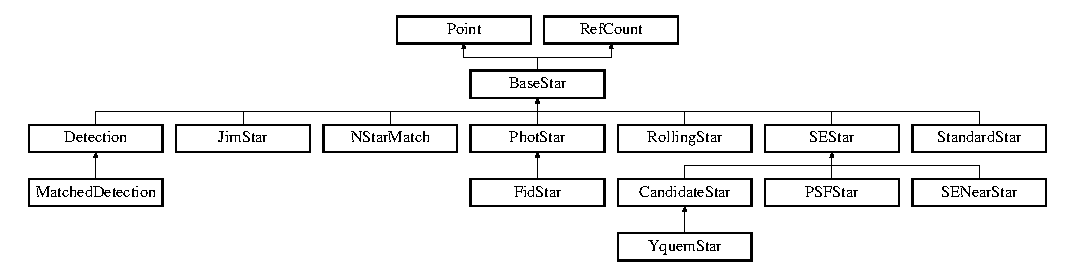
\includegraphics[height=3.27869cm]{class_basestar}
\end{center}
\end{figure}
\subsubsection*{Public Methods}
\begin{CompactItemize}
\item 
\index{BaseStar@{BaseStar}!BaseStar@{Base\-Star}}\index{BaseStar@{BaseStar}!BaseStar@{Base\-Star}}
{\bf Base\-Star} ()\label{class_basestar_a0}

\item 
\index{BaseStar@{BaseStar}!BaseStar@{Base\-Star}}\index{BaseStar@{BaseStar}!BaseStar@{Base\-Star}}
{\bf Base\-Star} (double xx, double yy, double ff)\label{class_basestar_a1}

\begin{CompactList}\small\item\em constructor.\item\end{CompactList}\item 
\index{BaseStar@{BaseStar}!BaseStar@{Base\-Star}}\index{BaseStar@{BaseStar}!BaseStar@{Base\-Star}}
{\bf Base\-Star} (const {\bf Point} \&a\_\-point, double a\_\-flux)\label{class_basestar_a2}

\item 
\index{X@{X}!BaseStar@{Base\-Star}}\index{BaseStar@{BaseStar}!X@{X}}
double {\bf X} () const\label{class_basestar_a3}

\begin{CompactList}\small\item\em access stuff.\item\end{CompactList}\item 
\index{Y@{Y}!BaseStar@{Base\-Star}}\index{BaseStar@{BaseStar}!Y@{Y}}
double {\bf Y} () const\label{class_basestar_a4}

\begin{CompactList}\small\item\em .\item\end{CompactList}\item 
\index{read_it@{read\_\-it}!BaseStar@{Base\-Star}}\index{BaseStar@{BaseStar}!read_it@{read\_\-it}}
void {\bf read\_\-it} (istream \&rd, const char $\ast$format)\label{class_basestar_a5}

\item 
\index{write@{write}!BaseStar@{Base\-Star}}\index{BaseStar@{BaseStar}!write@{write}}
virtual void {\bf write} (ostream \&s=cout) const\label{class_basestar_a6}

\item 
\index{writen@{writen}!BaseStar@{Base\-Star}}\index{BaseStar@{BaseStar}!writen@{writen}}
virtual void {\bf writen} (ostream \&s=cout) const\label{class_basestar_a7}

\item 
\index{dump@{dump}!BaseStar@{Base\-Star}}\index{BaseStar@{BaseStar}!dump@{dump}}
virtual void {\bf dump} (ostream \&stream=cout) const\label{class_basestar_a8}

\item 
\index{dumpn@{dumpn}!BaseStar@{Base\-Star}}\index{BaseStar@{BaseStar}!dumpn@{dumpn}}
virtual void {\bf dumpn} (ostream \&stream=cout) const\label{class_basestar_a9}

\item 
\index{operator=@{operator=}!BaseStar@{Base\-Star}}\index{BaseStar@{BaseStar}!operator=@{operator=}}
Base\-Star\& {\bf operator=} (const {\bf Point} \&P)\label{class_basestar_a10}

\item 
\index{~BaseStar@{$\sim$BaseStar}!BaseStar@{Base\-Star}}\index{BaseStar@{BaseStar}!~BaseStar@{$\sim$Base\-Star}}
virtual {\bf $\sim$Base\-Star} ()\label{class_basestar_a11}

\item 
\index{WriteHeader_@{WriteHeader\_\-}!BaseStar@{Base\-Star}}\index{BaseStar@{BaseStar}!WriteHeader_@{Write\-Header\_\-}}
virtual string {\bf Write\-Header\_\-} (ostream \&stream=cout, const char $\ast$i=NULL) const\label{class_basestar_a12}

\item 
\index{WriteHeader@{WriteHeader}!BaseStar@{Base\-Star}}\index{BaseStar@{BaseStar}!WriteHeader@{Write\-Header}}
virtual void {\bf Write\-Header} (ostream \&stream=cout) const\label{class_basestar_a13}

\end{CompactItemize}
\subsubsection*{Public Attributes}
\begin{CompactItemize}
\item 
\index{flux@{flux}!BaseStar@{Base\-Star}}\index{BaseStar@{BaseStar}!flux@{flux}}
double {\bf flux}\label{class_basestar_m0}

\end{CompactItemize}
\subsubsection*{Static Public Methods}
\begin{CompactItemize}
\item 
\index{read@{read}!BaseStar@{Base\-Star}}\index{BaseStar@{BaseStar}!read@{read}}
Base\-Star$\ast$ {\bf read} (istream \&rd, const char $\ast$format)\label{class_basestar_d0}

\item 
\index{TypeName@{TypeName}!BaseStar@{Base\-Star}}\index{BaseStar@{BaseStar}!TypeName@{Type\-Name}}
const char$\ast$ {\bf Type\-Name} ()\label{class_basestar_d1}

\end{CompactItemize}
\subsubsection*{Friends}
\begin{CompactItemize}
\item 
\index{operator<<@{operator$<$$<$}!BaseStar@{Base\-Star}}\index{BaseStar@{BaseStar}!operator<<@{operator$<$$<$}}
ostream\& {\bf operator$<$$<$} (ostream \&stream, const Base\-Star \&s)\label{class_basestar_l0}

\begin{CompactList}\small\item\em allows cout $<$$<$ a\-Base\-Star;.\item\end{CompactList}\end{CompactItemize}


\subsubsection{Detailed Description}
The base class for handling stars. Used by all matching routines.



The documentation for this class was generated from the following file:\begin{CompactItemize}
\item 
{\bf basestar.h}\end{CompactItemize}

\subsection{Component  Class Reference}
\label{class_component}\index{Component@{Component}}
store the necessary components for weighting and computing the stacking. 


{\tt \#include $<$imagesum.h$>$}

\subsubsection*{Public Methods}
\begin{CompactItemize}
\item 
\index{Component@{Component}!Component@{Component}}\index{Component@{Component}!Component@{Component}}
{\bf Component} ({\bf Reduced\-Image} $\ast$RI, const double \&Photom\-Ratio, const Weighting\-Method weighting\-Method)\label{class_component_a0}

\begin{CompactList}\small\item\em not to be stored.\item\end{CompactList}\item 
\index{dump@{dump}!Component@{Component}}\index{Component@{Component}!dump@{dump}}
void {\bf dump} (ostream \&s=cout) const\label{class_component_a1}

\item 
\index{~Component@{$\sim$Component}!Component@{Component}}\index{Component@{Component}!~Component@{$\sim$Component}}
{\bf $\sim$Component} ()\label{class_component_a2}

\end{CompactItemize}
\subsubsection*{Public Attributes}
\begin{CompactItemize}
\item 
\index{backVar@{backVar}!Component@{Component}}\index{Component@{Component}!backVar@{back\-Var}}
double {\bf back\-Var}\label{class_component_m0}

\item 
\index{seeing@{seeing}!Component@{Component}}\index{Component@{Component}!seeing@{seeing}}
double {\bf seeing}\label{class_component_m1}

\item 
\index{photomRatio@{photomRatio}!Component@{Component}}\index{Component@{Component}!photomRatio@{photom\-Ratio}}
double {\bf photom\-Ratio}\label{class_component_m2}

\item 
\index{globalWeight@{globalWeight}!Component@{Component}}\index{Component@{Component}!globalWeight@{global\-Weight}}
double {\bf global\-Weight}\label{class_component_m3}

\item 
\index{averageWeight@{averageWeight}!Component@{Component}}\index{Component@{Component}!averageWeight@{average\-Weight}}
double {\bf average\-Weight}\label{class_component_m4}

\item 
\index{hasWeight@{hasWeight}!Component@{Component}}\index{Component@{Component}!hasWeight@{has\-Weight}}
bool {\bf has\-Weight}\label{class_component_m5}

\item 
\index{hasDead@{hasDead}!Component@{Component}}\index{Component@{Component}!hasDead@{has\-Dead}}
bool {\bf has\-Dead}\label{class_component_m6}

\item 
\index{hasSatur@{hasSatur}!Component@{Component}}\index{Component@{Component}!hasSatur@{has\-Satur}}
bool {\bf has\-Satur}\label{class_component_m7}

\item 
\index{hasCosmic@{hasCosmic}!Component@{Component}}\index{Component@{Component}!hasCosmic@{has\-Cosmic}}
bool {\bf has\-Cosmic}\label{class_component_m8}

\item 
\index{reducedImageName@{reducedImageName}!Component@{Component}}\index{Component@{Component}!reducedImageName@{reduced\-Image\-Name}}
string {\bf reduced\-Image\-Name}\label{class_component_m9}

\item 
\index{Ri@{Ri}!Component@{Component}}\index{Component@{Component}!Ri@{Ri}}
Reduced\-Image\-Ref {\bf Ri}\label{class_component_m10}

\end{CompactItemize}


\subsubsection{Detailed Description}
store the necessary components for weighting and computing the stacking.



The documentation for this class was generated from the following file:\begin{CompactItemize}
\item 
{\bf imagesum.h}\end{CompactItemize}

\subsection{Counted\-Ref  Class Template Reference}
\label{class_countedref}\index{CountedRef@{Counted\-Ref}}
an implementation of \char`\"{}smart pointers\char`\"{} that counts references to an object. The obejct it \char`\"{}points\char`\"{} to has to derive from Ref\-Count. 


{\tt \#include $<$countedref.h$>$}

Inheritance diagram for Counted\-Ref::\begin{figure}[H]
\begin{center}
\leavevmode
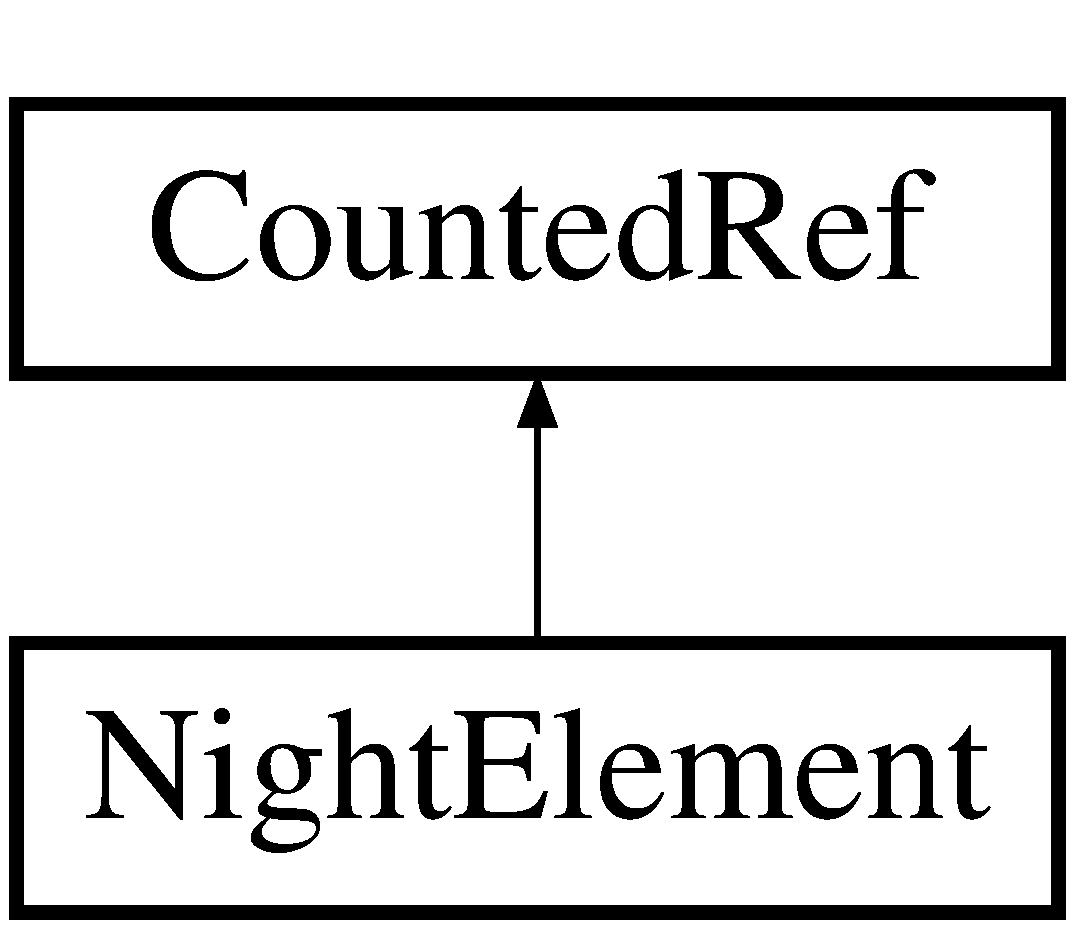
\includegraphics[height=2cm]{class_countedref}
\end{center}
\end{figure}
\subsubsection*{Public Methods}
\begin{CompactItemize}
\item 
\index{CountedRef@{CountedRef}!CountedRef@{Counted\-Ref}}\index{CountedRef@{CountedRef}!CountedRef@{Counted\-Ref}}
{\bf Counted\-Ref} ()\label{class_countedref_a0}

\item 
\index{CountedRef@{CountedRef}!CountedRef@{Counted\-Ref}}\index{CountedRef@{CountedRef}!CountedRef@{Counted\-Ref}}
{\bf Counted\-Ref} (T $\ast$pp)\label{class_countedref_a1}

\item 
\index{CountedRef@{CountedRef}!CountedRef@{Counted\-Ref}}\index{CountedRef@{CountedRef}!CountedRef@{Counted\-Ref}}
{\bf Counted\-Ref} (const T $\ast$pp)\label{class_countedref_a2}

\item 
\index{operator=@{operator=}!CountedRef@{Counted\-Ref}}\index{CountedRef@{CountedRef}!operator=@{operator=}}
void {\bf operator=} (const Counted\-Ref \&Right)\label{class_countedref_a3}

\item 
\index{CountedRef@{CountedRef}!CountedRef@{Counted\-Ref}}\index{CountedRef@{CountedRef}!CountedRef@{Counted\-Ref}}
{\bf Counted\-Ref} (const Counted\-Ref \&Other)\label{class_countedref_a4}

\item 
\index{operator const T *@{operator const T $\ast$}!CountedRef@{Counted\-Ref}}\index{CountedRef@{CountedRef}!operator const T *@{operator const T $\ast$}}
{\bf operator const T $\ast$} () const\label{class_countedref_a5}

\item 
\index{operator T *@{operator T $\ast$}!CountedRef@{Counted\-Ref}}\index{CountedRef@{CountedRef}!operator T *@{operator T $\ast$}}
{\bf operator T $\ast$} ()\label{class_countedref_a6}

\item 
\index{operator->@{operator-$>$}!CountedRef@{Counted\-Ref}}\index{CountedRef@{CountedRef}!operator->@{operator $\rightarrow$ }}
T$\ast$ {\bf operator $\rightarrow$ } ()\label{class_countedref_a7}

\item 
\index{operator->@{operator-$>$}!CountedRef@{Counted\-Ref}}\index{CountedRef@{CountedRef}!operator->@{operator $\rightarrow$ }}
const T$\ast$ {\bf operator $\rightarrow$ } () const\label{class_countedref_a8}

\item 
\index{operator *@{operator $\ast$}!CountedRef@{Counted\-Ref}}\index{CountedRef@{CountedRef}!operator *@{operator $\ast$}}
T\& {\bf operator $\ast$} ()\label{class_countedref_a9}

\item 
\index{operator *@{operator $\ast$}!CountedRef@{Counted\-Ref}}\index{CountedRef@{CountedRef}!operator *@{operator $\ast$}}
const T\& {\bf operator $\ast$} () const\label{class_countedref_a10}

\item 
\index{operator==@{operator==}!CountedRef@{Counted\-Ref}}\index{CountedRef@{CountedRef}!operator==@{operator==}}
bool {\bf operator==} (const Counted\-Ref$<$ T $>$ \&Right) const\label{class_countedref_a11}

\item 
\index{operator==@{operator==}!CountedRef@{Counted\-Ref}}\index{CountedRef@{CountedRef}!operator==@{operator==}}
bool {\bf operator==} (const T $\ast$Right) const\label{class_countedref_a12}

\item 
\index{operator"!=@{operator"!=}!CountedRef@{Counted\-Ref}}\index{CountedRef@{CountedRef}!operator!=@{operator!=}}
bool {\bf operator!=} (const Counted\-Ref$<$ T $>$ \&Right) const\label{class_countedref_a13}

\item 
\index{operator"!=@{operator"!=}!CountedRef@{Counted\-Ref}}\index{CountedRef@{CountedRef}!operator!=@{operator!=}}
bool {\bf operator!=} (const T $\ast$Right) const\label{class_countedref_a14}

\item 
\index{operator A *@{operator A $\ast$}!CountedRef@{Counted\-Ref}}\index{CountedRef@{CountedRef}!operator A *@{operator A $\ast$}}
template$<$class A$>$ {\bf operator A $\ast$} ()\label{class_countedref_a15}

\item 
\index{operator const A *@{operator const A $\ast$}!CountedRef@{Counted\-Ref}}\index{CountedRef@{CountedRef}!operator const A *@{operator const A $\ast$}}
template$<$class A$>$ {\bf operator const A $\ast$} () const\label{class_countedref_a16}

\item 
\index{~CountedRef@{$\sim$CountedRef}!CountedRef@{Counted\-Ref}}\index{CountedRef@{CountedRef}!~CountedRef@{$\sim$Counted\-Ref}}
{\bf $\sim$Counted\-Ref} ()\label{class_countedref_a17}

\end{CompactItemize}


\subsubsection{Detailed Description}
\subsubsection*{template$<$class T$>$  class Counted\-Ref}

an implementation of \char`\"{}smart pointers\char`\"{} that counts references to an object. The obejct it \char`\"{}points\char`\"{} to has to derive from Ref\-Count.



The documentation for this class was generated from the following file:\begin{CompactItemize}
\item 
{\bf countedref.h}\end{CompactItemize}

\subsection{Daophot  Class Reference}
\label{class_daophot}\index{Daophot@{Daophot}}
a wrapper to most DAOPHOT routines. 


{\tt \#include $<$daophot.h$>$}

\subsubsection*{Public Methods}
\begin{CompactItemize}
\item 
\index{Daophot@{Daophot}!Daophot@{Daophot}}\index{Daophot@{Daophot}!Daophot@{Daophot}}
{\bf Daophot} ()\label{class_daophot_a0}

\item 
\index{Daophot@{Daophot}!Daophot@{Daophot}}\index{Daophot@{Daophot}!Daophot@{Daophot}}
{\bf Daophot} (const string \&Fits\-Name)\label{class_daophot_a1}

\item 
\index{Daophot@{Daophot}!Daophot@{Daophot}}\index{Daophot@{Daophot}!Daophot@{Daophot}}
{\bf Daophot} (const {\bf Reduced\-Image} \&Rim)\label{class_daophot_a2}

\item 
\index{~Daophot@{$\sim$Daophot}!Daophot@{Daophot}}\index{Daophot@{Daophot}!~Daophot@{$\sim$Daophot}}
{\bf $\sim$Daophot} ()\label{class_daophot_a3}

\item 
\index{WriteOptions@{WriteOptions}!Daophot@{Daophot}}\index{Daophot@{Daophot}!WriteOptions@{Write\-Options}}
void {\bf Write\-Options} (const string File\-Name=\char`\"{}daophot.opt\char`\"{}, const int First=0, const int Last=NOPT-1) const\label{class_daophot_a4}

\item 
\index{Option@{Option}!Daophot@{Daophot}}\index{Daophot@{Daophot}!Option@{Option}}
void {\bf Option} (const string Opt\-File=\char`\"{}daophot.opt\char`\"{}) const\label{class_daophot_a5}

\item 
\index{SetOptions@{SetOptions}!Daophot@{Daophot}}\index{Daophot@{Daophot}!SetOptions@{Set\-Options}}
void {\bf Set\-Options} (const {\bf Reduced\-Image} \&Rim)\label{class_daophot_a6}

\item 
\index{AddStars@{AddStars}!Daophot@{Daophot}}\index{Daophot@{Daophot}!AddStars@{Add\-Stars}}
void {\bf Add\-Stars} ()\label{class_daophot_a7}

\item 
\index{AllStar@{AllStar}!Daophot@{Daophot}}\index{Daophot@{Daophot}!AllStar@{All\-Star}}
void {\bf All\-Star} (const string \&File\-With\-Stars\-To\-Fit) const\label{class_daophot_a8}

\item 
\index{Attach@{Attach}!Daophot@{Daophot}}\index{Daophot@{Daophot}!Attach@{Attach}}
void {\bf Attach} (const string Fits\-Name)\label{class_daophot_a9}

\item 
\index{Find@{Find}!Daophot@{Daophot}}\index{Daophot@{Daophot}!Find@{Find}}
void {\bf Find} () const\label{class_daophot_a10}

\item 
\index{Group@{Group}!Daophot@{Daophot}}\index{Daophot@{Daophot}!Group@{Group}}
void {\bf Group} () const\label{class_daophot_a11}

\item 
\index{Nstar@{Nstar}!Daophot@{Daophot}}\index{Daophot@{Daophot}!Nstar@{Nstar}}
void {\bf Nstar} () const\label{class_daophot_a12}

\item 
\index{Peak@{Peak}!Daophot@{Daophot}}\index{Daophot@{Daophot}!Peak@{Peak}}
void {\bf Peak} () const\label{class_daophot_a13}

\item 
\index{PeakFit@{PeakFit}!Daophot@{Daophot}}\index{Daophot@{Daophot}!PeakFit@{Peak\-Fit}}
void {\bf Peak\-Fit} ({\bf SEStar} \&Star) const\label{class_daophot_a14}

\item 
\index{Pick@{Pick}!Daophot@{Daophot}}\index{Daophot@{Daophot}!Pick@{Pick}}
void {\bf Pick} () const\label{class_daophot_a15}

\item 
\index{Photometry@{Photometry}!Daophot@{Daophot}}\index{Daophot@{Daophot}!Photometry@{Photometry}}
void {\bf Photometry} () const\label{class_daophot_a16}

\item 
\index{Psf@{Psf}!Daophot@{Daophot}}\index{Daophot@{Daophot}!Psf@{Psf}}
void {\bf Psf} (const int Variability=0, const bool Manual=false)\label{class_daophot_a17}

\item 
\index{Sky@{Sky}!Daophot@{Daophot}}\index{Daophot@{Daophot}!Sky@{Sky}}
void {\bf Sky} (float \&Sky\-Mean, float \&Sky\-Median, float \&Sky\-Mode, float \&Sky\-Sigma) const\label{class_daophot_a18}

\item 
\index{SubStar@{SubStar}!Daophot@{Daophot}}\index{Daophot@{Daophot}!SubStar@{Sub\-Star}}
void {\bf Sub\-Star} () const\label{class_daophot_a19}

\item 
\index{IterPsf@{IterPsf}!Daophot@{Daophot}}\index{Daophot@{Daophot}!IterPsf@{Iter\-Psf}}
void {\bf Iter\-Psf} (const {\bf Reduced\-Image} \&Rim, const bool Manual=false)\label{class_daophot_a20}

\item 
\index{PrecisePsf@{PrecisePsf}!Daophot@{Daophot}}\index{Daophot@{Daophot}!PrecisePsf@{Precise\-Psf}}
void {\bf Precise\-Psf} (const {\bf Reduced\-Image} \&Rim)\label{class_daophot_a21}

\end{CompactItemize}


\subsubsection{Detailed Description}
a wrapper to most DAOPHOT routines.



The documentation for this class was generated from the following file:\begin{CompactItemize}
\item 
{\bf daophot.h}\end{CompactItemize}

\subsection{Db\-Image  Class Reference}
\label{class_dbimage}\index{DbImage@{Db\-Image}}
{\tt \#include $<$dbimage.h$>$}

Inheritance diagram for Db\-Image::\begin{figure}[H]
\begin{center}
\leavevmode
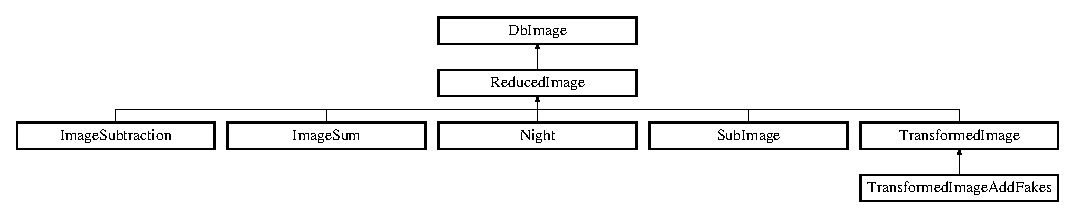
\includegraphics[height=2.47514cm]{class_dbimage}
\end{center}
\end{figure}
\subsubsection*{Public Methods}
\begin{CompactItemize}
\item 
\index{DbImage@{DbImage}!DbImage@{Db\-Image}}\index{DbImage@{DbImage}!DbImage@{Db\-Image}}
{\bf Db\-Image} (const string \&Image\-Name)\label{class_dbimage_a0}

\begin{CompactList}\small\item\em a constructor: its argument is a unique image identifier (eg r124280).\item\end{CompactList}\item 
\index{DbImage@{DbImage}!DbImage@{Db\-Image}}\index{DbImage@{DbImage}!DbImage@{Db\-Image}}
{\bf Db\-Image} (const char $\ast$Image\-Name)\label{class_dbimage_a1}

\begin{CompactList}\small\item\em a constructor: its argument is a unique image identifier (eg r124280).\item\end{CompactList}\item 
\index{DbImage@{DbImage}!DbImage@{Db\-Image}}\index{DbImage@{DbImage}!DbImage@{Db\-Image}}
{\bf Db\-Image} ()\label{class_dbimage_a2}

\item 
\index{IsValid@{IsValid}!DbImage@{Db\-Image}}\index{DbImage@{DbImage}!IsValid@{Is\-Valid}}
bool {\bf Is\-Valid} () const\label{class_dbimage_a3}

\begin{CompactList}\small\item\em for images obtained from the above constructor, checks that the image could be located.\item\end{CompactList}\item 
\index{Name@{Name}!DbImage@{Db\-Image}}\index{DbImage@{DbImage}!Name@{Name}}
string {\bf Name} () const\label{class_dbimage_a4}

\begin{CompactList}\small\item\em returns the image name.\item\end{CompactList}\item 
\index{Dir@{Dir}!DbImage@{Db\-Image}}\index{DbImage@{DbImage}!Dir@{Dir}}
string {\bf Dir} () const\label{class_dbimage_a5}

\item 
\index{DbImage@{DbImage}!DbImage@{Db\-Image}}\index{DbImage@{DbImage}!DbImage@{Db\-Image}}
{\bf Db\-Image} (const string \&Image\-Name, const Path $\ast$APath)\label{class_dbimage_a6}

\item 
\index{operator==@{operator==}!DbImage@{Db\-Image}}\index{DbImage@{DbImage}!operator==@{operator==}}
bool {\bf operator==} (const Db\-Image \&Right) const\label{class_dbimage_a7}

\begin{CompactList}\small\item\em to tell if we have twice the same image.\item\end{CompactList}\item 
string {\bf Fits\-Image\-Name} (const Db\-Image\-Kind Kind) const
\begin{CompactList}\small\item\em returns the {\bf Fits\-Image} {\rm (p.\,\pageref{class_fitsimage})} file name (a file name for the file system).\item\end{CompactList}\item 
\index{ElixirName@{ElixirName}!DbImage@{Db\-Image}}\index{DbImage@{DbImage}!ElixirName@{Elixir\-Name}}
string {\bf Elixir\-Name} () const\label{class_dbimage_a9}

\begin{CompactList}\small\item\em out of elixir name.\item\end{CompactList}\item 
string {\bf Image\-Back\-Name} (const Db\-Image\-Kind Kind) const
\begin{CompactList}\small\item\em same for the {\bf Image\-Back} {\rm (p.\,\pageref{class_imageback})} (background value and rms interpolated map).\item\end{CompactList}\item 
\index{FitsFlatName@{FitsFlatName}!DbImage@{Db\-Image}}\index{DbImage@{DbImage}!FitsFlatName@{Fits\-Flat\-Name}}
string {\bf Fits\-Flat\-Name} () const\label{class_dbimage_a11}

\begin{CompactList}\small\item\em the name of the fits file containig the flatfield used for flatfielding.\item\end{CompactList}\item 
\index{FitsBiasName@{FitsBiasName}!DbImage@{Db\-Image}}\index{DbImage@{DbImage}!FitsBiasName@{Fits\-Bias\-Name}}
string {\bf Fits\-Bias\-Name} () const\label{class_dbimage_a12}

\begin{CompactList}\small\item\em same for bias.\item\end{CompactList}\item 
\index{FitsDarkName@{FitsDarkName}!DbImage@{Db\-Image}}\index{DbImage@{DbImage}!FitsDarkName@{Fits\-Dark\-Name}}
string {\bf Fits\-Dark\-Name} () const\label{class_dbimage_a13}

\begin{CompactList}\small\item\em same for dark.\item\end{CompactList}\item 
\index{FitsWeightName@{FitsWeightName}!DbImage@{Db\-Image}}\index{DbImage@{DbImage}!FitsWeightName@{Fits\-Weight\-Name}}
string {\bf Fits\-Weight\-Name} () const\label{class_dbimage_a14}

\begin{CompactList}\small\item\em name of the weight imag.\item\end{CompactList}\item 
\index{FitsDeadName@{FitsDeadName}!DbImage@{Db\-Image}}\index{DbImage@{DbImage}!FitsDeadName@{Fits\-Dead\-Name}}
string {\bf Fits\-Dead\-Name} () const\label{class_dbimage_a15}

\begin{CompactList}\small\item\em same for dead pixel map.\item\end{CompactList}\item 
\index{FitsBadName@{FitsBadName}!DbImage@{Db\-Image}}\index{DbImage@{DbImage}!FitsBadName@{Fits\-Bad\-Name}}
string {\bf Fits\-Bad\-Name} () const\label{class_dbimage_a16}

\begin{CompactList}\small\item\em same for bad pixel map (built from weight map).\item\end{CompactList}\item 
\index{FitsCosmicName@{FitsCosmicName}!DbImage@{Db\-Image}}\index{DbImage@{DbImage}!FitsCosmicName@{Fits\-Cosmic\-Name}}
string {\bf Fits\-Cosmic\-Name} () const\label{class_dbimage_a17}

\begin{CompactList}\small\item\em same for cosmic pixel map.\item\end{CompactList}\item 
\index{FitsSatelliteName@{FitsSatelliteName}!DbImage@{Db\-Image}}\index{DbImage@{DbImage}!FitsSatelliteName@{Fits\-Satellite\-Name}}
string {\bf Fits\-Satellite\-Name} () const\label{class_dbimage_a18}

\begin{CompactList}\small\item\em same for satellite pixel map.\item\end{CompactList}\item 
\index{FitsFringeName@{FitsFringeName}!DbImage@{Db\-Image}}\index{DbImage@{DbImage}!FitsFringeName@{Fits\-Fringe\-Name}}
string {\bf Fits\-Fringe\-Name} () const\label{class_dbimage_a19}

\begin{CompactList}\small\item\em same for fringe pattern map map.\item\end{CompactList}\item 
\index{FitsBackName@{FitsBackName}!DbImage@{Db\-Image}}\index{DbImage@{DbImage}!FitsBackName@{Fits\-Back\-Name}}
string {\bf Fits\-Back\-Name} () const\label{class_dbimage_a20}

\begin{CompactList}\small\item\em background image.\item\end{CompactList}\item 
\index{FitsMiniBackName@{FitsMiniBackName}!DbImage@{Db\-Image}}\index{DbImage@{DbImage}!FitsMiniBackName@{Fits\-Mini\-Back\-Name}}
string {\bf Fits\-Mini\-Back\-Name} () const\label{class_dbimage_a21}

\begin{CompactList}\small\item\em min background image.\item\end{CompactList}\item 
\index{FitsSaturName@{FitsSaturName}!DbImage@{Db\-Image}}\index{DbImage@{DbImage}!FitsSaturName@{Fits\-Satur\-Name}}
string {\bf Fits\-Satur\-Name} () const\label{class_dbimage_a22}

\begin{CompactList}\small\item\em same for saturated stars pixels map.\item\end{CompactList}\item 
\index{ImageMatchUsnoName@{ImageMatchUsnoName}!DbImage@{Db\-Image}}\index{DbImage@{DbImage}!ImageMatchUsnoName@{Image\-Match\-Usno\-Name}}
string {\bf Image\-Match\-Usno\-Name} () const\label{class_dbimage_a23}

\begin{CompactList}\small\item\em return the results of the usno match.\item\end{CompactList}\item 
string {\bf Image\-Catalog\-Name} (const Db\-Image\-Catalog\-Kind Kind=SExtractor) const
\begin{CompactList}\small\item\em returns the list of stars detected and measured on the {\bf Image} {\rm (p.\,\pageref{class_image})} (a file name for the file system).\item\end{CompactList}\item 
\index{ImagePsfName@{ImagePsfName}!DbImage@{Db\-Image}}\index{DbImage@{DbImage}!ImagePsfName@{Image\-Psf\-Name}}
string {\bf Image\-Psf\-Name} (const Db\-Image\-Psf\-Kind Kind=Daophot\-Psf) const\label{class_dbimage_a25}

\begin{CompactList}\small\item\em returns the name where the psf parameters and look-up table for residuals is stored.\item\end{CompactList}\item 
\index{EverythingElseFileName@{EverythingElseFileName}!DbImage@{Db\-Image}}\index{DbImage@{DbImage}!EverythingElseFileName@{Everything\-Else\-File\-Name}}
string {\bf Everything\-Else\-File\-Name} () const\label{class_dbimage_a26}

\item 
\index{Create@{Create}!DbImage@{Db\-Image}}\index{DbImage@{DbImage}!Create@{Create}}
bool {\bf Create} (const string \&Path)\label{class_dbimage_a27}

\begin{CompactList}\small\item\em To create the directories where the fits images, catalogues will be put: ex: $\sim$/Fake\-Db/test: Db\-Image dbim(\char`\"{}test\char`\"{}); dbim.Create(\char`\"{}$\sim$/Fake\-Db/\char`\"{});.\item\end{CompactList}\item 
\index{GetFileName@{GetFileName}!DbImage@{Db\-Image}}\index{DbImage@{DbImage}!GetFileName@{Get\-File\-Name}}
string {\bf Get\-File\-Name} (const char $\ast$Which\-File) const\label{class_dbimage_a28}

\item 
\index{dump@{dump}!DbImage@{Db\-Image}}\index{DbImage@{DbImage}!dump@{dump}}
void {\bf dump} (ostream \&stream=cout) const\label{class_dbimage_a29}

\item 
\index{~DbImage@{$\sim$DbImage}!DbImage@{Db\-Image}}\index{DbImage@{DbImage}!~DbImage@{$\sim$Db\-Image}}
{\bf $\sim$Db\-Image} ()\label{class_dbimage_a30}

\item 
\index{init_from_name@{init\_\-from\_\-name}!DbImage@{Db\-Image}}\index{DbImage@{DbImage}!init_from_name@{init\_\-from\_\-name}}
void {\bf init\_\-from\_\-name} ()\label{class_dbimage_a31}

\item 
\index{writeEverythingElse@{writeEverythingElse}!DbImage@{Db\-Image}}\index{DbImage@{DbImage}!writeEverythingElse@{write\-Everything\-Else}}
bool {\bf write\-Everything\-Else} ()\label{class_dbimage_a32}

\end{CompactItemize}
\subsubsection*{Protected Attributes}
\begin{CompactItemize}
\item 
\index{saveEverythingElse@{saveEverythingElse}!DbImage@{Db\-Image}}\index{DbImage@{DbImage}!saveEverythingElse@{save\-Everything\-Else}}
bool {\bf save\-Everything\-Else}\label{class_dbimage_n0}

\end{CompactItemize}
\subsubsection*{Friends}
\begin{CompactItemize}
\item 
class {\bf Db\-Image\-List}
\item 
class {\bf operator$<$$<$}
\end{CompactItemize}


\subsubsection{Detailed Description}
A Db\-Image refers to one image as the telescope provides it (more precisely, one CCD), together with associated data used for the reduction (flat and bias frames) or produced  during the reduction (lists of stars). 



\subsubsection{Member Function Documentation}
\index{DbImage@{Db\-Image}!FitsImageName@{FitsImageName}}
\index{FitsImageName@{FitsImageName}!DbImage@{Db\-Image}}
\paragraph{\setlength{\rightskip}{0pt plus 5cm}string Db\-Image::Fits\-Image\-Name (const Db\-Image\-Kind {\em Kind}) const}\hfill\label{class_dbimage_a8}


returns the {\bf Fits\-Image} {\rm (p.\,\pageref{class_fitsimage})} file name (a file name for the file system).

The Kind argument can be Raw or Flat\-Fielded. Nothing ensures that the file exists. One may use the File\-Exists routine  to check. \index{DbImage@{Db\-Image}!ImageBackName@{ImageBackName}}
\index{ImageBackName@{ImageBackName}!DbImage@{Db\-Image}}
\paragraph{\setlength{\rightskip}{0pt plus 5cm}string Db\-Image::Image\-Back\-Name (const Db\-Image\-Kind {\em Kind}) const}\hfill\label{class_dbimage_a10}


same for the {\bf Image\-Back} {\rm (p.\,\pageref{class_imageback})} (background value and rms interpolated map).

Same remark as above concerning the existence. \index{DbImage@{Db\-Image}!ImageCatalogName@{ImageCatalogName}}
\index{ImageCatalogName@{ImageCatalogName}!DbImage@{Db\-Image}}
\paragraph{\setlength{\rightskip}{0pt plus 5cm}string Db\-Image::Image\-Catalog\-Name (const Db\-Image\-Catalog\-Kind {\em Kind} = SExtractor) const}\hfill\label{class_dbimage_a24}


returns the list of stars detected and measured on the {\bf Image} {\rm (p.\,\pageref{class_image})} (a file name for the file system).

The Kind argument can be SExtractor or Fitted\_\-for\_\-seeing.  See Fits\-Image\-Name for caution instructions 

The documentation for this class was generated from the following file:\begin{CompactItemize}
\item 
{\bf dbimage.h}\end{CompactItemize}

\subsection{Db\-Image\-List  Class Reference}
\label{class_dbimagelist}\index{DbImageList@{Db\-Image\-List}}
Db\-Images can be globally located and stored into image lists. 


{\tt \#include $<$dbimage.h$>$}

Inheritance diagram for Db\-Image\-List::\begin{figure}[H]
\begin{center}
\leavevmode
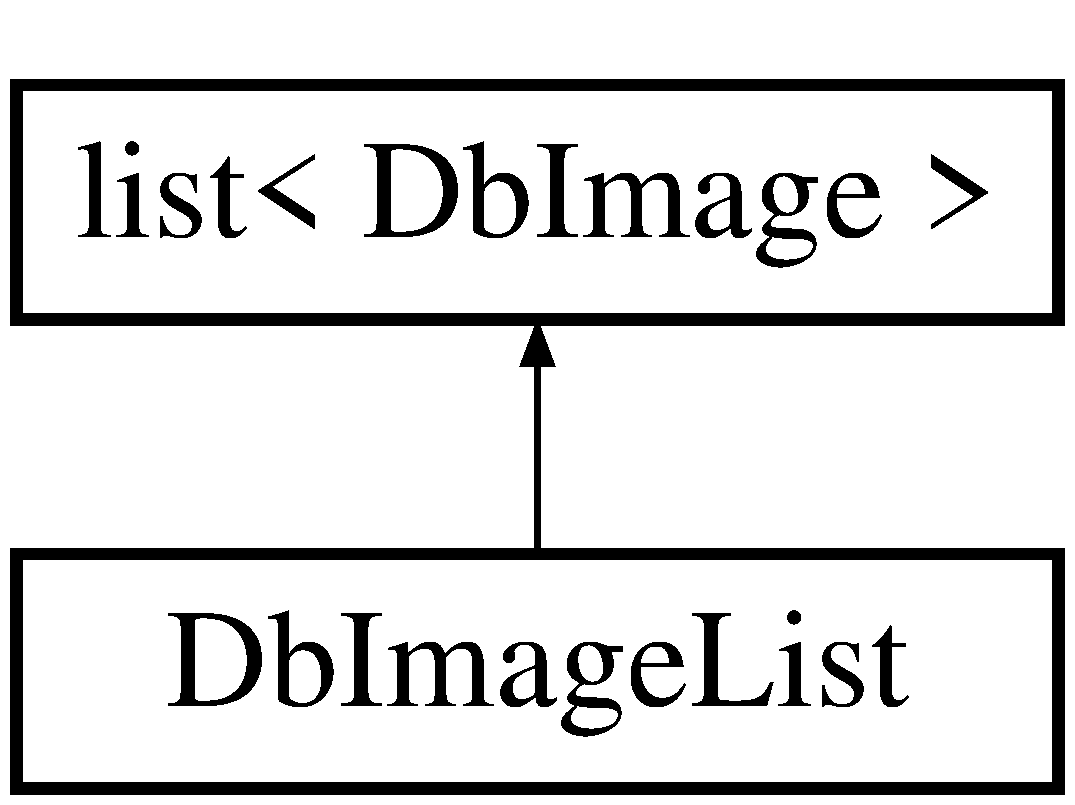
\includegraphics[height=2cm]{class_dbimagelist}
\end{center}
\end{figure}
\subsubsection*{Public Methods}
\begin{CompactItemize}
\item 
{\bf Db\-Image\-List} (const char $\ast$Path\-Name)
\begin{CompactList}\small\item\em locates all {\bf Db\-Image} {\rm (p.\,\pageref{class_dbimage})}'s in a given symbolic path name (see db configuration file section).\item\end{CompactList}\item 
\index{DbImageList@{DbImageList}!DbImageList@{Db\-Image\-List}}\index{DbImageList@{DbImageList}!DbImageList@{Db\-Image\-List}}
{\bf Db\-Image\-List} (const string \&Path\-Name)\label{class_dbimagelist_a1}

\item 
\index{DbImageList@{DbImageList}!DbImageList@{Db\-Image\-List}}\index{DbImageList@{DbImageList}!DbImageList@{Db\-Image\-List}}
{\bf Db\-Image\-List} (const list$<$ string $>$ names)\label{class_dbimagelist_a2}

\begin{CompactList}\small\item\em tries to interpret ecah argument either as a {\bf Db\-Image} {\rm (p.\,\pageref{class_dbimage})} name or as a symbolic path.\item\end{CompactList}\item 
\index{DbImageList@{DbImageList}!DbImageList@{Db\-Image\-List}}\index{DbImageList@{DbImageList}!DbImageList@{Db\-Image\-List}}
{\bf Db\-Image\-List} ()\label{class_dbimagelist_a3}

\item 
\index{FilterByDate@{FilterByDate}!DbImageList@{Db\-Image\-List}}\index{DbImageList@{DbImageList}!FilterByDate@{Filter\-By\-Date}}
void {\bf Filter\-By\-Date} (const int a\_\-date)\label{class_dbimagelist_a4}

\begin{CompactList}\small\item\em discards from a Db\-Image\-List all images not matching a date.\item\end{CompactList}\item 
\index{Collect@{Collect}!DbImageList@{Db\-Image\-List}}\index{DbImageList@{DbImageList}!Collect@{Collect}}
int {\bf Collect} (const char $\ast$Path\-Name)\label{class_dbimagelist_a5}

\begin{CompactList}\small\item\em DOCF collects and appends Db\-Images inside Path\-Name.\item\end{CompactList}\item 
\index{dump@{dump}!DbImageList@{Db\-Image\-List}}\index{DbImageList@{DbImageList}!dump@{dump}}
void {\bf dump} (ostream \&stream=cout) const\label{class_dbimagelist_a6}

\end{CompactItemize}
\subsubsection*{Friends}
\begin{CompactItemize}
\item 
\index{operator<<@{operator$<$$<$}!DbImageList@{Db\-Image\-List}}\index{DbImageList@{DbImageList}!operator<<@{operator$<$$<$}}
ostream\& {\bf operator$<$$<$} (ostream \&stream, const Db\-Image\-List \&L)\label{class_dbimagelist_l0}

\begin{CompactList}\small\item\em example of usage : cout $<$$<$ Db\-Image\-List(\char`\"{}$\ast$\char`\"{}); . It works as the first statement of your program !\item\end{CompactList}\end{CompactItemize}


\subsubsection{Detailed Description}
Db\-Images can be globally located and stored into image lists.



\subsubsection{Constructor \& Destructor Documentation}
\index{DbImageList@{Db\-Image\-List}!DbImageList@{DbImageList}}
\index{DbImageList@{DbImageList}!DbImageList@{Db\-Image\-List}}
\paragraph{\setlength{\rightskip}{0pt plus 5cm}Db\-Image\-List::Db\-Image\-List (const char $\ast$ {\em Path\-Name})}\hfill\label{class_dbimagelist_a0}


locates all {\bf Db\-Image} {\rm (p.\,\pageref{class_dbimage})}'s in a given symbolic path name (see db configuration file section).

This routine handles wildcards : $\ast$ will match any path name, 'new$\ast$' will match any path name beginning with 'new'. 

The documentation for this class was generated from the following file:\begin{CompactItemize}
\item 
{\bf dbimage.h}\end{CompactItemize}

\subsection{DImage  Class Reference}
\label{class_dimage}\index{DImage@{DImage}}
a double precision image type. 


{\tt \#include $<$dimage.h$>$}

Inheritance diagram for DImage::\begin{figure}[H]
\begin{center}
\leavevmode
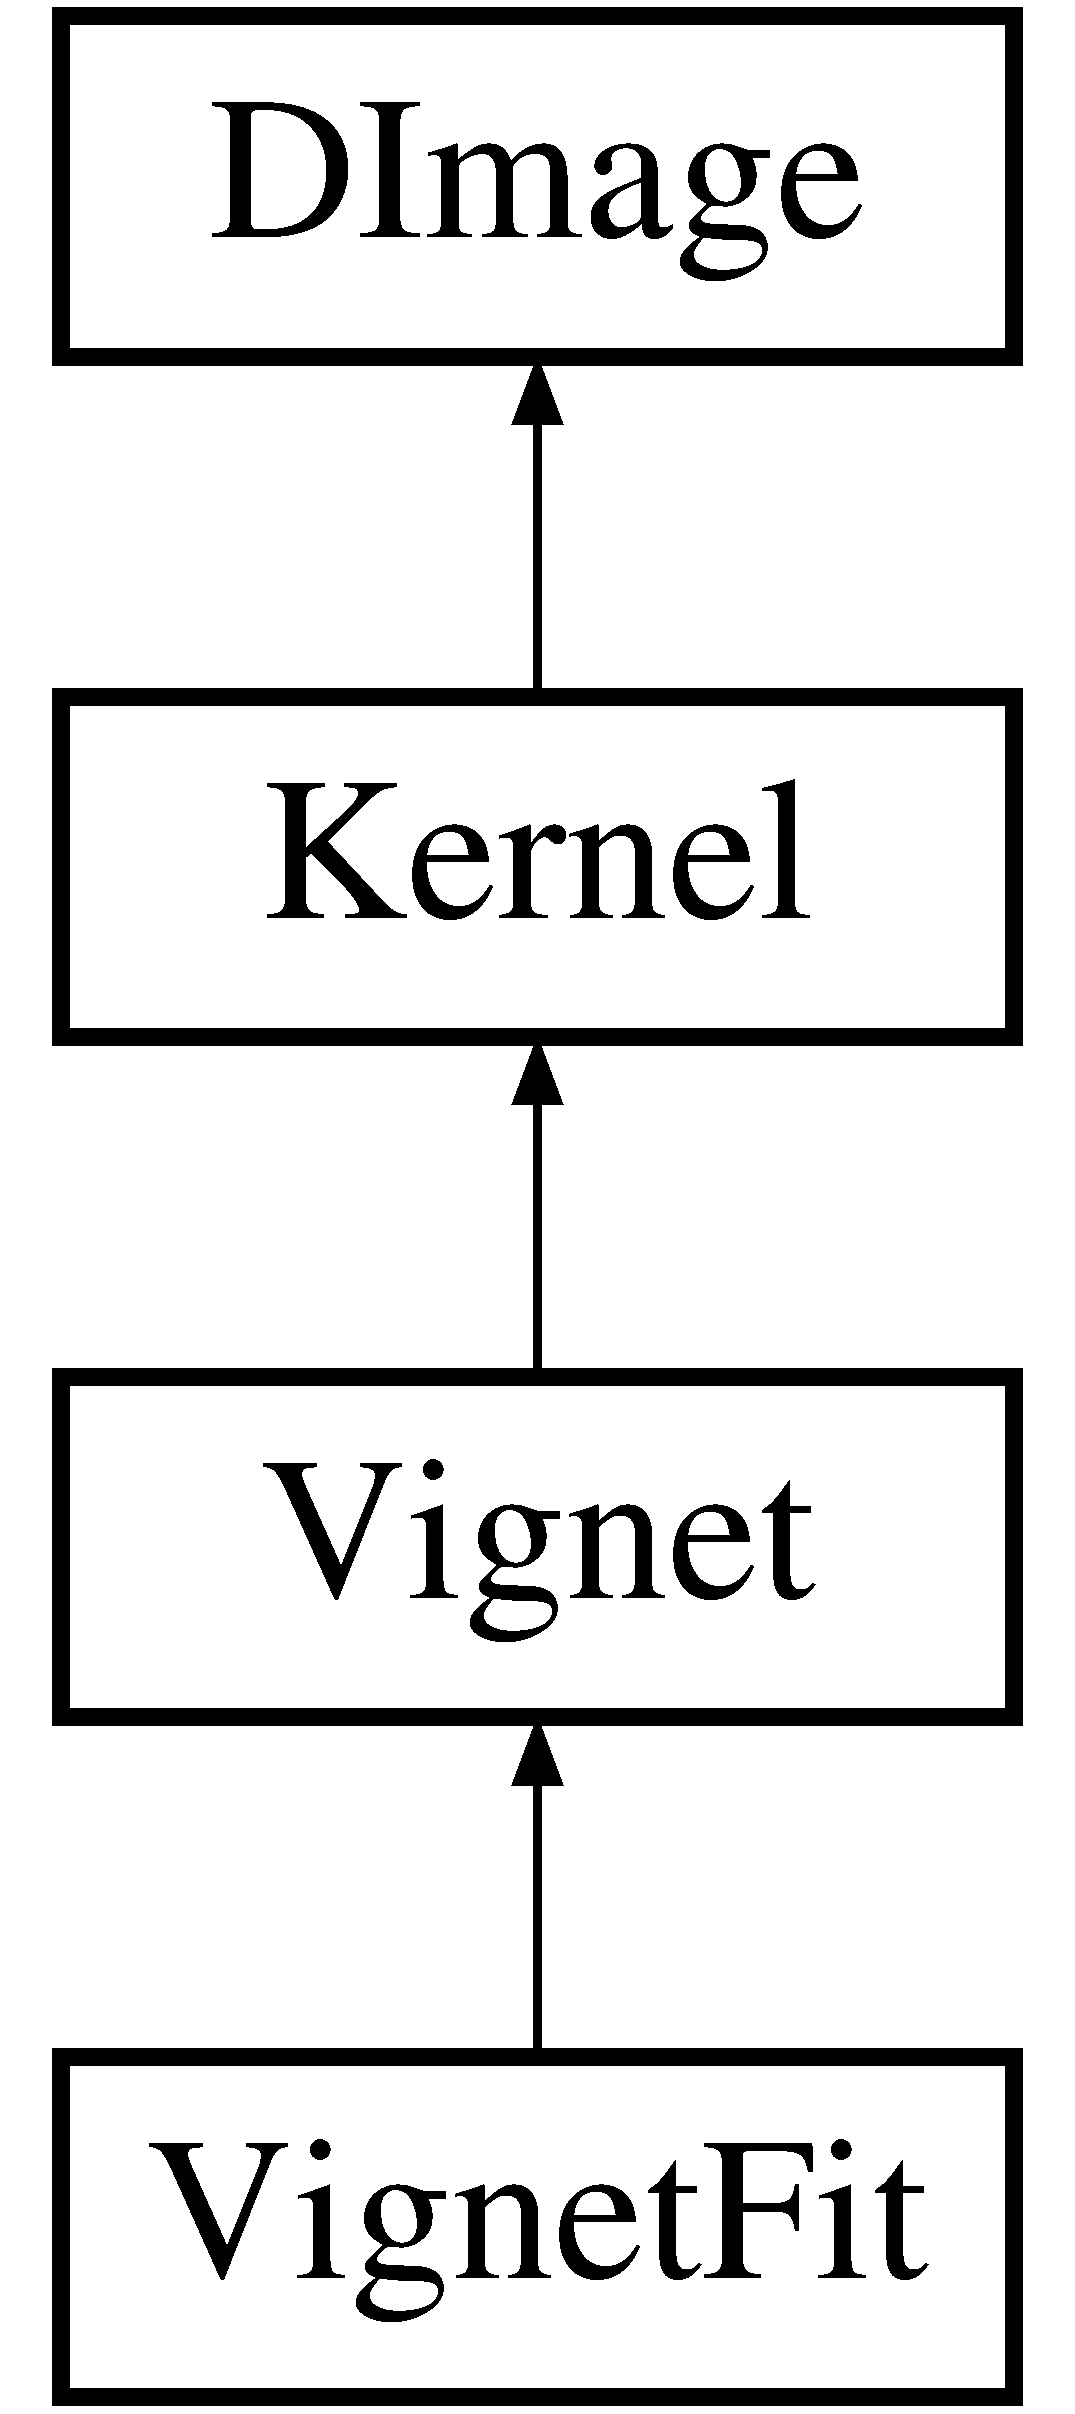
\includegraphics[height=4cm]{class_dimage}
\end{center}
\end{figure}
\subsubsection*{Public Methods}
\begin{CompactItemize}
\item 
\index{DImage@{DImage}!DImage@{DImage}}\index{DImage@{DImage}!DImage@{DImage}}
{\bf DImage} (const int Nx, const int Ny)\label{class_dimage_a0}

\item 
\index{DImage@{DImage}!DImage@{DImage}}\index{DImage@{DImage}!DImage@{DImage}}
{\bf DImage} ()\label{class_dimage_a1}

\item 
\index{Allocate@{Allocate}!DImage@{DImage}}\index{DImage@{DImage}!Allocate@{Allocate}}
void {\bf Allocate} (const int Nx, const int Ny, int Init=1)\label{class_dimage_a2}

\item 
\index{~DImage@{$\sim$DImage}!DImage@{DImage}}\index{DImage@{DImage}!~DImage@{$\sim$DImage}}
{\bf $\sim$DImage} ()\label{class_dimage_a3}

\item 
\index{operator()@{operator()}!DImage@{DImage}}\index{DImage@{DImage}!operator()@{operator()}}
DPixel\& {\bf operator()} (const int i, const int j) const\label{class_dimage_a4}

\begin{CompactList}\small\item\em value on (i,j).\item\end{CompactList}\item 
\index{begin@{begin}!DImage@{DImage}}\index{DImage@{DImage}!begin@{begin}}
DPixel$\ast$ {\bf begin} () const\label{class_dimage_a5}

\begin{CompactList}\small\item\em acces to pointer on first pixel of array.\item\end{CompactList}\item 
\index{Nx@{Nx}!DImage@{DImage}}\index{DImage@{DImage}!Nx@{Nx}}
int {\bf Nx} () const\label{class_dimage_a6}

\item 
\index{Ny@{Ny}!DImage@{DImage}}\index{DImage@{DImage}!Ny@{Ny}}
int {\bf Ny} () const\label{class_dimage_a7}

\item 
\index{Zero@{Zero}!DImage@{DImage}}\index{DImage@{DImage}!Zero@{Zero}}
void {\bf Zero} ()\label{class_dimage_a8}

\begin{CompactList}\small\item\em set all pixels to zero.\item\end{CompactList}\item 
\index{MinValue@{MinValue}!DImage@{DImage}}\index{DImage@{DImage}!MinValue@{Min\-Value}}
DPixel {\bf Min\-Value} () const\label{class_dimage_a9}

\begin{CompactList}\small\item\em returns the minimum pixel value.\item\end{CompactList}\item 
\index{MaxValue@{MaxValue}!DImage@{DImage}}\index{DImage@{DImage}!MaxValue@{Max\-Value}}
DPixel {\bf Max\-Value} () const\label{class_dimage_a10}

\begin{CompactList}\small\item\em returns the maximum pixel value.\item\end{CompactList}\item 
\index{MinMaxValue@{MinMaxValue}!DImage@{DImage}}\index{DImage@{DImage}!MinMaxValue@{Min\-Max\-Value}}
void {\bf Min\-Max\-Value} (DPixel \&Min, DPixel \&Max) const\label{class_dimage_a11}

\begin{CompactList}\small\item\em returns both min and max in a single image traversal.\item\end{CompactList}\item 
\index{DImage@{DImage}!DImage@{DImage}}\index{DImage@{DImage}!DImage@{DImage}}
{\bf DImage} (const DImage \&Other)\label{class_dimage_a12}

\item 
\index{dump@{dump}!DImage@{DImage}}\index{DImage@{DImage}!dump@{dump}}
void {\bf dump} ()\label{class_dimage_a13}

\item 
\index{sum@{sum}!DImage@{DImage}}\index{DImage@{DImage}!sum@{sum}}
DPixel {\bf sum} () const\label{class_dimage_a14}

\begin{CompactList}\small\item\em sum of all pixels.\item\end{CompactList}\item 
\index{Normalize@{Normalize}!DImage@{DImage}}\index{DImage@{DImage}!Normalize@{Normalize}}
void {\bf Normalize} ()\label{class_dimage_a15}

\begin{CompactList}\small\item\em normalize the full DImage.\item\end{CompactList}\item 
\index{operator=@{operator=}!DImage@{DImage}}\index{DImage@{DImage}!operator=@{operator=}}
DImage\& {\bf operator=} (const DImage \&)\label{class_dimage_a16}

\begin{CompactList}\small\item\em handy operators.\item\end{CompactList}\item 
\index{operator=@{operator=}!DImage@{DImage}}\index{DImage@{DImage}!operator=@{operator=}}
DImage\& {\bf operator=} (const {\bf Image} \&)\label{class_dimage_a17}

\item 
\index{operator+=@{operator+=}!DImage@{DImage}}\index{DImage@{DImage}!operator+=@{operator+=}}
DImage\& {\bf operator+=} (const DImage \&Right)\label{class_dimage_a18}

\item 
\index{operator-=@{operator-=}!DImage@{DImage}}\index{DImage@{DImage}!operator-=@{operator-=}}
DImage\& {\bf operator-=} (const DImage \&Right)\label{class_dimage_a19}

\item 
\index{operator *=@{operator $\ast$=}!DImage@{DImage}}\index{DImage@{DImage}!operator *=@{operator $\ast$=}}
DImage\& {\bf operator $\ast$=} (const double \&Right)\label{class_dimage_a20}

\item 
\index{operator *=@{operator $\ast$=}!DImage@{DImage}}\index{DImage@{DImage}!operator *=@{operator $\ast$=}}
DImage\& {\bf operator $\ast$=} (const DImage \&Right)\label{class_dimage_a21}

\item 
\index{operator/=@{operator/=}!DImage@{DImage}}\index{DImage@{DImage}!operator/=@{operator/=}}
DImage\& {\bf operator/=} (const double \&Right)\label{class_dimage_a22}

\item 
\index{operator/=@{operator/=}!DImage@{DImage}}\index{DImage@{DImage}!operator/=@{operator/=}}
DImage\& {\bf operator/=} (const DImage \&Right)\label{class_dimage_a23}

\item 
\index{operator+=@{operator+=}!DImage@{DImage}}\index{DImage@{DImage}!operator+=@{operator+=}}
DImage\& {\bf operator+=} (const double \&Right)\label{class_dimage_a24}

\item 
\index{operator-=@{operator-=}!DImage@{DImage}}\index{DImage@{DImage}!operator-=@{operator-=}}
DImage\& {\bf operator-=} (const double \&Right)\label{class_dimage_a25}

\item 
\index{operator=@{operator=}!DImage@{DImage}}\index{DImage@{DImage}!operator=@{operator=}}
DImage\& {\bf operator=} (const double \&Right)\label{class_dimage_a26}

\item 
\index{readFits@{readFits}!DImage@{DImage}}\index{DImage@{DImage}!readFits@{read\-Fits}}
void {\bf read\-Fits} (const string \&Fits\-Name)\label{class_dimage_a27}

\begin{CompactList}\small\item\em write and read the DImage as a FITS array.\item\end{CompactList}\item 
\index{writeFits@{writeFits}!DImage@{DImage}}\index{DImage@{DImage}!writeFits@{write\-Fits}}
void {\bf write\-Fits} (const string \&Fits\-Name) const\label{class_dimage_a28}

\item 
\index{DImage@{DImage}!DImage@{DImage}}\index{DImage@{DImage}!DImage@{DImage}}
{\bf DImage} (const string \&Fits\-Name)\label{class_dimage_a29}

\begin{CompactList}\small\item\em constructor calls read routine.\item\end{CompactList}\end{CompactItemize}
\subsubsection*{Protected Attributes}
\begin{CompactItemize}
\item 
\index{data00@{data00}!DImage@{DImage}}\index{DImage@{DImage}!data00@{data00}}
DPixel$\ast$ {\bf data00}\label{class_dimage_n0}

\item 
\index{minindex@{minindex}!DImage@{DImage}}\index{DImage@{DImage}!minindex@{minindex}}
int {\bf minindex}\label{class_dimage_n1}

\item 
\index{maxindex@{maxindex}!DImage@{DImage}}\index{DImage@{DImage}!maxindex@{maxindex}}
int {\bf maxindex}\label{class_dimage_n2}

\end{CompactItemize}


\subsubsection{Detailed Description}
a double precision image type.



The documentation for this class was generated from the following file:\begin{CompactItemize}
\item 
{\bf dimage.h}\end{CompactItemize}

\subsection{Fast\-Finder  Class Reference}
\label{class_fastfinder}\index{FastFinder@{Fast\-Finder}}
Fast locator in starlists. 


{\tt \#include $<$fastfinder.h$>$}

\subsubsection*{Public Methods}
\begin{CompactItemize}
\item 
\index{FastFinder@{FastFinder}!FastFinder@{Fast\-Finder}}\index{FastFinder@{FastFinder}!FastFinder@{Fast\-Finder}}
{\bf Fast\-Finder} (const Base\-Star\-List \&List)\label{class_fastfinder_a0}

\begin{CompactList}\small\item\em -.\item\end{CompactList}\item 
\index{~FastFinder@{$\sim$FastFinder}!FastFinder@{Fast\-Finder}}\index{FastFinder@{FastFinder}!~FastFinder@{$\sim$Fast\-Finder}}
{\bf $\sim$Fast\-Finder} ()\label{class_fastfinder_a1}

\item 
\index{FindClosest@{FindClosest}!FastFinder@{Fast\-Finder}}\index{FastFinder@{FastFinder}!FindClosest@{Find\-Closest}}
const {\bf Base\-Star}$\ast$ {\bf Find\-Closest} (const {\bf Point} \&Where, const double Max\-Dist, bool($\ast$Skip\-It)(const {\bf Base\-Star} $\ast$)=NULL) const\label{class_fastfinder_a2}

\begin{CompactList}\small\item\em -.\item\end{CompactList}\item 
\index{dump@{dump}!FastFinder@{Fast\-Finder}}\index{FastFinder@{FastFinder}!dump@{dump}}
void {\bf dump} () const\label{class_fastfinder_a3}

\item 
\index{begin_scan@{begin\_\-scan}!FastFinder@{Fast\-Finder}}\index{FastFinder@{FastFinder}!begin_scan@{begin\_\-scan}}
Iterator {\bf begin\_\-scan} (const {\bf Point} \&Where, const double \&Max\-Dist) const\label{class_fastfinder_a4}

\item 
\index{yslice@{yslice}!FastFinder@{Fast\-Finder}}\index{FastFinder@{FastFinder}!yslice@{yslice}}
void {\bf yslice} (const int i\-Slice, const double YStart, const double YEnd, const {\bf Base\-Star} $\ast$$\ast$\&Start, const {\bf Base\-Star} $\ast$$\ast$\&End) const\label{class_fastfinder_a5}

\item 
\index{locate_y_start@{locate\_\-y\_\-start}!FastFinder@{Fast\-Finder}}\index{FastFinder@{FastFinder}!locate_y_start@{locate\_\-y\_\-start}}
const {\bf Base\-Star}$\ast$$\ast$ {\bf locate\_\-y\_\-start} (const {\bf Base\-Star} $\ast$$\ast$Begin, const {\bf Base\-Star} $\ast$$\ast$End, const double \&YVal) const\label{class_fastfinder_a6}

\item 
\index{locate_y_end@{locate\_\-y\_\-end}!FastFinder@{Fast\-Finder}}\index{FastFinder@{FastFinder}!locate_y_end@{locate\_\-y\_\-end}}
const {\bf Base\-Star}$\ast$$\ast$ {\bf locate\_\-y\_\-end} (const {\bf Base\-Star} $\ast$$\ast$Begin, const {\bf Base\-Star} $\ast$$\ast$End, const double \&YVal) const\label{class_fastfinder_a7}

\end{CompactItemize}
\subsubsection*{Public Attributes}
\begin{CompactItemize}
\item 
\index{stars@{stars}!FastFinder@{Fast\-Finder}}\index{FastFinder@{FastFinder}!stars@{stars}}
const {\bf Base\-Star}$\ast$$\ast$ {\bf stars}\label{class_fastfinder_m0}

\item 
\index{xmin@{xmin}!FastFinder@{Fast\-Finder}}\index{FastFinder@{FastFinder}!xmin@{xmin}}
double {\bf xmin}\label{class_fastfinder_m1}

\item 
\index{xmax@{xmax}!FastFinder@{Fast\-Finder}}\index{FastFinder@{FastFinder}!xmax@{xmax}}
double {\bf xmax}\label{class_fastfinder_m2}

\item 
\index{xstep@{xstep}!FastFinder@{Fast\-Finder}}\index{FastFinder@{FastFinder}!xstep@{xstep}}
double {\bf xstep}\label{class_fastfinder_m3}

\item 
\index{nslice@{nslice}!FastFinder@{Fast\-Finder}}\index{FastFinder@{FastFinder}!nslice@{nslice}}
int {\bf nslice}\label{class_fastfinder_m4}

\item 
\index{index@{index}!FastFinder@{Fast\-Finder}}\index{FastFinder@{FastFinder}!index@{index}}
int$\ast$ {\bf index}\label{class_fastfinder_m5}

\item 
\index{count@{count}!FastFinder@{Fast\-Finder}}\index{FastFinder@{FastFinder}!count@{count}}
int {\bf count}\label{class_fastfinder_m6}

\item 
\index{baselist@{baselist}!FastFinder@{Fast\-Finder}}\index{FastFinder@{FastFinder}!baselist@{baselist}}
const Base\-Star\-List$\ast$ {\bf baselist}\label{class_fastfinder_m7}

\end{CompactItemize}


\subsubsection{Detailed Description}
Fast locator in starlists.

This is an auxillary class for matching objects from starlists. It allows to locate rapidly the closest objects from a given position. The very simple strategy is to sort objects according to 1 coordinate x, and to build an index that allows to select the objects with the x coordinate inside an interval. Then every slice in x is sorted according to y, which enables  a fast scan inside a x slice. List\-Match\-Collect takes about 10ms (PC 450 MHz, optimized \char`\"{}-O4\char`\"{})  for a match between lists of about 2000 objects each, which is fast enough for our needs. The same \char`\"{}locator\char`\"{} is used in List\-Matchup\-Shift, to avoid scanning the whole input lists. Timing on List\-Match\-Collect and List\-Matchup\-Shift indicates a gain in speed by more than one order after implementation of this Fast\-Finder. One should not delete objects in the list passed to the  Fast\-Finder constructor during the whole life of the Fast\-Finder object. 



The documentation for this class was generated from the following file:\begin{CompactItemize}
\item 
{\bf fastfinder.h}\end{CompactItemize}

\subsection{Fits\-Header  Class Reference}
\label{class_fitsheader}\index{FitsHeader@{Fits\-Header}}
Fits files and header keys. 


{\tt \#include $<$fitsimage.h$>$}

Inheritance diagram for Fits\-Header::\begin{figure}[H]
\begin{center}
\leavevmode
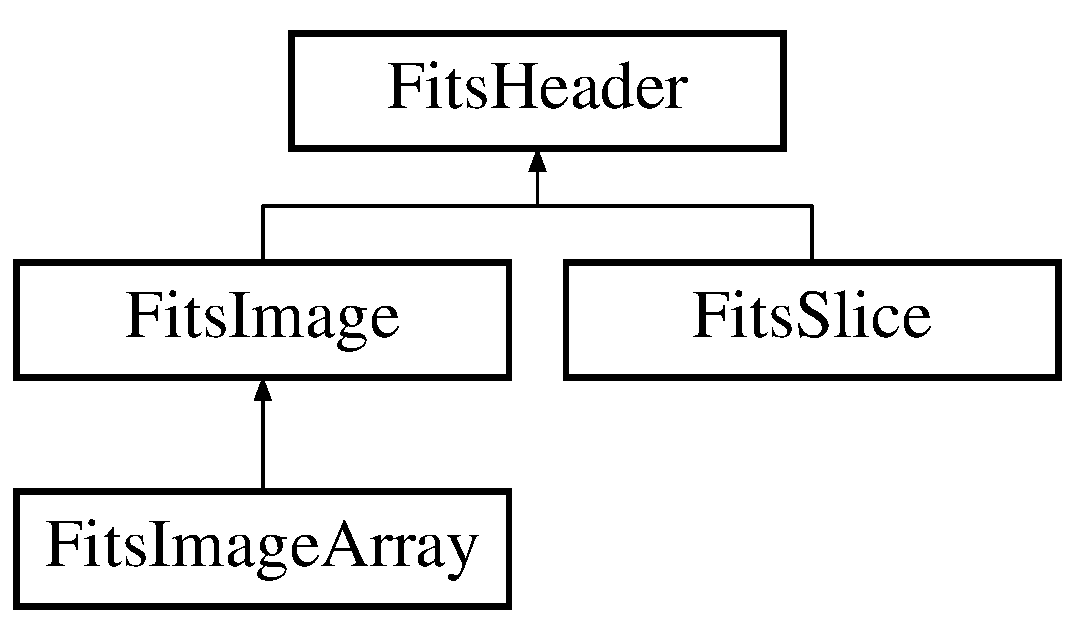
\includegraphics[height=3cm]{class_fitsheader}
\end{center}
\end{figure}
\subsubsection*{Public Methods}
\begin{CompactItemize}
\item 
\index{FitsHeader@{FitsHeader}!FitsHeader@{Fits\-Header}}\index{FitsHeader@{FitsHeader}!FitsHeader@{Fits\-Header}}
{\bf Fits\-Header} ()\label{class_fitsheader_a0}

\item 
\index{FitsHeader@{FitsHeader}!FitsHeader@{Fits\-Header}}\index{FitsHeader@{FitsHeader}!FitsHeader@{Fits\-Header}}
{\bf Fits\-Header} (const string \&File\-Name, const Fits\-File\-Mode Mode=RO, bool Empty\-File=false)\label{class_fitsheader_a1}

\begin{CompactList}\small\item\em opens the file, by default in readonly mode.\item\end{CompactList}\item 
\index{FitsHeader@{FitsHeader}!FitsHeader@{Fits\-Header}}\index{FitsHeader@{FitsHeader}!FitsHeader@{Fits\-Header}}
{\bf Fits\-Header} (const Fits\-Header \&a\_\-header, const string \&New\-File\-Name)\label{class_fitsheader_a2}

\begin{CompactList}\small\item\em opens a new file and copies a old header into it.\item\end{CompactList}\item 
\index{~FitsHeader@{$\sim$FitsHeader}!FitsHeader@{Fits\-Header}}\index{FitsHeader@{FitsHeader}!~FitsHeader@{$\sim$Fits\-Header}}
{\bf $\sim$Fits\-Header} ()\label{class_fitsheader_a3}

\item 
\index{IsValid@{IsValid}!FitsHeader@{Fits\-Header}}\index{FitsHeader@{FitsHeader}!IsValid@{Is\-Valid}}
bool {\bf Is\-Valid} () const\label{class_fitsheader_a4}

\begin{CompactList}\small\item\em returns if the file could be opened.\item\end{CompactList}\item 
\index{FileName@{FileName}!FitsHeader@{Fits\-Header}}\index{FitsHeader@{FitsHeader}!FileName@{File\-Name}}
string {\bf File\-Name} () const\label{class_fitsheader_a5}

\begin{CompactList}\small\item\em access routine to the fits file name.\item\end{CompactList}\item 
\index{FileMode@{FileMode}!FitsHeader@{Fits\-Header}}\index{FitsHeader@{FitsHeader}!FileMode@{File\-Mode}}
Fits\-File\-Mode {\bf File\-Mode} () const\label{class_fitsheader_a6}

\begin{CompactList}\small\item\em return the file mode (RO or RW).\item\end{CompactList}\item 
{\bf Fits\-Key} {\bf Key\-Val} (const string \&Key\-Name, const bool Warn=false) const
\begin{CompactList}\small\item\em read a key. warns on request.\item\end{CompactList}\item 
\index{KeyVal_Secure@{KeyVal\_\-Secure}!FitsHeader@{Fits\-Header}}\index{FitsHeader@{FitsHeader}!KeyVal_Secure@{Key\-Val\_\-Secure}}
{\bf Fits\-Key} {\bf Key\-Val\_\-Secure} (const string \&Key\-Name) const\label{class_fitsheader_a8}

\begin{CompactList}\small\item\em same above but test the presence of the key, and exit if not present.\item\end{CompactList}\item 
int {\bf Mod\-Key} (const string \&Key\-Name, const int Value, const string Comment=\char`\"{}\char`\"{}) const
\begin{CompactList}\small\item\em modifies an existing key value and comment.\item\end{CompactList}\item 
\index{ModKey@{ModKey}!FitsHeader@{Fits\-Header}}\index{FitsHeader@{FitsHeader}!ModKey@{Mod\-Key}}
int {\bf Mod\-Key} (const string \&Key\-Name, const double Value, const string Comment=\char`\"{}\char`\"{}) const\label{class_fitsheader_a10}

\begin{CompactList}\small\item\em -.\item\end{CompactList}\item 
\index{ModKey@{ModKey}!FitsHeader@{Fits\-Header}}\index{FitsHeader@{FitsHeader}!ModKey@{Mod\-Key}}
int {\bf Mod\-Key} (const string \&Key\-Name, const char $\ast$Value, const string Comment=\char`\"{}\char`\"{}) const\label{class_fitsheader_a11}

\begin{CompactList}\small\item\em -.\item\end{CompactList}\item 
\index{ModKey@{ModKey}!FitsHeader@{Fits\-Header}}\index{FitsHeader@{FitsHeader}!ModKey@{Mod\-Key}}
int {\bf Mod\-Key} (const string \&Key\-Name, const bool Value, const string Comment=\char`\"{}\char`\"{}) const\label{class_fitsheader_a12}

\begin{CompactList}\small\item\em -.\item\end{CompactList}\item 
int {\bf Add\-Key} (const string \&Key\-Name, const char $\ast$Key\-Val, const string Comment=\char`\"{}\char`\"{})
\begin{CompactList}\small\item\em adds (at the end of the header) a new key.\item\end{CompactList}\item 
\index{AddKey@{AddKey}!FitsHeader@{Fits\-Header}}\index{FitsHeader@{FitsHeader}!AddKey@{Add\-Key}}
int {\bf Add\-Key} (const string \&Key\-Name, const double Key\-Val, const string Comment=\char`\"{}\char`\"{})\label{class_fitsheader_a14}

\item 
\index{AddKey@{AddKey}!FitsHeader@{Fits\-Header}}\index{FitsHeader@{FitsHeader}!AddKey@{Add\-Key}}
int {\bf Add\-Key} (const string \&Key\-Name, const int Key\-Val, const string Comment=\char`\"{}\char`\"{})\label{class_fitsheader_a15}

\item 
\index{AddKey@{AddKey}!FitsHeader@{Fits\-Header}}\index{FitsHeader@{FitsHeader}!AddKey@{Add\-Key}}
int {\bf Add\-Key} (const string \&Key\-Name, const bool Key\-Val, const string Comment=\char`\"{}\char`\"{})\label{class_fitsheader_a16}

\item 
\index{AddOrModKey@{AddOrModKey}!FitsHeader@{Fits\-Header}}\index{FitsHeader@{FitsHeader}!AddOrModKey@{Add\-Or\-Mod\-Key}}
int {\bf Add\-Or\-Mod\-Key} (const string \&Key\-Name, const char $\ast$Value, const string Comment=\char`\"{}\char`\"{})\label{class_fitsheader_a17}

\begin{CompactList}\small\item\em modifies an existing key or adds it if it does not exist yet.\item\end{CompactList}\item 
\index{AddOrModKey@{AddOrModKey}!FitsHeader@{Fits\-Header}}\index{FitsHeader@{FitsHeader}!AddOrModKey@{Add\-Or\-Mod\-Key}}
int {\bf Add\-Or\-Mod\-Key} (const string \&Key\-Name, const string \&Value, const string Comment=\char`\"{}\char`\"{})\label{class_fitsheader_a18}

\begin{CompactList}\small\item\em modifies an existing key or adds it if it does not exist yet.\item\end{CompactList}\item 
\index{AddOrModKey@{AddOrModKey}!FitsHeader@{Fits\-Header}}\index{FitsHeader@{FitsHeader}!AddOrModKey@{Add\-Or\-Mod\-Key}}
int {\bf Add\-Or\-Mod\-Key} (const string \&Key\-Name, const double Value, const string Comment=\char`\"{}\char`\"{})\label{class_fitsheader_a19}

\begin{CompactList}\small\item\em modifies an existing key or adds it if it does not exist yet.\item\end{CompactList}\item 
\index{AddOrModKey@{AddOrModKey}!FitsHeader@{Fits\-Header}}\index{FitsHeader@{FitsHeader}!AddOrModKey@{Add\-Or\-Mod\-Key}}
int {\bf Add\-Or\-Mod\-Key} (const string \&Key\-Name, const int Value, const string Comment=\char`\"{}\char`\"{})\label{class_fitsheader_a20}

\begin{CompactList}\small\item\em modifies an existing key or adds it if it does not exist yet.\item\end{CompactList}\item 
\index{AddOrModKey@{AddOrModKey}!FitsHeader@{Fits\-Header}}\index{FitsHeader@{FitsHeader}!AddOrModKey@{Add\-Or\-Mod\-Key}}
int {\bf Add\-Or\-Mod\-Key} (const string \&Key\-Name, const bool Value, const string Comment=\char`\"{}\char`\"{})\label{class_fitsheader_a21}

\begin{CompactList}\small\item\em modifies an existing key or adds it if it does not exist yet.\item\end{CompactList}\item 
int {\bf Key\-Match} (const string \&Key\-Pattern, Fits\-Key\-Array \&Array) const
\begin{CompactList}\small\item\em To read keys following a pattern.\item\end{CompactList}\item 
\index{ModKeyName@{ModKeyName}!FitsHeader@{Fits\-Header}}\index{FitsHeader@{FitsHeader}!ModKeyName@{Mod\-Key\-Name}}
int {\bf Mod\-Key\-Name} (const string \&Old\-Key\-Name, const string \&New\-Key\-Name) const\label{class_fitsheader_a23}

\begin{CompactList}\small\item\em changes the Key itself.\item\end{CompactList}\item 
\index{ModKeyComment@{ModKeyComment}!FitsHeader@{Fits\-Header}}\index{FitsHeader@{FitsHeader}!ModKeyComment@{Mod\-Key\-Comment}}
int {\bf Mod\-Key\-Comment} (const string \&Key\-Name, const string \&New\-Comment) const\label{class_fitsheader_a24}

\begin{CompactList}\small\item\em changes the comment.\item\end{CompactList}\item 
\index{HasKey@{HasKey}!FitsHeader@{Fits\-Header}}\index{FitsHeader@{FitsHeader}!HasKey@{Has\-Key}}
bool {\bf Has\-Key} (const string \&Key\-Name, const bool Warn=false) const\label{class_fitsheader_a25}

\begin{CompactList}\small\item\em enables to check the presence of a key. warns on request.\item\end{CompactList}\item 
\index{HasActualKey@{HasActualKey}!FitsHeader@{Fits\-Header}}\index{FitsHeader@{FitsHeader}!HasActualKey@{Has\-Actual\-Key}}
bool {\bf Has\-Actual\-Key} (const string \&Key\-Name, const bool Warn=false) const\label{class_fitsheader_a26}

\begin{CompactList}\small\item\em has a genuine fits key.\item\end{CompactList}\item 
\index{RmKey@{RmKey}!FitsHeader@{Fits\-Header}}\index{FitsHeader@{FitsHeader}!RmKey@{Rm\-Key}}
int {\bf Rm\-Key} (const string \&Key\-Name) const\label{class_fitsheader_a27}

\begin{CompactList}\small\item\em deletes a key.\item\end{CompactList}\item 
\index{NKeys@{NKeys}!FitsHeader@{Fits\-Header}}\index{FitsHeader@{FitsHeader}!NKeys@{NKeys}}
int {\bf NKeys} () const\label{class_fitsheader_a28}

\begin{CompactList}\small\item\em return the number of keys (without counting the END key).\item\end{CompactList}\item 
\index{CopyKey@{CopyKey}!FitsHeader@{Fits\-Header}}\index{FitsHeader@{FitsHeader}!CopyKey@{Copy\-Key}}
bool {\bf Copy\-Key} (const char $\ast$Key\-Name, Fits\-Header \&To) const\label{class_fitsheader_a29}

\begin{CompactList}\small\item\em copy verbatim a key (name, value, comment).\item\end{CompactList}\item 
int {\bf Add\-Comment\-Line} (const string \&AVery\-Useful\-Comment)
\begin{CompactList}\small\item\em add a COMMENT keyword.\item\end{CompactList}\item 
int {\bf Add\-History\-Line} (const string \&History\-Stuff)
\begin{CompactList}\small\item\em add a HISTORY keyword.\item\end{CompactList}\item 
\index{Flush@{Flush}!FitsHeader@{Fits\-Header}}\index{FitsHeader@{FitsHeader}!Flush@{Flush}}
int {\bf Flush} ()\label{class_fitsheader_a32}

\begin{CompactList}\small\item\em flush file buffers.\item\end{CompactList}\item 
\index{AddOrModCard@{AddOrModCard}!FitsHeader@{Fits\-Header}}\index{FitsHeader@{FitsHeader}!AddOrModCard@{Add\-Or\-Mod\-Card}}
int {\bf Add\-Or\-Mod\-Card} (const string \&Key\-Name, const string \&Card)\label{class_fitsheader_a33}

\begin{CompactList}\small\item\em add a whole card, name+value+comment (or modifies an existing one).\item\end{CompactList}\item 
\index{ImageSizes@{ImageSizes}!FitsHeader@{Fits\-Header}}\index{FitsHeader@{FitsHeader}!ImageSizes@{Image\-Sizes}}
void {\bf Image\-Sizes} (int \&Xsize, int \&YSize) const\label{class_fitsheader_a34}

\item 
\index{SameImageSizes@{SameImageSizes}!FitsHeader@{Fits\-Header}}\index{FitsHeader@{FitsHeader}!SameImageSizes@{Same\-Image\-Sizes}}
bool {\bf Same\-Image\-Sizes} (const Fits\-Header \&Other) const\label{class_fitsheader_a35}

\item 
\index{ImageCenter@{ImageCenter}!FitsHeader@{Fits\-Header}}\index{FitsHeader@{FitsHeader}!ImageCenter@{Image\-Center}}
{\bf Point} {\bf Image\-Center} () const\label{class_fitsheader_a36}

\begin{CompactList}\small\item\em The geometric center of the image.\item\end{CompactList}\item 
\index{SameChipFilterInst@{SameChipFilterInst}!FitsHeader@{Fits\-Header}}\index{FitsHeader@{FitsHeader}!SameChipFilterInst@{Same\-Chip\-Filter\-Inst}}
bool {\bf Same\-Chip\-Filter\-Inst} (const Fits\-Header \&Other, const bool Warn=true) const\label{class_fitsheader_a37}

\begin{CompactList}\small\item\em checks that both images refer to the same chip, filter and instrument.\item\end{CompactList}\item 
\index{SameChipFilter@{SameChipFilter}!FitsHeader@{Fits\-Header}}\index{FitsHeader@{FitsHeader}!SameChipFilter@{Same\-Chip\-Filter}}
bool {\bf Same\-Chip\-Filter} (const Fits\-Header \&Other, const bool Warn=true) const\label{class_fitsheader_a38}

\begin{CompactList}\small\item\em checks that both images refer to the same chip and filter.\item\end{CompactList}\item 
\index{SameChipFilter@{SameChipFilter}!FitsHeader@{Fits\-Header}}\index{FitsHeader@{FitsHeader}!SameChipFilter@{Same\-Chip\-Filter}}
bool {\bf Same\-Chip\-Filter} (const string \&Other\-Fits\-Name, const bool Warn=true) const\label{class_fitsheader_a39}

\item 
\index{SameFilter@{SameFilter}!FitsHeader@{Fits\-Header}}\index{FitsHeader@{FitsHeader}!SameFilter@{Same\-Filter}}
bool {\bf Same\-Filter} (const Fits\-Header \&Other, const bool Warn=true) const\label{class_fitsheader_a40}

\begin{CompactList}\small\item\em checks that both images refer to the same filter.\item\end{CompactList}\item 
\index{SameFilter@{SameFilter}!FitsHeader@{Fits\-Header}}\index{FitsHeader@{FitsHeader}!SameFilter@{Same\-Filter}}
bool {\bf Same\-Filter} (const string \&Other\-Fits\-Name, const bool Warn=true) const\label{class_fitsheader_a41}

\item 
\index{SameChip@{SameChip}!FitsHeader@{Fits\-Header}}\index{FitsHeader@{FitsHeader}!SameChip@{Same\-Chip}}
bool {\bf Same\-Chip} (const Fits\-Header \&Other, const bool Warn=true) const\label{class_fitsheader_a42}

\begin{CompactList}\small\item\em checks that both images refer to the same chip.\item\end{CompactList}\item 
\index{SameChip@{SameChip}!FitsHeader@{Fits\-Header}}\index{FitsHeader@{FitsHeader}!SameChip@{Same\-Chip}}
bool {\bf Same\-Chip} (const string \&Other\-Fits\-Name, const bool Warn=true) const\label{class_fitsheader_a43}

\begin{CompactList}\small\item\em same as above, using file name.\item\end{CompactList}\item 
\index{TelInst@{TelInst}!FitsHeader@{Fits\-Header}}\index{FitsHeader@{FitsHeader}!TelInst@{Tel\-Inst}}
Virtual\-Instrument$\ast$ {\bf Tel\-Inst} () const\label{class_fitsheader_a44}

\item 
void {\bf Enable\-Write} (const bool Yes\-Or\-No)
\begin{CompactList}\small\item\em for a {\bf Fits\-Image} {\rm (p.\,\pageref{class_fitsimage})} opened RW, enables to forbid writing (default behaviour) when destructor is called.\item\end{CompactList}\item 
\index{FitsHeader@{FitsHeader}!FitsHeader@{Fits\-Header}}\index{FitsHeader@{FitsHeader}!FitsHeader@{Fits\-Header}}
{\bf Fits\-Header} (const Fits\-Header \&)\label{class_fitsheader_a46}

\item 
\index{Append_LowPriority@{Append\_\-LowPriority}!FitsHeader@{Fits\-Header}}\index{FitsHeader@{FitsHeader}!Append_LowPriority@{Append\_\-Low\-Priority}}
void {\bf Append\_\-Low\-Priority} (const Fits\-Header \&To\-Append)\label{class_fitsheader_a47}

\item 
\index{MoveHDU@{MoveHDU}!FitsHeader@{Fits\-Header}}\index{FitsHeader@{FitsHeader}!MoveHDU@{Move\-HDU}}
int {\bf Move\-HDU} (int How\-Many=1)\label{class_fitsheader_a48}

\item 
\index{CopyCHDUTo@{CopyCHDUTo}!FitsHeader@{Fits\-Header}}\index{FitsHeader@{FitsHeader}!CopyCHDUTo@{Copy\-CHDUTo}}
int {\bf Copy\-CHDUTo} (Fits\-Header \&Out\-Header)\label{class_fitsheader_a49}

\item 
\index{CopyDataTo@{CopyDataTo}!FitsHeader@{Fits\-Header}}\index{FitsHeader@{FitsHeader}!CopyDataTo@{Copy\-Data\-To}}
int {\bf Copy\-Data\-To} (Fits\-Header \&Out\-Header)\label{class_fitsheader_a50}

\item 
\index{NHDU@{NHDU}!FitsHeader@{Fits\-Header}}\index{FitsHeader@{FitsHeader}!NHDU@{NHDU}}
int {\bf NHDU} () const\label{class_fitsheader_a51}

\end{CompactItemize}
\subsubsection*{Friends}
\begin{CompactItemize}
\item 
class {\bf Fits\-Image\-Array}
\item 
class {\bf Fits\-Key}
\item 
class {\bf Fits\-Image}
\item 
class {\bf Fits\-Slice}
\item 
\index{operator<<@{operator$<$$<$}!FitsHeader@{Fits\-Header}}\index{FitsHeader@{FitsHeader}!operator<<@{operator$<$$<$}}
ostream\& {\bf operator$<$$<$} (ostream \&stream, const Fits\-Header \&Header)\label{class_fitsheader_l4}

\begin{CompactList}\small\item\em enables : \footnotesize\begin{verbatim} cout << FitsHeader("my_image.fits"); \end{verbatim}\normalsize 
.\item\end{CompactList}\end{CompactItemize}


\subsubsection{Detailed Description}
Fits files and header keys.

The Fits\-Header class does not deal with the data part of fits files. The actual engine is cfitsio. 



\subsubsection{Member Function Documentation}
\index{FitsHeader@{Fits\-Header}!AddCommentLine@{AddCommentLine}}
\index{AddCommentLine@{AddCommentLine}!FitsHeader@{Fits\-Header}}
\paragraph{\setlength{\rightskip}{0pt plus 5cm}int Fits\-Header::Add\-Comment\-Line (const string \& {\em AVery\-Useful\-Comment})}\hfill\label{class_fitsheader_a30}


add a COMMENT keyword.

It will be split over multiple  COMMENT lines if longer than 70 characters. \index{FitsHeader@{Fits\-Header}!AddHistoryLine@{AddHistoryLine}}
\index{AddHistoryLine@{AddHistoryLine}!FitsHeader@{Fits\-Header}}
\paragraph{\setlength{\rightskip}{0pt plus 5cm}int Fits\-Header::Add\-History\-Line (const string \& {\em History\-Stuff})}\hfill\label{class_fitsheader_a31}


add a HISTORY keyword.

It will be split over multiple  HISTORY lines if longer than 70 characters. \index{FitsHeader@{Fits\-Header}!AddKey@{AddKey}}
\index{AddKey@{AddKey}!FitsHeader@{Fits\-Header}}
\paragraph{\setlength{\rightskip}{0pt plus 5cm}int Fits\-Header::Add\-Key (const string \& {\em Key\-Name}, const char $\ast$ {\em Key\-Val}, const string {\em Comment} = \char`\"{}\char`\"{})}\hfill\label{class_fitsheader_a13}


adds (at the end of the header) a new key.

Checks before that this key does not exist yet. No comment if Comment is NULL or absent. Value can be int, double, char$\ast$, or bool. \index{FitsHeader@{Fits\-Header}!EnableWrite@{EnableWrite}}
\index{EnableWrite@{EnableWrite}!FitsHeader@{Fits\-Header}}
\paragraph{\setlength{\rightskip}{0pt plus 5cm}void Fits\-Header::Enable\-Write (const bool {\em Yes\-Or\-No})}\hfill\label{class_fitsheader_a45}


for a {\bf Fits\-Image} {\rm (p.\,\pageref{class_fitsimage})} opened RW, enables to forbid writing (default behaviour) when destructor is called.

example of use : the flatfielding opens (RW) the flatfielded {\bf Fits\-Image} {\rm (p.\,\pageref{class_fitsimage})}, and  only allow writing on successful flatfielding completion. \index{FitsHeader@{Fits\-Header}!KeyMatch@{KeyMatch}}
\index{KeyMatch@{KeyMatch}!FitsHeader@{Fits\-Header}}
\paragraph{\setlength{\rightskip}{0pt plus 5cm}int Fits\-Header::Key\-Match (const string \& {\em Key\-Pattern}, Fits\-Key\-Array \& {\em Array}) const}\hfill\label{class_fitsheader_a22}


To read keys following a pattern.

$\ast$ matches anything, ? a single character, \# successive decimal digits. Array[i]. size() returns the number of matched keys. Array[i].Key\-Name and \{double,string,int\}(Array[i]) enable to accees  key names and values \index{FitsHeader@{Fits\-Header}!KeyVal@{KeyVal}}
\index{KeyVal@{KeyVal}!FitsHeader@{Fits\-Header}}
\paragraph{\setlength{\rightskip}{0pt plus 5cm}{\bf Fits\-Key} Fits\-Header::Key\-Val (const string \& {\em Key\-Name}, const bool {\em Warn} = false) const}\hfill\label{class_fitsheader_a7}


read a key. warns on request.

use (e.g.) \footnotesize\begin{verbatim} double ra = a_header.KeyVal("RA"); \end{verbatim}\normalsize 
 adequate converters are applied for int, double, float, string and bool variables. \index{FitsHeader@{Fits\-Header}!ModKey@{ModKey}}
\index{ModKey@{ModKey}!FitsHeader@{Fits\-Header}}
\paragraph{\setlength{\rightskip}{0pt plus 5cm}int Fits\-Header::Mod\-Key (const string \& {\em Key\-Name}, const int {\em Value}, const string {\em Comment} = \char`\"{}\char`\"{}) const}\hfill\label{class_fitsheader_a9}


modifies an existing key value and comment.

If comment is NULL the comment is unchanged. 

The documentation for this class was generated from the following file:\begin{CompactItemize}
\item 
{\bf fitsimage.h}\end{CompactItemize}

\subsection{Fits\-Image  Class Reference}
\label{class_fitsimage}\index{FitsImage@{Fits\-Image}}
This class enables basic manipulation of images stored in fits files. 


{\tt \#include $<$fitsimage.h$>$}

Inheritance diagram for Fits\-Image::\begin{figure}[H]
\begin{center}
\leavevmode
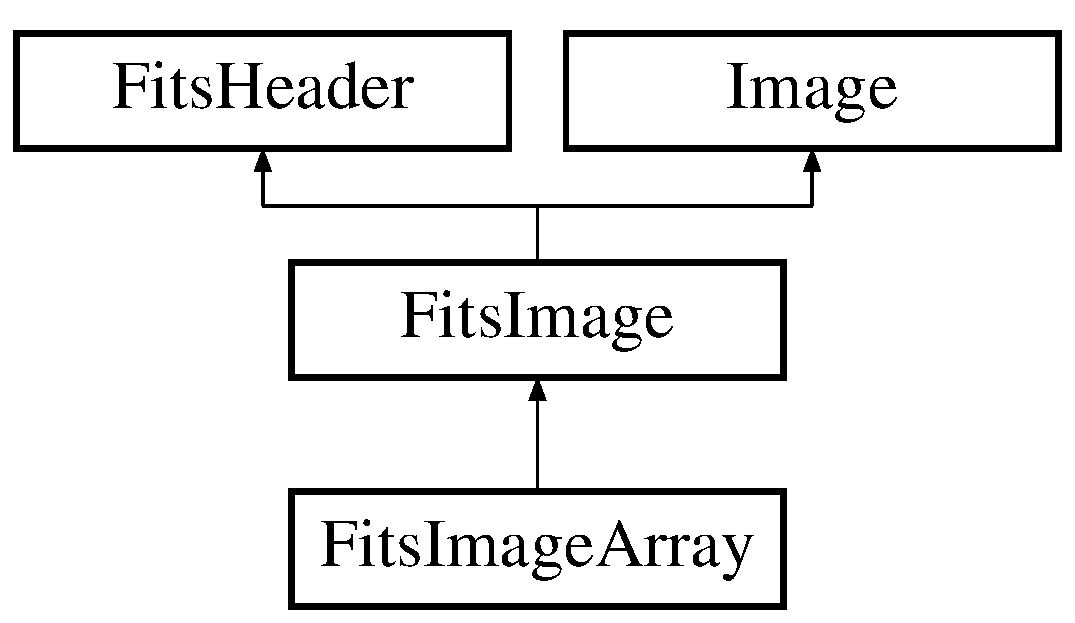
\includegraphics[height=3cm]{class_fitsimage}
\end{center}
\end{figure}
\subsubsection*{Public Methods}
\begin{CompactItemize}
\item 
\index{FitsImage@{FitsImage}!FitsImage@{Fits\-Image}}\index{FitsImage@{FitsImage}!FitsImage@{Fits\-Image}}
{\bf Fits\-Image} (const string \&File\-Name, const Fits\-File\-Mode Mode=RO)\label{class_fitsimage_a0}

\begin{CompactList}\small\item\em opens in (Read\-Only mode by default, use RW to modifiy or create) and loads the pixel data.\item\end{CompactList}\item 
\index{FitsImage@{FitsImage}!FitsImage@{Fits\-Image}}\index{FitsImage@{FitsImage}!FitsImage@{Fits\-Image}}
{\bf Fits\-Image} (const {\bf Fits\-Header} \&Header)\label{class_fitsimage_a1}

\begin{CompactList}\small\item\em constructor to be used starting from an existing {\bf Fits\-Header} {\rm (p.\,\pageref{class_fitsheader})}.\item\end{CompactList}\item 
{\bf Fits\-Image} (const string \&New\-File\-Name, const {\bf Fits\-Header} \&a\_\-fits\_\-header, const {\bf Image} \&an\_\-image)
\begin{CompactList}\small\item\em constructor for a new Fits\-Image.\item\end{CompactList}\item 
\index{FitsImage@{FitsImage}!FitsImage@{Fits\-Image}}\index{FitsImage@{FitsImage}!FitsImage@{Fits\-Image}}
{\bf Fits\-Image} (const string \&New\-File\-Name, const {\bf Fits\-Header} \&AHeader)\label{class_fitsimage_a3}

\begin{CompactList}\small\item\em constructor of a new Fits\-Image using an existing header, a new name, and a zeroed {\bf Image} {\rm (p.\,\pageref{class_image})}. RW mode.\item\end{CompactList}\item 
\index{FitsImage@{FitsImage}!FitsImage@{Fits\-Image}}\index{FitsImage@{FitsImage}!FitsImage@{Fits\-Image}}
{\bf Fits\-Image} (const string \&File\-Name, const {\bf Image} \&an\_\-image)\label{class_fitsimage_a4}

\begin{CompactList}\small\item\em constructor for a new Fits\-Image with a minimal header from an existing image.\item\end{CompactList}\item 
\index{FitsImage@{FitsImage}!FitsImage@{Fits\-Image}}\index{FitsImage@{FitsImage}!FitsImage@{Fits\-Image}}
{\bf Fits\-Image} (const string \&File\-Name, const int Nx, const int Ny)\label{class_fitsimage_a5}

\begin{CompactList}\small\item\em constructor for a new Fits\-Image with a minimal header from scratch.\item\end{CompactList}\item 
\index{Trim@{Trim}!FitsImage@{Fits\-Image}}\index{FitsImage@{FitsImage}!Trim@{Trim}}
void {\bf Trim} (const {\bf Frame} \&Region)\label{class_fitsimage_a6}

\begin{CompactList}\small\item\em Extract and replaces the trimed {\bf Image} {\rm (p.\,\pageref{class_image})} into a Fits\-Image.\item\end{CompactList}\item 
\index{PreserveZeros@{PreserveZeros}!FitsImage@{Fits\-Image}}\index{FitsImage@{FitsImage}!PreserveZeros@{Preserve\-Zeros}}
void {\bf Preserve\-Zeros} ()\label{class_fitsimage_a7}

\begin{CompactList}\small\item\em This routine is to be called if one wants to preserve the value of 0 on I/O. Assumes contents $>$=0, as it is Used for weight maps.\item\end{CompactList}\item 
\index{~FitsImage@{$\sim$FitsImage}!FitsImage@{Fits\-Image}}\index{FitsImage@{FitsImage}!~FitsImage@{$\sim$Fits\-Image}}
{\bf $\sim$Fits\-Image} ()\label{class_fitsimage_a8}

\item 
\index{SetWriteAsFloat@{SetWriteAsFloat}!FitsImage@{Fits\-Image}}\index{FitsImage@{FitsImage}!SetWriteAsFloat@{Set\-Write\-As\-Float}}
bool {\bf Set\-Write\-As\-Float} ()\label{class_fitsimage_a9}

\item 
\index{Write@{Write}!FitsImage@{Fits\-Image}}\index{FitsImage@{FitsImage}!Write@{Write}}
int {\bf Write} (bool force\_\-bscale=false)\label{class_fitsimage_a10}

\item 
\index{Write@{Write}!FitsImage@{Fits\-Image}}\index{FitsImage@{FitsImage}!Write@{Write}}
int {\bf Write} (const double \&Bscale, const double \&Bzero)\label{class_fitsimage_a11}

\end{CompactItemize}


\subsubsection{Detailed Description}
This class enables basic manipulation of images stored in fits files.

For The image itself, see the {\bf Image} {\rm (p.\,\pageref{class_image})} class. The files opened in mode RW are actually written to disk by the destructor. {\bf Fits\-Header::Enable\-Write}() {\rm (p.\,\pageref{class_fitsheader_a45})} allows to alter this default behavior. 



\subsubsection{Constructor \& Destructor Documentation}
\index{FitsImage@{Fits\-Image}!FitsImage@{FitsImage}}
\index{FitsImage@{FitsImage}!FitsImage@{Fits\-Image}}
\paragraph{\setlength{\rightskip}{0pt plus 5cm}Fits\-Image::Fits\-Image (const string \& {\em New\-File\-Name}, const {\bf Fits\-Header} \& {\em a\_\-fits\_\-header}, const {\bf Image} \& {\em an\_\-image})}\hfill\label{class_fitsimage_a2}


constructor for a new Fits\-Image.

To be used to assemble a Fits\-Image from a header and an image obtained separately. The associated mode is RW. The actual size of the saved image is the one of the image, not the one in the header. 

The documentation for this class was generated from the following file:\begin{CompactItemize}
\item 
{\bf fitsimage.h}\end{CompactItemize}

\subsection{Fits\-Image\-Array  Class Reference}
\label{class_fitsimagearray}\index{FitsImageArray@{Fits\-Image\-Array}}
Array of {\bf Image} {\rm (p.\,\pageref{class_image})} in a FITS file. 


{\tt \#include $<$fitsimagearray.h$>$}

Inheritance diagram for Fits\-Image\-Array::\begin{figure}[H]
\begin{center}
\leavevmode
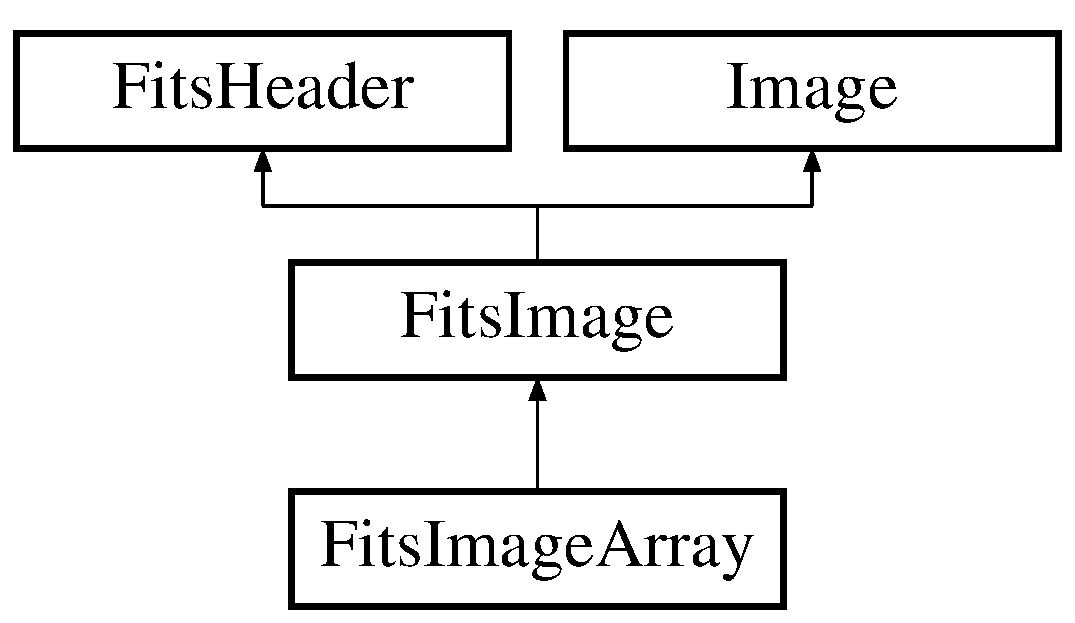
\includegraphics[height=3cm]{class_fitsimagearray}
\end{center}
\end{figure}
\subsubsection*{Public Types}
\begin{CompactItemize}
\item 
enum {\bf Status} \{ {\bf OK} =  0, 
{\bf OUTOFBOUNDS} =  1, 
{\bf FAILURE} =  2, 
{\bf ERRORWRITE} =  3, 
{\bf EMPTY} =  4
 \}
\begin{CompactList}\small\item\em Status flag for all functions.\item\end{CompactList}\item 
enum {\bf Criterion} \{ {\bf CHIP} =  1, 
{\bf FILTER} =  2, 
{\bf SIZE} =  4, 
{\bf EXTENDED} =  8
 \}
\begin{CompactList}\small\item\em Criterion fo image selection.\item\end{CompactList}\end{CompactItemize}
\subsubsection*{Public Methods}
\begin{CompactItemize}
\item 
{\bf Fits\-Image\-Array} (const string \&File\-Name, const Fits\-File\-Mode Mode=RO)
\begin{CompactList}\small\item\em Constructor for an existing fits image.\item\end{CompactList}\item 
{\bf Fits\-Image\-Array} (const string \&File\-Name, const {\bf Fits\-Header} \&header, bool Image\-In\-First\-HDU=true)
\begin{CompactList}\small\item\em Constructor for a new Fits\-Image\-Array with a minimal header from an existing {\bf Fits\-Header} {\rm (p.\,\pageref{class_fitsheader})}.\item\end{CompactList}\item 
{\bf Fits\-Image\-Array} (const string \&File\-Name, const {\bf Image} \&image, bool Image\-In\-First\-HDU=true)
\begin{CompactList}\small\item\em Constructor for a new Fits\-Image\-Array with a minimal header from an existing {\bf Image} {\rm (p.\,\pageref{class_image})}.\item\end{CompactList}\item 
\index{~FitsImageArray@{$\sim$FitsImageArray}!FitsImageArray@{Fits\-Image\-Array}}\index{FitsImageArray@{FitsImageArray}!~FitsImageArray@{$\sim$Fits\-Image\-Array}}
{\bf $\sim$Fits\-Image\-Array} ()\label{class_fitsimagearray_a3}

\begin{CompactList}\small\item\em Standard destructor.\item\end{CompactList}\item 
\index{Write@{Write}!FitsImageArray@{Fits\-Image\-Array}}\index{FitsImageArray@{FitsImageArray}!Write@{Write}}
{\bf Status} {\bf Write} (bool force\_\-bscale=false)\label{class_fitsimagearray_a4}

\begin{CompactList}\small\item\em Write all images to the FITS file.\item\end{CompactList}\item 
\index{SplitAndWrite@{SplitAndWrite}!FitsImageArray@{Fits\-Image\-Array}}\index{FitsImageArray@{FitsImageArray}!SplitAndWrite@{Split\-And\-Write}}
{\bf Status} {\bf Split\-And\-Write} (const string \&directory=\char`\"{}\char`\"{},int HDUMax=0)\label{class_fitsimagearray_a5}

\begin{CompactList}\small\item\em Write all images to separated FITS files (same as split\_\-fits).\item\end{CompactList}\item 
{\bf Status} {\bf Append} (const string \&filename)
\begin{CompactList}\small\item\em Add a {\bf Fits\-Image} {\rm (p.\,\pageref{class_fitsimage})} after the latest HDU.\item\end{CompactList}\item 
{\bf Status} {\bf Append} (const {\bf Image} \&image)
\begin{CompactList}\small\item\em Add an {\bf Image} {\rm (p.\,\pageref{class_image})} after the latest HDU.\item\end{CompactList}\item 
\index{At@{At}!FitsImageArray@{Fits\-Image\-Array}}\index{FitsImageArray@{FitsImageArray}!At@{At}}
{\bf Status} {\bf At} (int HDU)\label{class_fitsimagearray_a8}

\begin{CompactList}\small\item\em {\bf Point} {\rm (p.\,\pageref{class_point})} to the image at index HDU ( 1 $<$= HDU $<$= Get\-NImages()).\item\end{CompactList}\item 
\index{Next@{Next}!FitsImageArray@{Fits\-Image\-Array}}\index{FitsImageArray@{FitsImageArray}!Next@{Next}}
{\bf Status} {\bf Next} ()\label{class_fitsimagearray_a9}

\begin{CompactList}\small\item\em {\bf Point} {\rm (p.\,\pageref{class_point})} to the next image.\item\end{CompactList}\item 
void {\bf Set\-Criterion} (int value)
\begin{CompactList}\small\item\em Set the criterion for merging of {\bf Fits\-Image} {\rm (p.\,\pageref{class_fitsimage})}.\item\end{CompactList}\item 
\index{IsValid@{IsValid}!FitsImageArray@{Fits\-Image\-Array}}\index{FitsImageArray@{FitsImageArray}!IsValid@{Is\-Valid}}
bool {\bf Is\-Valid} ()\label{class_fitsimagearray_a11}

\begin{CompactList}\small\item\em Check whether this Fits\-Image\-Array is valid.\item\end{CompactList}\item 
\index{GetVersion@{GetVersion}!FitsImageArray@{Fits\-Image\-Array}}\index{FitsImageArray@{FitsImageArray}!GetVersion@{Get\-Version}}
string {\bf Get\-Version} ()\label{class_fitsimagearray_a12}

\begin{CompactList}\small\item\em Returns the version of this piece of code.\item\end{CompactList}\item 
bool {\bf Check\-Header} ({\bf Fits\-Header} \&header)
\begin{CompactList}\small\item\em Check whether header is consistent with f\-Main\-Header.\item\end{CompactList}\end{CompactItemize}


\subsubsection{Detailed Description}
Array of {\bf Image} {\rm (p.\,\pageref{class_image})} in a FITS file.

Inherites from {\bf Fits\-Image} {\rm (p.\,\pageref{class_fitsimage})} 



\subsubsection{Constructor \& Destructor Documentation}
\index{FitsImageArray@{Fits\-Image\-Array}!FitsImageArray@{FitsImageArray}}
\index{FitsImageArray@{FitsImageArray}!FitsImageArray@{Fits\-Image\-Array}}
\paragraph{\setlength{\rightskip}{0pt plus 5cm}Fits\-Image\-Array::Fits\-Image\-Array (const string \& {\em File\-Name}, const Fits\-File\-Mode {\em Mode} = RO)}\hfill\label{class_fitsimagearray_a0}


Constructor for an existing fits image.

\begin{CompactItemize}
\item 
 Opens in (Read\-Only (RO) mode by default, use RW to modify or create) \item 
 In RW mode, use this creator for an image already containing several images, i.e. with EXTEND=true (if EXTEND=false, {\bf Is\-Valid}() {\rm (p.\,\pageref{class_fitsimagearray_a11})}=false) \end{CompactItemize}
\index{FitsImageArray@{Fits\-Image\-Array}!FitsImageArray@{FitsImageArray}}
\index{FitsImageArray@{FitsImageArray}!FitsImageArray@{Fits\-Image\-Array}}
\paragraph{\setlength{\rightskip}{0pt plus 5cm}Fits\-Image\-Array::Fits\-Image\-Array (const string \& {\em File\-Name}, const {\bf Fits\-Header} \& {\em header}, bool {\em Image\-In\-First\-HDU} = true)}\hfill\label{class_fitsimagearray_a1}


Constructor for a new Fits\-Image\-Array with a minimal header from an existing {\bf Fits\-Header} {\rm (p.\,\pageref{class_fitsheader})}.

This header is used as a reference for image size, filter, chip. A criterion for accepting images can be set with the function Set\-Criterion  using the values of the enum {\bf Fits\-Image\-Array::Criterion} {\rm (p.\,\pageref{class_fitsimagearray_s10})}.  For instance Set\-Criterion(Fits\-Image\-Array::FILTER$|$Fits\-Image\-Array::CHIP) $<$=$>$ ask for the same filter and chip.\begin{Desc}
\item[{\bf Parameters: }]\par
\begin{description}
\item[
{\em Image\-In\-First\-HDU, if}]true (default) the first image that is added is saved in the first HDU, otherwise it is saved in the second one. \end{description}
\end{Desc}
\index{FitsImageArray@{Fits\-Image\-Array}!FitsImageArray@{FitsImageArray}}
\index{FitsImageArray@{FitsImageArray}!FitsImageArray@{Fits\-Image\-Array}}
\paragraph{\setlength{\rightskip}{0pt plus 5cm}Fits\-Image\-Array::Fits\-Image\-Array (const string \& {\em File\-Name}, const {\bf Image} \& {\em image}, bool {\em Image\-In\-First\-HDU} = true)}\hfill\label{class_fitsimagearray_a2}


Constructor for a new Fits\-Image\-Array with a minimal header from an existing {\bf Image} {\rm (p.\,\pageref{class_image})}.

This {\bf Image} {\rm (p.\,\pageref{class_image})} is used as a reference for image size (see previous constructor). The user can define other keys for accepting other images.\begin{Desc}
\item[{\bf Parameters: }]\par
\begin{description}
\item[
{\em Image\-In\-First\-HDU, if}]true (default) the first image that is added is saved in the first HDU, otherwise it is saved in the second one. \end{description}
\end{Desc}


\subsubsection{Member Function Documentation}
\index{FitsImageArray@{Fits\-Image\-Array}!Append@{Append}}
\index{Append@{Append}!FitsImageArray@{Fits\-Image\-Array}}
\paragraph{\setlength{\rightskip}{0pt plus 5cm}{\bf Status} Fits\-Image\-Array::Append (const {\bf Image} \& {\em image})}\hfill\label{class_fitsimagearray_a7}


Add an {\bf Image} {\rm (p.\,\pageref{class_image})} after the latest HDU.

\begin{Desc}
\item[{\bf Parameters: }]\par
\begin{description}
\item[
{\em Image}]that is appended. \begin{CompactItemize}
\item 
 A default {\bf Fits\-Header} {\rm (p.\,\pageref{class_fitsheader})} is written, namely with NAXIS$\ast$,  BSCALE, BZERO, BITPIX=16, and WRITEDAT \item 
 The user may add information to the header after the call to this function \end{CompactItemize}
\end{description}
\end{Desc}
\index{FitsImageArray@{Fits\-Image\-Array}!Append@{Append}}
\index{Append@{Append}!FitsImageArray@{Fits\-Image\-Array}}
\paragraph{\setlength{\rightskip}{0pt plus 5cm}{\bf Status} Fits\-Image\-Array::Append (const string \& {\em filename})}\hfill\label{class_fitsimagearray_a6}


Add a {\bf Fits\-Image} {\rm (p.\,\pageref{class_fitsimage})} after the latest HDU.

\begin{Desc}
\item[{\bf Parameters: }]\par
\begin{description}
\item[
{\em filename, name}]of the fits file to append Uses cfitsio fits\_\-copy\_\-hdu, i.e. toads is not used a lot except for checking the compatibility of {\bf Fits\-Header} {\rm (p.\,\pageref{class_fitsheader})} \end{description}
\end{Desc}
\index{FitsImageArray@{Fits\-Image\-Array}!CheckHeader@{CheckHeader}}
\index{CheckHeader@{CheckHeader}!FitsImageArray@{Fits\-Image\-Array}}
\paragraph{\setlength{\rightskip}{0pt plus 5cm}bool Fits\-Image\-Array::Check\-Header ({\bf Fits\-Header} \& {\em header})}\hfill\label{class_fitsimagearray_a13}


Check whether header is consistent with f\-Main\-Header.

\begin{CompactItemize}
\item 
 Used by {\bf Fits\-Image\-Array::Append} {\rm (p.\,\pageref{class_fitsimagearray_a6})} \item 
 Uses f\-Selected\-Criterion (see Set\-Criterion) \end{CompactItemize}
\index{FitsImageArray@{Fits\-Image\-Array}!SetCriterion@{SetCriterion}}
\index{SetCriterion@{SetCriterion}!FitsImageArray@{Fits\-Image\-Array}}
\paragraph{\setlength{\rightskip}{0pt plus 5cm}void Fits\-Image\-Array::Set\-Criterion (int {\em value})\hspace{0.3cm}{\tt  [inline]}}\hfill\label{class_fitsimagearray_a10}


Set the criterion for merging of {\bf Fits\-Image} {\rm (p.\,\pageref{class_fitsimage})}.

\begin{Desc}
\item[{\bf Parameters: }]\par
\begin{description}
\item[
{\em value}]: example Fits\-Image\-Array::CHIP$|$Fits\-Image\-Array::FILTER \end{description}
\end{Desc}


The documentation for this class was generated from the following file:\begin{CompactItemize}
\item 
{\bf fitsimagearray.h}\end{CompactItemize}

\subsection{Fits\-Key  Class Reference}
\label{class_fitskey}\index{FitsKey@{Fits\-Key}}
Auxilary class for accessing fits header keys. 


{\tt \#include $<$fitsimage.h$>$}

\subsubsection*{Public Methods}
\begin{CompactItemize}
\item 
\index{FitsKey@{FitsKey}!FitsKey@{Fits\-Key}}\index{FitsKey@{FitsKey}!FitsKey@{Fits\-Key}}
{\bf Fits\-Key} (const string \&Key\-Name, const double \&val)\label{class_fitskey_a0}

\item 
\index{FitsKey@{FitsKey}!FitsKey@{Fits\-Key}}\index{FitsKey@{FitsKey}!FitsKey@{Fits\-Key}}
{\bf Fits\-Key} (const string \&Key\-Name, const int val)\label{class_fitskey_a1}

\item 
\index{FitsKey@{FitsKey}!FitsKey@{Fits\-Key}}\index{FitsKey@{FitsKey}!FitsKey@{Fits\-Key}}
{\bf Fits\-Key} (const string \&Key\-Name, const string \&val)\label{class_fitskey_a2}

\item 
\index{operator int@{operator int}!FitsKey@{Fits\-Key}}\index{FitsKey@{FitsKey}!operator int@{operator int}}
{\bf operator int} ()\label{class_fitskey_a3}

\item 
\index{operator float@{operator float}!FitsKey@{Fits\-Key}}\index{FitsKey@{FitsKey}!operator float@{operator float}}
{\bf operator float} ()\label{class_fitskey_a4}

\item 
\index{operator double@{operator double}!FitsKey@{Fits\-Key}}\index{FitsKey@{FitsKey}!operator double@{operator double}}
{\bf operator double} ()\label{class_fitskey_a5}

\item 
\index{operator string@{operator string}!FitsKey@{Fits\-Key}}\index{FitsKey@{FitsKey}!operator string@{operator string}}
{\bf operator string} ()\label{class_fitskey_a6}

\item 
\index{operator bool@{operator bool}!FitsKey@{Fits\-Key}}\index{FitsKey@{FitsKey}!operator bool@{operator bool}}
{\bf operator bool} ()\label{class_fitskey_a7}

\item 
\index{KeyName@{KeyName}!FitsKey@{Fits\-Key}}\index{FitsKey@{FitsKey}!KeyName@{Key\-Name}}
string {\bf Key\-Name} () const\label{class_fitskey_a8}

\end{CompactItemize}
\subsubsection*{Friends}
\begin{CompactItemize}
\item 
class {\bf Fits\-Header}
\item 
class {\bf operator$<$$<$}
\end{CompactItemize}


\subsubsection{Detailed Description}
Auxilary class for accessing fits header keys.



The documentation for this class was generated from the following file:\begin{CompactItemize}
\item 
{\bf fitsimage.h}\end{CompactItemize}

\subsection{Fits\-Parallel\-Slices  Class Reference}
\label{class_fitsparallelslices}\index{FitsParallelSlices@{Fits\-Parallel\-Slices}}
Several fits images of the same size to be processed in parallel. 


{\tt \#include $<$fitsslice.h$>$}

Inheritance diagram for Fits\-Parallel\-Slices::\begin{figure}[H]
\begin{center}
\leavevmode
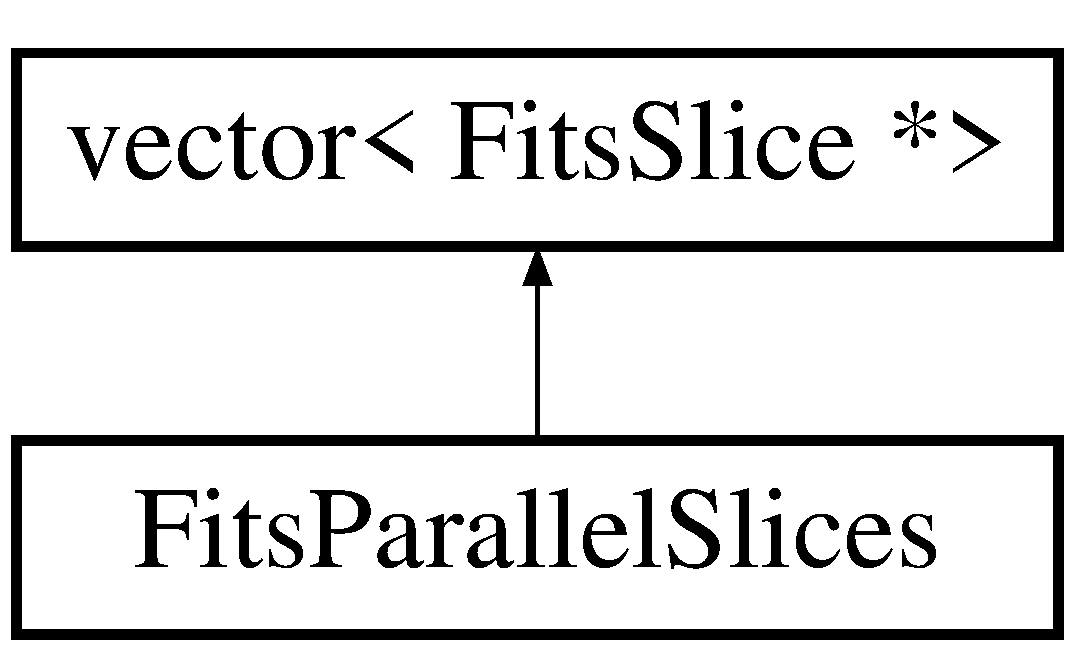
\includegraphics[height=2cm]{class_fitsparallelslices}
\end{center}
\end{figure}
\subsubsection*{Public Methods}
\begin{CompactItemize}
\item 
\index{FitsParallelSlices@{FitsParallelSlices}!FitsParallelSlices@{Fits\-Parallel\-Slices}}\index{FitsParallelSlices@{FitsParallelSlices}!FitsParallelSlices@{Fits\-Parallel\-Slices}}
{\bf Fits\-Parallel\-Slices} (const int Slice\-Size, const int Overlap=0)\label{class_fitsparallelslices_a0}

\begin{CompactList}\small\item\em constructor.\item\end{CompactList}\item 
\index{~FitsParallelSlices@{$\sim$FitsParallelSlices}!FitsParallelSlices@{Fits\-Parallel\-Slices}}\index{FitsParallelSlices@{FitsParallelSlices}!~FitsParallelSlices@{$\sim$Fits\-Parallel\-Slices}}
{\bf $\sim$Fits\-Parallel\-Slices} ()\label{class_fitsparallelslices_a1}

\item 
\index{AddFile@{AddFile}!FitsParallelSlices@{Fits\-Parallel\-Slices}}\index{FitsParallelSlices@{FitsParallelSlices}!AddFile@{Add\-File}}
bool {\bf Add\-File} (const string \&File\-Name)\label{class_fitsparallelslices_a2}

\begin{CompactList}\small\item\em Adds a file in the list. Loads the first slice.\item\end{CompactList}\item 
\index{LoadNextSlice@{LoadNextSlice}!FitsParallelSlices@{Fits\-Parallel\-Slices}}\index{FitsParallelSlices@{FitsParallelSlices}!LoadNextSlice@{Load\-Next\-Slice}}
int {\bf Load\-Next\-Slice} ()\label{class_fitsparallelslices_a3}

\begin{CompactList}\small\item\em load next slice for all involved files. Returns 0 if already on last slice.\item\end{CompactList}\item 
\index{SliceSize@{SliceSize}!FitsParallelSlices@{Fits\-Parallel\-Slices}}\index{FitsParallelSlices@{FitsParallelSlices}!SliceSize@{Slice\-Size}}
int {\bf Slice\-Size} () const\label{class_fitsparallelslices_a4}

\begin{CompactList}\small\item\em size of the current slice size. Different from the constructor value for last slice.\item\end{CompactList}\item 
\index{ImageJ@{ImageJ}!FitsParallelSlices@{Fits\-Parallel\-Slices}}\index{FitsParallelSlices@{FitsParallelSlices}!ImageJ@{Image\-J}}
int {\bf Image\-J} (const int Slice\-J) const\label{class_fitsparallelslices_a5}

\begin{CompactList}\small\item\em return the index in the whole image of the row Slice\-J in the current slice.\item\end{CompactList}\item 
\index{LastSlice@{LastSlice}!FitsParallelSlices@{Fits\-Parallel\-Slices}}\index{FitsParallelSlices@{FitsParallelSlices}!LastSlice@{Last\-Slice}}
bool {\bf Last\-Slice} () const\label{class_fitsparallelslices_a6}

\begin{CompactList}\small\item\em are we in the last slice.\item\end{CompactList}\item 
\index{NFiles@{NFiles}!FitsParallelSlices@{Fits\-Parallel\-Slices}}\index{FitsParallelSlices@{FitsParallelSlices}!NFiles@{NFiles}}
int {\bf NFiles} () const\label{class_fitsparallelslices_a7}

\end{CompactItemize}


\subsubsection{Detailed Description}
Several fits images of the same size to be processed in parallel.

This class is to be used as a handler for {\bf Fits\-Slice} {\rm (p.\,\pageref{class_fitsslice})}'s from files having the same sizes, that one wants to process in parallel (typically to average or sum images). Slices are cut along the second index of the whole image  and have the same size in x as the image.  See {\bf Usage of Fits\-Parallel\-Slices} {\rm (p.\,\pageref{example_slices})} for an example. 



The documentation for this class was generated from the following file:\begin{CompactItemize}
\item 
{\bf fitsslice.h}\end{CompactItemize}

\subsection{Fits\-Set  Class Reference}
\label{class_fitsset}\index{FitsSet@{Fits\-Set}}
container for fits files that have same sizes, filter, and come from the same chip within a mosaic. 


{\tt \#include $<$fitsset.h$>$}

\subsubsection*{Public Methods}
\begin{CompactItemize}
\item 
{\bf Fits\-Set} (const string \&File\-Name, const bool Check\-Filter=true)
\begin{CompactList}\small\item\em constructor from a file that contains file names (one per line).\item\end{CompactList}\item 
\index{operator[]@{operator[]}!FitsSet@{Fits\-Set}}\index{FitsSet@{FitsSet}!operator[]@{operator[$\,$]}}
string {\bf operator[$\,$]} (const unsigned int i) const\label{class_fitsset_a1}

\item 
\index{size@{size}!FitsSet@{Fits\-Set}}\index{FitsSet@{FitsSet}!size@{size}}
int {\bf size} () const\label{class_fitsset_a2}

\begin{CompactList}\small\item\em Number of file in the set.\item\end{CompactList}\item 
\index{AllNames@{AllNames}!FitsSet@{Fits\-Set}}\index{FitsSet@{FitsSet}!AllNames@{All\-Names}}
string {\bf All\-Names} () const\label{class_fitsset_a3}

\begin{CompactList}\small\item\em returns a string containing all file names.\item\end{CompactList}\item 
\index{Nx@{Nx}!FitsSet@{Fits\-Set}}\index{FitsSet@{FitsSet}!Nx@{Nx}}
int {\bf Nx} () const\label{class_fitsset_a4}

\begin{CompactList}\small\item\em x size of images (excluding overscan if any).\item\end{CompactList}\item 
\index{Ny@{Ny}!FitsSet@{Fits\-Set}}\index{FitsSet@{FitsSet}!Ny@{Ny}}
int {\bf Ny} () const\label{class_fitsset_a5}

\begin{CompactList}\small\item\em y size of images.\item\end{CompactList}\item 
\index{NxTot@{NxTot}!FitsSet@{Fits\-Set}}\index{FitsSet@{FitsSet}!NxTot@{Nx\-Tot}}
int {\bf Nx\-Tot} () const\label{class_fitsset_a6}

\begin{CompactList}\small\item\em total x size of images (including overscan).\item\end{CompactList}\item 
\index{NyTot@{NyTot}!FitsSet@{Fits\-Set}}\index{FitsSet@{FitsSet}!NyTot@{Ny\-Tot}}
int {\bf Ny\-Tot} () const\label{class_fitsset_a7}

\begin{CompactList}\small\item\em same for y.\item\end{CompactList}\end{CompactItemize}


\subsubsection{Detailed Description}
container for fits files that have same sizes, filter, and come from the same chip within a mosaic.



\subsubsection{Constructor \& Destructor Documentation}
\index{FitsSet@{Fits\-Set}!FitsSet@{FitsSet}}
\index{FitsSet@{FitsSet}!FitsSet@{Fits\-Set}}
\paragraph{\setlength{\rightskip}{0pt plus 5cm}Fits\-Set::Fits\-Set (const string \& {\em File\-Name}, const bool {\em Check\-Filter} = true)}\hfill\label{class_fitsset_a0}


constructor from a file that contains file names (one per line).

Those can be actual filenames or {\bf Db\-Image} {\rm (p.\,\pageref{class_dbimage})} names. 

The documentation for this class was generated from the following file:\begin{CompactItemize}
\item 
{\bf fitsset.h}\end{CompactItemize}

\subsection{Fits\-Slice  Class Reference}
\label{class_fitsslice}\index{FitsSlice@{Fits\-Slice}}
Memory saving traversal of a fits image. 


{\tt \#include $<$fitsslice.h$>$}

Inheritance diagram for Fits\-Slice::\begin{figure}[H]
\begin{center}
\leavevmode
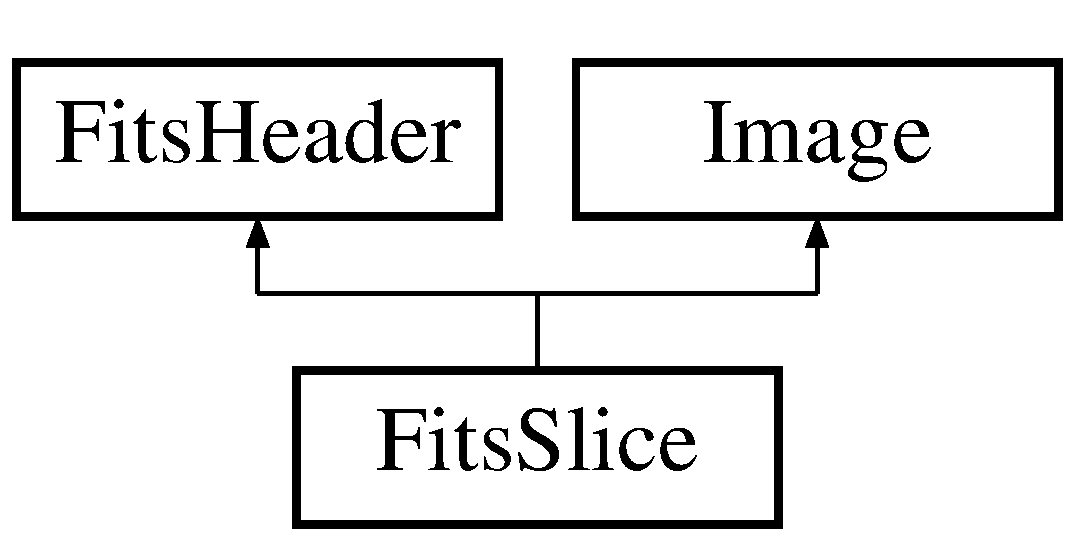
\includegraphics[height=2cm]{class_fitsslice}
\end{center}
\end{figure}
\subsubsection*{Public Methods}
\begin{CompactItemize}
\item 
\index{FitsSlice@{FitsSlice}!FitsSlice@{Fits\-Slice}}\index{FitsSlice@{FitsSlice}!FitsSlice@{Fits\-Slice}}
{\bf Fits\-Slice} (const string File\-Name, const int Slice\-YSize, const int Overlap)\label{class_fitsslice_a0}

\begin{CompactList}\small\item\em constructor. Overlap is the number of rows in common to successive slices (usually 0).\item\end{CompactList}\item 
\index{LoadNextSlice@{LoadNextSlice}!FitsSlice@{Fits\-Slice}}\index{FitsSlice@{FitsSlice}!LoadNextSlice@{Load\-Next\-Slice}}
int {\bf Load\-Next\-Slice} ()\label{class_fitsslice_a1}

\begin{CompactList}\small\item\em load next slice into memory.\item\end{CompactList}\item 
\index{SliceSize@{SliceSize}!FitsSlice@{Fits\-Slice}}\index{FitsSlice@{FitsSlice}!SliceSize@{Slice\-Size}}
int {\bf Slice\-Size} () const\label{class_fitsslice_a2}

\begin{CompactList}\small\item\em the current slice size (differs from the constructor value at last slice).\item\end{CompactList}\item 
\index{ImageJ@{ImageJ}!FitsSlice@{Fits\-Slice}}\index{FitsSlice@{FitsSlice}!ImageJ@{Image\-J}}
int {\bf Image\-J} (const int j) const\label{class_fitsslice_a3}

\begin{CompactList}\small\item\em the coordinate in the full image of row j in present slice.\item\end{CompactList}\item 
\index{LastSlice@{LastSlice}!FitsSlice@{Fits\-Slice}}\index{FitsSlice@{FitsSlice}!LastSlice@{Last\-Slice}}
bool {\bf Last\-Slice} () const\label{class_fitsslice_a4}

\begin{CompactList}\small\item\em are we in the last slice?\item\end{CompactList}\end{CompactItemize}


\subsubsection{Detailed Description}
Memory saving traversal of a fits image.

This class is intended to access an image in a fits file, but only a slice of the image will reside in memory at a time. To be used when many images have to be accessed at the same time, in parallel (see {\bf Fits\-Parallel\-Slices} {\rm (p.\,\pageref{class_fitsparallelslices})}), or maybe to traverse a very big image. 



The documentation for this class was generated from the following file:\begin{CompactItemize}
\item 
{\bf fitsslice.h}\end{CompactItemize}

\subsection{Frame  Class Reference}
\label{class_frame}\index{Frame@{Frame}}
rectangle with sides parallel to axes. 


{\tt \#include $<$frame.h$>$}

\subsubsection*{Public Methods}
\begin{CompactItemize}
\item 
\index{Frame@{Frame}!Frame@{Frame}}\index{Frame@{Frame}!Frame@{Frame}}
{\bf Frame} ()\label{class_frame_a0}

\item 
\index{Frame@{Frame}!Frame@{Frame}}\index{Frame@{Frame}!Frame@{Frame}}
{\bf Frame} (const {\bf Image} \&image)\label{class_frame_a1}

\begin{CompactList}\small\item\em actual image frame.\item\end{CompactList}\item 
\index{Frame@{Frame}!Frame@{Frame}}\index{Frame@{Frame}!Frame@{Frame}}
{\bf Frame} (const double \&{\bf x\-Min}, const double \&{\bf y\-Min}, const double \&{\bf x\-Max}, const double \&{\bf y\-Max})\label{class_frame_a2}

\begin{CompactList}\small\item\em this one is dangerous: you may swap the 2 middle arguments. Prefer next one.\item\end{CompactList}\item 
\index{Frame@{Frame}!Frame@{Frame}}\index{Frame@{Frame}!Frame@{Frame}}
{\bf Frame} (const {\bf Point} \&Lower\-Left, const {\bf Point} \&Upper\-Right)\label{class_frame_a3}

\begin{CompactList}\small\item\em typical use: Frame(Point(xmin,ymin),Point(xmax,ymax)).\item\end{CompactList}\item 
\index{Frame@{Frame}!Frame@{Frame}}\index{Frame@{Frame}!Frame@{Frame}}
{\bf Frame} (const {\bf Fits\-Header} \&header, Which\-Frame which=Clipped\-Size\-Frame)\label{class_frame_a4}

\begin{CompactList}\small\item\em 2 kinds of bounds in headers, the chip size and some that may be added by hand. See {\bf Write\-In\-Header}() {\rm (p.\,\pageref{class_frame_a22})}.\item\end{CompactList}\item 
\index{Nx@{Nx}!Frame@{Frame}}\index{Frame@{Frame}!Nx@{Nx}}
double {\bf Nx} () const\label{class_frame_a5}

\begin{CompactList}\small\item\em number of pixels in x direction.\item\end{CompactList}\item 
\index{Ny@{Ny}!Frame@{Frame}}\index{Frame@{Frame}!Ny@{Ny}}
double {\bf Ny} () const\label{class_frame_a6}

\begin{CompactList}\small\item\em number of pixels in y direction.\item\end{CompactList}\item 
\index{Center@{Center}!Frame@{Frame}}\index{Frame@{Frame}!Center@{Center}}
{\bf Point} {\bf Center} () const\label{class_frame_a7}

\begin{CompactList}\small\item\em middle of the frame.\item\end{CompactList}\item 
\index{ApplyTransfo@{ApplyTransfo}!Frame@{Frame}}\index{Frame@{Frame}!ApplyTransfo@{Apply\-Transfo}}
Frame {\bf Apply\-Transfo} (const {\bf Gtransfo} \&T) const\label{class_frame_a8}

\begin{CompactList}\small\item\em assumes that Transfo is a shift or involves a 'simple rotation'.\item\end{CompactList}\item 
\index{operator *@{operator $\ast$}!Frame@{Frame}}\index{Frame@{Frame}!operator *@{operator $\ast$}}
Frame {\bf operator $\ast$} (const Frame \&Right) const\label{class_frame_a9}

\begin{CompactList}\small\item\em intersection of Frame's.\item\end{CompactList}\item 
\index{operator *=@{operator $\ast$=}!Frame@{Frame}}\index{Frame@{Frame}!operator *=@{operator $\ast$=}}
Frame\& {\bf operator $\ast$=} (const Frame \&Right)\label{class_frame_a10}

\begin{CompactList}\small\item\em intersection of Frame's.\item\end{CompactList}\item 
\index{operator+@{operator+}!Frame@{Frame}}\index{Frame@{Frame}!operator+@{operator+}}
Frame {\bf operator+} (const Frame \&Right) const\label{class_frame_a11}

\begin{CompactList}\small\item\em union of Frames.\item\end{CompactList}\item 
\index{operator+=@{operator+=}!Frame@{Frame}}\index{Frame@{Frame}!operator+=@{operator+=}}
Frame\& {\bf operator+=} (const Frame \&Right)\label{class_frame_a12}

\begin{CompactList}\small\item\em union of Frames.\item\end{CompactList}\item 
\index{CutMargin@{CutMargin}!Frame@{Frame}}\index{Frame@{Frame}!CutMargin@{Cut\-Margin}}
void {\bf Cut\-Margin} (const double Margin\-Size)\label{class_frame_a13}

\begin{CompactList}\small\item\em shrinks the frame (if Margin\-Size$>$0), enlarges it (if Margin\-Size$<$0).\item\end{CompactList}\item 
\index{CutMargin@{CutMargin}!Frame@{Frame}}\index{Frame@{Frame}!CutMargin@{Cut\-Margin}}
void {\bf Cut\-Margin} (const double Margin\-X, const double Margin\-Y)\label{class_frame_a14}

\begin{CompactList}\small\item\em shrinks the frame (if Margin\-Size$>$0), enlarges it (if Margin\-Size$<$0).\item\end{CompactList}\item 
\index{operator==@{operator==}!Frame@{Frame}}\index{Frame@{Frame}!operator==@{operator==}}
bool {\bf operator==} (const Frame \&Right) const\label{class_frame_a15}

\begin{CompactList}\small\item\em necessary for comparisons (!= is defined from this one implicitely).\item\end{CompactList}\item 
\index{operator"!=@{operator"!=}!Frame@{Frame}}\index{Frame@{Frame}!operator!=@{operator!=}}
bool {\bf operator!=} (const Frame \&Right) const\label{class_frame_a16}

\begin{CompactList}\small\item\em comparison.\item\end{CompactList}\item 
\index{Rescale@{Rescale}!Frame@{Frame}}\index{Frame@{Frame}!Rescale@{Rescale}}
Frame {\bf Rescale} (const double Factor) const\label{class_frame_a17}

\begin{CompactList}\small\item\em rescale it. The center does not move.\item\end{CompactList}\item 
\index{Area@{Area}!Frame@{Frame}}\index{Frame@{Frame}!Area@{Area}}
double {\bf Area} () const\label{class_frame_a18}

\item 
\index{InFrame@{InFrame}!Frame@{Frame}}\index{Frame@{Frame}!InFrame@{In\-Frame}}
bool {\bf In\-Frame} (const double \&x, const double \&y) const\label{class_frame_a19}

\begin{CompactList}\small\item\em inside?\item\end{CompactList}\item 
\index{InFrame@{InFrame}!Frame@{Frame}}\index{Frame@{Frame}!InFrame@{In\-Frame}}
bool {\bf In\-Frame} (const {\bf Point} \&pt) const\label{class_frame_a20}

\begin{CompactList}\small\item\em same as above.\item\end{CompactList}\item 
\index{MinDistToEdges@{MinDistToEdges}!Frame@{Frame}}\index{Frame@{Frame}!MinDistToEdges@{Min\-Dist\-To\-Edges}}
double {\bf Min\-Dist\-To\-Edges} (const {\bf Point} \&P) const\label{class_frame_a21}

\begin{CompactList}\small\item\em distance to closest boundary.\item\end{CompactList}\item 
\index{WriteInHeader@{WriteInHeader}!Frame@{Frame}}\index{Frame@{Frame}!WriteInHeader@{Write\-In\-Header}}
void {\bf Write\-In\-Header} ({\bf Fits\-Header} \&Head) const\label{class_frame_a22}

\begin{CompactList}\small\item\em write a frame in the fits header.\item\end{CompactList}\item 
\index{dump@{dump}!Frame@{Frame}}\index{Frame@{Frame}!dump@{dump}}
void {\bf dump} (ostream \&stream=cout) const\label{class_frame_a23}

\end{CompactItemize}
\subsubsection*{Public Attributes}
\begin{CompactItemize}
\item 
\index{xMin@{xMin}!Frame@{Frame}}\index{Frame@{Frame}!xMin@{x\-Min}}
double {\bf x\-Min}\label{class_frame_m0}

\begin{CompactList}\small\item\em coordinate of boundary.\item\end{CompactList}\item 
\index{xMax@{xMax}!Frame@{Frame}}\index{Frame@{Frame}!xMax@{x\-Max}}
double {\bf x\-Max}\label{class_frame_m1}

\begin{CompactList}\small\item\em coordinate of boundary.\item\end{CompactList}\item 
\index{yMin@{yMin}!Frame@{Frame}}\index{Frame@{Frame}!yMin@{y\-Min}}
double {\bf y\-Min}\label{class_frame_m2}

\begin{CompactList}\small\item\em coordinate of boundary.\item\end{CompactList}\item 
\index{yMax@{yMax}!Frame@{Frame}}\index{Frame@{Frame}!yMax@{y\-Max}}
double {\bf y\-Max}\label{class_frame_m3}

\begin{CompactList}\small\item\em coordinate of boundary.\item\end{CompactList}\end{CompactItemize}
\subsubsection*{Friends}
\begin{CompactItemize}
\item 
\index{operator<<@{operator$<$$<$}!Frame@{Frame}}\index{Frame@{Frame}!operator<<@{operator$<$$<$}}
ostream\& {\bf operator$<$$<$} (ostream \&stream, const Frame \&Right)\label{class_frame_l0}

\begin{CompactList}\small\item\em allows \footnotesize\begin{verbatim} cout << frame; \end{verbatim}\normalsize 
.\item\end{CompactList}\end{CompactItemize}


\subsubsection{Detailed Description}
rectangle with sides parallel to axes.

when Frame's are used to define subparts of images, x\-Min and x\-Max refer to the first and last pixels in the subimage 



The documentation for this class was generated from the following file:\begin{CompactItemize}
\item 
{\bf frame.h}\end{CompactItemize}

\subsection{Fringe\-Utils  Class Reference}
\label{class_fringeutils}\index{FringeUtils@{Fringe\-Utils}}
Utility class for fringe analysis. 


{\tt \#include $<$fringeutils.h$>$}

\subsubsection*{Public Methods}
\begin{CompactItemize}
\item 
\index{FringeUtils@{FringeUtils}!FringeUtils@{Fringe\-Utils}}\index{FringeUtils@{FringeUtils}!FringeUtils@{Fringe\-Utils}}
{\bf Fringe\-Utils} ()\label{class_fringeutils_a0}

\begin{CompactList}\small\item\em Default Constructor.\item\end{CompactList}\item 
\index{~FringeUtils@{$\sim$FringeUtils}!FringeUtils@{Fringe\-Utils}}\index{FringeUtils@{FringeUtils}!~FringeUtils@{$\sim$Fringe\-Utils}}
{\bf $\sim$Fringe\-Utils} ()\label{class_fringeutils_a1}

\begin{CompactList}\small\item\em Default Destructor.\item\end{CompactList}\end{CompactItemize}
\subsubsection*{Static Public Methods}
\begin{CompactItemize}
\item 
\index{IsSameSize@{IsSameSize}!FringeUtils@{Fringe\-Utils}}\index{FringeUtils@{FringeUtils}!IsSameSize@{Is\-Same\-Size}}
bool {\bf Is\-Same\-Size} ({\bf Image} \&Img1, {\bf Image} \&Img2)\label{class_fringeutils_d0}

\begin{CompactList}\small\item\em Checks whether images have same size or not.\item\end{CompactList}\item 
double {\bf Scalar\-Product} ({\bf Image} \&Img1, {\bf Image} \&Img2, float nsigma)
\begin{CompactList}\small\item\em Computes Scalar Product.\item\end{CompactList}\item 
void {\bf Smooth\-Filter} ({\bf Image} \&Img)
\begin{CompactList}\small\item\em Smooth an image.\item\end{CompactList}\item 
double$\ast$ {\bf Scalar\-Product\-Matrix} (vector$<$ string $>$ \&filelist)
\begin{CompactList}\small\item\em Scalar\-Product\-Matrix is a symmetric matrix n$\ast$n computed with n images in a Fits\-File\-Set.\item\end{CompactList}\item 
void {\bf Clear\-Image} ({\bf Image} \&Img, const double NSigma)
\begin{CompactList}\small\item\em Clear an image.\item\end{CompactList}\item 
void {\bf Normalize} ({\bf Image} \&img, const float nsigma\_\-cut=3)
\begin{CompactList}\small\item\em Normalize an image -$>$ (mean=0, rms=1).\item\end{CompactList}\item 
\index{GreatestCommonDivider@{GreatestCommonDivider}!FringeUtils@{Fringe\-Utils}}\index{FringeUtils@{FringeUtils}!GreatestCommonDivider@{Greatest\-Common\-Divider}}
int {\bf Greatest\-Common\-Divider} (int a, int b)\label{class_fringeutils_d6}

\begin{CompactList}\small\item\em Greatest Common Divider.\item\end{CompactList}\item 
\index{ClippedAverageRms@{ClippedAverageRms}!FringeUtils@{Fringe\-Utils}}\index{FringeUtils@{FringeUtils}!ClippedAverageRms@{Clipped\-Average\-Rms}}
void {\bf Clipped\-Average\-Rms} (double $\ast$pixel\-Values, const int count, double \&average, double \&rms)\label{class_fringeutils_d7}

\begin{CompactList}\small\item\em Clipped average and rms.\item\end{CompactList}\item 
\index{GetVersion@{GetVersion}!FringeUtils@{Fringe\-Utils}}\index{FringeUtils@{FringeUtils}!GetVersion@{Get\-Version}}
string {\bf Get\-Version} ()\label{class_fringeutils_d8}

\begin{CompactList}\small\item\em Returns the CVS version of this piece of code.\item\end{CompactList}\item 
int {\bf Remove\-Fringes} ({\bf Fits\-Image} \&image, const string \&fringefilename, int nvec=0, float nsig=3, bool substractbg=false, bool verbose=true)
\begin{CompactList}\small\item\em Remove fringes in an image.\item\end{CompactList}\item 
\index{IsDefringed@{IsDefringed}!FringeUtils@{Fringe\-Utils}}\index{FringeUtils@{FringeUtils}!IsDefringed@{Is\-Defringed}}
bool {\bf Is\-Defringed} (const {\bf Fits\-Image} \&image)\label{class_fringeutils_d10}

\begin{CompactList}\small\item\em Checks whether this image is defringed or not.\item\end{CompactList}\item 
\index{IsDefringedWithNewMethod@{IsDefringedWithNewMethod}!FringeUtils@{Fringe\-Utils}}\index{FringeUtils@{FringeUtils}!IsDefringedWithNewMethod@{Is\-Defringed\-With\-New\-Method}}
bool {\bf Is\-Defringed\-With\-New\-Method} (const {\bf Fits\-Image} \&image)\label{class_fringeutils_d11}

\begin{CompactList}\small\item\em Checks whether this image is defringed or not with the new method.\item\end{CompactList}\item 
\index{IsANewFringePattern@{IsANewFringePattern}!FringeUtils@{Fringe\-Utils}}\index{FringeUtils@{FringeUtils}!IsANewFringePattern@{Is\-ANew\-Fringe\-Pattern}}
bool {\bf Is\-ANew\-Fringe\-Pattern} (const string \&filename)\label{class_fringeutils_d12}

\begin{CompactList}\small\item\em Checks whether this image is a fringe pattern.\item\end{CompactList}\end{CompactItemize}


\subsubsection{Detailed Description}
Utility class for fringe analysis.

Used by fringefinder and defringe2 



\subsubsection{Member Function Documentation}
\index{FringeUtils@{Fringe\-Utils}!ClearImage@{ClearImage}}
\index{ClearImage@{ClearImage}!FringeUtils@{Fringe\-Utils}}
\paragraph{\setlength{\rightskip}{0pt plus 5cm}void Fringe\-Utils::Clear\-Image ({\bf Image} \& {\em Img}, const double {\em NSigma})\hspace{0.3cm}{\tt  [static]}}\hfill\label{class_fringeutils_d4}


Clear an image.

Set pixels values to 0 if fabs(value-mean)$>$NSigma$\ast$rms \index{FringeUtils@{Fringe\-Utils}!Normalize@{Normalize}}
\index{Normalize@{Normalize}!FringeUtils@{Fringe\-Utils}}
\paragraph{\setlength{\rightskip}{0pt plus 5cm}void Fringe\-Utils::Normalize ({\bf Image} \& {\em img}, const float {\em nsigma\_\-cut} = 3)\hspace{0.3cm}{\tt  [static]}}\hfill\label{class_fringeutils_d5}


Normalize an image -$>$ (mean=0, rms=1).

Only considers pixels for fabs(value-mean)$>$nsigma\_\-cut$\ast$rms (default nsigma\_\-cut=3) \index{FringeUtils@{Fringe\-Utils}!RemoveFringes@{RemoveFringes}}
\index{RemoveFringes@{RemoveFringes}!FringeUtils@{Fringe\-Utils}}
\paragraph{\setlength{\rightskip}{0pt plus 5cm}int Fringe\-Utils::Remove\-Fringes ({\bf Fits\-Image} \& {\em image}, const string \& {\em fringefilename}, int {\em nvec} = 0, float {\em nsig} = 3, bool {\em substractbg} = false, bool {\em verbose} = true)\hspace{0.3cm}{\tt  [static]}}\hfill\label{class_fringeutils_d9}


Remove fringes in an image.

\begin{Desc}
\item[{\bf Returns: }]\par
0 is everything is ok \end{Desc}
\begin{Desc}
\item[{\bf Parameters: }]\par
\begin{description}
\item[
{\em image}]must be in RW mode \item[
{\em fringemapname}]name of the FITS file containing fringe patterns (one or several) \item[
{\em nvec}]max number of vectors to use (default=0 means all of them) \item[
{\em nsig}]cut on the image for the Scalar\-Product (default=3), this cut is set to 5 for the fringes \item[
{\em substractbg}]if true, substract background using imageback before removing fringes  (and put it back afterwards) (default is false) \item[
{\em verbose}]if true prints a lot of stuff (default is true) \end{description}
\end{Desc}
\index{FringeUtils@{Fringe\-Utils}!ScalarProduct@{ScalarProduct}}
\index{ScalarProduct@{ScalarProduct}!FringeUtils@{Fringe\-Utils}}
\paragraph{\setlength{\rightskip}{0pt plus 5cm}double Fringe\-Utils::Scalar\-Product ({\bf Image} \& {\em Img1}, {\bf Image} \& {\em Img2}, float {\em nsigma})\hspace{0.3cm}{\tt  [static]}}\hfill\label{class_fringeutils_d1}


Computes Scalar Product.

\begin{Desc}
\item[{\bf Returns: }]\par
1/p$\ast$sum(Img1(i)$\ast$Img2(i)) for( Img1(i)$>$nsigma$\ast$sigma1i \&\& Img2(i)$>$nsigma$\ast$sigma2i ) if nsigma$<$0 (default), no cut is applied \end{Desc}
\index{FringeUtils@{Fringe\-Utils}!ScalarProductMatrix@{ScalarProductMatrix}}
\index{ScalarProductMatrix@{ScalarProductMatrix}!FringeUtils@{Fringe\-Utils}}
\paragraph{\setlength{\rightskip}{0pt plus 5cm}double$\ast$ Fringe\-Utils::Scalar\-Product\-Matrix (vector$<$ string $>$ \& {\em filelist})\hspace{0.3cm}{\tt  [static]}}\hfill\label{class_fringeutils_d3}


Scalar\-Product\-Matrix is a symmetric matrix n$\ast$n computed with n images in a Fits\-File\-Set.

Each element is the Scalar\-Product(Image\_\-i,Image\_\-j)  \begin{Desc}
\item[{\bf Parameters: }]\par
\begin{description}
\item[
{\em Fits\-File\-Set}]set of images \end{description}
\end{Desc}
\begin{Desc}
\item[{\bf Returns: }]\par
double array[n$\ast$n] containing the matrix \end{Desc}
\index{FringeUtils@{Fringe\-Utils}!SmoothFilter@{SmoothFilter}}
\index{SmoothFilter@{SmoothFilter}!FringeUtils@{Fringe\-Utils}}
\paragraph{\setlength{\rightskip}{0pt plus 5cm}void Fringe\-Utils::Smooth\-Filter ({\bf Image} \& {\em Img})\hspace{0.3cm}{\tt  [static]}}\hfill\label{class_fringeutils_d2}


Smooth an image.

Convolution of {\bf Image} {\rm (p.\,\pageref{class_image})} Img with a smoothing filter 3x3 0.025, 0.100, 0.025 0.100, 0.500, 0.100 0.025, 0.100, 0.025 

The documentation for this class was generated from the following file:\begin{CompactItemize}
\item 
{\bf fringeutils.h}\end{CompactItemize}

\subsection{Gtransfo  Class Reference}
\label{class_gtransfo}\index{Gtransfo@{Gtransfo}}
a virtual (interface) class for geometric transformations. 


{\tt \#include $<$gtransfo.h$>$}

Inheritance diagram for Gtransfo::\begin{figure}[H]
\begin{center}
\leavevmode
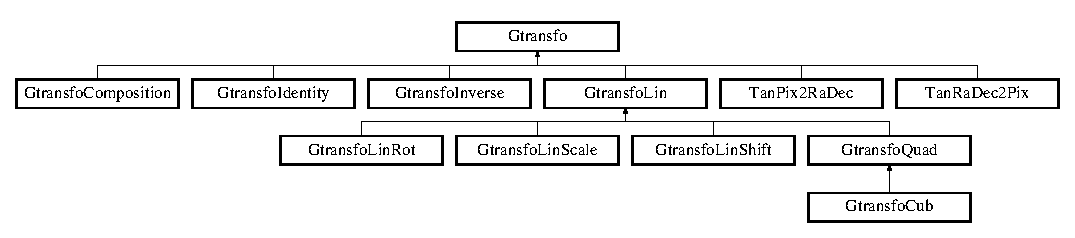
\includegraphics[height=2.7451cm]{class_gtransfo}
\end{center}
\end{figure}
\subsubsection*{Public Methods}
\begin{CompactItemize}
\item 
\index{apply@{apply}!Gtransfo@{Gtransfo}}\index{Gtransfo@{Gtransfo}!apply@{apply}}
virtual void {\bf apply} (const double Xin, const double Yin, double \&Xout, double \&Yout) const=0\label{class_gtransfo_a0}

\item 
\index{apply@{apply}!Gtransfo@{Gtransfo}}\index{Gtransfo@{Gtransfo}!apply@{apply}}
void {\bf apply} (const {\bf Point} \&Pin, {\bf Point} \&Pout) const\label{class_gtransfo_a1}

\begin{CompactList}\small\item\em applies the tranfo to Pin and writes into Pout. Is indeed virtual.\item\end{CompactList}\item 
\index{apply@{apply}!Gtransfo@{Gtransfo}}\index{Gtransfo@{Gtransfo}!apply@{apply}}
{\bf Point} {\bf apply} (const {\bf Point} \&Pin) const\label{class_gtransfo_a2}

\item 
\index{dump@{dump}!Gtransfo@{Gtransfo}}\index{Gtransfo@{Gtransfo}!dump@{dump}}
virtual void {\bf dump} (ostream \&stream=cout) const=0\label{class_gtransfo_a3}

\begin{CompactList}\small\item\em dumps the transfo coefficients to stream.\item\end{CompactList}\item 
virtual double {\bf fit} (const Star\-Match\-List \&List, const Gtransfo $\ast$Prior\-Transfo=NULL, const Gtransfo $\ast$Posterior\-Transfo=NULL)=0
\begin{CompactList}\small\item\em fits a transfo to a list of star pairs (p1,p2).\item\end{CompactList}\item 
\index{operator()@{operator()}!Gtransfo@{Gtransfo}}\index{Gtransfo@{Gtransfo}!operator()@{operator()}}
{\bf Point} {\bf operator()} (const {\bf Point} \&In) const\label{class_gtransfo_a5}

\begin{CompactList}\small\item\em allows to write My\-Transfo(My\-Star).\item\end{CompactList}\item 
\index{ReduceCompo@{ReduceCompo}!Gtransfo@{Gtransfo}}\index{Gtransfo@{Gtransfo}!ReduceCompo@{Reduce\-Compo}}
virtual Gtransfo$\ast$ {\bf Reduce\-Compo} (const Gtransfo $\ast$Right) const\label{class_gtransfo_a6}

\begin{CompactList}\small\item\em allow composition of transformations regardless of their actual types.see {\bf Gtransfo\-Compose}() {\rm (p.\,\pageref{gtransfo_h_a1})} for a user callable entry.\item\end{CompactList}\item 
\index{Clone@{Clone}!Gtransfo@{Gtransfo}}\index{Gtransfo@{Gtransfo}!Clone@{Clone}}
virtual Gtransfo$\ast$ {\bf Clone} () const=0\label{class_gtransfo_a7}

\begin{CompactList}\small\item\em returns a copy (allocated by new) of the transformation.\item\end{CompactList}\item 
\index{Jacobian@{Jacobian}!Gtransfo@{Gtransfo}}\index{Gtransfo@{Gtransfo}!Jacobian@{Jacobian}}
virtual double {\bf Jacobian} (const double x, const double y) const\label{class_gtransfo_a8}

\begin{CompactList}\small\item\em returns the local jacobian.\item\end{CompactList}\item 
virtual void {\bf Derivative} (const {\bf Point} \&Where, {\bf Gtransfo\-Lin} \&Der, const double Step=0.01) const
\begin{CompactList}\small\item\em Computes the local Derivative of a transfo. Step is used for numerical derivation.\item\end{CompactList}\item 
\index{LinearApproximation@{LinearApproximation}!Gtransfo@{Gtransfo}}\index{Gtransfo@{Gtransfo}!LinearApproximation@{Linear\-Approximation}}
virtual {\bf Gtransfo\-Lin} {\bf Linear\-Approximation} (const {\bf Point} \&Where, const double step=0.01) const\label{class_gtransfo_a10}

\begin{CompactList}\small\item\em linear (local) approximation.\item\end{CompactList}\item 
\index{TransformErrors@{TransformErrors}!Gtransfo@{Gtransfo}}\index{Gtransfo@{Gtransfo}!TransformErrors@{Transform\-Errors}}
virtual void {\bf Transform\-Errors} (const {\bf Point} \&Where, const double $\ast$VIn, double $\ast$VOut) const\label{class_gtransfo_a11}

\begin{CompactList}\small\item\em transform errors (represented as double[3] in order V(xx),V(yy),Cov(xy)).\item\end{CompactList}\item 
virtual Gtransfo$\ast$ {\bf Inverse\-Transfo} (const double Precision, const {\bf Frame} \&Region) const
\begin{CompactList}\small\item\em returns an inverse transfo.\item\end{CompactList}\item 
virtual Gtransfo$\ast$ {\bf Rough\-Inverse} (const {\bf Frame} \&Region) const
\begin{CompactList}\small\item\em Rough inverse.\item\end{CompactList}\item 
\index{Npar@{Npar}!Gtransfo@{Gtransfo}}\index{Gtransfo@{Gtransfo}!Npar@{Npar}}
virtual int {\bf Npar} () const\label{class_gtransfo_a14}

\begin{CompactList}\small\item\em returns the number of parameters (to compute chi2's).\item\end{CompactList}\item 
\index{~Gtransfo@{$\sim$Gtransfo}!Gtransfo@{Gtransfo}}\index{Gtransfo@{Gtransfo}!~Gtransfo@{$\sim$Gtransfo}}
virtual {\bf $\sim$Gtransfo} ()\label{class_gtransfo_a15}

\end{CompactItemize}


\subsubsection{Detailed Description}
a virtual (interface) class for geometric transformations.

We implement here One Gtransfo interface class, and actual derived classes. Composition in the usual (mathematical) sense is provided using {\bf Gtransfo\-Compose}() {\rm (p.\,\pageref{gtransfo_h_a1})}, and some classes (e.g. {\bf Gtransfo\-Lin} {\rm (p.\,\pageref{class_gtransfolin})}) handle a $\ast$ operator. Generic inversion by iteration exists, but it is at least 10 times slower than the corresponding \char`\"{}direct transformation\char`\"{}. If a transfo has an analytical inverse, then providing Inverse\-Transfo is obviously a very good idea. Before resorting to Inverse\-Transfo, consider using Star\-Match\-List::Inverse\-Transfo(). {\bf Gtransfo\-Lin::invert}() {\rm (p.\,\pageref{class_gtransfolin_a2})} and {\bf Tan\-Pix2Ra\-Dec::invert}() {\rm (p.\,\pageref{class_tanpix2radec_a7})} exist. The classes also provide derivation and linear approximation. 



\subsubsection{Member Function Documentation}
\index{Gtransfo@{Gtransfo}!Derivative@{Derivative}}
\index{Derivative@{Derivative}!Gtransfo@{Gtransfo}}
\paragraph{\setlength{\rightskip}{0pt plus 5cm}void Gtransfo::Derivative (const {\bf Point} \& {\em Where}, {\bf Gtransfo\-Lin} \& {\em Derivative}, const double {\em Step} = 0.01) const\hspace{0.3cm}{\tt  [virtual]}}\hfill\label{class_gtransfo_a9}


Computes the local Derivative of a transfo. Step is used for numerical derivation.

the Derivative is represented by a {\bf Gtransfo\-Lin} {\rm (p.\,\pageref{class_gtransfolin})}, in which (hopefully), the offset terms are zero. Derivative should  transform a vector of offsets into a vector of offsets. 

Reimplemented in {\bf Gtransfo\-Identity} {\rm (p.\,\pageref{class_gtransfoidentity_a7})}, {\bf Gtransfo\-Lin} {\rm (p.\,\pageref{class_gtransfolin_a5})}, and {\bf Gtransfo\-Quad} {\rm (p.\,\pageref{class_gtransfoquad_a9})}.\index{Gtransfo@{Gtransfo}!InverseTransfo@{InverseTransfo}}
\index{InverseTransfo@{InverseTransfo}!Gtransfo@{Gtransfo}}
\paragraph{\setlength{\rightskip}{0pt plus 5cm}Gtransfo $\ast$ Gtransfo::Inverse\-Transfo (const double {\em Precision}, const {\bf Frame} \& {\em Region}) const\hspace{0.3cm}{\tt  [virtual]}}\hfill\label{class_gtransfo_a12}


returns an inverse transfo.

Precision and Region refer to the \char`\"{}input\char`\"{} side of this,  and hence to the output side of the returned Gtransfo. 

Reimplemented in {\bf Gtransfo\-Lin} {\rm (p.\,\pageref{class_gtransfolin_a14})}, {\bf Gtransfo\-Quad} {\rm (p.\,\pageref{class_gtransfoquad_a8})}, {\bf Tan\-Pix2Ra\-Dec} {\rm (p.\,\pageref{class_tanpix2radec_a9})}, and {\bf Tan\-Ra\-Dec2Pix} {\rm (p.\,\pageref{class_tanradec2pix_a7})}.\index{Gtransfo@{Gtransfo}!RoughInverse@{RoughInverse}}
\index{RoughInverse@{RoughInverse}!Gtransfo@{Gtransfo}}
\paragraph{\setlength{\rightskip}{0pt plus 5cm}Gtransfo $\ast$ Gtransfo::Rough\-Inverse (const {\bf Frame} \& {\em Region}) const\hspace{0.3cm}{\tt  [virtual]}}\hfill\label{class_gtransfo_a13}


Rough inverse.

Stored by the numerical inverter to guess starting point  for the trials. Just here to enable overloading. 

Reimplemented in {\bf Tan\-Pix2Ra\-Dec} {\rm (p.\,\pageref{class_tanpix2radec_a8})}, and {\bf Tan\-Ra\-Dec2Pix} {\rm (p.\,\pageref{class_tanradec2pix_a6})}.\index{Gtransfo@{Gtransfo}!fit@{fit}}
\index{fit@{fit}!Gtransfo@{Gtransfo}}
\paragraph{\setlength{\rightskip}{0pt plus 5cm}double Gtransfo::fit (const Star\-Match\-List \& {\em List}, const Gtransfo $\ast$ {\em Prior\-Transfo} = NULL, const Gtransfo $\ast$ {\em Posterior\-Transfo} = NULL)\hspace{0.3cm}{\tt  [pure virtual]}}\hfill\label{class_gtransfo_a4}


fits a transfo to a list of star pairs (p1,p2).

After the fit this(Prior\-Transfo(p1)) yields approximately Posterior\-Transfo(p2). The returned value is the chi2. 

Reimplemented in {\bf Gtransfo\-Identity} {\rm (p.\,\pageref{class_gtransfoidentity_a2})}, {\bf Gtransfo\-Lin} {\rm (p.\,\pageref{class_gtransfolin_a9})}, {\bf Gtransfo\-Lin\-Shift} {\rm (p.\,\pageref{class_gtransfolinshift_a2})}, {\bf Gtransfo\-Lin\-Rot} {\rm (p.\,\pageref{class_gtransfolinrot_a2})}, {\bf Gtransfo\-Quad} {\rm (p.\,\pageref{class_gtransfoquad_a5})}, {\bf Gtransfo\-Cub} {\rm (p.\,\pageref{class_gtransfocub_a6})}, {\bf Tan\-Pix2Ra\-Dec} {\rm (p.\,\pageref{class_tanpix2radec_a17})}, and {\bf Tan\-Ra\-Dec2Pix} {\rm (p.\,\pageref{class_tanradec2pix_a10})}.

The documentation for this class was generated from the following files:\begin{CompactItemize}
\item 
{\bf gtransfo.h}\item 
gtransfo.cc\end{CompactItemize}

\subsection{Gtransfo\-Cub  Class Reference}
\label{class_gtransfocub}\index{GtransfoCub@{Gtransfo\-Cub}}
implements the cubic transformations (20 real coefficients). 


{\tt \#include $<$gtransfo.h$>$}

Inheritance diagram for Gtransfo\-Cub::\begin{figure}[H]
\begin{center}
\leavevmode
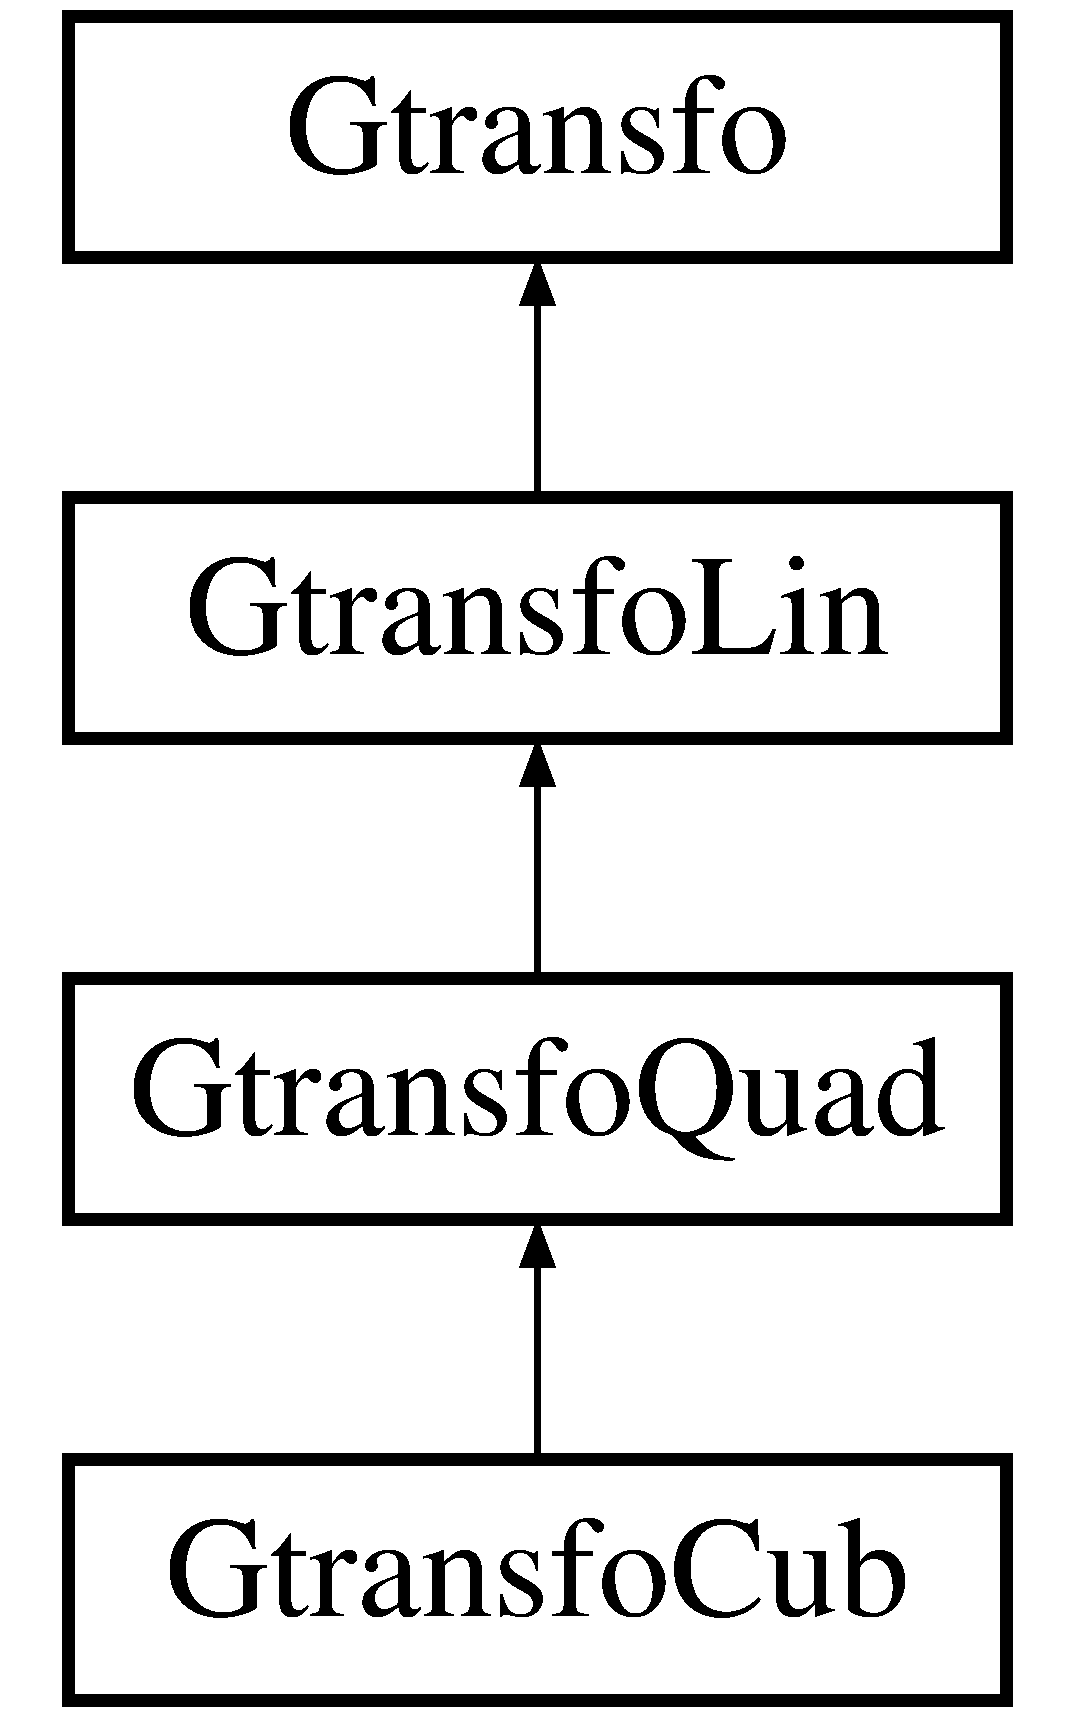
\includegraphics[height=4cm]{class_gtransfocub}
\end{center}
\end{figure}
\subsubsection*{Public Types}
\begin{CompactItemize}
\item 
enum {\bf Old\-Or\-New} \{ {\bf Old}, 
{\bf New}
 \}
\end{CompactItemize}
\subsubsection*{Public Methods}
\begin{CompactItemize}
\item 
\index{GtransfoCub@{GtransfoCub}!GtransfoCub@{Gtransfo\-Cub}}\index{GtransfoCub@{GtransfoCub}!GtransfoCub@{Gtransfo\-Cub}}
{\bf Gtransfo\-Cub} ()\label{class_gtransfocub_a0}

\begin{CompactList}\small\item\em the default constructor constructs the do-nothing transformation.\item\end{CompactList}\item 
\index{GtransfoCub@{GtransfoCub}!GtransfoCub@{Gtransfo\-Cub}}\index{GtransfoCub@{GtransfoCub}!GtransfoCub@{Gtransfo\-Cub}}
{\bf Gtransfo\-Cub} (const {\bf Gtransfo\-Lin} \&Lin)\label{class_gtransfocub_a1}

\begin{CompactList}\small\item\em upgrade a linear transfo to a cubic one.\item\end{CompactList}\item 
\index{GtransfoCub@{GtransfoCub}!GtransfoCub@{Gtransfo\-Cub}}\index{GtransfoCub@{GtransfoCub}!GtransfoCub@{Gtransfo\-Cub}}
{\bf Gtransfo\-Cub} (const {\bf Gtransfo\-Quad} \&Quad)\label{class_gtransfocub_a2}

\begin{CompactList}\small\item\em upgrade a quadratic transfo to a cubic one.\item\end{CompactList}\item 
\index{apply@{apply}!GtransfoCub@{Gtransfo\-Cub}}\index{GtransfoCub@{GtransfoCub}!apply@{apply}}
void {\bf apply} (const double Xin, const double Yin, double \&Xout, double \&Yout) const\label{class_gtransfocub_a3}

\item 
\index{apply@{apply}!GtransfoCub@{Gtransfo\-Cub}}\index{GtransfoCub@{GtransfoCub}!apply@{apply}}
{\bf Point} {\bf apply} (const {\bf Point} \&Pin)\label{class_gtransfocub_a4}

\item 
\index{dump@{dump}!GtransfoCub@{Gtransfo\-Cub}}\index{GtransfoCub@{GtransfoCub}!dump@{dump}}
void {\bf dump} (ostream \&stream=cout) const\label{class_gtransfocub_a5}

\begin{CompactList}\small\item\em dumps the transfo coefficients to stream.\item\end{CompactList}\item 
double {\bf fit} (const Star\-Match\-List \&List, const {\bf Gtransfo} $\ast$Prior\-Transfo=NULL, const {\bf Gtransfo} $\ast$Posterior\-Transfo=NULL)
\item 
\index{Clone@{Clone}!GtransfoCub@{Gtransfo\-Cub}}\index{GtransfoCub@{GtransfoCub}!Clone@{Clone}}
{\bf Gtransfo}$\ast$ {\bf Clone} () const\label{class_gtransfocub_a7}

\begin{CompactList}\small\item\em returns a copy (allocated by new) of the transformation.\item\end{CompactList}\item 
\index{ReduceCompo@{ReduceCompo}!GtransfoCub@{Gtransfo\-Cub}}\index{GtransfoCub@{GtransfoCub}!ReduceCompo@{Reduce\-Compo}}
{\bf Gtransfo}$\ast$ {\bf Reduce\-Compo} (const {\bf Gtransfo} $\ast$Right) const\label{class_gtransfocub_a8}

\begin{CompactList}\small\item\em allow composition of transformations regardless of their actual types.see {\bf Gtransfo\-Compose}() {\rm (p.\,\pageref{gtransfo_h_a1})} for a user callable entry.\item\end{CompactList}\item 
\index{dX@{dX}!GtransfoCub@{Gtransfo\-Cub}}\index{GtransfoCub@{GtransfoCub}!dX@{d\-X}}
double {\bf d\-X} () const\label{class_gtransfocub_a9}

\item 
\index{dY@{dY}!GtransfoCub@{Gtransfo\-Cub}}\index{GtransfoCub@{GtransfoCub}!dY@{d\-Y}}
double {\bf d\-Y} () const\label{class_gtransfocub_a10}

\item 
\index{A11@{A11}!GtransfoCub@{Gtransfo\-Cub}}\index{GtransfoCub@{GtransfoCub}!A11@{A11}}
double {\bf A11} () const\label{class_gtransfocub_a11}

\item 
\index{A12@{A12}!GtransfoCub@{Gtransfo\-Cub}}\index{GtransfoCub@{GtransfoCub}!A12@{A12}}
double {\bf A12} () const\label{class_gtransfocub_a12}

\item 
\index{A21@{A21}!GtransfoCub@{Gtransfo\-Cub}}\index{GtransfoCub@{GtransfoCub}!A21@{A21}}
double {\bf A21} () const\label{class_gtransfocub_a13}

\item 
\index{A22@{A22}!GtransfoCub@{Gtransfo\-Cub}}\index{GtransfoCub@{GtransfoCub}!A22@{A22}}
double {\bf A22} () const\label{class_gtransfocub_a14}

\item 
\index{A1X2@{A1X2}!GtransfoCub@{Gtransfo\-Cub}}\index{GtransfoCub@{GtransfoCub}!A1X2@{A1X2}}
double {\bf A1X2} () const\label{class_gtransfocub_a15}

\item 
\index{A1XY@{A1XY}!GtransfoCub@{Gtransfo\-Cub}}\index{GtransfoCub@{GtransfoCub}!A1XY@{A1XY}}
double {\bf A1XY} () const\label{class_gtransfocub_a16}

\item 
\index{A1Y2@{A1Y2}!GtransfoCub@{Gtransfo\-Cub}}\index{GtransfoCub@{GtransfoCub}!A1Y2@{A1Y2}}
double {\bf A1Y2} () const\label{class_gtransfocub_a17}

\item 
\index{A2X2@{A2X2}!GtransfoCub@{Gtransfo\-Cub}}\index{GtransfoCub@{GtransfoCub}!A2X2@{A2X2}}
double {\bf A2X2} () const\label{class_gtransfocub_a18}

\item 
\index{A2XY@{A2XY}!GtransfoCub@{Gtransfo\-Cub}}\index{GtransfoCub@{GtransfoCub}!A2XY@{A2XY}}
double {\bf A2XY} () const\label{class_gtransfocub_a19}

\item 
\index{A2Y2@{A2Y2}!GtransfoCub@{Gtransfo\-Cub}}\index{GtransfoCub@{GtransfoCub}!A2Y2@{A2Y2}}
double {\bf A2Y2} () const\label{class_gtransfocub_a20}

\item 
\index{A1X3@{A1X3}!GtransfoCub@{Gtransfo\-Cub}}\index{GtransfoCub@{GtransfoCub}!A1X3@{A1X3}}
double {\bf A1X3} () const\label{class_gtransfocub_a21}

\item 
\index{A1X2Y@{A1X2Y}!GtransfoCub@{Gtransfo\-Cub}}\index{GtransfoCub@{GtransfoCub}!A1X2Y@{A1X2Y}}
double {\bf A1X2Y} () const\label{class_gtransfocub_a22}

\item 
\index{A1XY2@{A1XY2}!GtransfoCub@{Gtransfo\-Cub}}\index{GtransfoCub@{GtransfoCub}!A1XY2@{A1XY2}}
double {\bf A1XY2} () const\label{class_gtransfocub_a23}

\item 
\index{A1Y3@{A1Y3}!GtransfoCub@{Gtransfo\-Cub}}\index{GtransfoCub@{GtransfoCub}!A1Y3@{A1Y3}}
double {\bf A1Y3} () const\label{class_gtransfocub_a24}

\item 
\index{A2X3@{A2X3}!GtransfoCub@{Gtransfo\-Cub}}\index{GtransfoCub@{GtransfoCub}!A2X3@{A2X3}}
double {\bf A2X3} () const\label{class_gtransfocub_a25}

\item 
\index{A2X2Y@{A2X2Y}!GtransfoCub@{Gtransfo\-Cub}}\index{GtransfoCub@{GtransfoCub}!A2X2Y@{A2X2Y}}
double {\bf A2X2Y} () const\label{class_gtransfocub_a26}

\item 
\index{A2XY2@{A2XY2}!GtransfoCub@{Gtransfo\-Cub}}\index{GtransfoCub@{GtransfoCub}!A2XY2@{A2XY2}}
double {\bf A2XY2} () const\label{class_gtransfocub_a27}

\item 
\index{A2Y3@{A2Y3}!GtransfoCub@{Gtransfo\-Cub}}\index{GtransfoCub@{GtransfoCub}!A2Y3@{A2Y3}}
double {\bf A2Y3} () const\label{class_gtransfocub_a28}

\item 
\index{GetValues@{GetValues}!GtransfoCub@{Gtransfo\-Cub}}\index{GtransfoCub@{GtransfoCub}!GetValues@{Get\-Values}}
void {\bf Get\-Values} (vector$<$ {\bf Named\-Value} $>$ \&Values, const Old\-Or\-New Which\-Names=New) const\label{class_gtransfocub_a29}

\item 
\index{SetValues@{SetValues}!GtransfoCub@{Gtransfo\-Cub}}\index{GtransfoCub@{GtransfoCub}!SetValues@{Set\-Values}}
void {\bf Set\-Values} (vector$<$ {\bf Named\-Value} $>$ \&Values)\label{class_gtransfocub_a30}

\item 
\index{Npar@{Npar}!GtransfoCub@{Gtransfo\-Cub}}\index{GtransfoCub@{GtransfoCub}!Npar@{Npar}}
int {\bf Npar} () const\label{class_gtransfocub_a31}

\begin{CompactList}\small\item\em returns the number of parameters (to compute chi2's).\item\end{CompactList}\item 
\index{Degree@{Degree}!GtransfoCub@{Gtransfo\-Cub}}\index{GtransfoCub@{GtransfoCub}!Degree@{Degree}}
virtual int {\bf Degree} () const\label{class_gtransfocub_a32}

\end{CompactItemize}
\subsubsection*{Protected Methods}
\begin{CompactItemize}
\item 
\index{identity@{identity}!GtransfoCub@{Gtransfo\-Cub}}\index{GtransfoCub@{GtransfoCub}!identity@{identity}}
void {\bf identity} ()\label{class_gtransfocub_b0}

\end{CompactItemize}
\subsubsection*{Protected Attributes}
\begin{CompactItemize}
\item 
\index{a1x3@{a1x3}!GtransfoCub@{Gtransfo\-Cub}}\index{GtransfoCub@{GtransfoCub}!a1x3@{a1x3}}
double {\bf a1x3}\label{class_gtransfocub_n0}

\item 
\index{a1x2y@{a1x2y}!GtransfoCub@{Gtransfo\-Cub}}\index{GtransfoCub@{GtransfoCub}!a1x2y@{a1x2y}}
double {\bf a1x2y}\label{class_gtransfocub_n1}

\item 
\index{a1xy2@{a1xy2}!GtransfoCub@{Gtransfo\-Cub}}\index{GtransfoCub@{GtransfoCub}!a1xy2@{a1xy2}}
double {\bf a1xy2}\label{class_gtransfocub_n2}

\item 
\index{a1y3@{a1y3}!GtransfoCub@{Gtransfo\-Cub}}\index{GtransfoCub@{GtransfoCub}!a1y3@{a1y3}}
double {\bf a1y3}\label{class_gtransfocub_n3}

\item 
\index{a2x3@{a2x3}!GtransfoCub@{Gtransfo\-Cub}}\index{GtransfoCub@{GtransfoCub}!a2x3@{a2x3}}
double {\bf a2x3}\label{class_gtransfocub_n4}

\item 
\index{a2x2y@{a2x2y}!GtransfoCub@{Gtransfo\-Cub}}\index{GtransfoCub@{GtransfoCub}!a2x2y@{a2x2y}}
double {\bf a2x2y}\label{class_gtransfocub_n5}

\item 
\index{a2xy2@{a2xy2}!GtransfoCub@{Gtransfo\-Cub}}\index{GtransfoCub@{GtransfoCub}!a2xy2@{a2xy2}}
double {\bf a2xy2}\label{class_gtransfocub_n6}

\item 
\index{a2y3@{a2y3}!GtransfoCub@{Gtransfo\-Cub}}\index{GtransfoCub@{GtransfoCub}!a2y3@{a2y3}}
double {\bf a2y3}\label{class_gtransfocub_n7}

\end{CompactItemize}
\subsubsection*{Friends}
\begin{CompactItemize}
\item 
\index{operator *@{operator $\ast$}!GtransfoCub@{Gtransfo\-Cub}}\index{GtransfoCub@{GtransfoCub}!operator *@{operator $\ast$}}
Gtransfo\-Cub {\bf operator $\ast$} (const Gtransfo\-Cub \&L, const {\bf Gtransfo\-Lin} \&R)\label{class_gtransfocub_l0}

\begin{CompactList}\small\item\em Cub$\ast$Lin.\item\end{CompactList}\item 
\index{operator *@{operator $\ast$}!GtransfoCub@{Gtransfo\-Cub}}\index{GtransfoCub@{GtransfoCub}!operator *@{operator $\ast$}}
Gtransfo\-Cub {\bf operator $\ast$} (const {\bf Gtransfo\-Lin} \&L, const Gtransfo\-Cub \&R)\label{class_gtransfocub_l1}

\begin{CompactList}\small\item\em Lin$\ast$Cub.\item\end{CompactList}\end{CompactItemize}


\subsubsection{Detailed Description}
implements the cubic transformations (20 real coefficients).



\subsubsection{Member Function Documentation}
\index{GtransfoCub@{Gtransfo\-Cub}!fit@{fit}}
\index{fit@{fit}!GtransfoCub@{Gtransfo\-Cub}}
\paragraph{\setlength{\rightskip}{0pt plus 5cm}double Gtransfo\-Cub::fit (const Star\-Match\-List \& {\em List}, const {\bf Gtransfo} $\ast$ {\em Prior\-Transfo} = NULL, const {\bf Gtransfo} $\ast$ {\em Posterior\-Transfo} = NULL)\hspace{0.3cm}{\tt  [virtual]}}\hfill\label{class_gtransfocub_a6}


fits a transfo to a list of star pairs (p1,p2). After the fit this(Prior\-Transfo(p1)) yields approximately p2. The returned value is the chi2. 

Reimplemented from {\bf Gtransfo\-Quad} {\rm (p.\,\pageref{class_gtransfoquad_a5})}.

The documentation for this class was generated from the following file:\begin{CompactItemize}
\item 
{\bf gtransfo.h}\end{CompactItemize}

\subsection{Gtransfo\-Identity  Class Reference}
\label{class_gtransfoidentity}\index{GtransfoIdentity@{Gtransfo\-Identity}}
A do-nothing transformation. It anyway has dummy routines to mimick a GTransfo. 


{\tt \#include $<$gtransfo.h$>$}

Inheritance diagram for Gtransfo\-Identity::\begin{figure}[H]
\begin{center}
\leavevmode
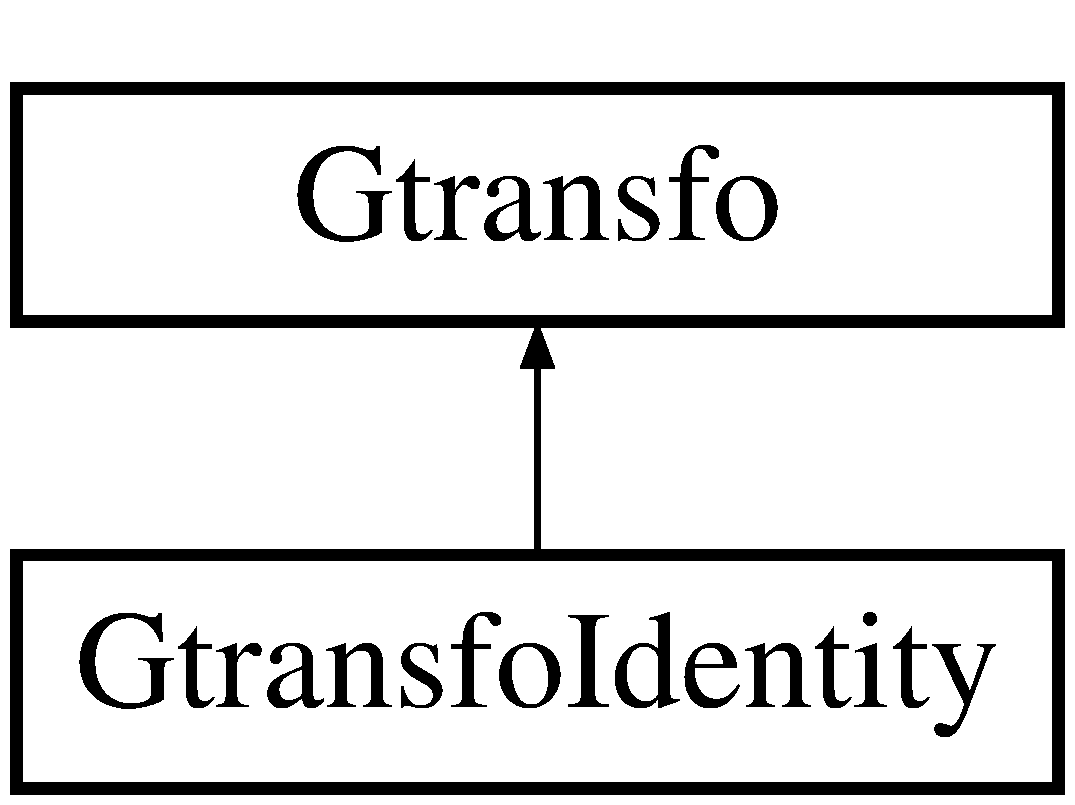
\includegraphics[height=2cm]{class_gtransfoidentity}
\end{center}
\end{figure}
\subsubsection*{Public Methods}
\begin{CompactItemize}
\item 
\index{GtransfoIdentity@{GtransfoIdentity}!GtransfoIdentity@{Gtransfo\-Identity}}\index{GtransfoIdentity@{GtransfoIdentity}!GtransfoIdentity@{Gtransfo\-Identity}}
{\bf Gtransfo\-Identity} ()\label{class_gtransfoidentity_a0}

\begin{CompactList}\small\item\em constructor.\item\end{CompactList}\item 
\index{apply@{apply}!GtransfoIdentity@{Gtransfo\-Identity}}\index{GtransfoIdentity@{GtransfoIdentity}!apply@{apply}}
void {\bf apply} (const double Xin, const double Yin, double \&Xout, double \&Yout) const\label{class_gtransfoidentity_a1}

\begin{CompactList}\small\item\em Xout = Xin; Yout = Yin !\item\end{CompactList}\item 
double {\bf fit} (const Star\-Match\-List \&List, const {\bf Gtransfo} $\ast$Prior\-Transfo=NULL, const {\bf Gtransfo} $\ast$Posterior\-Transfo=NULL)
\begin{CompactList}\small\item\em fits a transfo to a list of star pairs (p1,p2).\item\end{CompactList}\item 
\index{ReduceCompo@{ReduceCompo}!GtransfoIdentity@{Gtransfo\-Identity}}\index{GtransfoIdentity@{GtransfoIdentity}!ReduceCompo@{Reduce\-Compo}}
{\bf Gtransfo}$\ast$ {\bf Reduce\-Compo} (const {\bf Gtransfo} $\ast$Right) const\label{class_gtransfoidentity_a3}

\begin{CompactList}\small\item\em allow composition of transformations regardless of their actual types.see {\bf Gtransfo\-Compose}() {\rm (p.\,\pageref{gtransfo_h_a1})} for a user callable entry.\item\end{CompactList}\item 
\index{dump@{dump}!GtransfoIdentity@{Gtransfo\-Identity}}\index{GtransfoIdentity@{GtransfoIdentity}!dump@{dump}}
void {\bf dump} (ostream \&stream=cout) const\label{class_gtransfoidentity_a4}

\begin{CompactList}\small\item\em dumps the transfo coefficients to stream.\item\end{CompactList}\item 
\index{Npar@{Npar}!GtransfoIdentity@{Gtransfo\-Identity}}\index{GtransfoIdentity@{GtransfoIdentity}!Npar@{Npar}}
int {\bf Npar} () const\label{class_gtransfoidentity_a5}

\begin{CompactList}\small\item\em returns the number of parameters (to compute chi2's).\item\end{CompactList}\item 
\index{Clone@{Clone}!GtransfoIdentity@{Gtransfo\-Identity}}\index{GtransfoIdentity@{GtransfoIdentity}!Clone@{Clone}}
{\bf Gtransfo}$\ast$ {\bf Clone} () const\label{class_gtransfoidentity_a6}

\begin{CompactList}\small\item\em returns a copy (allocated by new) of the transformation.\item\end{CompactList}\item 
void {\bf Derivative} (const {\bf Point} \&Where, {\bf Gtransfo\-Lin} \&Derivative, const double Step=0.01) const
\begin{CompactList}\small\item\em Computes the local Derivative of a transfo. Step is used for numerical derivation.\item\end{CompactList}\item 
\index{LinearApproximation@{LinearApproximation}!GtransfoIdentity@{Gtransfo\-Identity}}\index{GtransfoIdentity@{GtransfoIdentity}!LinearApproximation@{Linear\-Approximation}}
virtual {\bf Gtransfo\-Lin} {\bf Linear\-Approximation} (const {\bf Point} \&Where, const double Step=0.01) const\label{class_gtransfoidentity_a8}

\begin{CompactList}\small\item\em linear approximation.\item\end{CompactList}\end{CompactItemize}


\subsubsection{Detailed Description}
A do-nothing transformation. It anyway has dummy routines to mimick a GTransfo.



\subsubsection{Member Function Documentation}
\index{GtransfoIdentity@{Gtransfo\-Identity}!Derivative@{Derivative}}
\index{Derivative@{Derivative}!GtransfoIdentity@{Gtransfo\-Identity}}
\paragraph{\setlength{\rightskip}{0pt plus 5cm}void Gtransfo\-Identity::Derivative (const {\bf Point} \& {\em Where}, {\bf Gtransfo\-Lin} \& {\em Derivative}, const double {\em Step} = 0.01) const\hspace{0.3cm}{\tt  [virtual]}}\hfill\label{class_gtransfoidentity_a7}


Computes the local Derivative of a transfo. Step is used for numerical derivation.

the Derivative is represented by a {\bf Gtransfo\-Lin} {\rm (p.\,\pageref{class_gtransfolin})}, in which (hopefully), the offset terms are zero. Derivative should  transform a vector of offsets into a vector of offsets. 

Reimplemented from {\bf Gtransfo} {\rm (p.\,\pageref{class_gtransfo_a9})}.\index{GtransfoIdentity@{Gtransfo\-Identity}!fit@{fit}}
\index{fit@{fit}!GtransfoIdentity@{Gtransfo\-Identity}}
\paragraph{\setlength{\rightskip}{0pt plus 5cm}double Gtransfo\-Identity::fit (const Star\-Match\-List \& {\em List}, const {\bf Gtransfo} $\ast$ {\em Prior\-Transfo} = NULL, const {\bf Gtransfo} $\ast$ {\em Posterior\-Transfo} = NULL)\hspace{0.3cm}{\tt  [inline, virtual]}}\hfill\label{class_gtransfoidentity_a2}


fits a transfo to a list of star pairs (p1,p2).

After the fit this(Prior\-Transfo(p1)) yields approximately Posterior\-Transfo(p2). The returned value is the chi2. 

Reimplemented from {\bf Gtransfo} {\rm (p.\,\pageref{class_gtransfo_a4})}.

The documentation for this class was generated from the following file:\begin{CompactItemize}
\item 
{\bf gtransfo.h}\end{CompactItemize}

\subsection{Gtransfo\-Lin  Class Reference}
\label{class_gtransfolin}\index{GtransfoLin@{Gtransfo\-Lin}}
implements the linear transformations (6 real coefficients). 


{\tt \#include $<$gtransfo.h$>$}

Inheritance diagram for Gtransfo\-Lin::\begin{figure}[H]
\begin{center}
\leavevmode
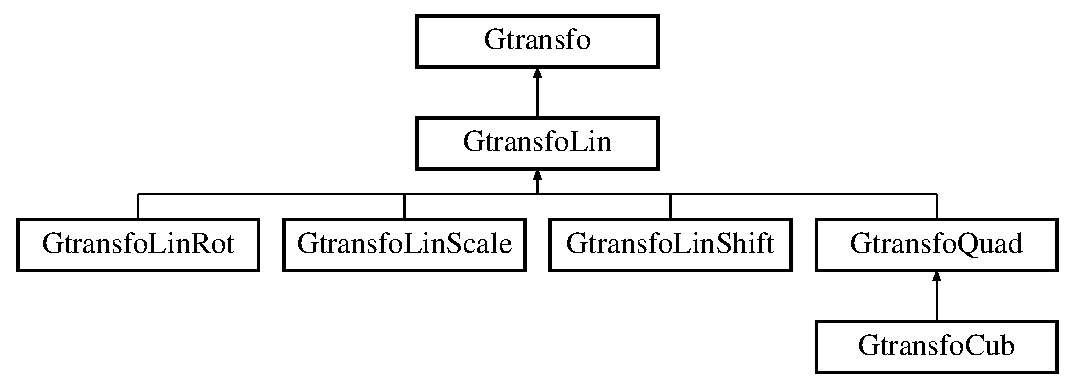
\includegraphics[height=4cm]{class_gtransfolin}
\end{center}
\end{figure}
\subsubsection*{Public Methods}
\begin{CompactItemize}
\item 
\index{GtransfoLin@{GtransfoLin}!GtransfoLin@{Gtransfo\-Lin}}\index{GtransfoLin@{GtransfoLin}!GtransfoLin@{Gtransfo\-Lin}}
{\bf Gtransfo\-Lin} ()\label{class_gtransfolin_a0}

\begin{CompactList}\small\item\em the default constructor constructs the do-nothing transformation.\item\end{CompactList}\item 
\index{operator *@{operator $\ast$}!GtransfoLin@{Gtransfo\-Lin}}\index{GtransfoLin@{GtransfoLin}!operator *@{operator $\ast$}}
Gtransfo\-Lin {\bf operator $\ast$} (const Gtransfo\-Lin \&T2) const\label{class_gtransfolin_a1}

\begin{CompactList}\small\item\em enables to combine linear tranformations: T1=T2$\ast$T3 is legal.\item\end{CompactList}\item 
\index{invert@{invert}!GtransfoLin@{Gtransfo\-Lin}}\index{GtransfoLin@{GtransfoLin}!invert@{invert}}
Gtransfo\-Lin {\bf invert} () const\label{class_gtransfolin_a2}

\begin{CompactList}\small\item\em returns the inverse: T1 = T2.invert();.\item\end{CompactList}\item 
\index{apply@{apply}!GtransfoLin@{Gtransfo\-Lin}}\index{GtransfoLin@{GtransfoLin}!apply@{apply}}
void {\bf apply} (const double Xin, const double Yin, double \&Xout, double \&Yout) const\label{class_gtransfolin_a3}

\item 
\index{Determinant@{Determinant}!GtransfoLin@{Gtransfo\-Lin}}\index{GtransfoLin@{GtransfoLin}!Determinant@{Determinant}}
double {\bf Determinant} () const\label{class_gtransfolin_a4}

\item 
void {\bf Derivative} (const {\bf Point} \&Where, Gtransfo\-Lin \&Derivative, const double Step=0.01) const
\begin{CompactList}\small\item\em Computes the local Derivative of a transfo. Step is used for numerical derivation.\item\end{CompactList}\item 
\index{LinearApproximation@{LinearApproximation}!GtransfoLin@{Gtransfo\-Lin}}\index{GtransfoLin@{GtransfoLin}!LinearApproximation@{Linear\-Approximation}}
Gtransfo\-Lin {\bf Linear\-Approximation} (const {\bf Point} \&Where, const double step=0.01) const\label{class_gtransfolin_a6}

\begin{CompactList}\small\item\em linear (local) approximation.\item\end{CompactList}\item 
\index{apply@{apply}!GtransfoLin@{Gtransfo\-Lin}}\index{GtransfoLin@{GtransfoLin}!apply@{apply}}
{\bf Point} {\bf apply} (const {\bf Point} \&Pin) const\label{class_gtransfolin_a7}

\item 
\index{dump@{dump}!GtransfoLin@{Gtransfo\-Lin}}\index{GtransfoLin@{GtransfoLin}!dump@{dump}}
void {\bf dump} (ostream \&stream=cout) const\label{class_gtransfolin_a8}

\begin{CompactList}\small\item\em dumps the transfo coefficients to stream.\item\end{CompactList}\item 
double {\bf fit} (const Star\-Match\-List \&List, const {\bf Gtransfo} $\ast$Prior\-Transfo=NULL, const {\bf Gtransfo} $\ast$Posterior\-Transfo=NULL)
\begin{CompactList}\small\item\em fits a transfo to a list of star pairs (p1,p2).\item\end{CompactList}\item 
\index{GtransfoLin@{GtransfoLin}!GtransfoLin@{Gtransfo\-Lin}}\index{GtransfoLin@{GtransfoLin}!GtransfoLin@{Gtransfo\-Lin}}
{\bf Gtransfo\-Lin} (double ox, double oy, double aa11, double aa12, double aa21, double aa22)\label{class_gtransfolin_a10}

\begin{CompactList}\small\item\em the constructor that enables to set all parameters independently. Not very useful.\item\end{CompactList}\item 
\index{GtransfoLin@{GtransfoLin}!GtransfoLin@{Gtransfo\-Lin}}\index{GtransfoLin@{GtransfoLin}!GtransfoLin@{Gtransfo\-Lin}}
{\bf Gtransfo\-Lin} (const {\bf Gtransfo\-Identity} \&T)\label{class_gtransfolin_a11}

\begin{CompactList}\small\item\em Handy converter:.\item\end{CompactList}\item 
\index{Clone@{Clone}!GtransfoLin@{Gtransfo\-Lin}}\index{GtransfoLin@{GtransfoLin}!Clone@{Clone}}
{\bf Gtransfo}$\ast$ {\bf Clone} () const\label{class_gtransfolin_a12}

\begin{CompactList}\small\item\em returns a copy (allocated by new) of the transformation.\item\end{CompactList}\item 
\index{ReduceCompo@{ReduceCompo}!GtransfoLin@{Gtransfo\-Lin}}\index{GtransfoLin@{GtransfoLin}!ReduceCompo@{Reduce\-Compo}}
{\bf Gtransfo}$\ast$ {\bf Reduce\-Compo} (const {\bf Gtransfo} $\ast$Right) const\label{class_gtransfolin_a13}

\begin{CompactList}\small\item\em allow composition of transformations regardless of their actual types.see {\bf Gtransfo\-Compose}() {\rm (p.\,\pageref{gtransfo_h_a1})} for a user callable entry.\item\end{CompactList}\item 
{\bf Gtransfo}$\ast$ {\bf Inverse\-Transfo} (const double Precision, const {\bf Frame} \&Region) const
\begin{CompactList}\small\item\em returns an inverse transfo.\item\end{CompactList}\item 
\index{A11@{A11}!GtransfoLin@{Gtransfo\-Lin}}\index{GtransfoLin@{GtransfoLin}!A11@{A11}}
double {\bf A11} () const\label{class_gtransfolin_a15}

\item 
\index{A12@{A12}!GtransfoLin@{Gtransfo\-Lin}}\index{GtransfoLin@{GtransfoLin}!A12@{A12}}
double {\bf A12} () const\label{class_gtransfolin_a16}

\item 
\index{A21@{A21}!GtransfoLin@{Gtransfo\-Lin}}\index{GtransfoLin@{GtransfoLin}!A21@{A21}}
double {\bf A21} () const\label{class_gtransfolin_a17}

\item 
\index{A22@{A22}!GtransfoLin@{Gtransfo\-Lin}}\index{GtransfoLin@{GtransfoLin}!A22@{A22}}
double {\bf A22} () const\label{class_gtransfolin_a18}

\item 
\index{dX@{dX}!GtransfoLin@{Gtransfo\-Lin}}\index{GtransfoLin@{GtransfoLin}!dX@{d\-X}}
double {\bf d\-X} () const\label{class_gtransfolin_a19}

\item 
\index{dY@{dY}!GtransfoLin@{Gtransfo\-Lin}}\index{GtransfoLin@{GtransfoLin}!dY@{d\-Y}}
double {\bf d\-Y} () const\label{class_gtransfolin_a20}

\item 
\index{Npar@{Npar}!GtransfoLin@{Gtransfo\-Lin}}\index{GtransfoLin@{GtransfoLin}!Npar@{Npar}}
virtual int {\bf Npar} () const\label{class_gtransfolin_a21}

\begin{CompactList}\small\item\em returns the number of parameters (to compute chi2's).\item\end{CompactList}\item 
\index{Degree@{Degree}!GtransfoLin@{Gtransfo\-Lin}}\index{GtransfoLin@{GtransfoLin}!Degree@{Degree}}
virtual int {\bf Degree} () const\label{class_gtransfolin_a22}

\end{CompactItemize}
\subsubsection*{Protected Methods}
\begin{CompactItemize}
\item 
\index{identity@{identity}!GtransfoLin@{Gtransfo\-Lin}}\index{GtransfoLin@{GtransfoLin}!identity@{identity}}
void {\bf identity} ()\label{class_gtransfolin_b0}

\end{CompactItemize}
\subsubsection*{Protected Attributes}
\begin{CompactItemize}
\item 
\index{dx@{dx}!GtransfoLin@{Gtransfo\-Lin}}\index{GtransfoLin@{GtransfoLin}!dx@{dx}}
double {\bf dx}\label{class_gtransfolin_n0}

\item 
\index{dy@{dy}!GtransfoLin@{Gtransfo\-Lin}}\index{GtransfoLin@{GtransfoLin}!dy@{dy}}
double {\bf dy}\label{class_gtransfolin_n1}

\item 
\index{a11@{a11}!GtransfoLin@{Gtransfo\-Lin}}\index{GtransfoLin@{GtransfoLin}!a11@{a11}}
double {\bf a11}\label{class_gtransfolin_n2}

\item 
\index{a12@{a12}!GtransfoLin@{Gtransfo\-Lin}}\index{GtransfoLin@{GtransfoLin}!a12@{a12}}
double {\bf a12}\label{class_gtransfolin_n3}

\item 
\index{a21@{a21}!GtransfoLin@{Gtransfo\-Lin}}\index{GtransfoLin@{GtransfoLin}!a21@{a21}}
double {\bf a21}\label{class_gtransfolin_n4}

\item 
\index{a22@{a22}!GtransfoLin@{Gtransfo\-Lin}}\index{GtransfoLin@{GtransfoLin}!a22@{a22}}
double {\bf a22}\label{class_gtransfolin_n5}

\end{CompactItemize}
\subsubsection*{Friends}
\begin{CompactItemize}
\item 
class {\bf Gtransfo}
\item 
class {\bf Gtransfo\-Identity}
\item 
class {\bf operator $\ast$}
\item 
class {\bf operator $\ast$}
\end{CompactItemize}


\subsubsection{Detailed Description}
implements the linear transformations (6 real coefficients).



\subsubsection{Member Function Documentation}
\index{GtransfoLin@{Gtransfo\-Lin}!Derivative@{Derivative}}
\index{Derivative@{Derivative}!GtransfoLin@{Gtransfo\-Lin}}
\paragraph{\setlength{\rightskip}{0pt plus 5cm}void Gtransfo\-Lin::Derivative (const {\bf Point} \& {\em Where}, Gtransfo\-Lin \& {\em Derivative}, const double {\em Step} = 0.01) const\hspace{0.3cm}{\tt  [virtual]}}\hfill\label{class_gtransfolin_a5}


Computes the local Derivative of a transfo. Step is used for numerical derivation.

the Derivative is represented by a Gtransfo\-Lin, in which (hopefully), the offset terms are zero. Derivative should  transform a vector of offsets into a vector of offsets. 

Reimplemented from {\bf Gtransfo} {\rm (p.\,\pageref{class_gtransfo_a9})}.

Reimplemented in {\bf Gtransfo\-Quad} {\rm (p.\,\pageref{class_gtransfoquad_a9})}.\index{GtransfoLin@{Gtransfo\-Lin}!InverseTransfo@{InverseTransfo}}
\index{InverseTransfo@{InverseTransfo}!GtransfoLin@{Gtransfo\-Lin}}
\paragraph{\setlength{\rightskip}{0pt plus 5cm}{\bf Gtransfo}$\ast$ Gtransfo\-Lin::Inverse\-Transfo (const double {\em Precision}, const {\bf Frame} \& {\em Region}) const\hspace{0.3cm}{\tt  [virtual]}}\hfill\label{class_gtransfolin_a14}


returns an inverse transfo.

Precision and Region refer to the \char`\"{}input\char`\"{} side of this,  and hence to the output side of the returned {\bf Gtransfo} {\rm (p.\,\pageref{class_gtransfo})}. 

Reimplemented from {\bf Gtransfo} {\rm (p.\,\pageref{class_gtransfo_a12})}.

Reimplemented in {\bf Gtransfo\-Quad} {\rm (p.\,\pageref{class_gtransfoquad_a8})}.\index{GtransfoLin@{Gtransfo\-Lin}!fit@{fit}}
\index{fit@{fit}!GtransfoLin@{Gtransfo\-Lin}}
\paragraph{\setlength{\rightskip}{0pt plus 5cm}double Gtransfo\-Lin::fit (const Star\-Match\-List \& {\em List}, const {\bf Gtransfo} $\ast$ {\em Prior\-Transfo} = NULL, const {\bf Gtransfo} $\ast$ {\em Posterior\-Transfo} = NULL)\hspace{0.3cm}{\tt  [virtual]}}\hfill\label{class_gtransfolin_a9}


fits a transfo to a list of star pairs (p1,p2).

After the fit this(Prior\-Transfo(p1)) yields approximately Posterior\-Transfo(p2). The returned value is the chi2. 

Reimplemented from {\bf Gtransfo} {\rm (p.\,\pageref{class_gtransfo_a4})}.

Reimplemented in {\bf Gtransfo\-Lin\-Shift} {\rm (p.\,\pageref{class_gtransfolinshift_a2})}, {\bf Gtransfo\-Lin\-Rot} {\rm (p.\,\pageref{class_gtransfolinrot_a2})}, {\bf Gtransfo\-Quad} {\rm (p.\,\pageref{class_gtransfoquad_a5})}, and {\bf Gtransfo\-Cub} {\rm (p.\,\pageref{class_gtransfocub_a6})}.

The documentation for this class was generated from the following file:\begin{CompactItemize}
\item 
{\bf gtransfo.h}\end{CompactItemize}

\subsection{Gtransfo\-Lin\-Rot  Class Reference}
\label{class_gtransfolinrot}\index{GtransfoLinRot@{Gtransfo\-Lin\-Rot}}
just here to provide a specialized constructor, and fit. 


{\tt \#include $<$gtransfo.h$>$}

Inheritance diagram for Gtransfo\-Lin\-Rot::\begin{figure}[H]
\begin{center}
\leavevmode
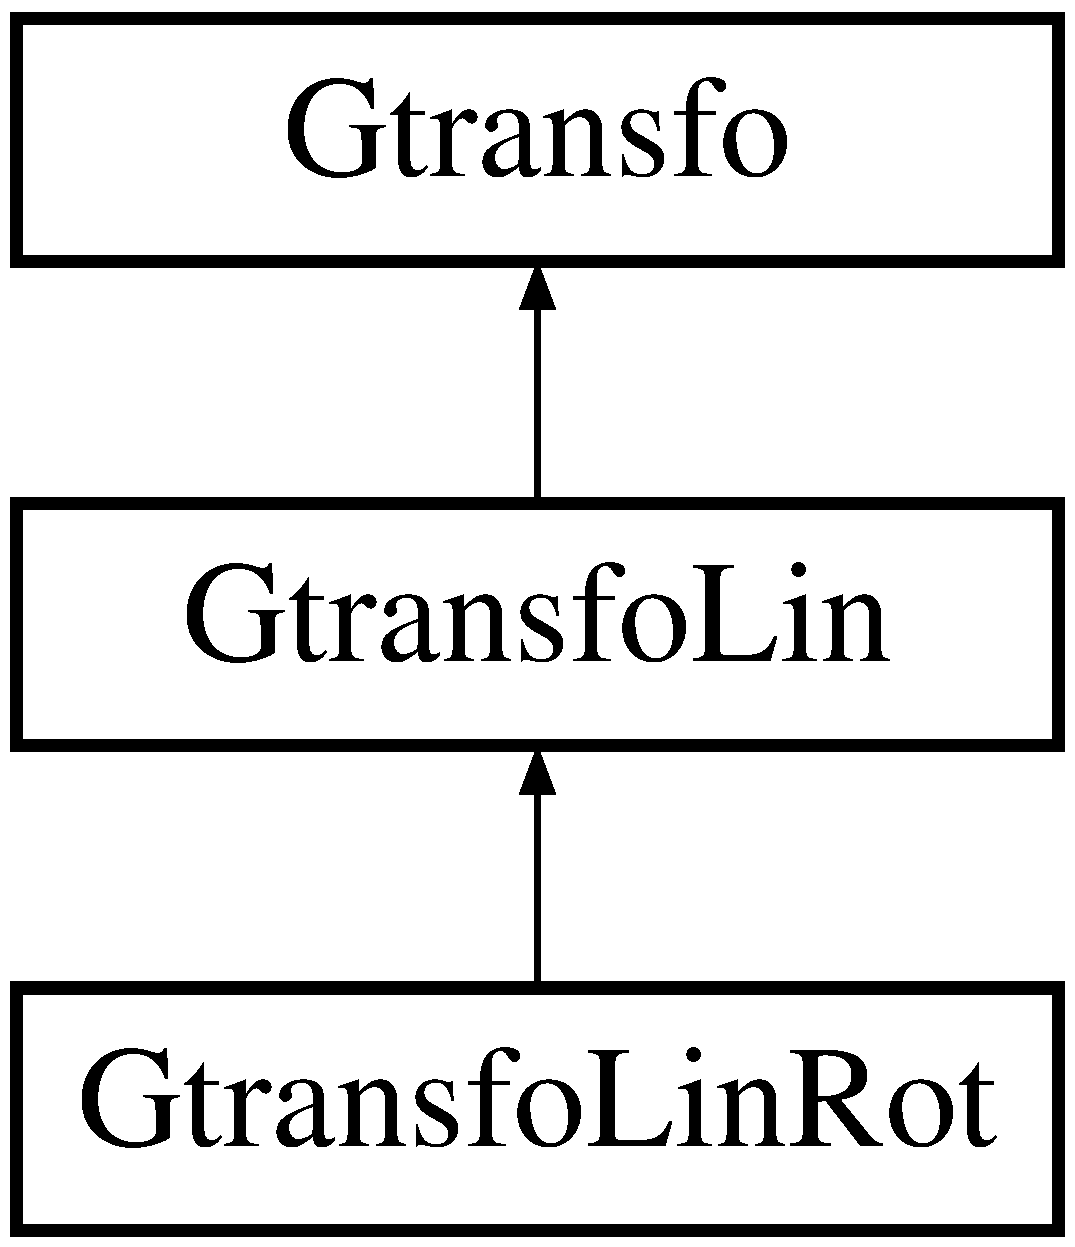
\includegraphics[height=3cm]{class_gtransfolinrot}
\end{center}
\end{figure}
\subsubsection*{Public Methods}
\begin{CompactItemize}
\item 
\index{GtransfoLinRot@{GtransfoLinRot}!GtransfoLinRot@{Gtransfo\-Lin\-Rot}}\index{GtransfoLinRot@{GtransfoLinRot}!GtransfoLinRot@{Gtransfo\-Lin\-Rot}}
{\bf Gtransfo\-Lin\-Rot} ()\label{class_gtransfolinrot_a0}

\item 
\index{GtransfoLinRot@{GtransfoLinRot}!GtransfoLinRot@{Gtransfo\-Lin\-Rot}}\index{GtransfoLinRot@{GtransfoLinRot}!GtransfoLinRot@{Gtransfo\-Lin\-Rot}}
{\bf Gtransfo\-Lin\-Rot} (const double Angle\-Rad, const {\bf Point} $\ast$Center=NULL, const double Scale\-Factor=1.0)\label{class_gtransfolinrot_a1}

\item 
double {\bf fit} (const Star\-Match\-List \&List, const {\bf Gtransfo} $\ast$Prior\-Transfo=NULL, const {\bf Gtransfo} $\ast$Posterior\-Transfo=NULL)
\begin{CompactList}\small\item\em fits a transfo to a list of star pairs (p1,p2).\item\end{CompactList}\item 
\index{Npar@{Npar}!GtransfoLinRot@{Gtransfo\-Lin\-Rot}}\index{GtransfoLinRot@{GtransfoLinRot}!Npar@{Npar}}
int {\bf Npar} () const\label{class_gtransfolinrot_a3}

\begin{CompactList}\small\item\em returns the number of parameters (to compute chi2's).\item\end{CompactList}\end{CompactItemize}


\subsubsection{Detailed Description}
just here to provide a specialized constructor, and fit.



\subsubsection{Member Function Documentation}
\index{GtransfoLinRot@{Gtransfo\-Lin\-Rot}!fit@{fit}}
\index{fit@{fit}!GtransfoLinRot@{Gtransfo\-Lin\-Rot}}
\paragraph{\setlength{\rightskip}{0pt plus 5cm}double Gtransfo\-Lin\-Rot::fit (const Star\-Match\-List \& {\em List}, const {\bf Gtransfo} $\ast$ {\em Prior\-Transfo} = NULL, const {\bf Gtransfo} $\ast$ {\em Posterior\-Transfo} = NULL)\hspace{0.3cm}{\tt  [virtual]}}\hfill\label{class_gtransfolinrot_a2}


fits a transfo to a list of star pairs (p1,p2).

After the fit this(Prior\-Transfo(p1)) yields approximately Posterior\-Transfo(p2). The returned value is the chi2. 

Reimplemented from {\bf Gtransfo\-Lin} {\rm (p.\,\pageref{class_gtransfolin_a9})}.

The documentation for this class was generated from the following file:\begin{CompactItemize}
\item 
{\bf gtransfo.h}\end{CompactItemize}

\subsection{Gtransfo\-Lin\-Scale  Class Reference}
\label{class_gtransfolinscale}\index{GtransfoLinScale@{Gtransfo\-Lin\-Scale}}
just here to provide specialized constructors. {\bf Gtransfo\-Lin} {\rm (p.\,\pageref{class_gtransfolin})} fit routine. 


{\tt \#include $<$gtransfo.h$>$}

Inheritance diagram for Gtransfo\-Lin\-Scale::\begin{figure}[H]
\begin{center}
\leavevmode
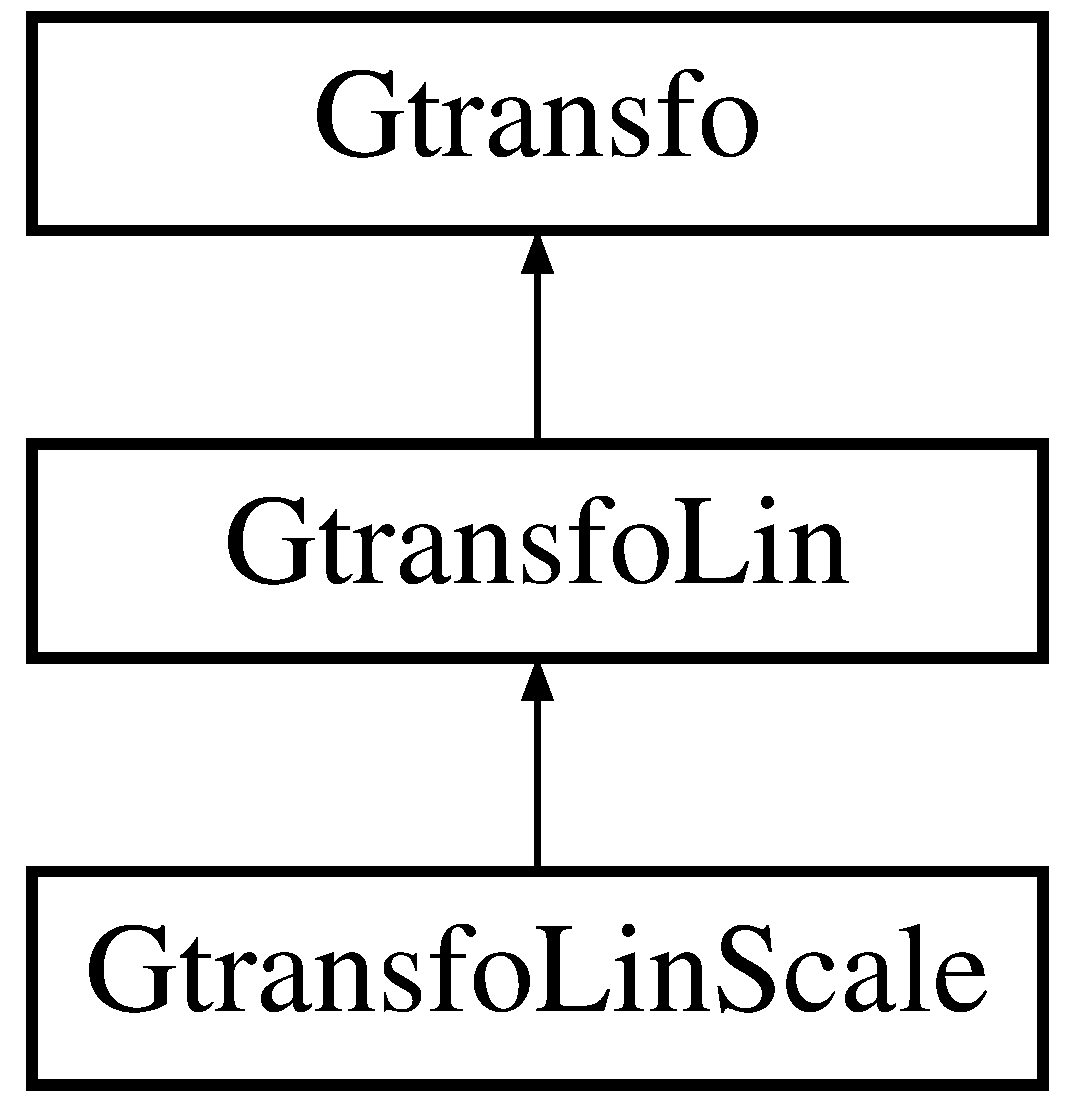
\includegraphics[height=3cm]{class_gtransfolinscale}
\end{center}
\end{figure}
\subsubsection*{Public Methods}
\begin{CompactItemize}
\item 
\index{GtransfoLinScale@{GtransfoLinScale}!GtransfoLinScale@{Gtransfo\-Lin\-Scale}}\index{GtransfoLinScale@{GtransfoLinScale}!GtransfoLinScale@{Gtransfo\-Lin\-Scale}}
{\bf Gtransfo\-Lin\-Scale} (const double Scale)\label{class_gtransfolinscale_a0}

\item 
\index{GtransfoLinScale@{GtransfoLinScale}!GtransfoLinScale@{Gtransfo\-Lin\-Scale}}\index{GtransfoLinScale@{GtransfoLinScale}!GtransfoLinScale@{Gtransfo\-Lin\-Scale}}
{\bf Gtransfo\-Lin\-Scale} (const double Scale\-X, const double Scale\-Y)\label{class_gtransfolinscale_a1}

\item 
\index{Npar@{Npar}!GtransfoLinScale@{Gtransfo\-Lin\-Scale}}\index{GtransfoLinScale@{GtransfoLinScale}!Npar@{Npar}}
int {\bf Npar} () const\label{class_gtransfolinscale_a2}

\begin{CompactList}\small\item\em returns the number of parameters (to compute chi2's).\item\end{CompactList}\end{CompactItemize}


\subsubsection{Detailed Description}
just here to provide specialized constructors. {\bf Gtransfo\-Lin} {\rm (p.\,\pageref{class_gtransfolin})} fit routine.



The documentation for this class was generated from the following file:\begin{CompactItemize}
\item 
{\bf gtransfo.h}\end{CompactItemize}

\subsection{Gtransfo\-Lin\-Shift  Class Reference}
\label{class_gtransfolinshift}\index{GtransfoLinShift@{Gtransfo\-Lin\-Shift}}
just here to provide a specialized constructor, and fit. 


{\tt \#include $<$gtransfo.h$>$}

Inheritance diagram for Gtransfo\-Lin\-Shift::\begin{figure}[H]
\begin{center}
\leavevmode
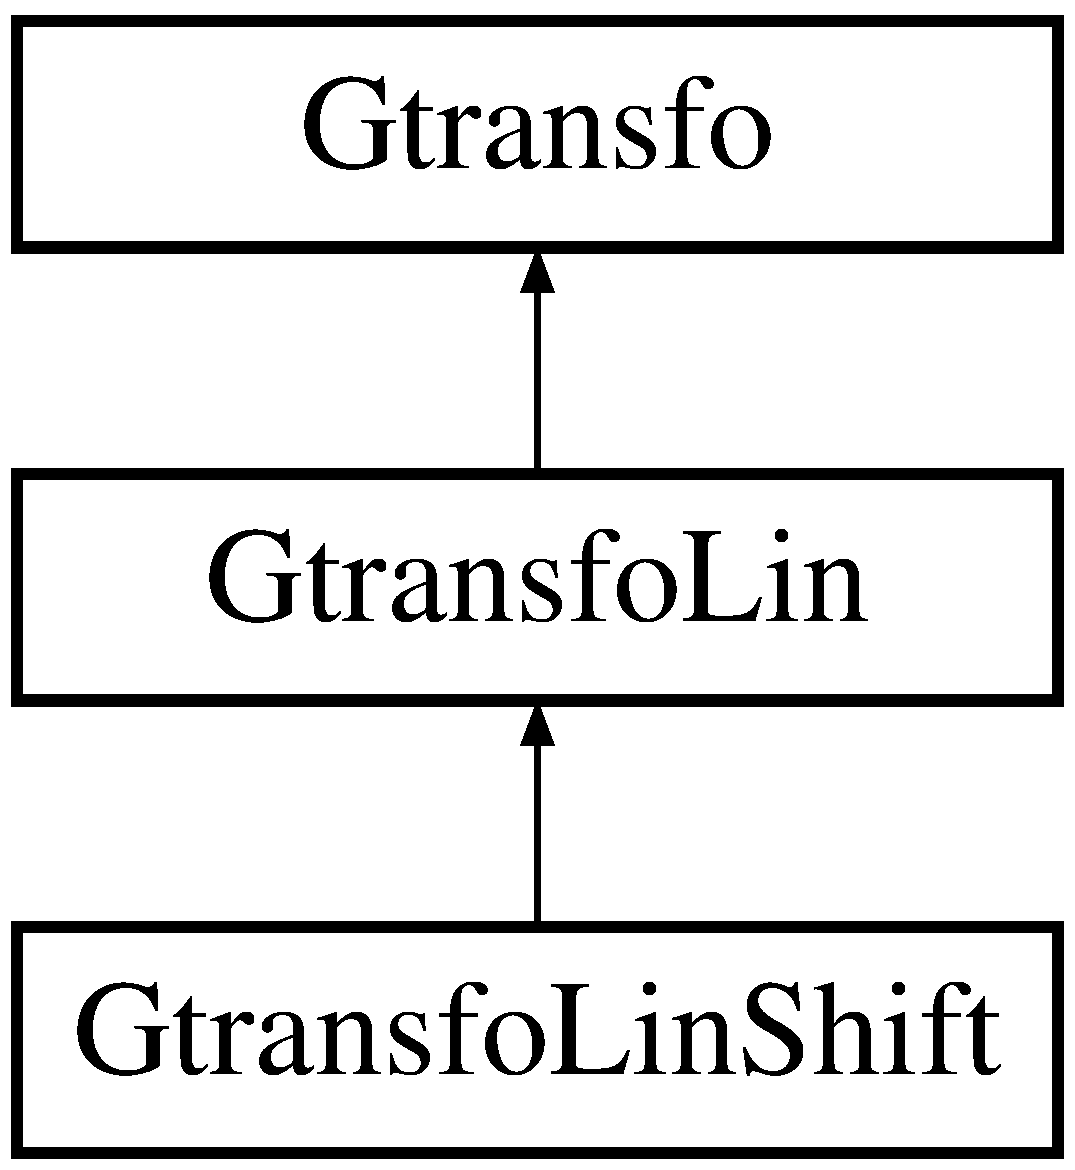
\includegraphics[height=3cm]{class_gtransfolinshift}
\end{center}
\end{figure}
\subsubsection*{Public Methods}
\begin{CompactItemize}
\item 
\index{GtransfoLinShift@{GtransfoLinShift}!GtransfoLinShift@{Gtransfo\-Lin\-Shift}}\index{GtransfoLinShift@{GtransfoLinShift}!GtransfoLinShift@{Gtransfo\-Lin\-Shift}}
{\bf Gtransfo\-Lin\-Shift} (double ox=0., double oy=0.)\label{class_gtransfolinshift_a0}

\begin{CompactList}\small\item\em Add ox and oy.\item\end{CompactList}\item 
\index{GtransfoLinShift@{GtransfoLinShift}!GtransfoLinShift@{Gtransfo\-Lin\-Shift}}\index{GtransfoLinShift@{GtransfoLinShift}!GtransfoLinShift@{Gtransfo\-Lin\-Shift}}
{\bf Gtransfo\-Lin\-Shift} (const {\bf Point} \&P)\label{class_gtransfolinshift_a1}

\item 
double {\bf fit} (const Star\-Match\-List \&List, const {\bf Gtransfo} $\ast$Prior\-Transfo=NULL, const {\bf Gtransfo} $\ast$Posterior\-Transfo=NULL)
\begin{CompactList}\small\item\em fits a transfo to a list of star pairs (p1,p2).\item\end{CompactList}\item 
\index{Npar@{Npar}!GtransfoLinShift@{Gtransfo\-Lin\-Shift}}\index{GtransfoLinShift@{GtransfoLinShift}!Npar@{Npar}}
int {\bf Npar} () const\label{class_gtransfolinshift_a3}

\begin{CompactList}\small\item\em returns the number of parameters (to compute chi2's).\item\end{CompactList}\end{CompactItemize}


\subsubsection{Detailed Description}
just here to provide a specialized constructor, and fit.



\subsubsection{Member Function Documentation}
\index{GtransfoLinShift@{Gtransfo\-Lin\-Shift}!fit@{fit}}
\index{fit@{fit}!GtransfoLinShift@{Gtransfo\-Lin\-Shift}}
\paragraph{\setlength{\rightskip}{0pt plus 5cm}double Gtransfo\-Lin\-Shift::fit (const Star\-Match\-List \& {\em List}, const {\bf Gtransfo} $\ast$ {\em Prior\-Transfo} = NULL, const {\bf Gtransfo} $\ast$ {\em Posterior\-Transfo} = NULL)\hspace{0.3cm}{\tt  [virtual]}}\hfill\label{class_gtransfolinshift_a2}


fits a transfo to a list of star pairs (p1,p2).

After the fit this(Prior\-Transfo(p1)) yields approximately Posterior\-Transfo(p2). The returned value is the chi2. 

Reimplemented from {\bf Gtransfo\-Lin} {\rm (p.\,\pageref{class_gtransfolin_a9})}.

The documentation for this class was generated from the following file:\begin{CompactItemize}
\item 
{\bf gtransfo.h}\end{CompactItemize}

\subsection{Gtransfo\-Quad  Class Reference}
\label{class_gtransfoquad}\index{GtransfoQuad@{Gtransfo\-Quad}}
implements the quadratic transformations (12 real coefficients). 


{\tt \#include $<$gtransfo.h$>$}

Inheritance diagram for Gtransfo\-Quad::\begin{figure}[H]
\begin{center}
\leavevmode
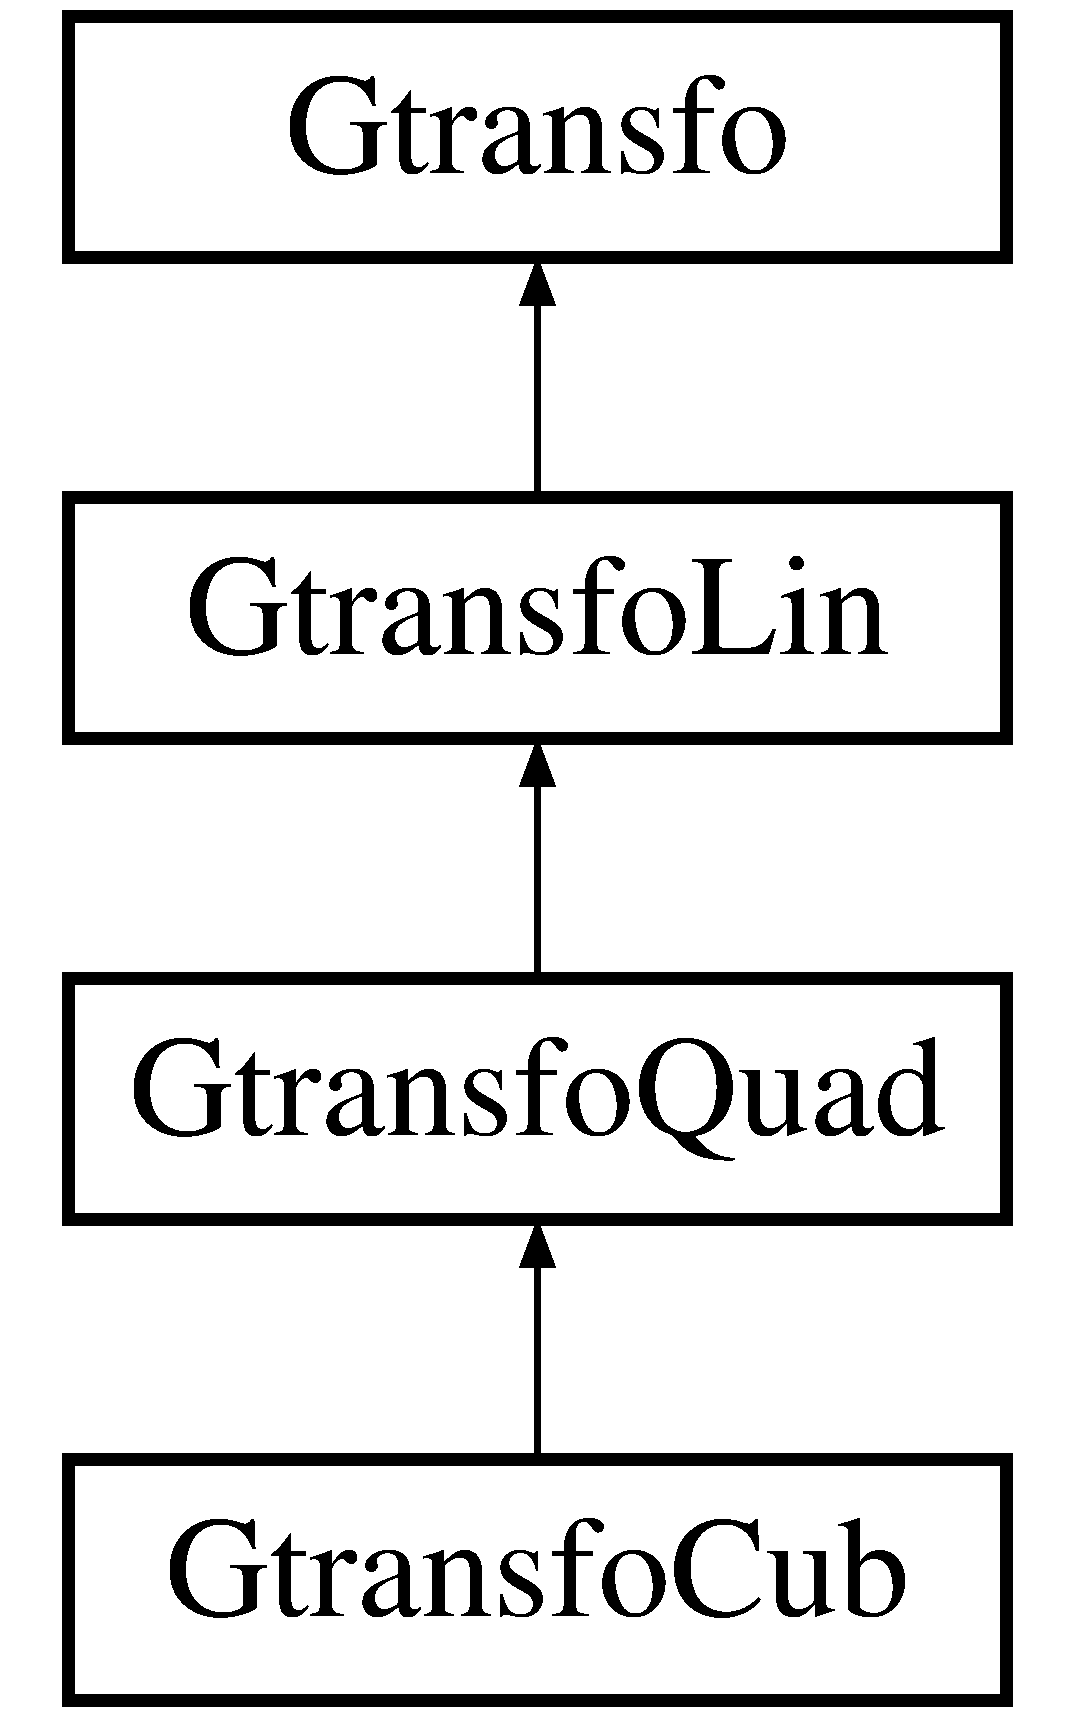
\includegraphics[height=4cm]{class_gtransfoquad}
\end{center}
\end{figure}
\subsubsection*{Public Methods}
\begin{CompactItemize}
\item 
\index{GtransfoQuad@{GtransfoQuad}!GtransfoQuad@{Gtransfo\-Quad}}\index{GtransfoQuad@{GtransfoQuad}!GtransfoQuad@{Gtransfo\-Quad}}
{\bf Gtransfo\-Quad} ()\label{class_gtransfoquad_a0}

\begin{CompactList}\small\item\em the default constructor constructs the do-nothing transformation.\item\end{CompactList}\item 
\index{GtransfoQuad@{GtransfoQuad}!GtransfoQuad@{Gtransfo\-Quad}}\index{GtransfoQuad@{GtransfoQuad}!GtransfoQuad@{Gtransfo\-Quad}}
{\bf Gtransfo\-Quad} (const {\bf Gtransfo\-Lin} \&Lin)\label{class_gtransfoquad_a1}

\begin{CompactList}\small\item\em upgrade a linear transfo to a Quad one.\item\end{CompactList}\item 
\index{operator *@{operator $\ast$}!GtransfoQuad@{Gtransfo\-Quad}}\index{GtransfoQuad@{GtransfoQuad}!operator *@{operator $\ast$}}
Gtransfo\-Quad {\bf operator $\ast$} (const {\bf Gtransfo\-Lin} \&R) const\label{class_gtransfoquad_a2}

\begin{CompactList}\small\item\em enables to combine linear tranformations: T1=T2$\ast$T3 is legal.\item\end{CompactList}\item 
\index{apply@{apply}!GtransfoQuad@{Gtransfo\-Quad}}\index{GtransfoQuad@{GtransfoQuad}!apply@{apply}}
void {\bf apply} (const double Xin, const double Yin, double \&Xout, double \&Yout) const\label{class_gtransfoquad_a3}

\item 
\index{dump@{dump}!GtransfoQuad@{Gtransfo\-Quad}}\index{GtransfoQuad@{GtransfoQuad}!dump@{dump}}
void {\bf dump} (ostream \&stream=cout) const\label{class_gtransfoquad_a4}

\begin{CompactList}\small\item\em dumps the transfo coefficients to stream.\item\end{CompactList}\item 
double {\bf fit} (const Star\-Match\-List \&List, const {\bf Gtransfo} $\ast$Prior\-Transfo=NULL, const {\bf Gtransfo} $\ast$Posterior\-Transfo=NULL)
\begin{CompactList}\small\item\em fits a transfo to a list of star pairs (p1,p2).\item\end{CompactList}\item 
\index{Clone@{Clone}!GtransfoQuad@{Gtransfo\-Quad}}\index{GtransfoQuad@{GtransfoQuad}!Clone@{Clone}}
{\bf Gtransfo}$\ast$ {\bf Clone} () const\label{class_gtransfoquad_a6}

\begin{CompactList}\small\item\em returns a copy (allocated by new) of the transformation.\item\end{CompactList}\item 
\index{ReduceCompo@{ReduceCompo}!GtransfoQuad@{Gtransfo\-Quad}}\index{GtransfoQuad@{GtransfoQuad}!ReduceCompo@{Reduce\-Compo}}
{\bf Gtransfo}$\ast$ {\bf Reduce\-Compo} (const {\bf Gtransfo} $\ast$Right) const\label{class_gtransfoquad_a7}

\begin{CompactList}\small\item\em allow composition of transformations regardless of their actual types.see {\bf Gtransfo\-Compose}() {\rm (p.\,\pageref{gtransfo_h_a1})} for a user callable entry.\item\end{CompactList}\item 
{\bf Gtransfo}$\ast$ {\bf Inverse\-Transfo} (const double Precision, const {\bf Frame} \&Region) const
\begin{CompactList}\small\item\em returns an inverse transfo.\item\end{CompactList}\item 
void {\bf Derivative} (const {\bf Point} \&Where, {\bf Gtransfo\-Lin} \&Derivative, const double Step=0.01) const
\begin{CompactList}\small\item\em Computes the local Derivative of a transfo. Step is used for numerical derivation.\item\end{CompactList}\item 
\index{LinearApproximation@{LinearApproximation}!GtransfoQuad@{Gtransfo\-Quad}}\index{GtransfoQuad@{GtransfoQuad}!LinearApproximation@{Linear\-Approximation}}
{\bf Gtransfo\-Lin} {\bf Linear\-Approximation} (const {\bf Point} \&Where, const double step=0.01) const\label{class_gtransfoquad_a10}

\begin{CompactList}\small\item\em linear (local) approximation.\item\end{CompactList}\item 
\index{A1X2@{A1X2}!GtransfoQuad@{Gtransfo\-Quad}}\index{GtransfoQuad@{GtransfoQuad}!A1X2@{A1X2}}
double {\bf A1X2} () const\label{class_gtransfoquad_a11}

\item 
\index{A1XY@{A1XY}!GtransfoQuad@{Gtransfo\-Quad}}\index{GtransfoQuad@{GtransfoQuad}!A1XY@{A1XY}}
double {\bf A1XY} () const\label{class_gtransfoquad_a12}

\item 
\index{A1Y2@{A1Y2}!GtransfoQuad@{Gtransfo\-Quad}}\index{GtransfoQuad@{GtransfoQuad}!A1Y2@{A1Y2}}
double {\bf A1Y2} () const\label{class_gtransfoquad_a13}

\item 
\index{A2X2@{A2X2}!GtransfoQuad@{Gtransfo\-Quad}}\index{GtransfoQuad@{GtransfoQuad}!A2X2@{A2X2}}
double {\bf A2X2} () const\label{class_gtransfoquad_a14}

\item 
\index{A2XY@{A2XY}!GtransfoQuad@{Gtransfo\-Quad}}\index{GtransfoQuad@{GtransfoQuad}!A2XY@{A2XY}}
double {\bf A2XY} () const\label{class_gtransfoquad_a15}

\item 
\index{A2Y2@{A2Y2}!GtransfoQuad@{Gtransfo\-Quad}}\index{GtransfoQuad@{GtransfoQuad}!A2Y2@{A2Y2}}
double {\bf A2Y2} () const\label{class_gtransfoquad_a16}

\item 
\index{Npar@{Npar}!GtransfoQuad@{Gtransfo\-Quad}}\index{GtransfoQuad@{GtransfoQuad}!Npar@{Npar}}
int {\bf Npar} () const\label{class_gtransfoquad_a17}

\begin{CompactList}\small\item\em returns the number of parameters (to compute chi2's).\item\end{CompactList}\item 
\index{Degree@{Degree}!GtransfoQuad@{Gtransfo\-Quad}}\index{GtransfoQuad@{GtransfoQuad}!Degree@{Degree}}
virtual int {\bf Degree} () const\label{class_gtransfoquad_a18}

\item 
\index{GtransfoQuad@{GtransfoQuad}!GtransfoQuad@{Gtransfo\-Quad}}\index{GtransfoQuad@{GtransfoQuad}!GtransfoQuad@{Gtransfo\-Quad}}
{\bf Gtransfo\-Quad} (double ox, double oy, double aa11, double aa12, double aa21, double aa22, double aa1x2, double aa1xy, double aa1y2, double aa2x2, double aa2xy, double aa2y2)\label{class_gtransfoquad_a19}

\end{CompactItemize}
\subsubsection*{Protected Methods}
\begin{CompactItemize}
\item 
\index{identity@{identity}!GtransfoQuad@{Gtransfo\-Quad}}\index{GtransfoQuad@{GtransfoQuad}!identity@{identity}}
void {\bf identity} ()\label{class_gtransfoquad_b0}

\end{CompactItemize}
\subsubsection*{Protected Attributes}
\begin{CompactItemize}
\item 
\index{a1x2@{a1x2}!GtransfoQuad@{Gtransfo\-Quad}}\index{GtransfoQuad@{GtransfoQuad}!a1x2@{a1x2}}
double {\bf a1x2}\label{class_gtransfoquad_n0}

\item 
\index{a1xy@{a1xy}!GtransfoQuad@{Gtransfo\-Quad}}\index{GtransfoQuad@{GtransfoQuad}!a1xy@{a1xy}}
double {\bf a1xy}\label{class_gtransfoquad_n1}

\item 
\index{a1y2@{a1y2}!GtransfoQuad@{Gtransfo\-Quad}}\index{GtransfoQuad@{GtransfoQuad}!a1y2@{a1y2}}
double {\bf a1y2}\label{class_gtransfoquad_n2}

\item 
\index{a2x2@{a2x2}!GtransfoQuad@{Gtransfo\-Quad}}\index{GtransfoQuad@{GtransfoQuad}!a2x2@{a2x2}}
double {\bf a2x2}\label{class_gtransfoquad_n3}

\item 
\index{a2xy@{a2xy}!GtransfoQuad@{Gtransfo\-Quad}}\index{GtransfoQuad@{GtransfoQuad}!a2xy@{a2xy}}
double {\bf a2xy}\label{class_gtransfoquad_n4}

\item 
\index{a2y2@{a2y2}!GtransfoQuad@{Gtransfo\-Quad}}\index{GtransfoQuad@{GtransfoQuad}!a2y2@{a2y2}}
double {\bf a2y2}\label{class_gtransfoquad_n5}

\end{CompactItemize}
\subsubsection*{Friends}
\begin{CompactItemize}
\item 
class {\bf operator $\ast$}
\end{CompactItemize}


\subsubsection{Detailed Description}
implements the quadratic transformations (12 real coefficients).



\subsubsection{Member Function Documentation}
\index{GtransfoQuad@{Gtransfo\-Quad}!Derivative@{Derivative}}
\index{Derivative@{Derivative}!GtransfoQuad@{Gtransfo\-Quad}}
\paragraph{\setlength{\rightskip}{0pt plus 5cm}void Gtransfo\-Quad::Derivative (const {\bf Point} \& {\em Where}, {\bf Gtransfo\-Lin} \& {\em Derivative}, const double {\em Step} = 0.01) const\hspace{0.3cm}{\tt  [virtual]}}\hfill\label{class_gtransfoquad_a9}


Computes the local Derivative of a transfo. Step is used for numerical derivation.

the Derivative is represented by a {\bf Gtransfo\-Lin} {\rm (p.\,\pageref{class_gtransfolin})}, in which (hopefully), the offset terms are zero. Derivative should  transform a vector of offsets into a vector of offsets. 

Reimplemented from {\bf Gtransfo\-Lin} {\rm (p.\,\pageref{class_gtransfolin_a5})}.\index{GtransfoQuad@{Gtransfo\-Quad}!InverseTransfo@{InverseTransfo}}
\index{InverseTransfo@{InverseTransfo}!GtransfoQuad@{Gtransfo\-Quad}}
\paragraph{\setlength{\rightskip}{0pt plus 5cm}{\bf Gtransfo}$\ast$ Gtransfo\-Quad::Inverse\-Transfo (const double {\em Precision}, const {\bf Frame} \& {\em Region}) const\hspace{0.3cm}{\tt  [virtual]}}\hfill\label{class_gtransfoquad_a8}


returns an inverse transfo.

Precision and Region refer to the \char`\"{}input\char`\"{} side of this,  and hence to the output side of the returned {\bf Gtransfo} {\rm (p.\,\pageref{class_gtransfo})}. 

Reimplemented from {\bf Gtransfo\-Lin} {\rm (p.\,\pageref{class_gtransfolin_a14})}.\index{GtransfoQuad@{Gtransfo\-Quad}!fit@{fit}}
\index{fit@{fit}!GtransfoQuad@{Gtransfo\-Quad}}
\paragraph{\setlength{\rightskip}{0pt plus 5cm}double Gtransfo\-Quad::fit (const Star\-Match\-List \& {\em List}, const {\bf Gtransfo} $\ast$ {\em Prior\-Transfo} = NULL, const {\bf Gtransfo} $\ast$ {\em Posterior\-Transfo} = NULL)\hspace{0.3cm}{\tt  [virtual]}}\hfill\label{class_gtransfoquad_a5}


fits a transfo to a list of star pairs (p1,p2).

After the fit this(Prior\-Transfo(p1)) yields approximately Posterior\-Transfo(p2). The returned value is the chi2. 

Reimplemented from {\bf Gtransfo\-Lin} {\rm (p.\,\pageref{class_gtransfolin_a9})}.

Reimplemented in {\bf Gtransfo\-Cub} {\rm (p.\,\pageref{class_gtransfocub_a6})}.

The documentation for this class was generated from the following file:\begin{CompactItemize}
\item 
{\bf gtransfo.h}\end{CompactItemize}

\subsection{Image  Class Reference}
\label{class_image}\index{Image@{Image}}
Class for the basic manipulation of images. 


{\tt \#include $<$image.h$>$}

Inheritance diagram for Image::\begin{figure}[H]
\begin{center}
\leavevmode
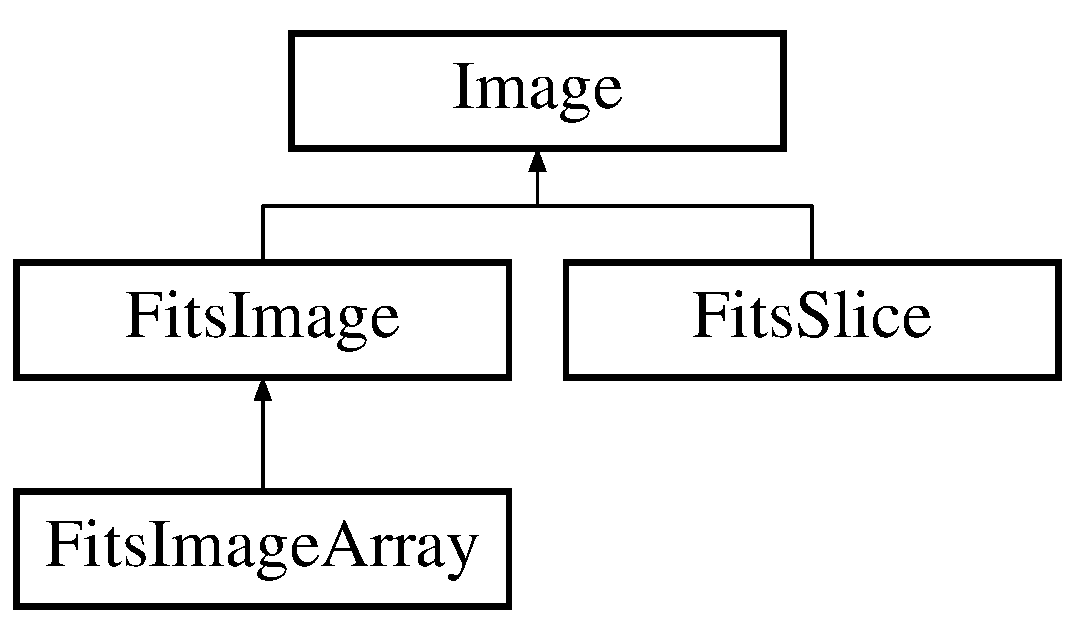
\includegraphics[height=3cm]{class_image}
\end{center}
\end{figure}
\subsubsection*{Public Methods}
\begin{CompactItemize}
\item 
\index{Image@{Image}!Image@{Image}}\index{Image@{Image}!Image@{Image}}
{\bf Image} (const int Nx, const int Ny)\label{class_image_a0}

\begin{CompactList}\small\item\em constructor reserves the needed space to store the pixels.\item\end{CompactList}\item 
\index{Image@{Image}!Image@{Image}}\index{Image@{Image}!Image@{Image}}
{\bf Image} ()\label{class_image_a1}

\begin{CompactList}\small\item\em reserves an empty image.\item\end{CompactList}\item 
\index{Image@{Image}!Image@{Image}}\index{Image@{Image}!Image@{Image}}
{\bf Image} (const Image \&)\label{class_image_a2}

\begin{CompactList}\small\item\em copy constructor.\item\end{CompactList}\item 
\index{~Image@{$\sim$Image}!Image@{Image}}\index{Image@{Image}!~Image@{$\sim$Image}}
virtual {\bf $\sim$Image} ()\label{class_image_a3}

\item 
\index{operator()@{operator()}!Image@{Image}}\index{Image@{Image}!operator()@{operator()}}
Pixel\& {\bf operator()} (const int i, const int j)\label{class_image_a4}

\begin{CompactList}\small\item\em access to the data (RW mode). The first pixel is indexed (0,0).\item\end{CompactList}\item 
\index{operator()@{operator()}!Image@{Image}}\index{Image@{Image}!operator()@{operator()}}
Pixel\& {\bf operator()} (const int i, const int j) const\label{class_image_a5}

\item 
\index{value@{value}!Image@{Image}}\index{Image@{Image}!value@{value}}
Pixel\& {\bf value} (const int i, const int j)\label{class_image_a6}

\item 
\index{MinValue@{MinValue}!Image@{Image}}\index{Image@{Image}!MinValue@{Min\-Value}}
Pixel {\bf Min\-Value} () const\label{class_image_a7}

\begin{CompactList}\small\item\em returns the minimum pixel value.\item\end{CompactList}\item 
\index{MaxValue@{MaxValue}!Image@{Image}}\index{Image@{Image}!MaxValue@{Max\-Value}}
Pixel {\bf Max\-Value} () const\label{class_image_a8}

\begin{CompactList}\small\item\em returns the maximum pixel value.\item\end{CompactList}\item 
\index{MinMaxValue@{MinMaxValue}!Image@{Image}}\index{Image@{Image}!MinMaxValue@{Min\-Max\-Value}}
void {\bf Min\-Max\-Value} (Pixel $\ast$Min, Pixel $\ast$Max) const\label{class_image_a9}

\begin{CompactList}\small\item\em returns both min and max in a single image traversal.\item\end{CompactList}\item 
\index{ClippedMeanSigmaValue@{ClippedMeanSigmaValue}!Image@{Image}}\index{Image@{Image}!ClippedMeanSigmaValue@{Clipped\-Mean\-Sigma\-Value}}
void {\bf Clipped\-Mean\-Sigma\-Value} (double \&Mean, double \&Sigma, Image $\ast$pmask=NULL) const\label{class_image_a10}

\item 
\index{MedianInFrame@{MedianInFrame}!Image@{Image}}\index{Image@{Image}!MedianInFrame@{Median\-In\-Frame}}
Pixel {\bf Median\-In\-Frame} (const {\bf Frame} \&Region, Pixel \&Sigma) const\label{class_image_a11}

\begin{CompactList}\small\item\em computes the median in a region of an image.\item\end{CompactList}\item 
\index{EnforceMinMax@{EnforceMinMax}!Image@{Image}}\index{Image@{Image}!EnforceMinMax@{Enforce\-Min\-Max}}
void {\bf Enforce\-Min\-Max} (Pixel min, Pixel max) const\label{class_image_a12}

\begin{CompactList}\small\item\em enforce the min and max value of the image.\item\end{CompactList}\item 
\index{minx@{minx}!Image@{Image}}\index{Image@{Image}!minx@{minx}}
int {\bf minx} () const\label{class_image_a13}

\item 
\index{maxx@{maxx}!Image@{Image}}\index{Image@{Image}!maxx@{maxx}}
int {\bf maxx} () const\label{class_image_a14}

\item 
\index{miny@{miny}!Image@{Image}}\index{Image@{Image}!miny@{miny}}
int {\bf miny} () const\label{class_image_a15}

\item 
\index{maxy@{maxy}!Image@{Image}}\index{Image@{Image}!maxy@{maxy}}
int {\bf maxy} () const\label{class_image_a16}

\item 
\index{MeanSigmaValue@{MeanSigmaValue}!Image@{Image}}\index{Image@{Image}!MeanSigmaValue@{Mean\-Sigma\-Value}}
void {\bf Mean\-Sigma\-Value} (Pixel $\ast$Mean, Pixel $\ast$Sigma) const\label{class_image_a17}

\begin{CompactList}\small\item\em computes the mean and sigma of an image using 5 loops over ALL image.\item\end{CompactList}\item 
\index{SkyLevel@{SkyLevel}!Image@{Image}}\index{Image@{Image}!SkyLevel@{Sky\-Level}}
void {\bf Sky\-Level} (Pixel $\ast$Mean, Pixel $\ast$Sigma) const\label{class_image_a18}

\begin{CompactList}\small\item\em computes the mean and sigma of an image using the median (from 10000 random pixels) and loop 3 times.\item\end{CompactList}\item 
\index{SkyLevel@{SkyLevel}!Image@{Image}}\index{Image@{Image}!SkyLevel@{Sky\-Level}}
void {\bf Sky\-Level} (const {\bf Frame} \&{\bf Frame}, Pixel $\ast$Mean, Pixel $\ast$Sigma) const\label{class_image_a19}

\item 
\index{Surface@{Surface}!Image@{Image}}\index{Image@{Image}!Surface@{Surface}}
void {\bf Surface} (const int Mesh\-Step, Image \&Result)\label{class_image_a20}

\begin{CompactList}\small\item\em computes a Back\-Image, subtract it, and returns the result in Result (which should have a 0 average).\item\end{CompactList}\item 
\index{dump@{dump}!Image@{Image}}\index{Image@{Image}!dump@{dump}}
void {\bf dump} () const\label{class_image_a21}

\item 
\index{Nx@{Nx}!Image@{Image}}\index{Image@{Image}!Nx@{Nx}}
int {\bf Nx} () const\label{class_image_a22}

\begin{CompactList}\small\item\em returns x size of the image.\item\end{CompactList}\item 
\index{Ny@{Ny}!Image@{Image}}\index{Image@{Image}!Ny@{Ny}}
int {\bf Ny} () const\label{class_image_a23}

\begin{CompactList}\small\item\em returns y size of the image.\item\end{CompactList}\item 
\index{operator=@{operator=}!Image@{Image}}\index{Image@{Image}!operator=@{operator=}}
Image\& {\bf operator=} (const Image \&Right)\label{class_image_a24}

\item 
\index{NPix@{NPix}!Image@{Image}}\index{Image@{Image}!NPix@{NPix}}
int {\bf NPix} () const\label{class_image_a25}

\begin{CompactList}\small\item\em returns number of pixels.\item\end{CompactList}\item 
\index{operator+@{operator+}!Image@{Image}}\index{Image@{Image}!operator+@{operator+}}
Image {\bf operator+} (const Image \&Right) const\label{class_image_a26}

\item 
\index{operator-@{operator-}!Image@{Image}}\index{Image@{Image}!operator-@{operator-}}
Image {\bf operator-} (const Image \&Right) const\label{class_image_a27}

\item 
\index{operator *@{operator $\ast$}!Image@{Image}}\index{Image@{Image}!operator *@{operator $\ast$}}
Image {\bf operator $\ast$} (const Image \&Right) const\label{class_image_a28}

\item 
\index{operator/@{operator/}!Image@{Image}}\index{Image@{Image}!operator/@{operator/}}
Image {\bf operator/} (const Image \&Right) const\label{class_image_a29}

\item 
\index{operator+=@{operator+=}!Image@{Image}}\index{Image@{Image}!operator+=@{operator+=}}
void {\bf operator+=} (const Image \&Right) const\label{class_image_a30}

\item 
\index{operator-=@{operator-=}!Image@{Image}}\index{Image@{Image}!operator-=@{operator-=}}
void {\bf operator-=} (const Image \&Right) const\label{class_image_a31}

\item 
\index{operator *=@{operator $\ast$=}!Image@{Image}}\index{Image@{Image}!operator *=@{operator $\ast$=}}
void {\bf operator $\ast$=} (const Image \&Right) const\label{class_image_a32}

\item 
\index{operator/=@{operator/=}!Image@{Image}}\index{Image@{Image}!operator/=@{operator/=}}
void {\bf operator/=} (const Image \&Right) const\label{class_image_a33}

\item 
\index{operator+@{operator+}!Image@{Image}}\index{Image@{Image}!operator+@{operator+}}
Image {\bf operator+} (const double Right) const\label{class_image_a34}

\item 
\index{operator-@{operator-}!Image@{Image}}\index{Image@{Image}!operator-@{operator-}}
Image {\bf operator-} (const double Right) const\label{class_image_a35}

\item 
\index{operator *@{operator $\ast$}!Image@{Image}}\index{Image@{Image}!operator *@{operator $\ast$}}
Image {\bf operator $\ast$} (const double Right) const\label{class_image_a36}

\item 
\index{operator/@{operator/}!Image@{Image}}\index{Image@{Image}!operator/@{operator/}}
Image {\bf operator/} (const double Right) const\label{class_image_a37}

\item 
\index{operator=@{operator=}!Image@{Image}}\index{Image@{Image}!operator=@{operator=}}
void {\bf operator=} (const double Right)\label{class_image_a38}

\item 
\index{operator+=@{operator+=}!Image@{Image}}\index{Image@{Image}!operator+=@{operator+=}}
void {\bf operator+=} (const double Right)\label{class_image_a39}

\item 
\index{operator-=@{operator-=}!Image@{Image}}\index{Image@{Image}!operator-=@{operator-=}}
void {\bf operator-=} (const double Right)\label{class_image_a40}

\item 
\index{operator *=@{operator $\ast$=}!Image@{Image}}\index{Image@{Image}!operator *=@{operator $\ast$=}}
void {\bf operator $\ast$=} (const double Right)\label{class_image_a41}

\item 
\index{operator/=@{operator/=}!Image@{Image}}\index{Image@{Image}!operator/=@{operator/=}}
void {\bf operator/=} (const double Right)\label{class_image_a42}

\item 
\index{MultiplyBySquare@{MultiplyBySquare}!Image@{Image}}\index{Image@{Image}!MultiplyBySquare@{Multiply\-By\-Square}}
void {\bf Multiply\-By\-Square} (const Image \&Right)\label{class_image_a43}

\begin{CompactList}\small\item\em multiply by the square of the image Right.\item\end{CompactList}\item 
\index{Heavyside@{Heavyside}!Image@{Image}}\index{Image@{Image}!Heavyside@{Heavyside}}
void {\bf Heavyside} ()\label{class_image_a44}

\begin{CompactList}\small\item\em pass the image trough an heaviside function that remove negative pixels.\item\end{CompactList}\item 
\index{Interpolate@{Interpolate}!Image@{Image}}\index{Image@{Image}!Interpolate@{Interpolate}}
Pixel {\bf Interpolate} (const double x, const double y, const int level=3, const bool Is\-Variance\-Map=false) const\label{class_image_a45}

\begin{CompactList}\small\item\em linear interpolation routine. I.Interpolate(0.0,0.0) returns I(0,0).\item\end{CompactList}\item 
\index{GtransfoImage@{GtransfoImage}!Image@{Image}}\index{Image@{Image}!GtransfoImage@{Gtransfo\-Image}}
Image {\bf Gtransfo\-Image} (const {\bf Gtransfo} \&g, int nx, int ny, float Default\-Val, const int interp\-Level=3, const bool Is\-Variance\-Map=false) const\label{class_image_a46}

\begin{CompactList}\small\item\em Image resampling. Can handle Variance maps.\item\end{CompactList}\item 
\index{Subimage@{Subimage}!Image@{Image}}\index{Image@{Image}!Subimage@{Subimage}}
Image {\bf Subimage} (const int x, const int y, const int width, const int height) const\label{class_image_a47}

\begin{CompactList}\small\item\em extract a subimage.\item\end{CompactList}\item 
\index{Subimage@{Subimage}!Image@{Image}}\index{Image@{Image}!Subimage@{Subimage}}
Image {\bf Subimage} (const {\bf Frame} \&frame) const\label{class_image_a48}

\begin{CompactList}\small\item\em extract a subimage.\item\end{CompactList}\item 
\index{SubimageMultiply@{SubimageMultiply}!Image@{Image}}\index{Image@{Image}!SubimageMultiply@{Subimage\-Multiply}}
void {\bf Subimage\-Multiply} (const int x, const int y, const int width, const int height, double factor)\label{class_image_a49}

\begin{CompactList}\small\item\em multiply a subimage by a double.\item\end{CompactList}\item 
\index{SubimageMultiply@{SubimageMultiply}!Image@{Image}}\index{Image@{Image}!SubimageMultiply@{Subimage\-Multiply}}
void {\bf Subimage\-Multiply} (const {\bf Frame} \&frame, double factor)\label{class_image_a50}

\begin{CompactList}\small\item\em multiply a subimage by a double.\item\end{CompactList}\item 
\index{Mask@{Mask}!Image@{Image}}\index{Image@{Image}!Mask@{Mask}}
Image {\bf Mask} (const int x\_\-Beg, const int y\_\-Beg, const int x\_\-End, const int y\_\-End) const\label{class_image_a51}

\begin{CompactList}\small\item\em keep the pixels inside the mask and put the other at 0.0.\item\end{CompactList}\item 
\index{Masking@{Masking}!Image@{Image}}\index{Image@{Image}!Masking@{Masking}}
void {\bf Masking} (const {\bf Frame} \&frame, const Pixel \&Mask\-Value=1)\label{class_image_a52}

\begin{CompactList}\small\item\em put the pixels outside mask to Mask\-Value.\item\end{CompactList}\item 
\index{DiskMaskIt@{DiskMaskIt}!Image@{Image}}\index{Image@{Image}!DiskMaskIt@{Disk\-Mask\-It}}
void {\bf Disk\-Mask\-It} (const double \&xc, const double \&yc, const double \&radius)\label{class_image_a53}

\begin{CompactList}\small\item\em put the pixels outside a disk to 1.\item\end{CompactList}\item 
\index{Truncate@{Truncate}!Image@{Image}}\index{Image@{Image}!Truncate@{Truncate}}
void {\bf Truncate} (const double \&xc, const double \&yc, const double \&radius)\label{class_image_a54}

\begin{CompactList}\small\item\em put the pixels outside a disk to 0.\item\end{CompactList}\item 
\index{Masking@{Masking}!Image@{Image}}\index{Image@{Image}!Masking@{Masking}}
void {\bf Masking} (const int x\_\-Beg, const int y\_\-Beg, const int x\_\-End, const int y\_\-End, const Pixel \&Mask\-Value=1)\label{class_image_a55}

\item 
\index{Simplify@{Simplify}!Image@{Image}}\index{Image@{Image}!Simplify@{Simplify}}
void {\bf Simplify} (double threshold, int above\_\-val=1, int under\_\-val=0)\label{class_image_a56}

\begin{CompactList}\small\item\em put pixels above threshold to 1 and to 0 otherwise.\item\end{CompactList}\item 
\index{RemoveLonePix@{RemoveLonePix}!Image@{Image}}\index{Image@{Image}!RemoveLonePix@{Remove\-Lone\-Pix}}
void {\bf Remove\-Lone\-Pix} (Image \&result, int d=1)\label{class_image_a57}

\begin{CompactList}\small\item\em remove lone bad pixels ie with no bad pixels in a square of 2d+1 x 2d+1.\item\end{CompactList}\item 
\index{SumPixels@{SumPixels}!Image@{Image}}\index{Image@{Image}!SumPixels@{Sum\-Pixels}}
double {\bf Sum\-Pixels} ()\label{class_image_a58}

\begin{CompactList}\small\item\em sum pixels values.\item\end{CompactList}\item 
\index{SumSquaredPixels@{SumSquaredPixels}!Image@{Image}}\index{Image@{Image}!SumSquaredPixels@{Sum\-Squared\-Pixels}}
double {\bf Sum\-Squared\-Pixels} () const\label{class_image_a59}

\begin{CompactList}\small\item\em sum of the squared pixel values.\item\end{CompactList}\item 
\index{MedianFilter@{MedianFilter}!Image@{Image}}\index{Image@{Image}!MedianFilter@{Median\-Filter}}
void {\bf Median\-Filter} (const int Half\-Width)\label{class_image_a60}

\item 
\index{begin@{begin}!Image@{Image}}\index{Image@{Image}!begin@{begin}}
Pixel$\ast$ {\bf begin} ()\label{class_image_a61}

\begin{CompactList}\small\item\em returns the pointer to the first pixel.\item\end{CompactList}\item 
\index{begin@{begin}!Image@{Image}}\index{Image@{Image}!begin@{begin}}
Pixel$\ast$ {\bf begin} () const\label{class_image_a62}

\item 
\index{end@{end}!Image@{Image}}\index{Image@{Image}!end@{end}}
Pixel$\ast$ {\bf end} ()\label{class_image_a63}

\begin{CompactList}\small\item\em returns the pointer to the next to last pixel, as usual for containers.\item\end{CompactList}\item 
\index{end@{end}!Image@{Image}}\index{Image@{Image}!end@{end}}
Pixel$\ast$ {\bf end} () const\label{class_image_a64}

\item 
\index{SameSize@{SameSize}!Image@{Image}}\index{Image@{Image}!SameSize@{Same\-Size}}
bool {\bf Same\-Size} (const Image \&Other) const\label{class_image_a65}

\item 
int {\bf Laplacian\-Filter} (const double \&Sigma, const double \&Mean, const double \&seeing, Image \&Cosmic\-Image)
\begin{CompactList}\small\item\em Builds a cosmic map.\item\end{CompactList}\item 
\index{Cosmics@{Cosmics}!Image@{Image}}\index{Image@{Image}!Cosmics@{Cosmics}}
void {\bf Cosmics} (const double \&Sigma, const double \&Mean, const double \&seeing, Image \&Cosmic\-Image)\label{class_image_a67}

\begin{CompactList}\small\item\em returns the final cosmic map(after iterations).\item\end{CompactList}\item 
\index{ApplyFun@{ApplyFun}!Image@{Image}}\index{Image@{Image}!ApplyFun@{Apply\-Fun}}
void {\bf Apply\-Fun} (double(\&F)(double))\label{class_image_a68}

\end{CompactItemize}
\subsubsection*{Protected Methods}
\begin{CompactItemize}
\item 
\index{allocate@{allocate}!Image@{Image}}\index{Image@{Image}!allocate@{allocate}}
void {\bf allocate} (int Nx, int Ny, int Init=1)\label{class_image_b0}

\item 
\index{get_elem_ref@{get\_\-elem\_\-ref}!Image@{Image}}\index{Image@{Image}!get_elem_ref@{get\_\-elem\_\-ref}}
Pixel$\ast$ {\bf get\_\-elem\_\-ref} (int i, int j)\label{class_image_b1}

\end{CompactItemize}
\subsubsection*{Protected Attributes}
\begin{CompactItemize}
\item 
\index{data@{data}!Image@{Image}}\index{Image@{Image}!data@{data}}
Pixel$\ast$ {\bf data}\label{class_image_n0}

\item 
\index{nx@{nx}!Image@{Image}}\index{Image@{Image}!nx@{nx}}
int {\bf nx}\label{class_image_n1}

\item 
\index{ny@{ny}!Image@{Image}}\index{Image@{Image}!ny@{ny}}
int {\bf ny}\label{class_image_n2}

\end{CompactItemize}
\subsubsection*{Friends}
\begin{CompactItemize}
\item 
class {\bf Fits\-Image\-Array}
\item 
class {\bf operator+}
\item 
class {\bf operator-}
\item 
class {\bf operator $\ast$}
\item 
class {\bf operator/}
\item 
class {\bf image\_\-copy}
\end{CompactItemize}


\subsubsection{Detailed Description}
Class for the basic manipulation of images.

The internal representation uses (32 bits) float numbers, designated later as the Pixel type. 



\subsubsection{Member Function Documentation}
\index{Image@{Image}!LaplacianFilter@{LaplacianFilter}}
\index{LaplacianFilter@{LaplacianFilter}!Image@{Image}}
\paragraph{\setlength{\rightskip}{0pt plus 5cm}int Image::Laplacian\-Filter (const double \& {\em Sigma}, const double \& {\em Mean}, const double \& {\em seeing}, Image \& {\em Cosmic\-Image})}\hfill\label{class_image_a66}


Builds a cosmic map.

Cuts (based on the article -$>$ astro-ph/0108003):  -cut\_\-lap : the laplacian operator increases the noise by a factor of  \char`\"{}sqrt(1.25)\char`\"{}

-cut\_\-f : 2$\ast$sigma(med), where sigma(med) is the variance of the sky's median calculated in a box (3$\ast$3), here.  (sigma(med) = sigma(sky)$\ast$1.22/sqrt(n); n = size of the box)

-cut\_\-lf : calculated from the article. Factor 2.35 -$>$ to have the seeing in arc sec 

The documentation for this class was generated from the following files:\begin{CompactItemize}
\item 
{\bf image.h}\item 
image.cc\end{CompactItemize}

\subsection{Image\-Back  Class Reference}
\label{class_imageback}\index{ImageBack@{Image\-Back}}
{\bf Image} {\rm (p.\,\pageref{class_image})} Back class to compute an image of the background. 


{\tt \#include $<$imageback.h$>$}

\subsubsection*{Public Methods}
\begin{CompactItemize}
\item 
{\bf Image\-Back} ({\bf Image} const \&Source\-Image, int Mesh\-Step, const {\bf Image} $\ast$Weight=NULL)
\item 
{\bf Image\-Back} ({\bf Image} const \&Source\-Image, int Mesh\-Step\-X, int Mesh\-Step\-Y, const {\bf Image} $\ast$Weight=NULL)
\item 
\index{Nx@{Nx}!ImageBack@{Image\-Back}}\index{ImageBack@{ImageBack}!Nx@{Nx}}
int {\bf Nx} () const\label{class_imageback_a2}

\item 
\index{Ny@{Ny}!ImageBack@{Image\-Back}}\index{ImageBack@{ImageBack}!Ny@{Ny}}
int {\bf Ny} () const\label{class_imageback_a3}

\item 
Pixel {\bf Value} (const int i, const int j) const
\item 
Pixel {\bf Rms} (const int i, const int j) const
\item 
{\bf Image}$\ast$ {\bf Background\-Image} ()
\item 
\index{BackValue@{BackValue}!ImageBack@{Image\-Back}}\index{ImageBack@{ImageBack}!BackValue@{Back\-Value}}
const {\bf Image}\& {\bf Back\-Value} () const\label{class_imageback_a7}

\item 
\index{BackRms@{BackRms}!ImageBack@{Image\-Back}}\index{ImageBack@{ImageBack}!BackRms@{Back\-Rms}}
const {\bf Image}\& {\bf Back\-Rms} () const\label{class_imageback_a8}

\item 
\index{Write@{Write}!ImageBack@{Image\-Back}}\index{ImageBack@{ImageBack}!Write@{Write}}
int {\bf Write} (string File\-Name)\label{class_imageback_a9}

\item 
\index{ImageBack@{ImageBack}!ImageBack@{Image\-Back}}\index{ImageBack@{ImageBack}!ImageBack@{Image\-Back}}
{\bf Image\-Back} (char $\ast$File\-Name, const {\bf Image} \&Source)\label{class_imageback_a10}

\end{CompactItemize}


\subsubsection{Detailed Description}
{\bf Image} {\rm (p.\,\pageref{class_image})} Back class to compute an image of the background.



\subsubsection{Constructor \& Destructor Documentation}
\index{ImageBack@{Image\-Back}!ImageBack@{ImageBack}}
\index{ImageBack@{ImageBack}!ImageBack@{Image\-Back}}
\paragraph{\setlength{\rightskip}{0pt plus 5cm}Image\-Back::Image\-Back ({\bf Image} const \& {\em Source\-Image}, int {\em Mesh\-Step}, const {\bf Image} $\ast$ {\em Weight} = NULL)}\hfill\label{class_imageback_a0}


The constructor for a square Mesh (Mesh\-Step\-X=Mesh\-Step\-Y). \index{ImageBack@{Image\-Back}!ImageBack@{ImageBack}}
\index{ImageBack@{ImageBack}!ImageBack@{Image\-Back}}
\paragraph{\setlength{\rightskip}{0pt plus 5cm}Image\-Back::Image\-Back ({\bf Image} const \& {\em Source\-Image}, int {\em Mesh\-Step\-X}, int {\em Mesh\-Step\-Y}, const {\bf Image} $\ast$ {\em Weight} = NULL)}\hfill\label{class_imageback_a1}


The constructor for a rectangular Mesh (Mesh\-Step\-X!=Mesh\-Step\-Y). 

\subsubsection{Member Function Documentation}
\index{ImageBack@{Image\-Back}!BackgroundImage@{BackgroundImage}}
\index{BackgroundImage@{BackgroundImage}!ImageBack@{Image\-Back}}
\paragraph{\setlength{\rightskip}{0pt plus 5cm}{\bf Image} $\ast$ Image\-Back::Background\-Image ()}\hfill\label{class_imageback_a6}


returns the average background image in the coordinates of the original image. \index{ImageBack@{Image\-Back}!Rms@{Rms}}
\index{Rms@{Rms}!ImageBack@{Image\-Back}}
\paragraph{\setlength{\rightskip}{0pt plus 5cm}Pixel Image\-Back::Rms (const int {\em i}, const int {\em j}) const}\hfill\label{class_imageback_a5}


same for Rms. \index{ImageBack@{Image\-Back}!Value@{Value}}
\index{Value@{Value}!ImageBack@{Image\-Back}}
\paragraph{\setlength{\rightskip}{0pt plus 5cm}Pixel Image\-Back::Value (const int {\em i}, const int {\em j}) const}\hfill\label{class_imageback_a4}


returns the average background for pixel (i,j) in the coordinates of the original image. 

The documentation for this class was generated from the following file:\begin{CompactItemize}
\item 
{\bf imageback.h}\end{CompactItemize}

\subsection{Image\-Gtransfo  Class Reference}
\label{class_imagegtransfo}\index{ImageGtransfo@{Image\-Gtransfo}}
{\tt \#include $<$transformedimage.h$>$}

Inheritance diagram for Image\-Gtransfo::\begin{figure}[H]
\begin{center}
\leavevmode
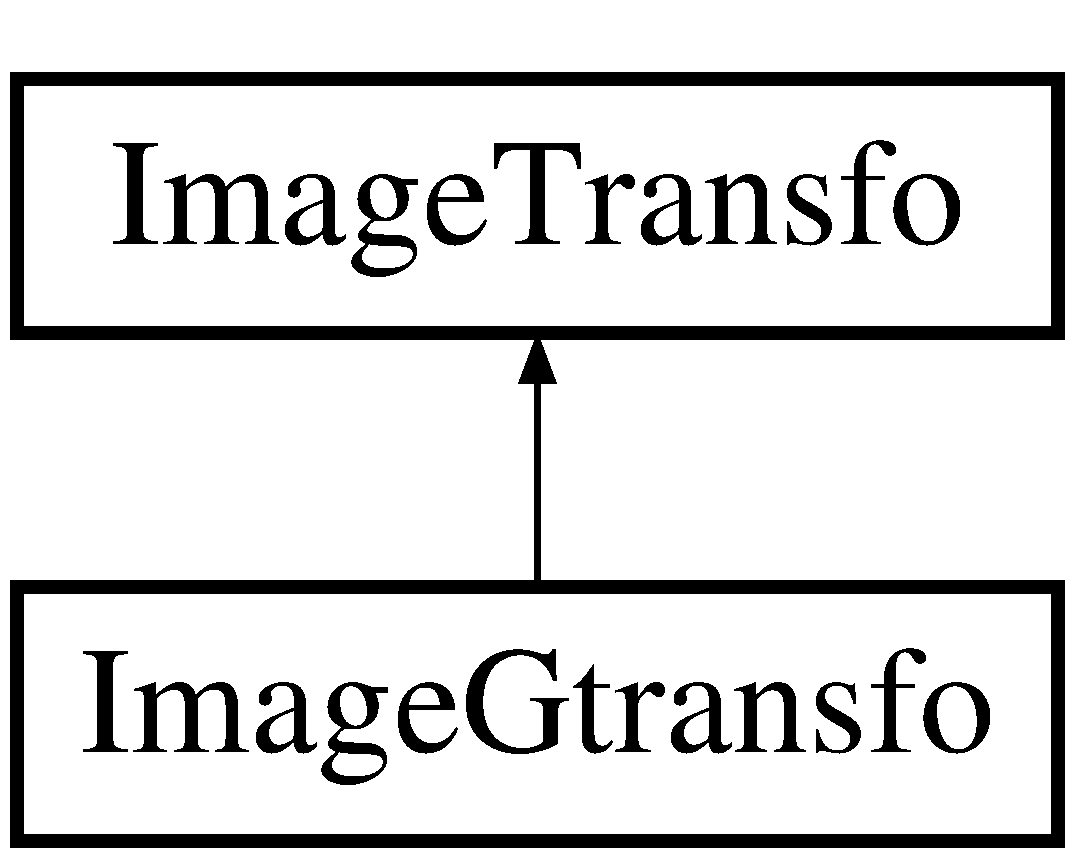
\includegraphics[height=2cm]{class_imagegtransfo}
\end{center}
\end{figure}
\subsubsection*{Public Methods}
\begin{CompactItemize}
\item 
\index{ImageGtransfo@{ImageGtransfo}!ImageGtransfo@{Image\-Gtransfo}}\index{ImageGtransfo@{ImageGtransfo}!ImageGtransfo@{Image\-Gtransfo}}
{\bf Image\-Gtransfo} (const {\bf Gtransfo} $\ast$Transfo\-From\-Ref, const {\bf Gtransfo} $\ast$Transfo\-To\-Ref, const {\bf Frame} \&Output\-Image\-Size, const string \&Geom\-Ref\-Name)\label{class_imagegtransfo_a0}

\item 
\index{ImageGtransfo@{ImageGtransfo}!ImageGtransfo@{Image\-Gtransfo}}\index{ImageGtransfo@{ImageGtransfo}!ImageGtransfo@{Image\-Gtransfo}}
{\bf Image\-Gtransfo} (const {\bf Reduced\-Image} \&Ref, const {\bf Reduced\-Image} \&To\-Align)\label{class_imagegtransfo_a1}

\begin{CompactList}\small\item\em the output image size is the one of the Ref. Finds the transfo(s).\item\end{CompactList}\item 
\index{ImageGtransfo@{ImageGtransfo}!ImageGtransfo@{Image\-Gtransfo}}\index{ImageGtransfo@{ImageGtransfo}!ImageGtransfo@{Image\-Gtransfo}}
{\bf Image\-Gtransfo} ()\label{class_imagegtransfo_a2}

\item 
\index{TransfoFromRef@{TransfoFromRef}!ImageGtransfo@{Image\-Gtransfo}}\index{ImageGtransfo@{ImageGtransfo}!TransfoFromRef@{Transfo\-From\-Ref}}
{\bf Gtransfo}$\ast$ {\bf Transfo\-From\-Ref} () const\label{class_imagegtransfo_a3}

\item 
\index{TransfoToRef@{TransfoToRef}!ImageGtransfo@{Image\-Gtransfo}}\index{ImageGtransfo@{ImageGtransfo}!TransfoToRef@{Transfo\-To\-Ref}}
{\bf Gtransfo}$\ast$ {\bf Transfo\-To\-Ref} () const\label{class_imagegtransfo_a4}

\item 
\index{FromRef@{FromRef}!ImageGtransfo@{Image\-Gtransfo}}\index{ImageGtransfo@{ImageGtransfo}!FromRef@{From\-Ref}}
const {\bf Gtransfo}$\ast$ {\bf From\-Ref} () const\label{class_imagegtransfo_a5}

\item 
\index{GeomRefName@{GeomRefName}!ImageGtransfo@{Image\-Gtransfo}}\index{ImageGtransfo@{ImageGtransfo}!GeomRefName@{Geom\-Ref\-Name}}
string {\bf Geom\-Ref\-Name} () const\label{class_imagegtransfo_a6}

\item 
\index{dump@{dump}!ImageGtransfo@{Image\-Gtransfo}}\index{ImageGtransfo@{ImageGtransfo}!dump@{dump}}
virtual void {\bf dump} (ostream \&s=cout)\label{class_imagegtransfo_a7}

\item 
\index{TransformImage@{TransformImage}!ImageGtransfo@{Image\-Gtransfo}}\index{ImageGtransfo@{ImageGtransfo}!TransformImage@{Transform\-Image}}
void {\bf Transform\-Image} (const {\bf Fits\-Image} \&Source, {\bf Fits\-Image} \&Transformed, const {\bf Reduced\-Image} $\ast$Source, {\bf Reduced\-Image} $\ast$Result, double Default\-Val=0) const\label{class_imagegtransfo_a8}

\begin{CompactList}\small\item\em the one that transforms the image and update header.\item\end{CompactList}\item 
\index{TransformWeightImage@{TransformWeightImage}!ImageGtransfo@{Image\-Gtransfo}}\index{ImageGtransfo@{ImageGtransfo}!TransformWeightImage@{Transform\-Weight\-Image}}
void {\bf Transform\-Weight\-Image} (const {\bf Fits\-Image} \&Source, {\bf Fits\-Image} \&Transformed) const\label{class_imagegtransfo_a9}

\begin{CompactList}\small\item\em Transforms a weight image.\item\end{CompactList}\item 
\index{TransformBoolImage@{TransformBoolImage}!ImageGtransfo@{Image\-Gtransfo}}\index{ImageGtransfo@{ImageGtransfo}!TransformBoolImage@{Transform\-Bool\-Image}}
void {\bf Transform\-Bool\-Image} (const {\bf Fits\-Image} \&Source, {\bf Fits\-Image} \&Transformed) const\label{class_imagegtransfo_a10}

\begin{CompactList}\small\item\em transforms a bool {\bf Image} {\rm (p.\,\pageref{class_image})}.\item\end{CompactList}\item 
\index{TransformCatalog@{TransformCatalog}!ImageGtransfo@{Image\-Gtransfo}}\index{ImageGtransfo@{ImageGtransfo}!TransformCatalog@{Transform\-Catalog}}
void {\bf Transform\-Catalog} (const {\bf SEStar\-List} \&Catalog, {\bf SEStar\-List} \&Transformed) const\label{class_imagegtransfo_a11}

\item 
\index{IsValid@{IsValid}!ImageGtransfo@{Image\-Gtransfo}}\index{ImageGtransfo@{ImageGtransfo}!IsValid@{Is\-Valid}}
bool {\bf Is\-Valid} () const\label{class_imagegtransfo_a12}

\item 
\index{ScaleFactor@{ScaleFactor}!ImageGtransfo@{Image\-Gtransfo}}\index{ImageGtransfo@{ImageGtransfo}!ScaleFactor@{Scale\-Factor}}
double {\bf Scale\-Factor} () const\label{class_imagegtransfo_a13}

\item 
\index{Clone@{Clone}!ImageGtransfo@{Image\-Gtransfo}}\index{ImageGtransfo@{ImageGtransfo}!Clone@{Clone}}
Image\-Transfo$\ast$ {\bf Clone} () const\label{class_imagegtransfo_a14}

\item 
\index{~ImageGtransfo@{$\sim$ImageGtransfo}!ImageGtransfo@{Image\-Gtransfo}}\index{ImageGtransfo@{ImageGtransfo}!~ImageGtransfo@{$\sim$Image\-Gtransfo}}
{\bf $\sim$Image\-Gtransfo} ()\label{class_imagegtransfo_a15}

\end{CompactItemize}


\subsubsection{Detailed Description}
geometric transfo of a reduced image. 



The documentation for this class was generated from the following file:\begin{CompactItemize}
\item 
{\bf transformedimage.h}\end{CompactItemize}

\subsection{Image\-Subtraction  Class Reference}
\label{class_imagesubtraction}\index{ImageSubtraction@{Image\-Subtraction}}
For subtracting images using the Alard kernel fit technique. A basic assumption: Ref and New are already geometrically aligned. 


{\tt \#include $<$imagesubtraction.h$>$}

Inheritance diagram for Image\-Subtraction::\begin{figure}[H]
\begin{center}
\leavevmode
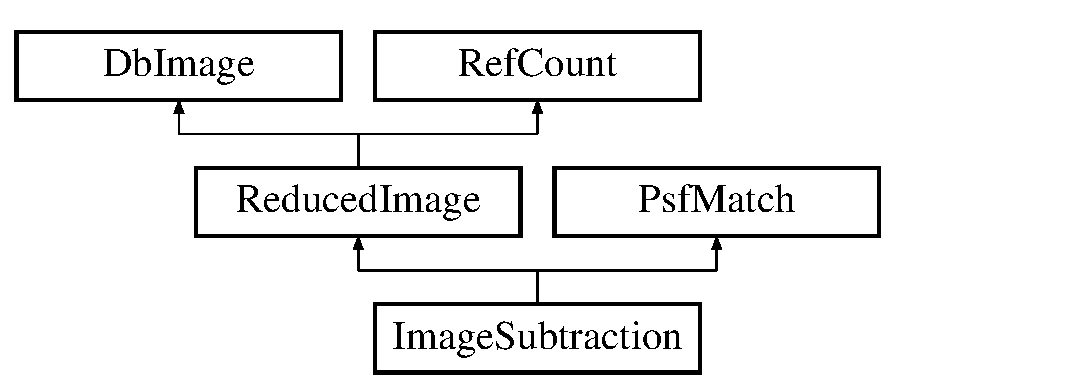
\includegraphics[height=3cm]{class_imagesubtraction}
\end{center}
\end{figure}
\subsubsection*{Public Methods}
\begin{CompactItemize}
\item 
\index{ImageSubtraction@{ImageSubtraction}!ImageSubtraction@{Image\-Subtraction}}\index{ImageSubtraction@{ImageSubtraction}!ImageSubtraction@{Image\-Subtraction}}
{\bf Image\-Subtraction} (const string \&Name, const {\bf Reduced\-Image} \&Ref\-Image, const {\bf Reduced\-Image} \&New\-Image)\label{class_imagesubtraction_a0}

\begin{CompactList}\small\item\em the constructor takes a copy of both {\bf Reduced\-Image} {\rm (p.\,\pageref{class_reducedimage})}.\item\end{CompactList}\item 
\index{ImageSubtraction@{ImageSubtraction}!ImageSubtraction@{Image\-Subtraction}}\index{ImageSubtraction@{ImageSubtraction}!ImageSubtraction@{Image\-Subtraction}}
{\bf Image\-Subtraction} (const string \&Name, const {\bf Reduced\-Image} \&Ref\-Image, const {\bf Reduced\-Image} \&New\-Image, const {\bf Psf\-Match} $\ast$AMatch)\label{class_imagesubtraction_a1}

\begin{CompactList}\small\item\em as above but uses kernel found by other means. used for fakes SN.\item\end{CompactList}\item 
\index{ImageSubtraction@{ImageSubtraction}!ImageSubtraction@{Image\-Subtraction}}\index{ImageSubtraction@{ImageSubtraction}!ImageSubtraction@{Image\-Subtraction}}
{\bf Image\-Subtraction} (const string \&Name)\label{class_imagesubtraction_a2}

\item 
\index{MakeFits@{MakeFits}!ImageSubtraction@{Image\-Subtraction}}\index{ImageSubtraction@{ImageSubtraction}!MakeFits@{Make\-Fits}}
bool {\bf Make\-Fits} ()\label{class_imagesubtraction_a3}

\begin{CompactList}\small\item\em Carry out the kernel fit, convolve, and outputs the subtraction image.\item\end{CompactList}\item 
\index{MakeWeight@{MakeWeight}!ImageSubtraction@{Image\-Subtraction}}\index{ImageSubtraction@{ImageSubtraction}!MakeWeight@{Make\-Weight}}
bool {\bf Make\-Weight} ()\label{class_imagesubtraction_a4}

\item 
\index{MakeCatalog@{MakeCatalog}!ImageSubtraction@{Image\-Subtraction}}\index{ImageSubtraction@{ImageSubtraction}!MakeCatalog@{Make\-Catalog}}
bool {\bf Make\-Catalog} ()\label{class_imagesubtraction_a5}

\begin{CompactList}\small\item\em carry out the detection. Default is matched filter plus apreture photometry.\item\end{CompactList}\item 
\index{MakeDead@{MakeDead}!ImageSubtraction@{Image\-Subtraction}}\index{ImageSubtraction@{ImageSubtraction}!MakeDead@{Make\-Dead}}
bool {\bf Make\-Dead} ()\label{class_imagesubtraction_a6}

\begin{CompactList}\small\item\em produce dead image.\item\end{CompactList}\item 
\index{MakeSatur@{MakeSatur}!ImageSubtraction@{Image\-Subtraction}}\index{ImageSubtraction@{ImageSubtraction}!MakeSatur@{Make\-Satur}}
bool {\bf Make\-Satur} ()\label{class_imagesubtraction_a7}

\begin{CompactList}\small\item\em Satur frame is the OR of Ref and New satur frames.\item\end{CompactList}\item 
\index{MaskSatur@{MaskSatur}!ImageSubtraction@{Image\-Subtraction}}\index{ImageSubtraction@{ImageSubtraction}!MaskSatur@{Mask\-Satur}}
bool {\bf Mask\-Satur} ()\label{class_imagesubtraction_a8}

\begin{CompactList}\small\item\em Mask the saturation on the subtraction.\item\end{CompactList}\item 
\index{RunDetection@{RunDetection}!ImageSubtraction@{Image\-Subtraction}}\index{ImageSubtraction@{ImageSubtraction}!RunDetection@{Run\-Detection}}
bool {\bf Run\-Detection} (Detection\-List \&Detections, const Base\-Star\-List $\ast$Positions=NULL)\label{class_imagesubtraction_a9}

\item 
\index{CandName@{CandName}!ImageSubtraction@{Image\-Subtraction}}\index{ImageSubtraction@{ImageSubtraction}!CandName@{Cand\-Name}}
string {\bf Cand\-Name} () const\label{class_imagesubtraction_a10}

\begin{CompactList}\small\item\em Name of the candidates list.\item\end{CompactList}\item 
\index{AllCandName@{AllCandName}!ImageSubtraction@{Image\-Subtraction}}\index{ImageSubtraction@{ImageSubtraction}!AllCandName@{All\-Cand\-Name}}
string {\bf All\-Cand\-Name} () const\label{class_imagesubtraction_a11}

\item 
\index{CandCutName@{CandCutName}!ImageSubtraction@{Image\-Subtraction}}\index{ImageSubtraction@{ImageSubtraction}!CandCutName@{Cand\-Cut\-Name}}
string {\bf Cand\-Cut\-Name} () const\label{class_imagesubtraction_a12}

\item 
\index{CandScanName@{CandScanName}!ImageSubtraction@{Image\-Subtraction}}\index{ImageSubtraction@{ImageSubtraction}!CandScanName@{Cand\-Scan\-Name}}
string {\bf Cand\-Scan\-Name} () const\label{class_imagesubtraction_a13}

\item 
\index{CandCutScanName@{CandCutScanName}!ImageSubtraction@{Image\-Subtraction}}\index{ImageSubtraction@{ImageSubtraction}!CandCutScanName@{Cand\-Cut\-Scan\-Name}}
string {\bf Cand\-Cut\-Scan\-Name} () const\label{class_imagesubtraction_a14}

\item 
\index{DetectionsName@{DetectionsName}!ImageSubtraction@{Image\-Subtraction}}\index{ImageSubtraction@{ImageSubtraction}!DetectionsName@{Detections\-Name}}
string {\bf Detections\-Name} () const\label{class_imagesubtraction_a15}

\item 
\index{MatchedCatName@{MatchedCatName}!ImageSubtraction@{Image\-Subtraction}}\index{ImageSubtraction@{ImageSubtraction}!MatchedCatName@{Matched\-Cat\-Name}}
string {\bf Matched\-Cat\-Name} () const\label{class_imagesubtraction_a16}

\item 
\index{Clone@{Clone}!ImageSubtraction@{Image\-Subtraction}}\index{ImageSubtraction@{ImageSubtraction}!Clone@{Clone}}
{\bf Reduced\-Image}$\ast$ {\bf Clone} () const\label{class_imagesubtraction_a17}

\item 
\index{AllCandidateCatalogName@{AllCandidateCatalogName}!ImageSubtraction@{Image\-Subtraction}}\index{ImageSubtraction@{ImageSubtraction}!AllCandidateCatalogName@{All\-Candidate\-Catalog\-Name}}
string {\bf All\-Candidate\-Catalog\-Name} () const\label{class_imagesubtraction_a18}

\item 
\index{~ImageSubtraction@{$\sim$ImageSubtraction}!ImageSubtraction@{Image\-Subtraction}}\index{ImageSubtraction@{ImageSubtraction}!~ImageSubtraction@{$\sim$Image\-Subtraction}}
{\bf $\sim$Image\-Subtraction} ()\label{class_imagesubtraction_a19}

\item 
\index{ClassDef@{ClassDef}!ImageSubtraction@{Image\-Subtraction}}\index{ImageSubtraction@{ImageSubtraction}!ClassDef@{Class\-Def}}
{\bf Class\-Def} (Image\-Subtraction, 1)\label{class_imagesubtraction_a20}

\end{CompactItemize}


\subsubsection{Detailed Description}
For subtracting images using the Alard kernel fit technique. A basic assumption: Ref and New are already geometrically aligned.



The documentation for this class was generated from the following file:\begin{CompactItemize}
\item 
{\bf imagesubtraction.h}\end{CompactItemize}

\subsection{Image\-Sum  Class Reference}
\label{class_imagesum}\index{ImageSum@{Image\-Sum}}
A class that handles coadding. Shift and coadd is handled by. 


{\tt \#include $<$imagesum.h$>$}

Inheritance diagram for Image\-Sum::\begin{figure}[H]
\begin{center}
\leavevmode
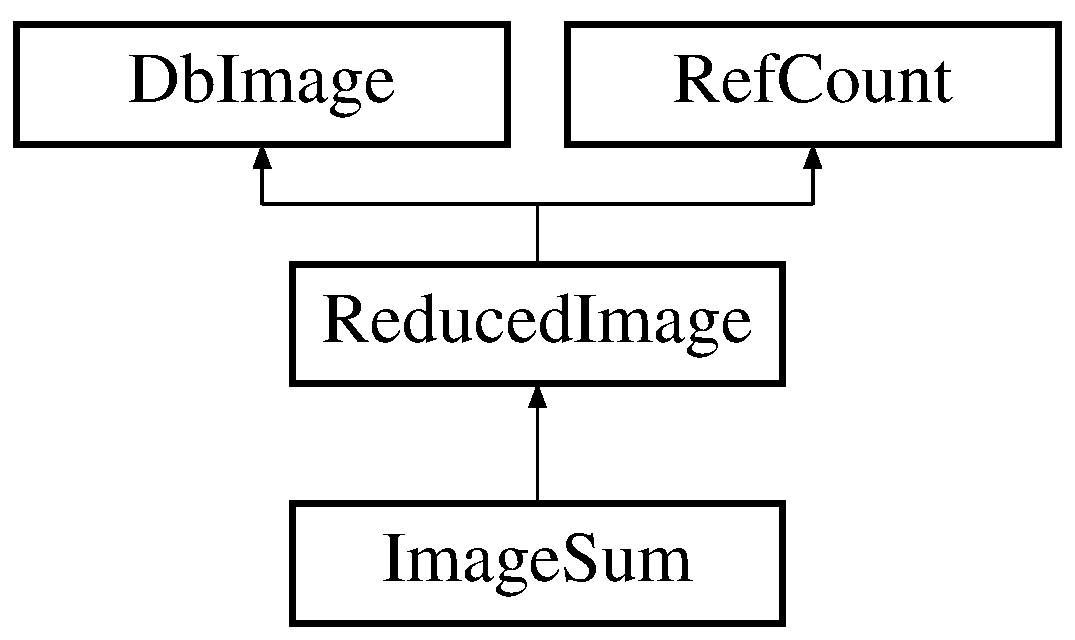
\includegraphics[height=3cm]{class_imagesum}
\end{center}
\end{figure}
\subsubsection*{Public Types}
\begin{CompactItemize}
\item 
\index{ComponentIterator@{ComponentIterator}!ImageSum@{Image\-Sum}}\index{ImageSum@{ImageSum}!ComponentIterator@{Component\-Iterator}}
typedef vector$<${\bf Component}$>$::iterator {\bf Component\-Iterator}\label{class_imagesum_s0}

\item 
\index{ComponentCIterator@{ComponentCIterator}!ImageSum@{Image\-Sum}}\index{ImageSum@{ImageSum}!ComponentCIterator@{Component\-CIterator}}
typedef vector$<${\bf Component}$>$::const\_\-iterator {\bf Component\-CIterator}\label{class_imagesum_s1}

\end{CompactItemize}
\subsubsection*{Public Methods}
\begin{CompactItemize}
\item 
\index{ImageSum@{ImageSum}!ImageSum@{Image\-Sum}}\index{ImageSum@{ImageSum}!ImageSum@{Image\-Sum}}
{\bf Image\-Sum} (const string \&Name, Reduced\-Image\-List \&Images, const {\bf Reduced\-Image} $\ast$Photom\-Reference=NULL, const Weighting\-Method AWMethod=WUn\-Set, const Stacking\-Method ASMethod=SUn\-Set)\label{class_imagesum_a0}

\item 
\index{ImageSum@{ImageSum}!ImageSum@{Image\-Sum}}\index{ImageSum@{ImageSum}!ImageSum@{Image\-Sum}}
{\bf Image\-Sum} (const string \&Name)\label{class_imagesum_a1}

\item 
\index{ImageSum@{ImageSum}!ImageSum@{Image\-Sum}}\index{ImageSum@{ImageSum}!ImageSum@{Image\-Sum}}
{\bf Image\-Sum} ()\label{class_imagesum_a2}

\item 
\index{Components@{Components}!ImageSum@{Image\-Sum}}\index{ImageSum@{ImageSum}!Components@{Components}}
Reduced\-Image\-List {\bf Components} () const\label{class_imagesum_a3}

\item 
\index{MakeFits@{MakeFits}!ImageSum@{Image\-Sum}}\index{ImageSum@{ImageSum}!MakeFits@{Make\-Fits}}
bool {\bf Make\-Fits} ()\label{class_imagesum_a4}

\begin{CompactList}\small\item\em produce fits image.\item\end{CompactList}\item 
\index{MakeCatalog@{MakeCatalog}!ImageSum@{Image\-Sum}}\index{ImageSum@{ImageSum}!MakeCatalog@{Make\-Catalog}}
bool {\bf Make\-Catalog} ()\label{class_imagesum_a5}

\begin{CompactList}\small\item\em Produce the Saturated stars pixels mask, subtract the image background, detect with the SExtractor computed sigma. search the cosmics, and update catalog and weight for cosmics. No free coffee.\item\end{CompactList}\item 
\index{MakeDead@{MakeDead}!ImageSum@{Image\-Sum}}\index{ImageSum@{ImageSum}!MakeDead@{Make\-Dead}}
bool {\bf Make\-Dead} ()\label{class_imagesum_a6}

\begin{CompactList}\small\item\em produce dead image.\item\end{CompactList}\item 
\index{MakeSatur@{MakeSatur}!ImageSum@{Image\-Sum}}\index{ImageSum@{ImageSum}!MakeSatur@{Make\-Satur}}
bool {\bf Make\-Satur} ()\label{class_imagesum_a7}

\begin{CompactList}\small\item\em produce satur image.\item\end{CompactList}\item 
\index{MakeWeight@{MakeWeight}!ImageSum@{Image\-Sum}}\index{ImageSum@{ImageSum}!MakeWeight@{Make\-Weight}}
bool {\bf Make\-Weight} ()\label{class_imagesum_a8}

\item 
\index{Create@{Create}!ImageSum@{Image\-Sum}}\index{ImageSum@{ImageSum}!Create@{Create}}
bool {\bf Create} (const string \&Where)\label{class_imagesum_a9}

\begin{CompactList}\small\item\em To create the directories where the fits images, catalogues will be put: ex: $\sim$/Fake\-Db/test: {\bf Db\-Image} {\rm (p.\,\pageref{class_dbimage})} dbim(\char`\"{}test\char`\"{}); dbim.Create(\char`\"{}$\sim$/Fake\-Db/\char`\"{});.\item\end{CompactList}\item 
\index{Clone@{Clone}!ImageSum@{Image\-Sum}}\index{ImageSum@{ImageSum}!Clone@{Clone}}
{\bf Reduced\-Image}$\ast$ {\bf Clone} () const\label{class_imagesum_a10}

\item 
\index{dump@{dump}!ImageSum@{Image\-Sum}}\index{ImageSum@{ImageSum}!dump@{dump}}
void {\bf dump} (ostream \&s=cout) const\label{class_imagesum_a11}

\begin{CompactList}\small\item\em dumps basic info.\item\end{CompactList}\item 
\index{ClassDef@{ClassDef}!ImageSum@{Image\-Sum}}\index{ImageSum@{ImageSum}!ClassDef@{Class\-Def}}
{\bf Class\-Def} (Image\-Sum, 1)\label{class_imagesum_a12}

\item 
\index{~ImageSum@{$\sim$ImageSum}!ImageSum@{Image\-Sum}}\index{ImageSum@{ImageSum}!~ImageSum@{$\sim$Image\-Sum}}
{\bf $\sim$Image\-Sum} ()\label{class_imagesum_a13}

\end{CompactItemize}


\subsubsection{Detailed Description}
A class that handles coadding. Shift and coadd is handled by.

Shift is performed using the {\bf Transformed\-Image} {\rm (p.\,\pageref{class_transformedimage})} class. Addition is performed using Image\-Sum. Depending on the numner of images involved, we perform either an actual sum, or a \char`\"{}clipped mean\char`\"{}. 



The documentation for this class was generated from the following file:\begin{CompactItemize}
\item 
{\bf imagesum.h}\end{CompactItemize}

\subsection{Jim\-Star  Class Reference}
\label{class_jimstar}\index{JimStar@{Jim\-Star}}
Jim Calibration Star. 


{\tt \#include $<$jimstar.h$>$}

Inheritance diagram for Jim\-Star::\begin{figure}[H]
\begin{center}
\leavevmode
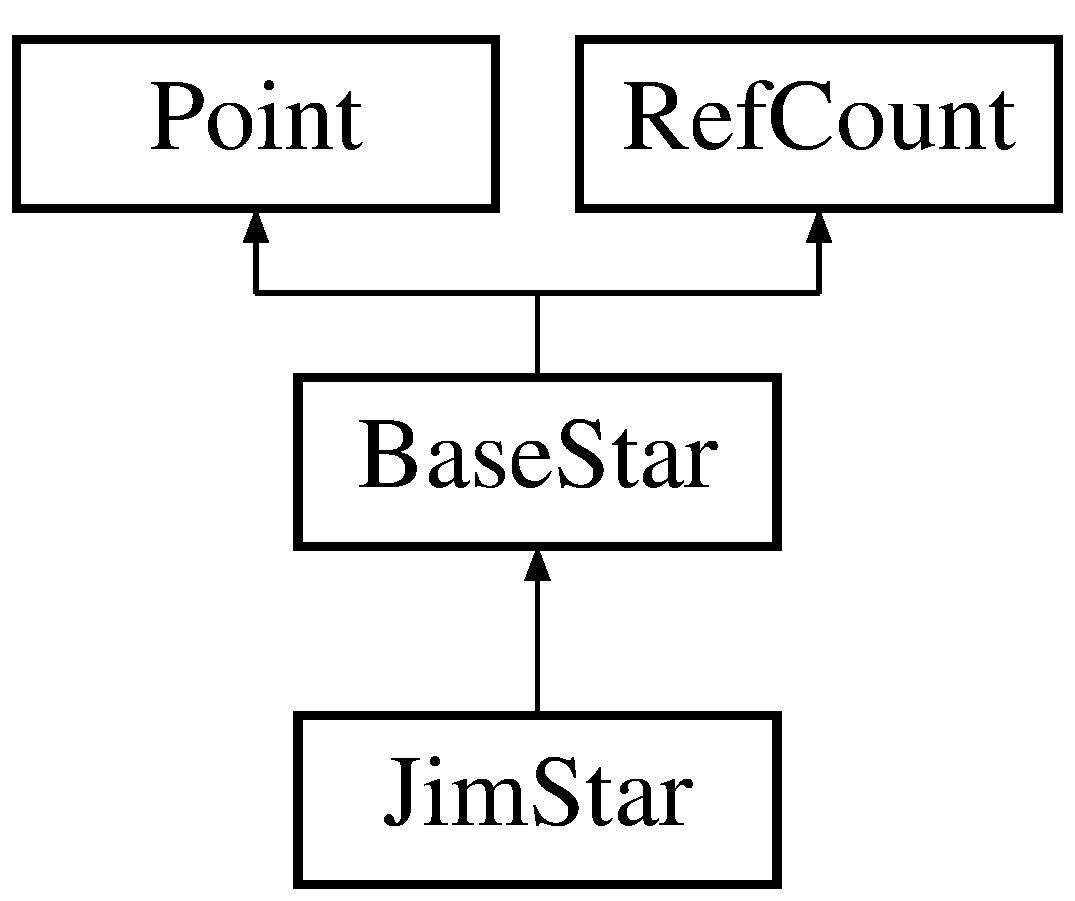
\includegraphics[height=3cm]{class_jimstar}
\end{center}
\end{figure}
\subsubsection*{Public Methods}
\begin{CompactItemize}
\item 
\index{JimStar@{JimStar}!JimStar@{Jim\-Star}}\index{JimStar@{JimStar}!JimStar@{Jim\-Star}}
{\bf Jim\-Star} ()\label{class_jimstar_a0}

\item 
\index{JimStar@{JimStar}!JimStar@{Jim\-Star}}\index{JimStar@{JimStar}!JimStar@{Jim\-Star}}
{\bf Jim\-Star} (double xx, double yy, double ff)\label{class_jimstar_a1}

\item 
\index{Name@{Name}!JimStar@{Jim\-Star}}\index{JimStar@{JimStar}!Name@{Name}}
string {\bf Name} () const\label{class_jimstar_a2}

\item 
\index{Ra@{Ra}!JimStar@{Jim\-Star}}\index{JimStar@{JimStar}!Ra@{Ra}}
double {\bf Ra} () const\label{class_jimstar_a3}

\item 
\index{Dec@{Dec}!JimStar@{Jim\-Star}}\index{JimStar@{JimStar}!Dec@{Dec}}
double {\bf Dec} () const\label{class_jimstar_a4}

\item 
\index{Imag@{Imag}!JimStar@{Jim\-Star}}\index{JimStar@{JimStar}!Imag@{Imag}}
double {\bf Imag} () const\label{class_jimstar_a5}

\item 
\index{Rmag@{Rmag}!JimStar@{Jim\-Star}}\index{JimStar@{JimStar}!Rmag@{Rmag}}
double {\bf Rmag} () const\label{class_jimstar_a6}

\item 
\index{Gmag@{Gmag}!JimStar@{Jim\-Star}}\index{JimStar@{JimStar}!Gmag@{Gmag}}
double {\bf Gmag} () const\label{class_jimstar_a7}

\item 
\index{Zmag@{Zmag}!JimStar@{Jim\-Star}}\index{JimStar@{JimStar}!Zmag@{Zmag}}
double {\bf Zmag} () const\label{class_jimstar_a8}

\item 
\index{Cgal@{Cgal}!JimStar@{Jim\-Star}}\index{JimStar@{JimStar}!Cgal@{Cgal}}
double {\bf Cgal} () const\label{class_jimstar_a9}

\item 
\index{Read@{Read}!JimStar@{Jim\-Star}}\index{JimStar@{JimStar}!Read@{Read}}
virtual void {\bf Read} (istream \&r, const char $\ast$Format)\label{class_jimstar_a10}

\begin{CompactList}\small\item\em to read once the object is created.\item\end{CompactList}\item 
\index{WriteHeader_@{WriteHeader\_\-}!JimStar@{Jim\-Star}}\index{JimStar@{JimStar}!WriteHeader_@{Write\-Header\_\-}}
string {\bf Write\-Header\_\-} (ostream \&pr=cout, const char $\ast$i=NULL) const\label{class_jimstar_a11}

\begin{CompactList}\small\item\em to write the {\bf Star\-List} {\rm (p.\,\pageref{class_starlist})} header with the string appended to every ntuple variable (with no end).\item\end{CompactList}\item 
\index{dumpn@{dumpn}!JimStar@{Jim\-Star}}\index{JimStar@{JimStar}!dumpn@{dumpn}}
virtual void {\bf dumpn} (ostream \&s=cout) const\label{class_jimstar_a12}

\begin{CompactList}\small\item\em for dump with NO end-of-line.\item\end{CompactList}\item 
\index{dump@{dump}!JimStar@{Jim\-Star}}\index{JimStar@{JimStar}!dump@{dump}}
virtual void {\bf dump} (ostream \&s=cout) const\label{class_jimstar_a13}

\begin{CompactList}\small\item\em for dump.\item\end{CompactList}\item 
\index{writen@{writen}!JimStar@{Jim\-Star}}\index{JimStar@{JimStar}!writen@{writen}}
virtual void {\bf writen} (ostream \&s=cout) const\label{class_jimstar_a14}

\begin{CompactList}\small\item\em for write with NO end-of-line.\item\end{CompactList}\item 
\index{write@{write}!JimStar@{Jim\-Star}}\index{JimStar@{JimStar}!write@{write}}
virtual void {\bf write} (ostream \&s=cout) const\label{class_jimstar_a15}

\begin{CompactList}\small\item\em for write.\item\end{CompactList}\end{CompactItemize}
\subsubsection*{Static Public Methods}
\begin{CompactItemize}
\item 
\index{read@{read}!JimStar@{Jim\-Star}}\index{JimStar@{JimStar}!read@{read}}
Jim\-Star$\ast$ {\bf read} (istream \&r, const char $\ast$Format)\label{class_jimstar_d0}

\begin{CompactList}\small\item\em to read and create the object.\item\end{CompactList}\end{CompactItemize}
\subsubsection*{Protected Attributes}
\begin{CompactItemize}
\item 
\index{name@{name}!JimStar@{Jim\-Star}}\index{JimStar@{JimStar}!name@{name}}
string {\bf name}\label{class_jimstar_n0}

\item 
\index{ra@{ra}!JimStar@{Jim\-Star}}\index{JimStar@{JimStar}!ra@{ra}}
double {\bf ra}\label{class_jimstar_n1}

\item 
\index{dec@{dec}!JimStar@{Jim\-Star}}\index{JimStar@{JimStar}!dec@{dec}}
double {\bf dec}\label{class_jimstar_n2}

\item 
\index{imag@{imag}!JimStar@{Jim\-Star}}\index{JimStar@{JimStar}!imag@{imag}}
double {\bf imag}\label{class_jimstar_n3}

\item 
\index{rmag@{rmag}!JimStar@{Jim\-Star}}\index{JimStar@{JimStar}!rmag@{rmag}}
double {\bf rmag}\label{class_jimstar_n4}

\item 
\index{gmag@{gmag}!JimStar@{Jim\-Star}}\index{JimStar@{JimStar}!gmag@{gmag}}
double {\bf gmag}\label{class_jimstar_n5}

\item 
\index{zmag@{zmag}!JimStar@{Jim\-Star}}\index{JimStar@{JimStar}!zmag@{zmag}}
double {\bf zmag}\label{class_jimstar_n6}

\item 
\index{cgal@{cgal}!JimStar@{Jim\-Star}}\index{JimStar@{JimStar}!cgal@{cgal}}
double {\bf cgal}\label{class_jimstar_n7}

\end{CompactItemize}


\subsubsection{Detailed Description}
Jim Calibration Star.

To match an image with the catalogue of Jim  format: ra dec i r g z cgal (cgal=0 ==$>$ etoile) 



The documentation for this class was generated from the following file:\begin{CompactItemize}
\item 
{\bf jimstar.h}\end{CompactItemize}

\subsection{Kernel  Class Reference}
\label{class_kernel}\index{Kernel@{Kernel}}
An odd size {\bf DImage} {\rm (p.\,\pageref{class_dimage})} addressed with (0,0) at center allows quick computation of convolution like operations. 


{\tt \#include $<$dimage.h$>$}

Inheritance diagram for Kernel::\begin{figure}[H]
\begin{center}
\leavevmode
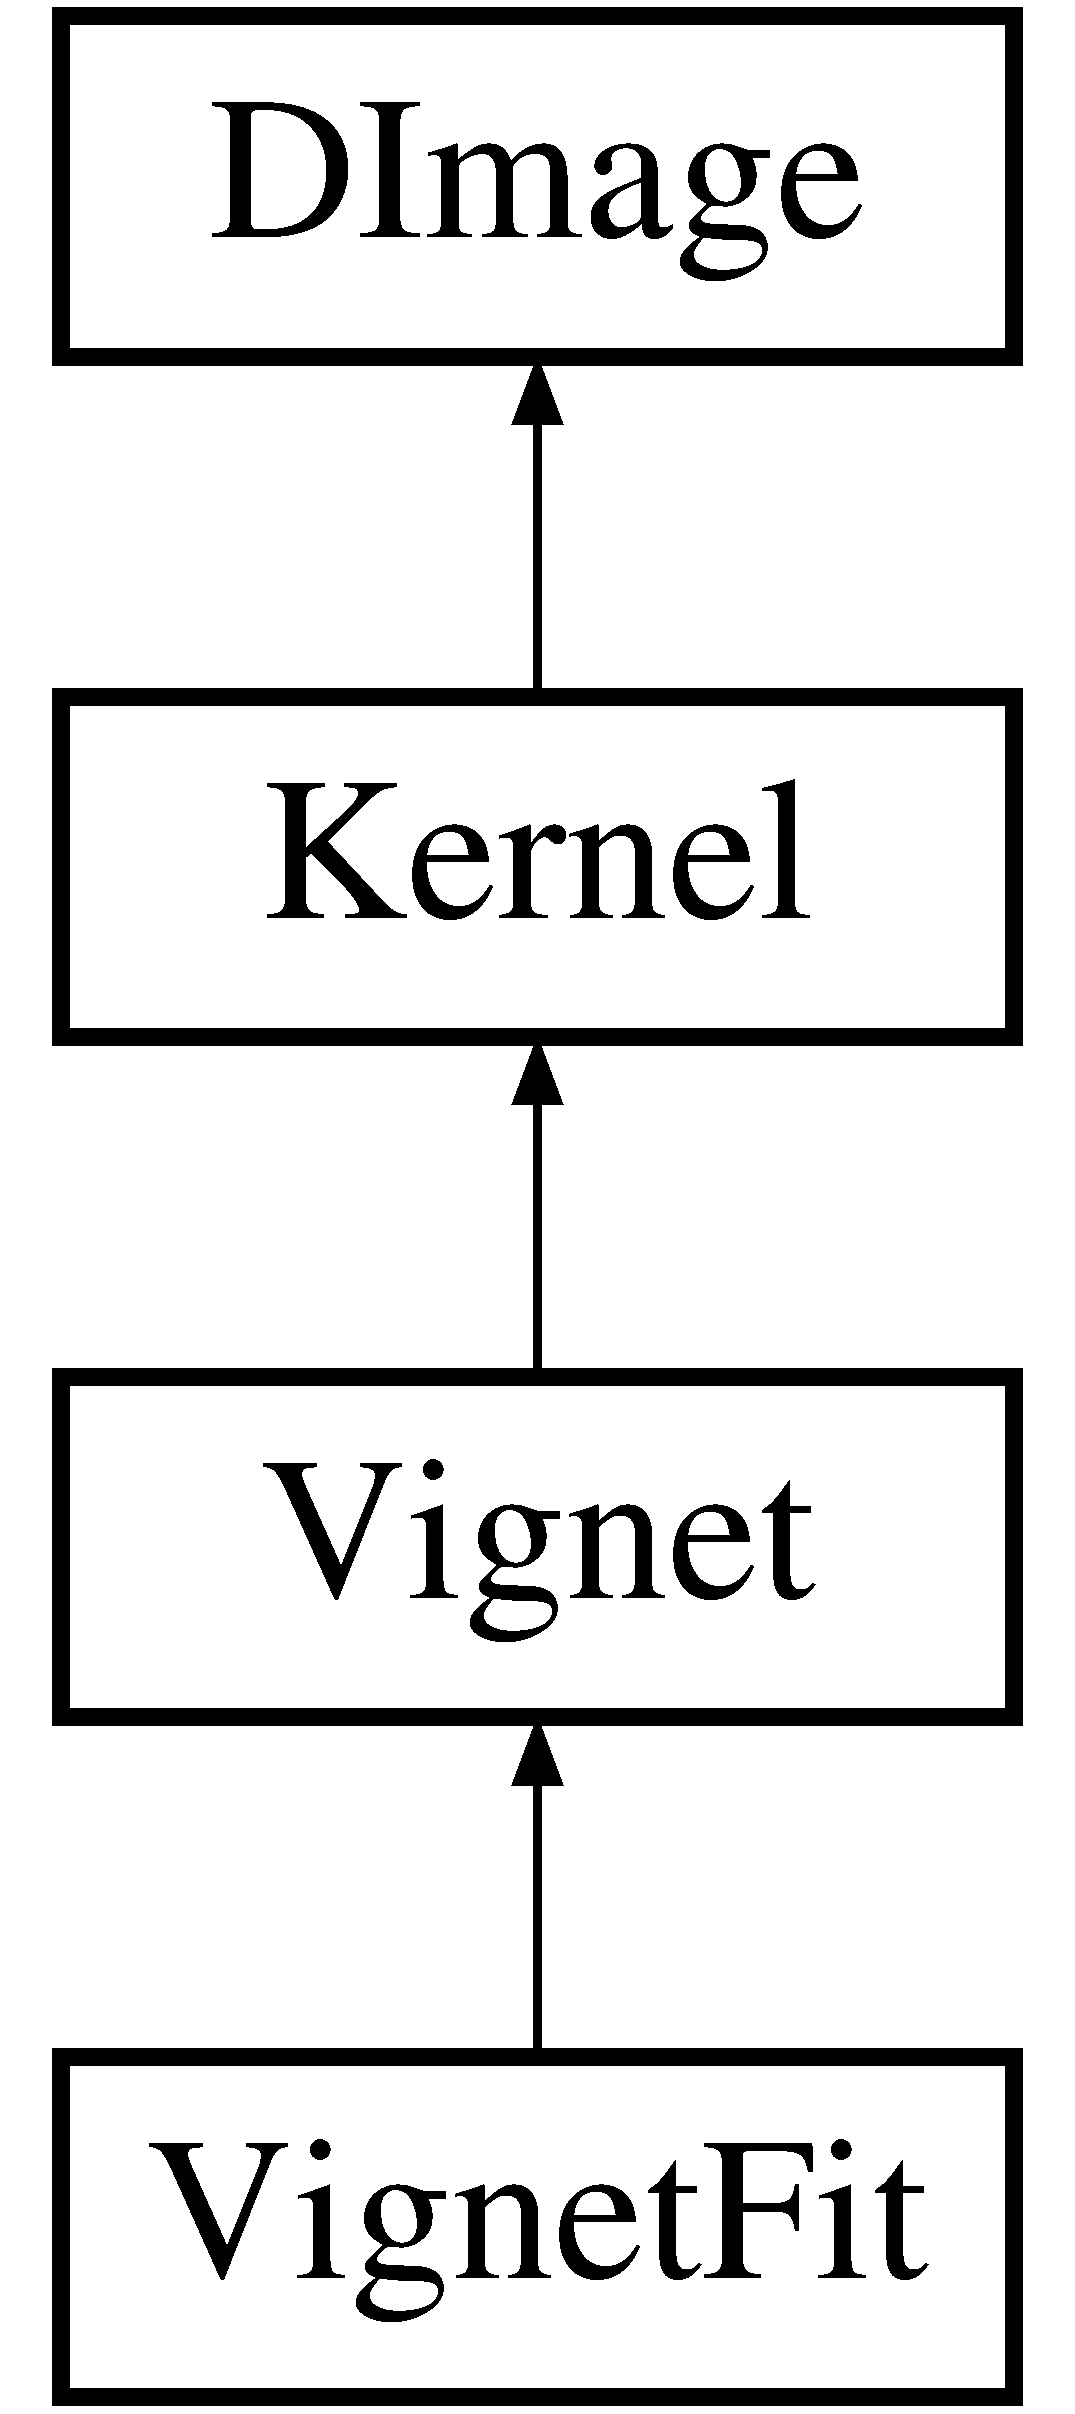
\includegraphics[height=4cm]{class_kernel}
\end{center}
\end{figure}
\subsubsection*{Public Methods}
\begin{CompactItemize}
\item 
\index{Kernel@{Kernel}!Kernel@{Kernel}}\index{Kernel@{Kernel}!Kernel@{Kernel}}
{\bf Kernel} (const int HSize)\label{class_kernel_a0}

\begin{CompactList}\small\item\em construtor for a square kernel of half size Hsize.\item\end{CompactList}\item 
\index{Kernel@{Kernel}!Kernel@{Kernel}}\index{Kernel@{Kernel}!Kernel@{Kernel}}
{\bf Kernel} (const int HSize\-X, const int HSize\-Y)\label{class_kernel_a1}

\begin{CompactList}\small\item\em construtor for a rectangle kernel of half sizes Hsize\-X and Hsize\-Y.\item\end{CompactList}\item 
\index{Kernel@{Kernel}!Kernel@{Kernel}}\index{Kernel@{Kernel}!Kernel@{Kernel}}
{\bf Kernel} (const {\bf DImage} \&Dim)\label{class_kernel_a2}

\item 
\index{Kernel@{Kernel}!Kernel@{Kernel}}\index{Kernel@{Kernel}!Kernel@{Kernel}}
{\bf Kernel} (const string \&Fits\-Name)\label{class_kernel_a3}

\item 
\index{Kernel@{Kernel}!Kernel@{Kernel}}\index{Kernel@{Kernel}!Kernel@{Kernel}}
{\bf Kernel} (const Kernel \&K, int Band\-X, int Band\-Y)\label{class_kernel_a4}

\begin{CompactList}\small\item\em builds a bigger kernel than a given one, and sets extra pixels in the surrounding band to zero.\item\end{CompactList}\item 
\index{Kernel@{Kernel}!Kernel@{Kernel}}\index{Kernel@{Kernel}!Kernel@{Kernel}}
{\bf Kernel} (const Kernel \&Other)\label{class_kernel_a5}

\item 
\index{Kernel@{Kernel}!Kernel@{Kernel}}\index{Kernel@{Kernel}!Kernel@{Kernel}}
{\bf Kernel} ()\label{class_kernel_a6}

\item 
\index{operator=@{operator=}!Kernel@{Kernel}}\index{Kernel@{Kernel}!operator=@{operator=}}
Kernel\& {\bf operator=} (const Kernel \&Right)\label{class_kernel_a7}

\item 
\index{readFits@{readFits}!Kernel@{Kernel}}\index{Kernel@{Kernel}!readFits@{read\-Fits}}
void {\bf read\-Fits} (const string \&Fits\-Name)\label{class_kernel_a8}

\begin{CompactList}\small\item\em write and read the {\bf DImage} {\rm (p.\,\pageref{class_dimage})} as a FITS array.\item\end{CompactList}\item 
\index{IsDirac@{IsDirac}!Kernel@{Kernel}}\index{Kernel@{Kernel}!IsDirac@{Is\-Dirac}}
bool {\bf Is\-Dirac} () const\label{class_kernel_a9}

\item 
\index{HSizeX@{HSizeX}!Kernel@{Kernel}}\index{Kernel@{Kernel}!HSizeX@{HSize\-X}}
int {\bf HSize\-X} () const\label{class_kernel_a10}

\begin{CompactList}\small\item\em half the size in x direction.\item\end{CompactList}\item 
\index{HSizeY@{HSizeY}!Kernel@{Kernel}}\index{Kernel@{Kernel}!HSizeY@{HSize\-Y}}
int {\bf HSize\-Y} () const\label{class_kernel_a11}

\begin{CompactList}\small\item\em half the size in y direction.\item\end{CompactList}\item 
\index{KeepCircleOnly@{KeepCircleOnly}!Kernel@{Kernel}}\index{Kernel@{Kernel}!KeepCircleOnly@{Keep\-Circle\-Only}}
void {\bf Keep\-Circle\-Only} (const double \&radius)\label{class_kernel_a12}

\begin{CompactList}\small\item\em zero out outside a given radius.\item\end{CompactList}\item 
\index{FillWithGaussian@{FillWithGaussian}!Kernel@{Kernel}}\index{Kernel@{Kernel}!FillWithGaussian@{Fill\-With\-Gaussian}}
void {\bf Fill\-With\-Gaussian} (const double \&xc, const double \&yc, const double \&sigmax, const double \&sigmay, const double \&rho=0)\label{class_kernel_a13}

\begin{CompactList}\small\item\em fills the kernel array with a 2d normalized gaussian (xc and yc are in kernel coordinates).\item\end{CompactList}\item 
\index{dump@{dump}!Kernel@{Kernel}}\index{Kernel@{Kernel}!dump@{dump}}
void {\bf dump} () const\label{class_kernel_a14}

\begin{CompactList}\small\item\em prints all kernel values.\item\end{CompactList}\item 
\index{bias@{bias}!Kernel@{Kernel}}\index{Kernel@{Kernel}!bias@{bias}}
void {\bf bias} (double \&x, double \&y) const\label{class_kernel_a15}

\begin{CompactList}\small\item\em computes mean of the kernel on (x,y).\item\end{CompactList}\item 
\index{dump_info@{dump\_\-info}!Kernel@{Kernel}}\index{Kernel@{Kernel}!dump_info@{dump\_\-info}}
void {\bf dump\_\-info} (ostream \&stream=cout) const\label{class_kernel_a16}

\begin{CompactList}\small\item\em prints bias and moments of the kernel.\item\end{CompactList}\item 
\index{moments@{moments}!Kernel@{Kernel}}\index{Kernel@{Kernel}!moments@{moments}}
void {\bf moments} (double \&vx, double \&vy, double \&vxy) const\label{class_kernel_a17}

\begin{CompactList}\small\item\em computes x and y first order moments of the kernel ($\backslash$sigma\_\-x, $\backslash$sigma\_\-y, $\backslash$rho\_\-\{xy\}).\item\end{CompactList}\item 
\index{IsEmpty@{IsEmpty}!Kernel@{Kernel}}\index{Kernel@{Kernel}!IsEmpty@{Is\-Empty}}
bool {\bf Is\-Empty} () const\label{class_kernel_a18}

\item 
\index{MaxPixel@{MaxPixel}!Kernel@{Kernel}}\index{Kernel@{Kernel}!MaxPixel@{Max\-Pixel}}
void {\bf Max\-Pixel} (double \&xmax, double \&ymax)\label{class_kernel_a19}

\item 
\index{MinPixel@{MinPixel}!Kernel@{Kernel}}\index{Kernel@{Kernel}!MinPixel@{Min\-Pixel}}
void {\bf Min\-Pixel} (double \&xmin, double \&ymin)\label{class_kernel_a20}

\end{CompactItemize}
\subsubsection*{Protected Attributes}
\begin{CompactItemize}
\item 
\index{hSizeX@{hSizeX}!Kernel@{Kernel}}\index{Kernel@{Kernel}!hSizeX@{h\-Size\-X}}
int {\bf h\-Size\-X}\label{class_kernel_n0}

\item 
\index{hSizeY@{hSizeY}!Kernel@{Kernel}}\index{Kernel@{Kernel}!hSizeY@{h\-Size\-Y}}
int {\bf h\-Size\-Y}\label{class_kernel_n1}

\end{CompactItemize}


\subsubsection{Detailed Description}
An odd size {\bf DImage} {\rm (p.\,\pageref{class_dimage})} addressed with (0,0) at center allows quick computation of convolution like operations.



The documentation for this class was generated from the following file:\begin{CompactItemize}
\item 
{\bf dimage.h}\end{CompactItemize}

\subsection{Kernel\-Fit  Class Reference}
\label{class_kernelfit}\index{KernelFit@{Kernel\-Fit}}
{\bf Kernel} {\rm (p.\,\pageref{class_kernel})} fitting by least squares. 


{\tt \#include $<$kernelfit.h$>$}

\subsubsection*{Public Methods}
\begin{CompactItemize}
\item 
\index{HKernelSizeX@{HKernelSizeX}!KernelFit@{Kernel\-Fit}}\index{KernelFit@{KernelFit}!HKernelSizeX@{HKernel\-Size\-X}}
int {\bf HKernel\-Size\-X} ()\label{class_kernelfit_a0}

\item 
\index{HKernelSizeY@{HKernelSizeY}!KernelFit@{Kernel\-Fit}}\index{KernelFit@{KernelFit}!HKernelSizeY@{HKernel\-Size\-Y}}
int {\bf HKernel\-Size\-Y} ()\label{class_kernelfit_a1}

\item 
\index{KernIndex@{KernIndex}!KernelFit@{Kernel\-Fit}}\index{KernelFit@{KernelFit}!KernIndex@{Kern\-Index}}
int {\bf Kern\-Index} (int i\-Kernel, int i\-Spatial) const\label{class_kernelfit_a2}

\item 
\index{BackIndex@{BackIndex}!KernelFit@{Kernel\-Fit}}\index{KernelFit@{KernelFit}!BackIndex@{Back\-Index}}
int {\bf Back\-Index} (int ib) const\label{class_kernelfit_a3}

\item 
\index{BackValue@{BackValue}!KernelFit@{Kernel\-Fit}}\index{KernelFit@{KernelFit}!BackValue@{Back\-Value}}
double {\bf Back\-Value} (const double \&x, const double \&y) const\label{class_kernelfit_a4}

\item 
\index{DeleteConvolvedBest@{DeleteConvolvedBest}!KernelFit@{Kernel\-Fit}}\index{KernelFit@{KernelFit}!DeleteConvolvedBest@{Delete\-Convolved\-Best}}
void {\bf Delete\-Convolved\-Best} ()\label{class_kernelfit_a5}

\item 
\index{KernelFit@{KernelFit}!KernelFit@{Kernel\-Fit}}\index{KernelFit@{KernelFit}!KernelFit@{Kernel\-Fit}}
{\bf Kernel\-Fit} ()\label{class_kernelfit_a6}

\item 
\index{~KernelFit@{$\sim$KernelFit}!KernelFit@{Kernel\-Fit}}\index{KernelFit@{KernelFit}!~KernelFit@{$\sim$Kernel\-Fit}}
{\bf $\sim$Kernel\-Fit} ()\label{class_kernelfit_a7}

\item 
\index{KernelsFill@{KernelsFill}!KernelFit@{Kernel\-Fit}}\index{KernelFit@{KernelFit}!KernelsFill@{Kernels\-Fill}}
void {\bf Kernels\-Fill} ()\label{class_kernelfit_a8}

\item 
\index{AllocateConvolvedStamps@{AllocateConvolvedStamps}!KernelFit@{Kernel\-Fit}}\index{KernelFit@{KernelFit}!AllocateConvolvedStamps@{Allocate\-Convolved\-Stamps}}
void {\bf Allocate\-Convolved\-Stamps} ()\label{class_kernelfit_a9}

\item 
\index{DeallocateConvolvedStamps@{DeallocateConvolvedStamps}!KernelFit@{Kernel\-Fit}}\index{KernelFit@{KernelFit}!DeallocateConvolvedStamps@{Deallocate\-Convolved\-Stamps}}
void {\bf Deallocate\-Convolved\-Stamps} ()\label{class_kernelfit_a10}

\item 
\index{ComputeMAndB@{ComputeMAndB}!KernelFit@{Kernel\-Fit}}\index{KernelFit@{KernelFit}!ComputeMAndB@{Compute\-MAnd\-B}}
void {\bf Compute\-MAnd\-B} ()\label{class_kernelfit_a11}

\begin{CompactList}\small\item\em sums least square matrix and vector for all stamps.\item\end{CompactList}\item 
\index{OneStampMAndB@{OneStampMAndB}!KernelFit@{Kernel\-Fit}}\index{KernelFit@{KernelFit}!OneStampMAndB@{One\-Stamp\-MAnd\-B}}
void {\bf One\-Stamp\-MAnd\-B} (const {\bf Stamp} \&Astamp, double $\ast$Stamp\-M, double $\ast$Stamp\-B)\label{class_kernelfit_a12}

\begin{CompactList}\small\item\em computes least square matrix and vector for one stamp.\item\end{CompactList}\item 
\index{SubtractStampFromMAndB@{SubtractStampFromMAndB}!KernelFit@{Kernel\-Fit}}\index{KernelFit@{KernelFit}!SubtractStampFromMAndB@{Subtract\-Stamp\-From\-MAnd\-B}}
void {\bf Subtract\-Stamp\-From\-MAnd\-B} ({\bf Stamp} \&AStamp)\label{class_kernelfit_a13}

\begin{CompactList}\small\item\em subtract a stamp of the least square matrix and vector.\item\end{CompactList}\item 
\index{Solve@{Solve}!KernelFit@{Kernel\-Fit}}\index{KernelFit@{KernelFit}!Solve@{Solve}}
int {\bf Solve} ()\label{class_kernelfit_a14}

\begin{CompactList}\small\item\em actually solves the system by calling linear algebra efficient routines.\item\end{CompactList}\item 
\index{StampChi2@{StampChi2}!KernelFit@{Kernel\-Fit}}\index{KernelFit@{KernelFit}!StampChi2@{Stamp\-Chi2}}
double {\bf Stamp\-Chi2} ({\bf Stamp} \&stamp, double VSky, double Inv\-Gain)\label{class_kernelfit_a15}

\item 
\index{NStampsUsed@{NStampsUsed}!KernelFit@{Kernel\-Fit}}\index{KernelFit@{KernelFit}!NStampsUsed@{NStamps\-Used}}
int {\bf NStamps\-Used} () const\label{class_kernelfit_a16}

\item 
\index{FilterStamps@{FilterStamps}!KernelFit@{Kernel\-Fit}}\index{KernelFit@{KernelFit}!FilterStamps@{Filter\-Stamps}}
void {\bf Filter\-Stamps} ()\label{class_kernelfit_a17}

\item 
int {\bf Do\-The\-Fit} (const Base\-Star\-List \&List, double \&Best\-Seeing, double \&Worst\-Seeing)
\begin{CompactList}\small\item\em final wrapper that calls various routines to fill matrix and vector, and then solve.\item\end{CompactList}\item 
\index{DoIt@{DoIt}!KernelFit@{Kernel\-Fit}}\index{KernelFit@{KernelFit}!DoIt@{Do\-It}}
int {\bf Do\-It} (const Base\-Star\-List \&List, double \&Best\-Seeing, double \&Worst\-Seeing)\label{class_kernelfit_a19}

\begin{CompactList}\small\item\em does the kernel fit (Do\-The\-Fit) and the convolution (Best\-Image\-Convolve).\item\end{CompactList}\item 
\index{KernCompute@{KernCompute}!KernelFit@{Kernel\-Fit}}\index{KernelFit@{KernelFit}!KernCompute@{Kern\-Compute}}
void {\bf Kern\-Compute} ({\bf Kernel} \&Result, const double X, const double Y) const\label{class_kernelfit_a20}

\item 
void {\bf Best\-Image\-Convolve} (int Update\-Kern\-Step=100)
\begin{CompactList}\small\item\em convolves the best image with the current kernel (Usually set by Do\-The\-Fit).\item\end{CompactList}\item 
\index{VarianceConvolve@{VarianceConvolve}!KernelFit@{Kernel\-Fit}}\index{KernelFit@{KernelFit}!VarianceConvolve@{Variance\-Convolve}}
{\bf Image}$\ast$ {\bf Variance\-Convolve} (const {\bf Image} \&Source, int Update\-Kern=100)\label{class_kernelfit_a22}

\end{CompactItemize}
\subsubsection*{Public Attributes}
\begin{CompactItemize}
\item 
\index{BestImage@{BestImage}!KernelFit@{Kernel\-Fit}}\index{KernelFit@{KernelFit}!BestImage@{Best\-Image}}
const {\bf Image}$\ast$ {\bf Best\-Image}\label{class_kernelfit_m0}

\begin{CompactList}\small\item\em pointer to 'best' image (smaller seeing).\item\end{CompactList}\item 
\index{WorstImage@{WorstImage}!KernelFit@{Kernel\-Fit}}\index{KernelFit@{KernelFit}!WorstImage@{Worst\-Image}}
const {\bf Image}$\ast$ {\bf Worst\-Image}\label{class_kernelfit_m1}

\begin{CompactList}\small\item\em pointer to 'worst' image (larger seeing).\item\end{CompactList}\item 
\index{BestImageBack@{BestImageBack}!KernelFit@{Kernel\-Fit}}\index{KernelFit@{KernelFit}!BestImageBack@{Best\-Image\-Back}}
double {\bf Best\-Image\-Back}\label{class_kernelfit_m2}

\begin{CompactList}\small\item\em the value of the sky of the best image.\item\end{CompactList}\item 
\index{WorstImageBack@{WorstImageBack}!KernelFit@{Kernel\-Fit}}\index{KernelFit@{KernelFit}!WorstImageBack@{Worst\-Image\-Back}}
double {\bf Worst\-Image\-Back}\label{class_kernelfit_m3}

\begin{CompactList}\small\item\em the value of the sky of the worst image.\item\end{CompactList}\item 
\index{SkyVarianceWorstImage@{SkyVarianceWorstImage}!KernelFit@{Kernel\-Fit}}\index{KernelFit@{KernelFit}!SkyVarianceWorstImage@{Sky\-Variance\-Worst\-Image}}
double {\bf Sky\-Variance\-Worst\-Image}\label{class_kernelfit_m4}

\begin{CompactList}\small\item\em the value of the sky variance of Worst\-Image.\item\end{CompactList}\item 
\index{WorstImageGain@{WorstImageGain}!KernelFit@{Kernel\-Fit}}\index{KernelFit@{KernelFit}!WorstImageGain@{Worst\-Image\-Gain}}
double {\bf Worst\-Image\-Gain}\label{class_kernelfit_m5}

\begin{CompactList}\small\item\em the gain of Worst\-Image.\item\end{CompactList}\item 
\index{KernAtCenterSum@{KernAtCenterSum}!KernelFit@{Kernel\-Fit}}\index{KernelFit@{KernelFit}!KernAtCenterSum@{Kern\-At\-Center\-Sum}}
double {\bf Kern\-At\-Center\-Sum}\label{class_kernelfit_m6}

\begin{CompactList}\small\item\em the kernel integral at the image center (photometric ratio).\item\end{CompactList}\item 
\index{Kernels@{Kernels}!KernelFit@{Kernel\-Fit}}\index{KernelFit@{KernelFit}!Kernels@{Kernels}}
vector$<${\bf Kernel}$>$ {\bf Kernels}\label{class_kernelfit_m7}

\item 
{\bf Stamp\-List}$\ast$ {\bf Best\-Image\-Stamps}
\begin{CompactList}\small\item\em the base used to build the 'best' kernel $\ast$/ the list of stamps in the 'best' image.\item\end{CompactList}\item 
\index{ConvolvedBest@{ConvolvedBest}!KernelFit@{Kernel\-Fit}}\index{KernelFit@{KernelFit}!ConvolvedBest@{Convolved\-Best}}
{\bf Image}$\ast$ {\bf Convolved\-Best}\label{class_kernelfit_m9}

\begin{CompactList}\small\item\em a pointer to the 'best' image convolved with the solution.\item\end{CompactList}\item 
\index{convolutions@{convolutions}!KernelFit@{Kernel\-Fit}}\index{KernelFit@{KernelFit}!convolutions@{convolutions}}
{\bf DImage}$\ast$ {\bf convolutions}\label{class_kernelfit_m10}

\item 
\index{backStamps@{backStamps}!KernelFit@{Kernel\-Fit}}\index{KernelFit@{KernelFit}!backStamps@{back\-Stamps}}
{\bf DImage}$\ast$ {\bf back\-Stamps}\label{class_kernelfit_m11}

\item 
\index{optParams@{optParams}!KernelFit@{Kernel\-Fit}}\index{KernelFit@{KernelFit}!optParams@{opt\-Params}}
Opt\-Params {\bf opt\-Params}\label{class_kernelfit_m12}

\item 
\index{mSize@{mSize}!KernelFit@{Kernel\-Fit}}\index{KernelFit@{KernelFit}!mSize@{m\-Size}}
int {\bf m\-Size}\label{class_kernelfit_m13}

\item 
\index{backStart@{backStart}!KernelFit@{Kernel\-Fit}}\index{KernelFit@{KernelFit}!backStart@{back\-Start}}
int {\bf back\-Start}\label{class_kernelfit_m14}

\item 
\index{m@{m}!KernelFit@{Kernel\-Fit}}\index{KernelFit@{KernelFit}!m@{m}}
double$\ast$ {\bf m}\label{class_kernelfit_m15}

\item 
double$\ast$ {\bf b}
\begin{CompactList}\small\item\em the least-squares matrix (the second derivative of chi2 w.r.t fitted parameters $\ast$/;.\item\end{CompactList}\item 
double$\ast$ {\bf solution}
\begin{CompactList}\small\item\em the normal equations (i.e. grad(chi2) = 0) right hand side $\ast$/.\item\end{CompactList}\item 
\index{chi2@{chi2}!KernelFit@{Kernel\-Fit}}\index{KernelFit@{KernelFit}!chi2@{chi2}}
double {\bf chi2}\label{class_kernelfit_m18}

\end{CompactItemize}


\subsubsection{Detailed Description}
{\bf Kernel} {\rm (p.\,\pageref{class_kernel})} fitting by least squares.

Implementation of Ch. Alard's method for fitting (slowly variable)  convolution kernels. see astro-ph 9903111 \& astro-ph 9712287  (where most of the equations of page 2 are wrong). Main differences with the \char`\"{}isis\char`\"{} code provided by Alard himself: \begin{CompactItemize}
\item 
 if the integral of the kernel is requested to be constant over the image, we use Lagrange multipliers instead of something I could not understand. (paper from 97 page 3 first column). \item 
 for the detection of outliers, we compute the chi2 of all stamps,  apply median filtering, refit, and iterate until stabilization of the number of stamps. This is in fact fairly fast because we have routines to  add or remove one stamp from the fit. \end{CompactItemize}




\subsubsection{Member Function Documentation}
\index{KernelFit@{Kernel\-Fit}!BestImageConvolve@{BestImageConvolve}}
\index{BestImageConvolve@{BestImageConvolve}!KernelFit@{Kernel\-Fit}}
\paragraph{\setlength{\rightskip}{0pt plus 5cm}void Kernel\-Fit::Best\-Image\-Convolve (int {\em Update\-Kern} = 100)}\hfill\label{class_kernelfit_a21}


convolves the best image with the current kernel (Usually set by Do\-The\-Fit).

The Update\-Kern parameter is the pixel range over which the kernel will not be updated. The concolved image is to be found in Convolved\-Best. \index{KernelFit@{Kernel\-Fit}!DoTheFit@{DoTheFit}}
\index{DoTheFit@{DoTheFit}!KernelFit@{Kernel\-Fit}}
\paragraph{\setlength{\rightskip}{0pt plus 5cm}int Kernel\-Fit::Do\-The\-Fit (const Base\-Star\-List \& {\em List}, double \& {\em Best\-Seeing}, double \& {\em Worst\-Seeing})}\hfill\label{class_kernelfit_a18}


final wrapper that calls various routines to fill matrix and vector, and then solve.

Before entering here, 'this' should have the Best\-Image and Worst\-Image fields assigned. The various sizes of the stamps involved in kernel fit are computed by Opt\-Params::Optimize\-Sizes(). There is no way yet to by-pass it and setup the fit conditions by yourself (it would be simple to implement). The returned value is 0 if the kernel fit failed (and hence 'this' contains no viable kernel). \begin{Desc}
\item[{\bf Parameters: }]\par
\begin{description}
\item[
{\em List}]contains the stars elligible to fit the kernel. \end{description}
\end{Desc}


\subsubsection{Member Data Documentation}
\index{KernelFit@{Kernel\-Fit}!BestImageStamps@{BestImageStamps}}
\index{BestImageStamps@{BestImageStamps}!KernelFit@{Kernel\-Fit}}
\paragraph{\setlength{\rightskip}{0pt plus 5cm}{\bf Stamp\-List} $\ast$ Kernel\-Fit::Best\-Image\-Stamps}\hfill\label{class_kernelfit_m8}


the base used to build the 'best' kernel $\ast$/ the list of stamps in the 'best' image.

/$\ast$ \index{KernelFit@{Kernel\-Fit}!b@{b}}
\index{b@{b}!KernelFit@{Kernel\-Fit}}
\paragraph{\setlength{\rightskip}{0pt plus 5cm}double $\ast$ Kernel\-Fit::b}\hfill\label{class_kernelfit_m16}


the least-squares matrix (the second derivative of chi2 w.r.t fitted parameters $\ast$/;.

/$\ast$ \index{KernelFit@{Kernel\-Fit}!solution@{solution}}
\index{solution@{solution}!KernelFit@{Kernel\-Fit}}
\paragraph{\setlength{\rightskip}{0pt plus 5cm}double $\ast$ Kernel\-Fit::solution}\hfill\label{class_kernelfit_m17}


the normal equations (i.e. grad(chi2) = 0) right hand side $\ast$/.

/$\ast$ 

The documentation for this class was generated from the following files:\begin{CompactItemize}
\item 
{\bf kernelfit.h}\item 
kernelfit.cc\end{CompactItemize}

\subsection{Light\-Curve  Class Reference}
\label{class_lightcurve}\index{LightCurve@{Light\-Curve}}
The same Fiducial\-Star monitored many nights. 


{\tt \#include $<$lightcurve.h$>$}

Inheritance diagram for Light\-Curve::\begin{figure}[H]
\begin{center}
\leavevmode
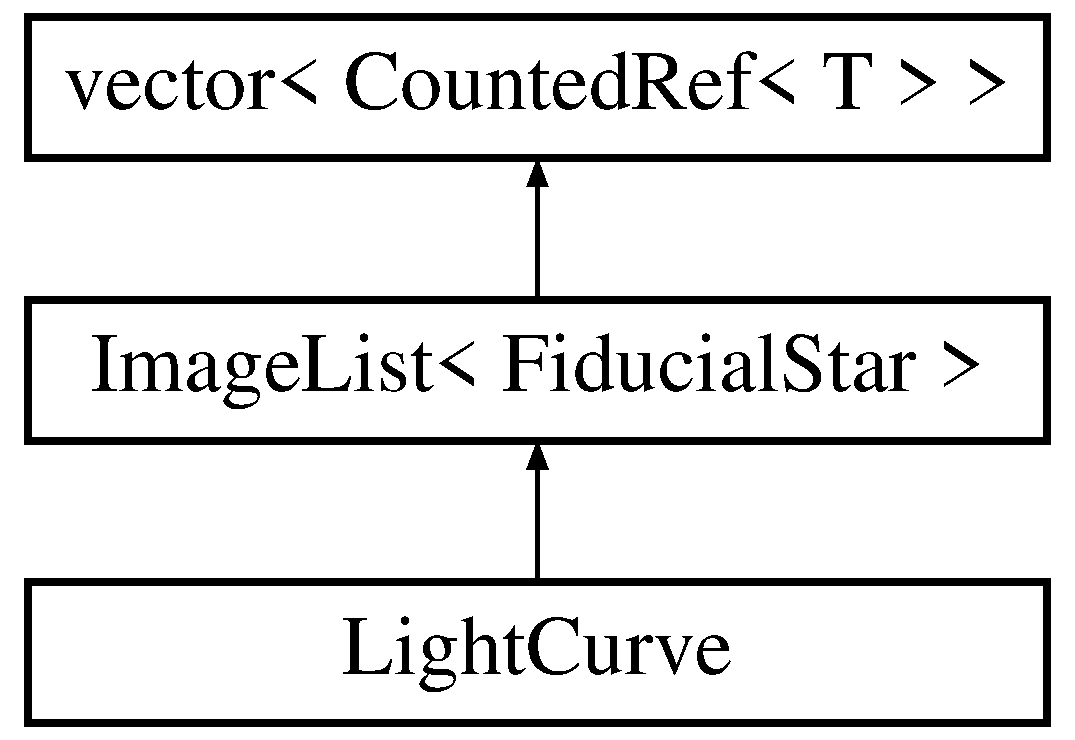
\includegraphics[height=3cm]{class_lightcurve}
\end{center}
\end{figure}
\subsubsection*{Public Methods}
\begin{CompactItemize}
\item 
\index{LightCurve@{LightCurve}!LightCurve@{Light\-Curve}}\index{LightCurve@{LightCurve}!LightCurve@{Light\-Curve}}
{\bf Light\-Curve} (const Night\-List \&All\-Nights, const Phot\-Star \&One\-Star)\label{class_lightcurve_a0}

\item 
\index{LightCurve@{LightCurve}!LightCurve@{Light\-Curve}}\index{LightCurve@{LightCurve}!LightCurve@{Light\-Curve}}
{\bf Light\-Curve} (istream \&Stream)\label{class_lightcurve_a1}

\item 
\index{LightCurve@{LightCurve}!LightCurve@{Light\-Curve}}\index{LightCurve@{LightCurve}!LightCurve@{Light\-Curve}}
{\bf Light\-Curve} ()\label{class_lightcurve_a2}

\item 
\index{AveragePosition@{AveragePosition}!LightCurve@{Light\-Curve}}\index{LightCurve@{LightCurve}!AveragePosition@{Average\-Position}}
void {\bf Average\-Position} ()\label{class_lightcurve_a3}

\begin{CompactList}\small\item\em take the weighted mean of all positions.\item\end{CompactList}\item 
\index{RelativeFluxes@{RelativeFluxes}!LightCurve@{Light\-Curve}}\index{LightCurve@{LightCurve}!RelativeFluxes@{Relative\-Fluxes}}
void {\bf Relative\-Fluxes} ()\label{class_lightcurve_a4}

\begin{CompactList}\small\item\em compute the relative fluxes according to the night photometric ratios.\item\end{CompactList}\item 
\index{AbsoluteFluxes@{AbsoluteFluxes}!LightCurve@{Light\-Curve}}\index{LightCurve@{LightCurve}!AbsoluteFluxes@{Absolute\-Fluxes}}
void {\bf Absolute\-Fluxes} ()\label{class_lightcurve_a5}

\begin{CompactList}\small\item\em compute the absolute calibrated fluxes.\item\end{CompactList}\item 
\index{dump@{dump}!LightCurve@{Light\-Curve}}\index{LightCurve@{LightCurve}!dump@{dump}}
void {\bf dump} (ostream \&Stream=cout) const\label{class_lightcurve_a6}

\item 
\index{write_header@{write\_\-header}!LightCurve@{Light\-Curve}}\index{LightCurve@{LightCurve}!write_header@{write\_\-header}}
void {\bf write\_\-header} (ostream \&Stream) const\label{class_lightcurve_a7}

\item 
\index{write@{write}!LightCurve@{Light\-Curve}}\index{LightCurve@{LightCurve}!write@{write}}
void {\bf write} (ostream \&Stream) const\label{class_lightcurve_a8}

\item 
\index{write@{write}!LightCurve@{Light\-Curve}}\index{LightCurve@{LightCurve}!write@{write}}
void {\bf write} (const string \&File\-Name) const\label{class_lightcurve_a9}

\item 
\index{read@{read}!LightCurve@{Light\-Curve}}\index{LightCurve@{LightCurve}!read@{read}}
void {\bf read} (istream \&Stream)\label{class_lightcurve_a10}

\end{CompactItemize}
\subsubsection*{Public Attributes}
\begin{CompactItemize}
\item 
\index{refstar@{refstar}!LightCurve@{Light\-Curve}}\index{LightCurve@{LightCurve}!refstar@{refstar}}
Phot\-Star {\bf refstar}\label{class_lightcurve_m0}

\item 
\index{IsStandard@{IsStandard}!LightCurve@{Light\-Curve}}\index{LightCurve@{LightCurve}!IsStandard@{Is\-Standard}}
bool {\bf Is\-Standard}\label{class_lightcurve_m1}

\begin{CompactList}\small\item\em returns true if the Fiducial\-Star is a standard star.\item\end{CompactList}\item 
\index{FidName@{FidName}!LightCurve@{Light\-Curve}}\index{LightCurve@{LightCurve}!FidName@{Fid\-Name}}
string {\bf Fid\-Name}\label{class_lightcurve_m2}

\begin{CompactList}\small\item\em name of the star, useful for bookeeping.\item\end{CompactList}\end{CompactItemize}
\subsubsection*{Friends}
\begin{CompactItemize}
\item 
\index{ByIncreasingFlux@{ByIncreasingFlux}!LightCurve@{Light\-Curve}}\index{LightCurve@{LightCurve}!ByIncreasingFlux@{By\-Increasing\-Flux}}
bool {\bf By\-Increasing\-Flux} (const Fiducial\-Star $\ast$one, const Fiducial\-Star $\ast$two)\label{class_lightcurve_l0}

\begin{CompactList}\small\item\em sorts by increasing fluxes.\item\end{CompactList}\item 
\index{ByIncreasingSignalToNoise@{ByIncreasingSignalToNoise}!LightCurve@{Light\-Curve}}\index{LightCurve@{LightCurve}!ByIncreasingSignalToNoise@{By\-Increasing\-Signal\-To\-Noise}}
bool {\bf By\-Increasing\-Signal\-To\-Noise} (const Fiducial\-Star $\ast$one, const Fiducial\-Star $\ast$two)\label{class_lightcurve_l1}

\begin{CompactList}\small\item\em sorts by increasing signal to noise.\item\end{CompactList}\end{CompactItemize}


\subsubsection{Detailed Description}
The same Fiducial\-Star monitored many nights.



The documentation for this class was generated from the following file:\begin{CompactItemize}
\item 
{\bf lightcurve.h}\end{CompactItemize}

\subsection{Light\-Curve\-Builder  Class Reference}
\label{class_lightcurvebuilder}\index{LightCurveBuilder@{Light\-Curve\-Builder}}
Lightcurve builder for one band. Execute different types of photometry. 


{\tt \#include $<$lightcurvebuilder.h$>$}

Inheritance diagram for Light\-Curve\-Builder::\begin{figure}[H]
\begin{center}
\leavevmode
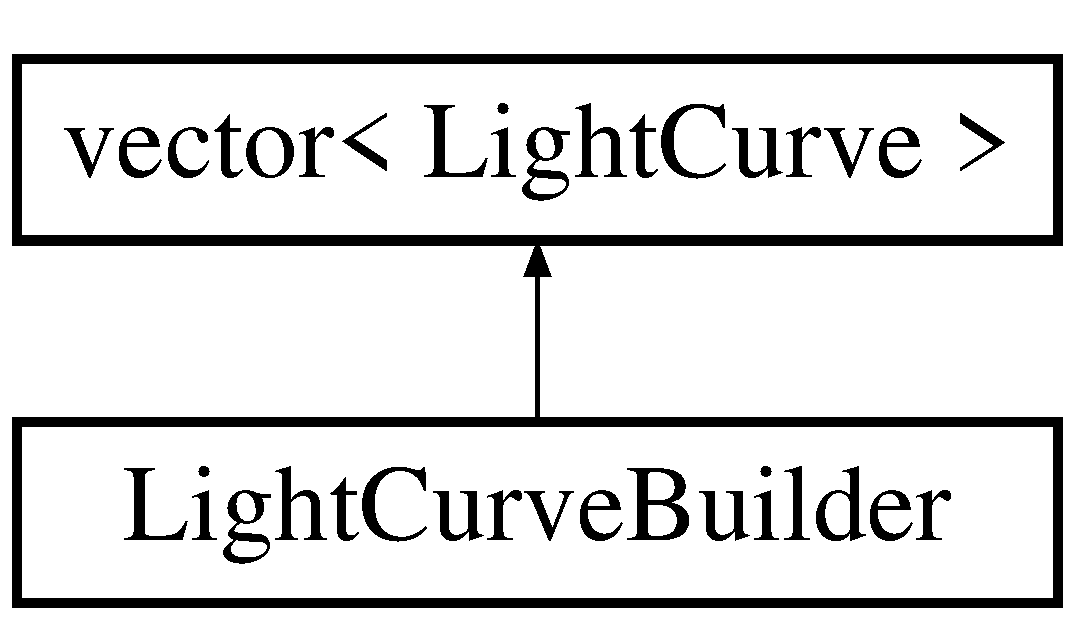
\includegraphics[height=2cm]{class_lightcurvebuilder}
\end{center}
\end{figure}
\subsubsection*{Public Methods}
\begin{CompactItemize}
\item 
\index{LightCurveBuilder@{LightCurveBuilder}!LightCurveBuilder@{Light\-Curve\-Builder}}\index{LightCurveBuilder@{LightCurveBuilder}!LightCurveBuilder@{Light\-Curve\-Builder}}
{\bf Light\-Curve\-Builder} (const Reduced\-Image\-List \&Images)\label{class_lightcurvebuilder_a0}

\begin{CompactList}\small\item\em main constructor.\item\end{CompactList}\item 
\index{LightCurveBuilder@{LightCurveBuilder}!LightCurveBuilder@{Light\-Curve\-Builder}}\index{LightCurveBuilder@{LightCurveBuilder}!LightCurveBuilder@{Light\-Curve\-Builder}}
{\bf Light\-Curve\-Builder} ()\label{class_lightcurvebuilder_a1}

\item 
\index{LightCurveBuilder@{LightCurveBuilder}!LightCurveBuilder@{Light\-Curve\-Builder}}\index{LightCurveBuilder@{LightCurveBuilder}!LightCurveBuilder@{Light\-Curve\-Builder}}
{\bf Light\-Curve\-Builder} (const Light\-Curve\-Builder \&Other)\label{class_lightcurvebuilder_a2}

\begin{CompactList}\small\item\em copy constructor.\item\end{CompactList}\item 
\index{operator=@{operator=}!LightCurveBuilder@{Light\-Curve\-Builder}}\index{LightCurveBuilder@{LightCurveBuilder}!operator=@{operator=}}
Light\-Curve\-Builder\& {\bf operator=} (const Light\-Curve\-Builder \&Right)\label{class_lightcurvebuilder_a3}

\item 
\index{~LightCurveBuilder@{$\sim$LightCurveBuilder}!LightCurveBuilder@{Light\-Curve\-Builder}}\index{LightCurveBuilder@{LightCurveBuilder}!~LightCurveBuilder@{$\sim$Light\-Curve\-Builder}}
{\bf $\sim$Light\-Curve\-Builder} ()\label{class_lightcurvebuilder_a4}

\item 
\index{Calibrate@{Calibrate}!LightCurveBuilder@{Light\-Curve\-Builder}}\index{LightCurveBuilder@{LightCurveBuilder}!Calibrate@{Calibrate}}
void {\bf Calibrate} (const double \&Nfwhm) const\label{class_lightcurvebuilder_a5}

\begin{CompactList}\small\item\em should calibrate properly the lightcurve, but does not.\item\end{CompactList}\item 
\index{Init@{Init}!LightCurveBuilder@{Light\-Curve\-Builder}}\index{LightCurveBuilder@{LightCurveBuilder}!Init@{Init}}
bool {\bf Init} (const vector$<$ {\bf Point} $>$ \&SNe)\label{class_lightcurvebuilder_a6}

\begin{CompactList}\small\item\em init the lightcurve.\item\end{CompactList}\item 
\index{Init@{Init}!LightCurveBuilder@{Light\-Curve\-Builder}}\index{LightCurveBuilder@{LightCurveBuilder}!Init@{Init}}
bool {\bf Init} (const vector$<$ {\bf Point} $>$ \&SNe, const string \&catalogue)\label{class_lightcurvebuilder_a7}

\begin{CompactList}\small\item\em init the lightcurve with a catalogue of standard stars.\item\end{CompactList}\item 
\index{InitFiducials@{InitFiducials}!LightCurveBuilder@{Light\-Curve\-Builder}}\index{LightCurveBuilder@{LightCurveBuilder}!InitFiducials@{Init\-Fiducials}}
void {\bf Init\-Fiducials} (const Base\-Star\-List \&Fid\-List)\label{class_lightcurvebuilder_a8}

\begin{CompactList}\small\item\em init all common objects.\item\end{CompactList}\item 
\index{StarListPhotometry@{StarListPhotometry}!LightCurveBuilder@{Light\-Curve\-Builder}}\index{LightCurveBuilder@{LightCurveBuilder}!StarListPhotometry@{Star\-List\-Photometry}}
void {\bf Star\-List\-Photometry} ()\label{class_lightcurvebuilder_a9}

\begin{CompactList}\small\item\em performs a quick photometry from the starlists.\item\end{CompactList}\item 
\index{SubAperPhotometry@{SubAperPhotometry}!LightCurveBuilder@{Light\-Curve\-Builder}}\index{LightCurveBuilder@{LightCurveBuilder}!SubAperPhotometry@{Sub\-Aper\-Photometry}}
void {\bf Sub\-Aper\-Photometry} (const double \&Nfwhm)\label{class_lightcurvebuilder_a10}

\begin{CompactList}\small\item\em performs aperture photometry on the subtractions.\item\end{CompactList}\item 
\index{BuildKernelsAndSubs@{BuildKernelsAndSubs}!LightCurveBuilder@{Light\-Curve\-Builder}}\index{LightCurveBuilder@{LightCurveBuilder}!BuildKernelsAndSubs@{Build\-Kernels\-And\-Subs}}
void {\bf Build\-Kernels\-And\-Subs} ()\label{class_lightcurvebuilder_a11}

\begin{CompactList}\small\item\em build the kernels among the reference and the other images.\item\end{CompactList}\item 
\index{SimFitPhotometry@{SimFitPhotometry}!LightCurveBuilder@{Light\-Curve\-Builder}}\index{LightCurveBuilder@{LightCurveBuilder}!SimFitPhotometry@{Sim\-Fit\-Photometry}}
void {\bf Sim\-Fit\-Photometry} ()\label{class_lightcurvebuilder_a12}

\begin{CompactList}\small\item\em performs simultaneous photometry for each lightcurve star.\item\end{CompactList}\item 
\index{write@{write}!LightCurveBuilder@{Light\-Curve\-Builder}}\index{LightCurveBuilder@{LightCurveBuilder}!write@{write}}
void {\bf write} (const string \&Middle\-Name) const\label{class_lightcurvebuilder_a13}

\begin{CompactList}\small\item\em write something.\item\end{CompactList}\end{CompactItemize}
\subsubsection*{Public Attributes}
\begin{CompactItemize}
\item 
\index{Reference@{Reference}!LightCurveBuilder@{Light\-Curve\-Builder}}\index{LightCurveBuilder@{LightCurveBuilder}!Reference@{Reference}}
{\bf Night}$\ast$ {\bf Reference}\label{class_lightcurvebuilder_m0}

\begin{CompactList}\small\item\em a pointer to the reference night.\item\end{CompactList}\item 
\index{Nights@{Nights}!LightCurveBuilder@{Light\-Curve\-Builder}}\index{LightCurveBuilder@{LightCurveBuilder}!Nights@{Nights}}
Night\-List {\bf Nights}\label{class_lightcurvebuilder_m1}

\begin{CompactList}\small\item\em the list of images where each lightcurve point is refered.\item\end{CompactList}\item 
\index{BandName@{BandName}!LightCurveBuilder@{Light\-Curve\-Builder}}\index{LightCurveBuilder@{LightCurveBuilder}!BandName@{Band\-Name}}
string {\bf Band\-Name}\label{class_lightcurvebuilder_m2}

\begin{CompactList}\small\item\em a band name associated with this list.\item\end{CompactList}\item 
\index{nsn@{nsn}!LightCurveBuilder@{Light\-Curve\-Builder}}\index{LightCurveBuilder@{LightCurveBuilder}!nsn@{nsn}}
unsigned {\bf nsn}\label{class_lightcurvebuilder_m3}

\begin{CompactList}\small\item\em the number of supernovae.\item\end{CompactList}\end{CompactItemize}


\subsubsection{Detailed Description}
Lightcurve builder for one band. Execute different types of photometry.



The documentation for this class was generated from the following file:\begin{CompactItemize}
\item 
{\bf lightcurvebuilder.h}\end{CompactItemize}

\subsection{Light\-Curve\-Guru  Class Reference}
\label{class_lightcurveguru}\index{LightCurveGuru@{Light\-Curve\-Guru}}
Main lightcurve builder for all bands. 


{\tt \#include $<$lightcurveguru.h$>$}

\subsubsection*{Public Methods}
\begin{CompactItemize}
\item 
\index{LightCurveGuru@{LightCurveGuru}!LightCurveGuru@{Light\-Curve\-Guru}}\index{LightCurveGuru@{LightCurveGuru}!LightCurveGuru@{Light\-Curve\-Guru}}
{\bf Light\-Curve\-Guru} ()\label{class_lightcurveguru_a0}

\item 
\index{~LightCurveGuru@{$\sim$LightCurveGuru}!LightCurveGuru@{Light\-Curve\-Guru}}\index{LightCurveGuru@{LightCurveGuru}!~LightCurveGuru@{$\sim$Light\-Curve\-Guru}}
{\bf $\sim$Light\-Curve\-Guru} ()\label{class_lightcurveguru_a1}

\item 
\index{read@{read}!LightCurveGuru@{Light\-Curve\-Guru}}\index{LightCurveGuru@{LightCurveGuru}!read@{read}}
bool {\bf read} (const string \&File\-Name)\label{class_lightcurveguru_a2}

\begin{CompactList}\small\item\em read initial lightcurve file.\item\end{CompactList}\item 
\index{MakeNights@{MakeNights}!LightCurveGuru@{Light\-Curve\-Guru}}\index{LightCurveGuru@{LightCurveGuru}!MakeNights@{Make\-Nights}}
bool {\bf Make\-Nights} ()\label{class_lightcurveguru_a3}

\begin{CompactList}\small\item\em check, align and stack images night by night, instrument by instrument, band by band.\item\end{CompactList}\item 
\index{SelectFidRef@{SelectFidRef}!LightCurveGuru@{Light\-Curve\-Guru}}\index{LightCurveGuru@{LightCurveGuru}!SelectFidRef@{Select\-Fid\-Ref}}
bool {\bf Select\-Fid\-Ref} ()\label{class_lightcurveguru_a4}

\begin{CompactList}\small\item\em select a fiducial reference lightcurve list.\item\end{CompactList}\item 
\index{MatchFiducials@{MatchFiducials}!LightCurveGuru@{Light\-Curve\-Guru}}\index{LightCurveGuru@{LightCurveGuru}!MatchFiducials@{Match\-Fiducials}}
bool {\bf Match\-Fiducials} ()\label{class_lightcurveguru_a5}

\begin{CompactList}\small\item\em match fiducials objects among bands. A procedure that really needs some more thoughts.\item\end{CompactList}\item 
\index{MonopolizeCPU@{MonopolizeCPU}!LightCurveGuru@{Light\-Curve\-Guru}}\index{LightCurveGuru@{LightCurveGuru}!MonopolizeCPU@{Monopolize\-CPU}}
bool {\bf Monopolize\-CPU} ()\label{class_lightcurveguru_a6}

\begin{CompactList}\small\item\em the main builder.\item\end{CompactList}\item 
\index{UseStdCatalogue@{UseStdCatalogue}!LightCurveGuru@{Light\-Curve\-Guru}}\index{LightCurveGuru@{LightCurveGuru}!UseStdCatalogue@{Use\-Std\-Catalogue}}
void {\bf Use\-Std\-Catalogue} (const string \&cata)\label{class_lightcurveguru_a7}

\begin{CompactList}\small\item\em Use a catalogue of standard stars for photometric calibration.\item\end{CompactList}\item 
\index{SelectGoodFiducials@{SelectGoodFiducials}!LightCurveGuru@{Light\-Curve\-Guru}}\index{LightCurveGuru@{LightCurveGuru}!SelectGoodFiducials@{Select\-Good\-Fiducials}}
bool {\bf Select\-Good\-Fiducials} ()\label{class_lightcurveguru_a8}

\begin{CompactList}\small\item\em Select a subsample of fiducials close to supernovae.\item\end{CompactList}\end{CompactItemize}
\subsubsection*{Public Attributes}
\begin{CompactItemize}
\item 
\index{Supernovae@{Supernovae}!LightCurveGuru@{Light\-Curve\-Guru}}\index{LightCurveGuru@{LightCurveGuru}!Supernovae@{Supernovae}}
vector$<${\bf Point}$>$ {\bf Supernovae}\label{class_lightcurveguru_m0}

\item 
\index{fidRef@{fidRef}!LightCurveGuru@{Light\-Curve\-Guru}}\index{LightCurveGuru@{LightCurveGuru}!fidRef@{fid\-Ref}}
{\bf Light\-Curve\-Builder}$\ast$ {\bf fid\-Ref}\label{class_lightcurveguru_m1}

\item 
\index{lcParams@{lcParams}!LightCurveGuru@{Light\-Curve\-Guru}}\index{LightCurveGuru@{LightCurveGuru}!lcParams@{lc\-Params}}
Light\-Curve\-Params {\bf lc\-Params}\label{class_lightcurveguru_m2}

\item 
\index{BandBuilders@{BandBuilders}!LightCurveGuru@{Light\-Curve\-Guru}}\index{LightCurveGuru@{LightCurveGuru}!BandBuilders@{Band\-Builders}}
vector$<${\bf Light\-Curve\-Builder}$>$ {\bf Band\-Builders}\label{class_lightcurveguru_m3}

\end{CompactItemize}


\subsubsection{Detailed Description}
Main lightcurve builder for all bands.



The documentation for this class was generated from the following file:\begin{CompactItemize}
\item 
{\bf lightcurveguru.h}\end{CompactItemize}

\subsection{Named\-Value  Struct Reference}
\label{struct_namedvalue}\index{NamedValue@{Named\-Value}}
very simple stuff to associate names and values. Used to I/O transfos to fits headers. 


{\tt \#include $<$gtransfo.h$>$}

\subsubsection*{Public Methods}
\begin{CompactItemize}
\item 
\index{NamedValue@{NamedValue}!NamedValue@{Named\-Value}}\index{NamedValue@{NamedValue}!NamedValue@{Named\-Value}}
{\bf Named\-Value} (const string \&a\_\-name, const double a\_\-value)\label{struct_namedvalue_a0}

\end{CompactItemize}
\subsubsection*{Public Attributes}
\begin{CompactItemize}
\item 
\index{name@{name}!NamedValue@{Named\-Value}}\index{NamedValue@{NamedValue}!name@{name}}
string {\bf name}\label{struct_namedvalue_m0}

\item 
\index{value@{value}!NamedValue@{Named\-Value}}\index{NamedValue@{NamedValue}!value@{value}}
double {\bf value}\label{struct_namedvalue_m1}

\end{CompactItemize}


\subsubsection{Detailed Description}
very simple stuff to associate names and values. Used to I/O transfos to fits headers.



The documentation for this struct was generated from the following file:\begin{CompactItemize}
\item 
{\bf gtransfo.h}\end{CompactItemize}

\subsection{New\-Sub  Struct Reference}
\label{struct_newsub}\index{NewSub@{New\-Sub}}
Handling of an actual subtraction (shift-coadd-subtract-detect). See {\bf Syntax of the \char`\"{}subfile\char`\"{}} {\rm (p.\,\pageref{subfile})} for the way to drive it. 


{\tt \#include $<$newsub.h$>$}

\subsubsection*{Public Methods}
\begin{CompactItemize}
\item 
\index{NewSub@{NewSub}!NewSub@{New\-Sub}}\index{NewSub@{NewSub}!NewSub@{New\-Sub}}
{\bf New\-Sub} (const string \&Sub\-File\-Name, const bool Overwrite=false, const bool Only\-Det=false)\label{struct_newsub_a0}

\begin{CompactList}\small\item\em the constructor. see {\bf Syntax of the \char`\"{}subfile\char`\"{}} {\rm (p.\,\pageref{subfile})} for the syntax of the \char`\"{}subfile\char`\"{}.\item\end{CompactList}\item 
\index{~NewSub@{$\sim$NewSub}!NewSub@{New\-Sub}}\index{NewSub@{NewSub}!~NewSub@{$\sim$New\-Sub}}
{\bf $\sim$New\-Sub} ()\label{struct_newsub_a1}

\item 
\index{DoIt@{DoIt}!NewSub@{New\-Sub}}\index{NewSub@{NewSub}!DoIt@{Do\-It}}
int {\bf Do\-It} ()\label{struct_newsub_a2}

\item 
\index{FindGeometricReference@{FindGeometricReference}!NewSub@{New\-Sub}}\index{NewSub@{NewSub}!FindGeometricReference@{Find\-Geometric\-Reference}}
void {\bf Find\-Geometric\-Reference} ()\label{struct_newsub_a3}

\item 
\index{DoOneSub@{DoOneSub}!NewSub@{New\-Sub}}\index{NewSub@{NewSub}!DoOneSub@{Do\-One\-Sub}}
int {\bf Do\-One\-Sub} (const {\bf Reduced\-Image} $\ast$Ref\-Stack, const {\bf Image\-Sum} $\ast$New\-Stack, const string \&Sub\-Name, {\bf Image\-Subtraction} $\ast$\&{\bf Sub})\label{struct_newsub_a4}

\item 
\index{MatchDetectionsWithFakes@{MatchDetectionsWithFakes}!NewSub@{New\-Sub}}\index{NewSub@{NewSub}!MatchDetectionsWithFakes@{Match\-Detections\-With\-Fakes}}
void {\bf Match\-Detections\-With\-Fakes} ({\bf SEStar\-List} $\ast$Detections, const string \&Match\-List\-Name)\label{struct_newsub_a5}

\item 
\index{ApplyCutsAndWrite@{ApplyCutsAndWrite}!NewSub@{New\-Sub}}\index{NewSub@{NewSub}!ApplyCutsAndWrite@{Apply\-Cuts\-And\-Write}}
void {\bf Apply\-Cuts\-And\-Write} ({\bf Image\-Subtraction} \&ASubtraction)\label{struct_newsub_a6}

\item 
\index{Construction@{Construction}!NewSub@{New\-Sub}}\index{NewSub@{NewSub}!Construction@{Construction}}
void {\bf Construction} ({\bf Image\-Subtraction} \&ASub, Yquem\-Star\-List \&stlcand)\label{struct_newsub_a7}

\item 
\index{ConstructMatchAndCut@{ConstructMatchAndCut}!NewSub@{New\-Sub}}\index{NewSub@{NewSub}!ConstructMatchAndCut@{Construct\-Match\-And\-Cut}}
void {\bf Construct\-Match\-And\-Cut} ()\label{struct_newsub_a8}

\item 
\index{Cut_Write@{Cut\_\-Write}!NewSub@{New\-Sub}}\index{NewSub@{NewSub}!Cut_Write@{Cut\_\-Write}}
void {\bf Cut\_\-Write} (Yquem\-Star\-List \&stlcand, string \&cutscanname)\label{struct_newsub_a9}

\item 
\index{Cut_Write@{Cut\_\-Write}!NewSub@{New\-Sub}}\index{NewSub@{NewSub}!Cut_Write@{Cut\_\-Write}}
void {\bf Cut\_\-Write} (Cand\-Star\-List \&stlcand)\label{struct_newsub_a10}

\end{CompactItemize}
\subsubsection*{Public Attributes}
\begin{CompactItemize}
\item 
\index{Sub@{Sub}!NewSub@{New\-Sub}}\index{NewSub@{NewSub}!Sub@{Sub}}
{\bf Image\-Subtraction}$\ast$ {\bf Sub}\label{struct_newsub_m0}

\item 
\index{ListOfSub@{ListOfSub}!NewSub@{New\-Sub}}\index{NewSub@{NewSub}!ListOfSub@{List\-Of\-Sub}}
Image\-Subtraction\-List {\bf List\-Of\-Sub}\label{struct_newsub_m1}

\item 
\index{NumberOfSub@{NumberOfSub}!NewSub@{New\-Sub}}\index{NewSub@{NewSub}!NumberOfSub@{Number\-Of\-Sub}}
int {\bf Number\-Of\-Sub}\label{struct_newsub_m2}

\item 
\index{Ref@{Ref}!NewSub@{New\-Sub}}\index{NewSub@{NewSub}!Ref@{Ref}}
Reduced\-Image\-List {\bf Ref}\label{struct_newsub_m3}

\item 
\index{ListNewList@{ListNewList}!NewSub@{New\-Sub}}\index{NewSub@{NewSub}!ListNewList@{List\-New\-List}}
Reduced\-New\-List {\bf List\-New\-List}\label{struct_newsub_m4}

\item 
\index{AllNew@{AllNew}!NewSub@{New\-Sub}}\index{NewSub@{NewSub}!AllNew@{All\-New}}
Reduced\-Image\-List {\bf All\-New}\label{struct_newsub_m5}

\item 
\index{AllImages@{AllImages}!NewSub@{New\-Sub}}\index{NewSub@{NewSub}!AllImages@{All\-Images}}
Reduced\-Image\-List {\bf All\-Images}\label{struct_newsub_m6}

\item 
\index{overwrite@{overwrite}!NewSub@{New\-Sub}}\index{NewSub@{NewSub}!overwrite@{overwrite}}
bool {\bf overwrite}\label{struct_newsub_m7}

\item 
\index{onlyDet@{onlyDet}!NewSub@{New\-Sub}}\index{NewSub@{NewSub}!onlyDet@{only\-Det}}
bool {\bf only\-Det}\label{struct_newsub_m8}

\item 
\index{onlyOneSub@{onlyOneSub}!NewSub@{New\-Sub}}\index{NewSub@{NewSub}!onlyOneSub@{only\-One\-Sub}}
bool {\bf only\-One\-Sub}\label{struct_newsub_m9}

\item 
\index{FakeList@{FakeList}!NewSub@{New\-Sub}}\index{NewSub@{NewSub}!FakeList@{Fake\-List}}
SENear\-Star\-List$\ast$ {\bf Fake\-List}\label{struct_newsub_m10}

\item 
\index{AddFakes@{AddFakes}!NewSub@{New\-Sub}}\index{NewSub@{NewSub}!AddFakes@{Add\-Fakes}}
bool {\bf Add\-Fakes}\label{struct_newsub_m11}

\item 
\index{AssociateGal@{AssociateGal}!NewSub@{New\-Sub}}\index{NewSub@{NewSub}!AssociateGal@{Associate\-Gal}}
bool {\bf Associate\-Gal}\label{struct_newsub_m12}

\item 
\index{FixRef@{FixRef}!NewSub@{New\-Sub}}\index{NewSub@{NewSub}!FixRef@{Fix\-Ref}}
bool {\bf Fix\-Ref}\label{struct_newsub_m13}

\item 
\index{GeometricReference@{GeometricReference}!NewSub@{New\-Sub}}\index{NewSub@{NewSub}!GeometricReference@{Geometric\-Reference}}
const {\bf Reduced\-Image}$\ast$ {\bf Geometric\-Reference}\label{struct_newsub_m14}

\end{CompactItemize}


\subsubsection{Detailed Description}
Handling of an actual subtraction (shift-coadd-subtract-detect). See {\bf Syntax of the \char`\"{}subfile\char`\"{}} {\rm (p.\,\pageref{subfile})} for the way to drive it.



The documentation for this struct was generated from the following file:\begin{CompactItemize}
\item 
{\bf newsub.h}\end{CompactItemize}

\subsection{Night  Class Reference}
\label{class_night}\index{Night@{Night}}
version of the {\bf Reduced\-Image} {\rm (p.\,\pageref{class_reducedimage})}, quicker, but with more memory. 


{\tt \#include $<$night.h$>$}

Inheritance diagram for Night::\begin{figure}[H]
\begin{center}
\leavevmode
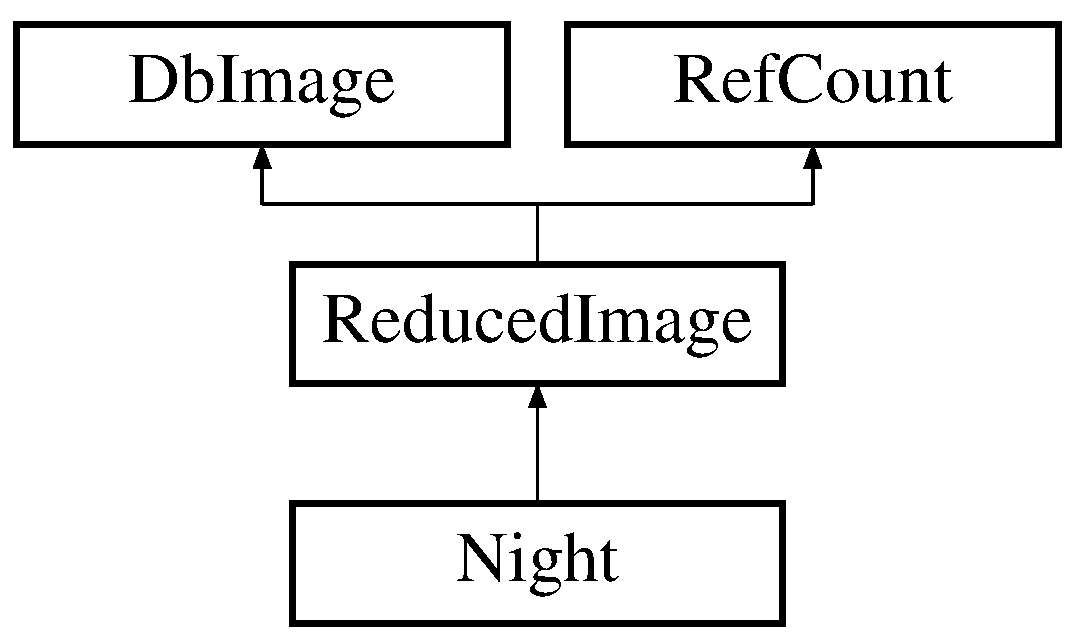
\includegraphics[height=3cm]{class_night}
\end{center}
\end{figure}
\subsubsection*{Public Methods}
\begin{CompactItemize}
\item 
\index{init@{init}!Night@{Night}}\index{Night@{Night}!init@{init}}
void {\bf init} ()\label{class_night_a0}

\begin{CompactList}\small\item\em Initialization of a night from its {\bf Reduced\-Image} {\rm (p.\,\pageref{class_reducedimage})}.\item\end{CompactList}\item 
\index{Night@{Night}!Night@{Night}}\index{Night@{Night}!Night@{Night}}
{\bf Night} (const string \&Name)\label{class_night_a1}

\item 
\index{Night@{Night}!Night@{Night}}\index{Night@{Night}!Night@{Night}}
{\bf Night} ()\label{class_night_a2}

\item 
\index{~Night@{$\sim$Night}!Night@{Night}}\index{Night@{Night}!~Night@{$\sim$Night}}
{\bf $\sim$Night} ()\label{class_night_a3}

\item 
\index{IsOK@{IsOK}!Night@{Night}}\index{Night@{Night}!IsOK@{Is\-OK}}
bool {\bf Is\-OK} () const\label{class_night_a4}

\begin{CompactList}\small\item\em returns true if the night verifies a bunch of criteria.\item\end{CompactList}\item 
\index{Clone@{Clone}!Night@{Night}}\index{Night@{Night}!Clone@{Clone}}
{\bf Reduced\-Image}$\ast$ {\bf Clone} () const\label{class_night_a5}

\begin{CompactList}\small\item\em copy constructor.\item\end{CompactList}\item 
\index{operator<@{operator$<$}!Night@{Night}}\index{Night@{Night}!operator<@{operator$<$}}
bool {\bf operator$<$} (const Night \&Right) const\label{class_night_a6}

\begin{CompactList}\small\item\em allows my\-Night1 $<$ my\-Night2 to sort in time.\item\end{CompactList}\item 
\index{dump@{dump}!Night@{Night}}\index{Night@{Night}!dump@{dump}}
void {\bf dump} (ostream \&Stream) const\label{class_night_a7}

\begin{CompactList}\small\item\em dumps basic info.\item\end{CompactList}\item 
\index{dump_header@{dump\_\-header}!Night@{Night}}\index{Night@{Night}!dump_header@{dump\_\-header}}
void {\bf dump\_\-header} (ostream \&Stream) const\label{class_night_a8}

\end{CompactItemize}
\subsubsection*{Public Attributes}
\begin{CompactItemize}
\item 
\index{saturation@{saturation}!Night@{Night}}\index{Night@{Night}!saturation@{saturation}}
double {\bf saturation}\label{class_night_m0}

\begin{CompactList}\small\item\em The saturation level.\item\end{CompactList}\item 
\index{photomRatio@{photomRatio}!Night@{Night}}\index{Night@{Night}!photomRatio@{photom\-Ratio}}
double {\bf photom\-Ratio}\label{class_night_m1}

\begin{CompactList}\small\item\em A photometric ratio with a given reference image.\item\end{CompactList}\item 
\index{kernelChi2@{kernelChi2}!Night@{Night}}\index{Night@{Night}!kernelChi2@{kernel\-Chi2}}
double {\bf kernel\-Chi2}\label{class_night_m2}

\begin{CompactList}\small\item\em A Chi2/Dof deriving from a kernel fitting procedure.\item\end{CompactList}\item 
\index{julianDate@{julianDate}!Night@{Night}}\index{Night@{Night}!julianDate@{julian\-Date}}
double {\bf julian\-Date}\label{class_night_m3}

\begin{CompactList}\small\item\em the julian date associated with the night.\item\end{CompactList}\item 
\index{exposure@{exposure}!Night@{Night}}\index{Night@{Night}!exposure@{exposure}}
double {\bf exposure}\label{class_night_m4}

\begin{CompactList}\small\item\em total exposure time for this night.\item\end{CompactList}\item 
\index{zeroPoint@{zeroPoint}!Night@{Night}}\index{Night@{Night}!zeroPoint@{zero\-Point}}
double {\bf zero\-Point}\label{class_night_m5}

\begin{CompactList}\small\item\em the zero point of the night.\item\end{CompactList}\item 
\index{seeing@{seeing}!Night@{Night}}\index{Night@{Night}!seeing@{seeing}}
double {\bf seeing}\label{class_night_m6}

\begin{CompactList}\small\item\em seeing (in pixel units) of the night.\item\end{CompactList}\item 
\index{sigmaX@{sigmaX}!Night@{Night}}\index{Night@{Night}!sigmaX@{sigma\-X}}
double {\bf sigma\-X}\label{class_night_m7}

\begin{CompactList}\small\item\em sigma (in pixel units) of the night PSF in x-direction.\item\end{CompactList}\item 
\index{sigmaY@{sigmaY}!Night@{Night}}\index{Night@{Night}!sigmaY@{sigma\-Y}}
double {\bf sigma\-Y}\label{class_night_m8}

\begin{CompactList}\small\item\em sigma (in pixel units) of the night PSF in y-direction.\item\end{CompactList}\item 
\index{thetaXY@{thetaXY}!Night@{Night}}\index{Night@{Night}!thetaXY@{theta\-XY}}
double {\bf theta\-XY}\label{class_night_m9}

\begin{CompactList}\small\item\em correlation angle of the night PSF.\item\end{CompactList}\item 
\index{skyLevel@{skyLevel}!Night@{Night}}\index{Night@{Night}!skyLevel@{sky\-Level}}
double {\bf sky\-Level}\label{class_night_m10}

\begin{CompactList}\small\item\em original sky background level of the night.\item\end{CompactList}\item 
\index{backLevel@{backLevel}!Night@{Night}}\index{Night@{Night}!backLevel@{back\-Level}}
double {\bf back\-Level}\label{class_night_m11}

\begin{CompactList}\small\item\em current background level of the image associated with the night.\item\end{CompactList}\item 
\index{sigmaSky@{sigmaSky}!Night@{Night}}\index{Night@{Night}!sigmaSky@{sigma\-Sky}}
double {\bf sigma\-Sky}\label{class_night_m12}

\begin{CompactList}\small\item\em sky RMS of the night sky background.\item\end{CompactList}\item 
\index{gain@{gain}!Night@{Night}}\index{Night@{Night}!gain@{gain}}
double {\bf gain}\label{class_night_m13}

\begin{CompactList}\small\item\em gain of the image (in e-/ADU).\item\end{CompactList}\item 
\index{flatError@{flatError}!Night@{Night}}\index{Night@{Night}!flatError@{flat\-Error}}
double {\bf flat\-Error}\label{class_night_m14}

\begin{CompactList}\small\item\em an estimate of the error in flatfielding (in \% of pixel intensity).\item\end{CompactList}\item 
\index{readoutNoise@{readoutNoise}!Night@{Night}}\index{Night@{Night}!readoutNoise@{readout\-Noise}}
double {\bf readout\-Noise}\label{class_night_m15}

\begin{CompactList}\small\item\em the readout noise in e-.\item\end{CompactList}\item 
\index{profileError@{profileError}!Night@{Night}}\index{Night@{Night}!profileError@{profile\-Error}}
double {\bf profile\-Error}\label{class_night_m16}

\begin{CompactList}\small\item\em the systematic error of the chosen PSF profile.\item\end{CompactList}\item 
\index{IsZeroRef@{IsZeroRef}!Night@{Night}}\index{Night@{Night}!IsZeroRef@{Is\-Zero\-Ref}}
bool {\bf Is\-Zero\-Ref}\label{class_night_m17}

\begin{CompactList}\small\item\em returns true if the night contribute as a zero point baseline for the lightcurve.\item\end{CompactList}\item 
\index{IsPhotometric@{IsPhotometric}!Night@{Night}}\index{Night@{Night}!IsPhotometric@{Is\-Photometric}}
bool {\bf Is\-Photometric}\label{class_night_m18}

\begin{CompactList}\small\item\em returns true if the night is photometric.\item\end{CompactList}\end{CompactItemize}
\subsubsection*{Friends}
\begin{CompactItemize}
\item 
class {\bf operator$<$$<$}
\end{CompactItemize}


\subsubsection{Detailed Description}
version of the {\bf Reduced\-Image} {\rm (p.\,\pageref{class_reducedimage})}, quicker, but with more memory.



The documentation for this class was generated from the following file:\begin{CompactItemize}
\item 
{\bf night.h}\end{CompactItemize}

\subsection{Night\-Element  Class Template Reference}
\label{class_nightelement}\index{NightElement@{Night\-Element}}
a template to use when an element belongs to a night. 


{\tt \#include $<$nightelement.h$>$}

Inheritance diagram for Night\-Element::\begin{figure}[H]
\begin{center}
\leavevmode
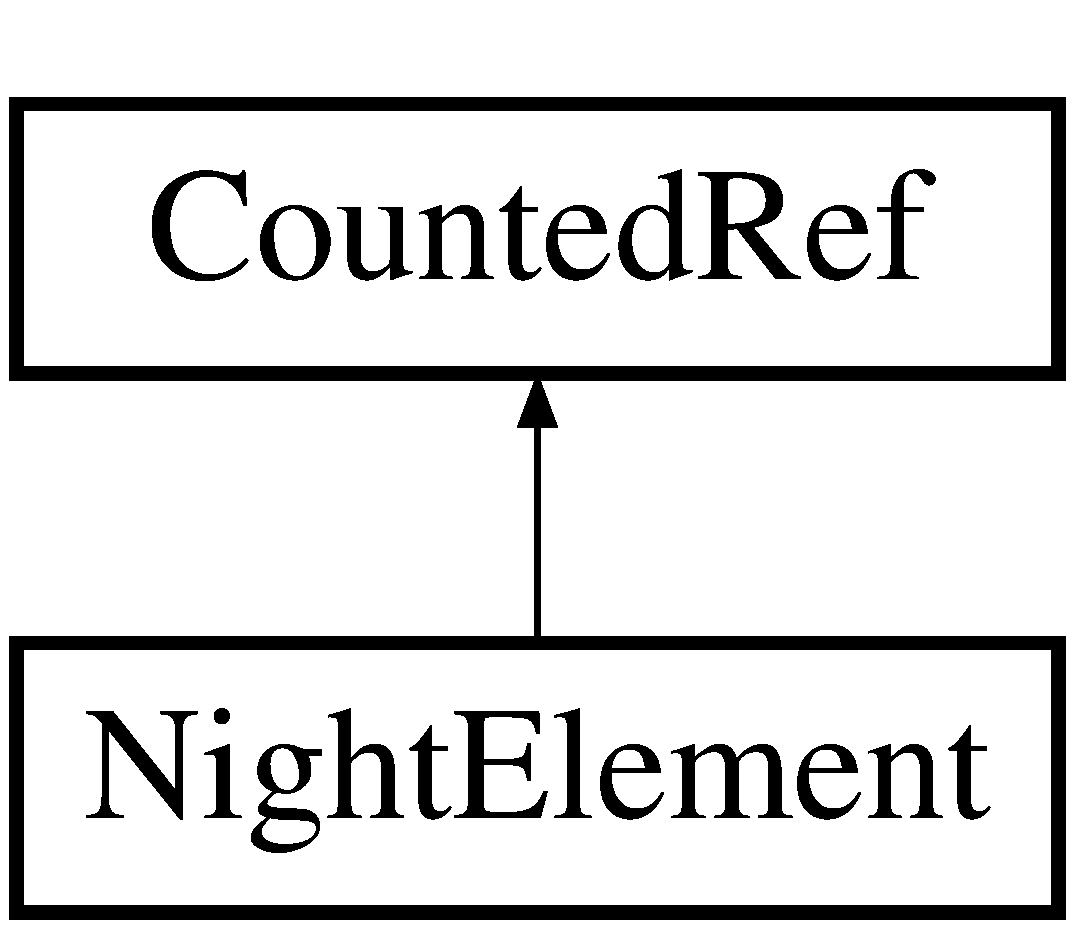
\includegraphics[height=2cm]{class_nightelement}
\end{center}
\end{figure}
\subsubsection*{Public Methods}
\begin{CompactItemize}
\item 
\index{NightElement@{NightElement}!NightElement@{Night\-Element}}\index{NightElement@{NightElement}!NightElement@{Night\-Element}}
{\bf Night\-Element} ()\label{class_nightelement_a0}

\begin{CompactList}\small\item\em empty constructor.\item\end{CompactList}\item 
\index{NightElement@{NightElement}!NightElement@{Night\-Element}}\index{NightElement@{NightElement}!NightElement@{Night\-Element}}
{\bf Night\-Element} (const Element \&An\-Element)\label{class_nightelement_a1}

\item 
\index{NightElement@{NightElement}!NightElement@{Night\-Element}}\index{NightElement@{NightElement}!NightElement@{Night\-Element}}
{\bf Night\-Element} (const {\bf Night} $\ast$ANight)\label{class_nightelement_a2}

\item 
\index{NightElement@{NightElement}!NightElement@{Night\-Element}}\index{NightElement@{NightElement}!NightElement@{Night\-Element}}
{\bf Night\-Element} (const Element \&An\-Element, const {\bf Night} $\ast$ANight)\label{class_nightelement_a3}

\item 
\index{~NightElement@{$\sim$NightElement}!NightElement@{Night\-Element}}\index{NightElement@{NightElement}!~NightElement@{$\sim$Night\-Element}}
{\bf $\sim$Night\-Element} ()\label{class_nightelement_a4}

\item 
\index{Clone@{Clone}!NightElement@{Night\-Element}}\index{NightElement@{NightElement}!Clone@{Clone}}
Night\-Element$\ast$ {\bf Clone} () const\label{class_nightelement_a5}

\end{CompactItemize}
\subsubsection*{Public Attributes}
\begin{CompactItemize}
\item 
\index{night@{night}!NightElement@{Night\-Element}}\index{NightElement@{NightElement}!night@{night}}
const {\bf Night}$\ast$ {\bf night}\label{class_nightelement_m0}

\end{CompactItemize}
\subsubsection*{Friends}
\begin{CompactItemize}
\item 
class {\bf By\-Increasing\-Seeing}
\item 
class {\bf By\-Increasing\-Time}
\end{CompactItemize}


\subsubsection{Detailed Description}
\subsubsection*{template$<$class Element$>$  class Night\-Element}

a template to use when an element belongs to a night.



The documentation for this class was generated from the following file:\begin{CompactItemize}
\item 
{\bf nightelement.h}\end{CompactItemize}

\subsection{Night\-Set  Class Reference}
\label{class_nightset}\index{NightSet@{Night\-Set}}
a class representing a set of overlapping images of the same night, same instrument and same filter. 


{\tt \#include $<$reducedutils.h$>$}

Inheritance diagram for Night\-Set::\begin{figure}[H]
\begin{center}
\leavevmode
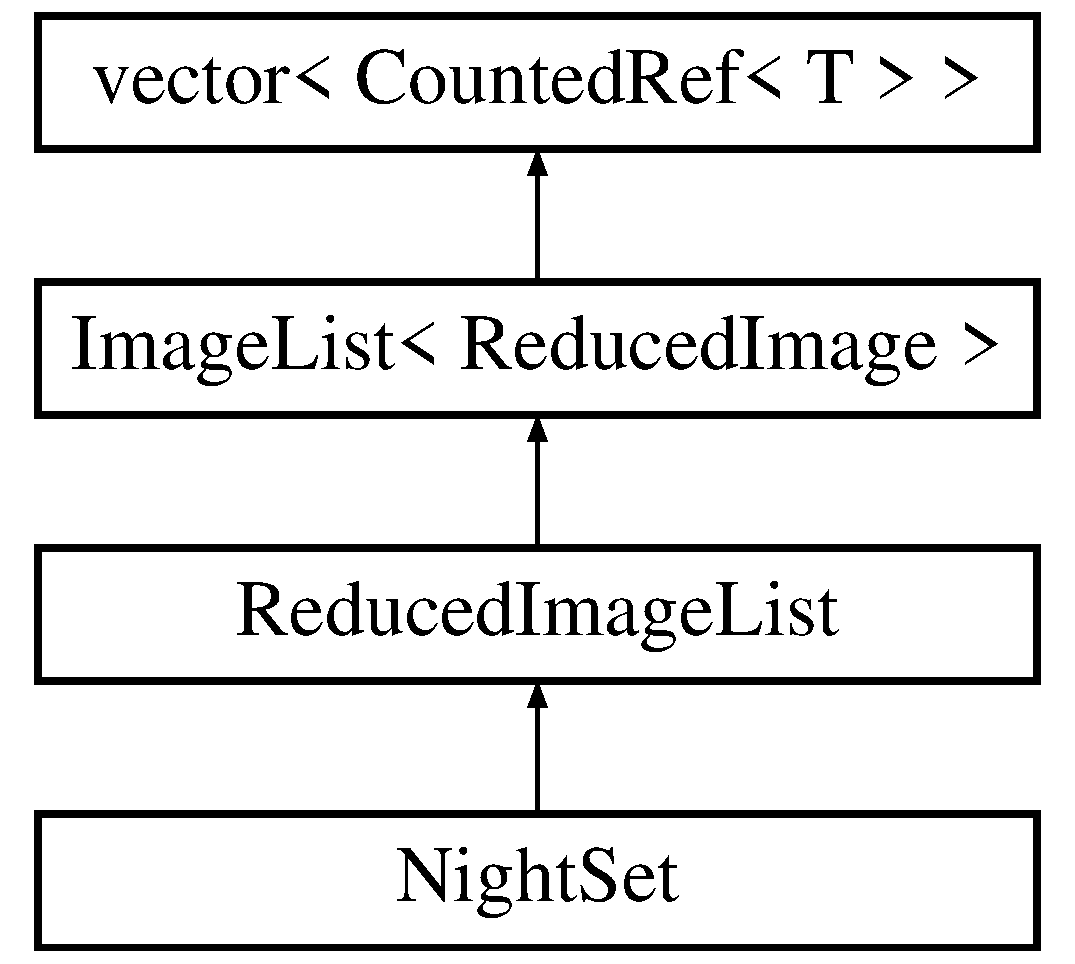
\includegraphics[height=4cm]{class_nightset}
\end{center}
\end{figure}
\subsubsection*{Public Methods}
\begin{CompactItemize}
\item 
\index{NightSet@{NightSet}!NightSet@{Night\-Set}}\index{NightSet@{NightSet}!NightSet@{Night\-Set}}
{\bf Night\-Set} (const {\bf Reduced\-Image} \&an\-Image)\label{class_nightset_a0}

\item 
\index{NightSet@{NightSet}!NightSet@{Night\-Set}}\index{NightSet@{NightSet}!NightSet@{Night\-Set}}
{\bf Night\-Set} (const Night\-Set \&Other)\label{class_nightset_a1}

\item 
\index{~NightSet@{$\sim$NightSet}!NightSet@{Night\-Set}}\index{NightSet@{NightSet}!~NightSet@{$\sim$Night\-Set}}
{\bf $\sim$Night\-Set} ()\label{class_nightset_a2}

\item 
\index{IsFromSameSet@{IsFromSameSet}!NightSet@{Night\-Set}}\index{NightSet@{NightSet}!IsFromSameSet@{Is\-From\-Same\-Set}}
bool {\bf Is\-From\-Same\-Set} (const {\bf Reduced\-Image} \&Another) const\label{class_nightset_a3}

\begin{CompactList}\small\item\em true if belongs to the same set.\item\end{CompactList}\item 
\index{GenericName@{GenericName}!NightSet@{Night\-Set}}\index{NightSet@{NightSet}!GenericName@{Generic\-Name}}
string {\bf Generic\-Name} () const\label{class_nightset_a4}

\begin{CompactList}\small\item\em returns the generic string name of the set.\item\end{CompactList}\item 
\index{dump@{dump}!NightSet@{Night\-Set}}\index{NightSet@{NightSet}!dump@{dump}}
void {\bf dump} (ostream \&Stream=cout) const\label{class_nightset_a5}

\item 
\index{Seeing@{Seeing}!NightSet@{Night\-Set}}\index{NightSet@{NightSet}!Seeing@{Seeing}}
double {\bf Seeing} () const\label{class_nightset_a6}

\item 
\index{Exposure@{Exposure}!NightSet@{Night\-Set}}\index{NightSet@{NightSet}!Exposure@{Exposure}}
double {\bf Exposure} () const\label{class_nightset_a7}

\item 
\index{SignalToNoise23@{SignalToNoise23}!NightSet@{Night\-Set}}\index{NightSet@{NightSet}!SignalToNoise23@{Signal\-To\-Noise23}}
double {\bf Signal\-To\-Noise23} () const\label{class_nightset_a8}

\end{CompactItemize}
\subsubsection*{Friends}
\begin{CompactItemize}
\item 
\index{operator<<@{operator$<$$<$}!NightSet@{Night\-Set}}\index{NightSet@{NightSet}!operator<<@{operator$<$$<$}}
ostream\& {\bf operator$<$$<$} (ostream \&Stream, const Night\-Set \&My\-Set)\label{class_nightset_l0}

\begin{CompactList}\small\item\em allows cout $<$$<$ Nigh\-Set;.\item\end{CompactList}\end{CompactItemize}


\subsubsection{Detailed Description}
a class representing a set of overlapping images of the same night, same instrument and same filter.



The documentation for this class was generated from the following file:\begin{CompactItemize}
\item 
{\bf reducedutils.h}\end{CompactItemize}

\subsection{Point  Class Reference}
\label{class_point}\index{Point@{Point}}
A point in a plane. 


{\tt \#include $<$point.h$>$}

Inheritance diagram for Point::\begin{figure}[H]
\begin{center}
\leavevmode
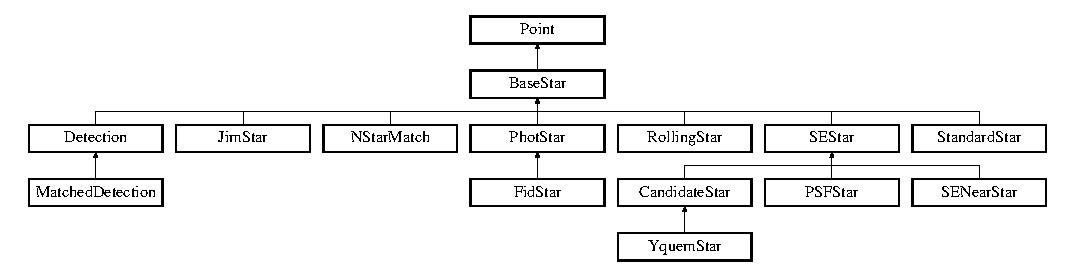
\includegraphics[height=3.27869cm]{class_point}
\end{center}
\end{figure}
\subsubsection*{Public Methods}
\begin{CompactItemize}
\item 
\index{Point@{Point}!Point@{Point}}\index{Point@{Point}!Point@{Point}}
{\bf Point} (const double \&xx=0, const double \&yy=0)\label{class_point_a0}

\begin{CompactList}\small\item\em \begin{CompactItemize}
\item 
contructor.\end{CompactItemize}
\item\end{CompactList}\item 
\index{Distance@{Distance}!Point@{Point}}\index{Point@{Point}!Distance@{Distance}}
double {\bf Distance} (const Point \&Other) const\label{class_point_a1}

\begin{CompactList}\small\item\em -.\item\end{CompactList}\item 
\index{Dist2@{Dist2}!Point@{Point}}\index{Point@{Point}!Dist2@{Dist2}}
double {\bf Dist2} (const Point \&Other) const\label{class_point_a2}

\begin{CompactList}\small\item\em distance squared to Other.\item\end{CompactList}\item 
\index{Apply@{Apply}!Point@{Point}}\index{Point@{Point}!Apply@{Apply}}
template$<$class Operator$>$ void {\bf Apply} (const Operator \&Op)\label{class_point_a3}

\begin{CompactList}\small\item\em Operator can be e.g. a {\bf Gtransfo} {\rm (p.\,\pageref{class_gtransfo})}.\item\end{CompactList}\item 
\index{operator+@{operator+}!Point@{Point}}\index{Point@{Point}!operator+@{operator+}}
Point {\bf operator+} (const Point \&Right) const\label{class_point_a4}

\begin{CompactList}\small\item\em Sum.\item\end{CompactList}\item 
\index{operator-@{operator-}!Point@{Point}}\index{Point@{Point}!operator-@{operator-}}
Point {\bf operator-} (const Point \&Right) const\label{class_point_a5}

\begin{CompactList}\small\item\em Difference.\item\end{CompactList}\item 
\index{dump@{dump}!Point@{Point}}\index{Point@{Point}!dump@{dump}}
virtual void {\bf dump} (ostream \&s=cout) const\label{class_point_a6}

\end{CompactItemize}
\subsubsection*{Public Attributes}
\begin{CompactItemize}
\item 
\index{x@{x}!Point@{Point}}\index{Point@{Point}!x@{x}}
double {\bf x}\label{class_point_m0}

\begin{CompactList}\small\item\em coordinate.\item\end{CompactList}\item 
\index{y@{y}!Point@{Point}}\index{Point@{Point}!y@{y}}
double {\bf y}\label{class_point_m1}

\begin{CompactList}\small\item\em coordinate.\item\end{CompactList}\end{CompactItemize}
\subsubsection*{Friends}
\begin{CompactItemize}
\item 
\index{operator<<@{operator$<$$<$}!Point@{Point}}\index{Point@{Point}!operator<<@{operator$<$$<$}}
ostream\& {\bf operator$<$$<$} (ostream \&stream, const Point \&point)\label{class_point_l0}

\begin{CompactList}\small\item\em -.\item\end{CompactList}\end{CompactItemize}


\subsubsection{Detailed Description}
A point in a plane.



The documentation for this class was generated from the following file:\begin{CompactItemize}
\item 
{\bf point.h}\end{CompactItemize}

\subsection{Psf\-Match  Class Reference}
\label{class_psfmatch}\index{PsfMatch@{Psf\-Match}}
A class that wraps calls to {\bf Kernel\-Fit} {\rm (p.\,\pageref{class_kernelfit})}. Used both to carry out subtractions ({\bf Image\-Subtraction} {\rm (p.\,\pageref{class_imagesubtraction})}) and just kernel fitting (for the light curve). 


{\tt \#include $<$psfmatch.h$>$}

Inheritance diagram for Psf\-Match::\begin{figure}[H]
\begin{center}
\leavevmode
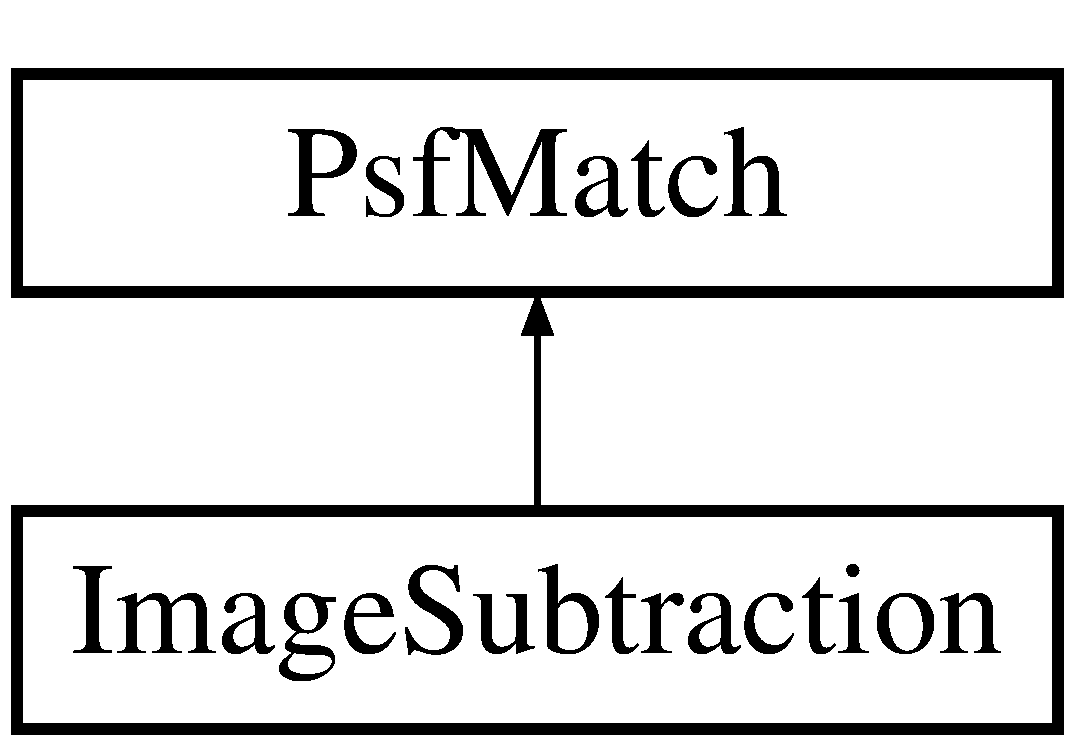
\includegraphics[height=2cm]{class_psfmatch}
\end{center}
\end{figure}
\subsubsection*{Public Methods}
\begin{CompactItemize}
\item 
\index{NotFilteredStarListName@{NotFilteredStarListName}!PsfMatch@{Psf\-Match}}\index{PsfMatch@{PsfMatch}!NotFilteredStarListName@{Not\-Filtered\-Star\-List\-Name}}
string {\bf Not\-Filtered\-Star\-List\-Name} ()\label{class_psfmatch_a0}

\item 
\index{PsfMatch@{PsfMatch}!PsfMatch@{Psf\-Match}}\index{PsfMatch@{PsfMatch}!PsfMatch@{Psf\-Match}}
{\bf Psf\-Match} (const {\bf Reduced\-Image} \&Ref, const {\bf Reduced\-Image} \&New, const Psf\-Match $\ast$APrevious\-Match=NULL)\label{class_psfmatch_a1}

\item 
\index{~PsfMatch@{$\sim$PsfMatch}!PsfMatch@{Psf\-Match}}\index{PsfMatch@{PsfMatch}!~PsfMatch@{$\sim$Psf\-Match}}
{\bf $\sim$Psf\-Match} ()\label{class_psfmatch_a2}

\item 
\index{PsfMatch@{PsfMatch}!PsfMatch@{Psf\-Match}}\index{PsfMatch@{PsfMatch}!PsfMatch@{Psf\-Match}}
{\bf Psf\-Match} (const Psf\-Match \&Original)\label{class_psfmatch_a3}

\item 
\index{PsfMatch@{PsfMatch}!PsfMatch@{Psf\-Match}}\index{PsfMatch@{PsfMatch}!PsfMatch@{Psf\-Match}}
{\bf Psf\-Match} ()\label{class_psfmatch_a4}

\item 
\index{FitKernel@{FitKernel}!PsfMatch@{Psf\-Match}}\index{PsfMatch@{PsfMatch}!FitKernel@{Fit\-Kernel}}
bool {\bf Fit\-Kernel} (const bool Keep\-Images=false)\label{class_psfmatch_a5}

\begin{CompactList}\small\item\em Carry out kernel fit. argument to enable to keep the images.\item\end{CompactList}\item 
\index{FilterStarList@{FilterStarList}!PsfMatch@{Psf\-Match}}\index{PsfMatch@{PsfMatch}!FilterStarList@{Filter\-Star\-List}}
int {\bf Filter\-Star\-List} (const double Max\-Dist=1)\label{class_psfmatch_a6}

\item 
\index{PhotomRatio@{PhotomRatio}!PsfMatch@{Psf\-Match}}\index{PsfMatch@{PsfMatch}!PhotomRatio@{Photom\-Ratio}}
double {\bf Photom\-Ratio} () const\label{class_psfmatch_a7}

\item 
\index{Chi2@{Chi2}!PsfMatch@{Psf\-Match}}\index{PsfMatch@{PsfMatch}!Chi2@{Chi2}}
double {\bf Chi2} () const\label{class_psfmatch_a8}

\item 
\index{SigmaBack@{SigmaBack}!PsfMatch@{Psf\-Match}}\index{PsfMatch@{PsfMatch}!SigmaBack@{Sigma\-Back}}
double {\bf Sigma\-Back} () const\label{class_psfmatch_a9}

\item 
\index{Intersection@{Intersection}!PsfMatch@{Psf\-Match}}\index{PsfMatch@{PsfMatch}!Intersection@{Intersection}}
{\bf Frame} {\bf Intersection} () const\label{class_psfmatch_a10}

\item 
\index{KernelToWorst@{KernelToWorst}!PsfMatch@{Psf\-Match}}\index{PsfMatch@{PsfMatch}!KernelToWorst@{Kernel\-To\-Worst}}
void {\bf Kernel\-To\-Worst} ({\bf Kernel} \&Result, const double \&x, const double \&y) const\label{class_psfmatch_a11}

\item 
\index{BackKernel@{BackKernel}!PsfMatch@{Psf\-Match}}\index{PsfMatch@{PsfMatch}!BackKernel@{Back\-Kernel}}
void {\bf Back\-Kernel} ({\bf Kernel} \&Diffback, const double \&xc, const double \&yc)\label{class_psfmatch_a12}

\item 
\index{VarianceConvolve@{VarianceConvolve}!PsfMatch@{Psf\-Match}}\index{PsfMatch@{PsfMatch}!VarianceConvolve@{Variance\-Convolve}}
bool {\bf Variance\-Convolve} ({\bf Image} \&Variance)\label{class_psfmatch_a13}

\begin{CompactList}\small\item\em builds the subtraction image new-ref (in photometric units of the ref). Puts it as the fits image of RImage. Sets seeing \& co. Does not keep by default the result of the convolution.\item\end{CompactList}\item 
\index{ConvolveBest@{ConvolveBest}!PsfMatch@{Psf\-Match}}\index{PsfMatch@{PsfMatch}!ConvolveBest@{Convolve\-Best}}
void {\bf Convolve\-Best} ({\bf Reduced\-Image} \&Conv\-Image)\label{class_psfmatch_a14}

\item 
\index{Subtraction@{Subtraction}!PsfMatch@{Psf\-Match}}\index{PsfMatch@{PsfMatch}!Subtraction@{Subtraction}}
bool {\bf Subtraction} ({\bf Reduced\-Image} \&RImage, bool Keep\-Convolved\-Best=false)\label{class_psfmatch_a15}

\item 
\index{RefIsBest@{RefIsBest}!PsfMatch@{Psf\-Match}}\index{PsfMatch@{PsfMatch}!RefIsBest@{Ref\-Is\-Best}}
bool {\bf Ref\-Is\-Best} () const\label{class_psfmatch_a16}

\item 
\index{Ref@{Ref}!PsfMatch@{Psf\-Match}}\index{PsfMatch@{PsfMatch}!Ref@{Ref}}
{\bf Reduced\-Image}$\ast$ {\bf Ref} ()\label{class_psfmatch_a17}

\item 
\index{New@{New}!PsfMatch@{Psf\-Match}}\index{PsfMatch@{PsfMatch}!New@{New}}
{\bf Reduced\-Image}$\ast$ {\bf New} ()\label{class_psfmatch_a18}

\item 
\index{Best@{Best}!PsfMatch@{Psf\-Match}}\index{PsfMatch@{PsfMatch}!Best@{Best}}
{\bf Reduced\-Image}$\ast$ {\bf Best} ()\label{class_psfmatch_a19}

\item 
\index{Worst@{Worst}!PsfMatch@{Psf\-Match}}\index{PsfMatch@{PsfMatch}!Worst@{Worst}}
{\bf Reduced\-Image}$\ast$ {\bf Worst} ()\label{class_psfmatch_a20}

\end{CompactItemize}
\subsubsection*{Public Attributes}
\begin{CompactItemize}
\item 
\index{objectsUsedToFit@{objectsUsedToFit}!PsfMatch@{Psf\-Match}}\index{PsfMatch@{PsfMatch}!objectsUsedToFit@{objects\-Used\-To\-Fit}}
Base\-Star\-List {\bf objects\-Used\-To\-Fit}\label{class_psfmatch_m0}

\end{CompactItemize}


\subsubsection{Detailed Description}
A class that wraps calls to {\bf Kernel\-Fit} {\rm (p.\,\pageref{class_kernelfit})}. Used both to carry out subtractions ({\bf Image\-Subtraction} {\rm (p.\,\pageref{class_imagesubtraction})}) and just kernel fitting (for the light curve).



The documentation for this class was generated from the following files:\begin{CompactItemize}
\item 
{\bf psfmatch.h}\item 
psfmatch.cc\end{CompactItemize}

\subsection{Psf\-Stars  Class Reference}
\label{class_psfstars}\index{PsfStars@{Psf\-Stars}}
a class to select PSF stars from different ways. 


{\tt \#include $<$daophotpsf.h$>$}

Inheritance diagram for Psf\-Stars::\begin{figure}[H]
\begin{center}
\leavevmode
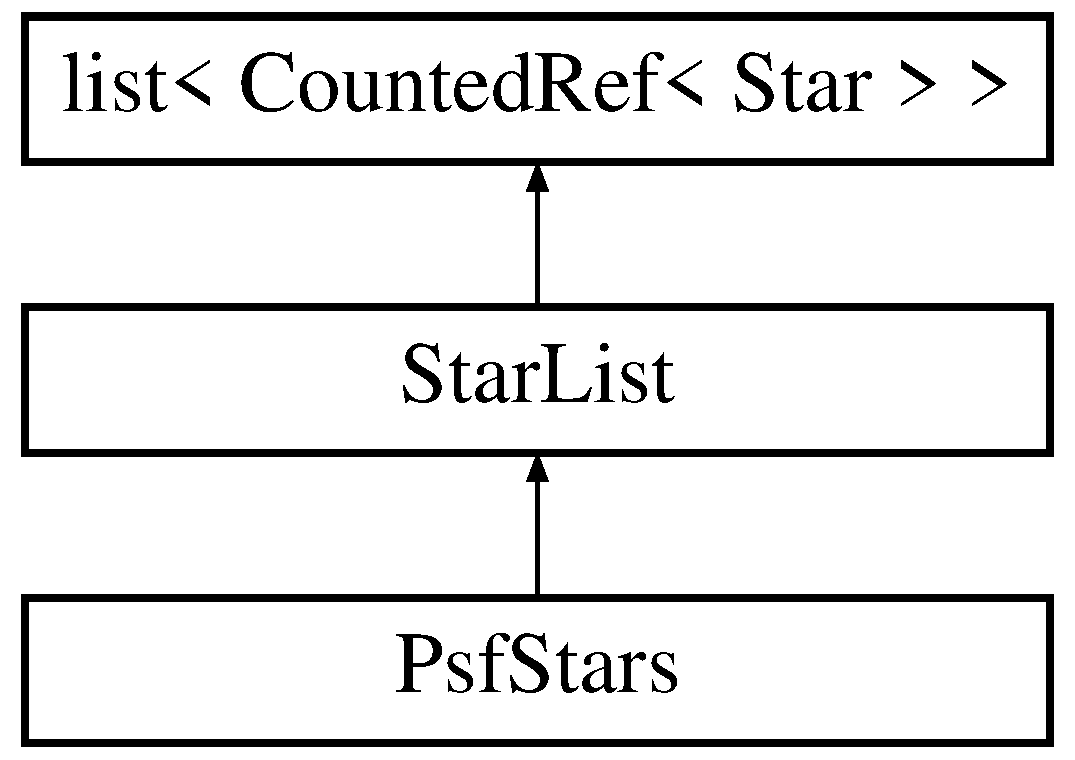
\includegraphics[height=3cm]{class_psfstars}
\end{center}
\end{figure}
\subsubsection*{Public Methods}
\begin{CompactItemize}
\item 
\index{PsfStars@{PsfStars}!PsfStars@{Psf\-Stars}}\index{PsfStars@{PsfStars}!PsfStars@{Psf\-Stars}}
{\bf Psf\-Stars} (const {\bf Reduced\-Image} \&Rim)\label{class_psfstars_a0}

\begin{CompactList}\small\item\em just reads in the decent objects from a {\bf Reduced\-Image} {\rm (p.\,\pageref{class_reducedimage})}.\item\end{CompactList}\item 
\index{~PsfStars@{$\sim$PsfStars}!PsfStars@{Psf\-Stars}}\index{PsfStars@{PsfStars}!~PsfStars@{$\sim$Psf\-Stars}}
{\bf $\sim$Psf\-Stars} ()\label{class_psfstars_a1}

\item 
\index{FilterNei@{FilterNei}!PsfStars@{Psf\-Stars}}\index{PsfStars@{PsfStars}!FilterNei@{Filter\-Nei}}
size\_\-t {\bf Filter\-Nei} ()\label{class_psfstars_a2}

\begin{CompactList}\small\item\em removes the stars with bad flags on the neighbor file created during PSF building.\item\end{CompactList}\item 
\index{FilterAls@{FilterAls}!PsfStars@{Psf\-Stars}}\index{PsfStars@{PsfStars}!FilterAls@{Filter\-Als}}
size\_\-t {\bf Filter\-Als} (const double Chi\-Max=3.0, const double Sharp\-Min=-0.5, const double Sharp\-Max=0.5)\label{class_psfstars_a3}

\begin{CompactList}\small\item\em removes the stars from the file created by ALLSTAR, given some cuts.\item\end{CompactList}\item 
\index{FilterCond@{FilterCond}!PsfStars@{Psf\-Stars}}\index{PsfStars@{PsfStars}!FilterCond@{Filter\-Cond}}
size\_\-t {\bf Filter\-Cond} (const Psf\-Conditions \&Cond)\label{class_psfstars_a4}

\begin{CompactList}\small\item\em removes the stars which do not verify the conditions Cond.\item\end{CompactList}\item 
\index{FilterMultiIm@{FilterMultiIm}!PsfStars@{Psf\-Stars}}\index{PsfStars@{PsfStars}!FilterMultiIm@{Filter\-Multi\-Im}}
size\_\-t {\bf Filter\-Multi\-Im} (const Reduced\-Image\-List \&Rim\-List, const {\bf Reduced\-Image} $\ast$ref, const double Max\-Dist=2)\label{class_psfstars_a5}

\begin{CompactList}\small\item\em keeps the stars in the set of images in Rim\-List.\item\end{CompactList}\end{CompactItemize}


\subsubsection{Detailed Description}
a class to select PSF stars from different ways.



The documentation for this class was generated from the following file:\begin{CompactItemize}
\item 
{\bf daophotpsf.h}\end{CompactItemize}

\subsection{Reduced\-Image  Class Reference}
\label{class_reducedimage}\index{ReducedImage@{Reduced\-Image}}
a handle to access data associated to an image: the fits file, the catalog, the dead and satur frames, and a set of 'scalars' such as seeing, saturation level \&co. 


{\tt \#include $<$reducedimage.h$>$}

Inheritance diagram for Reduced\-Image::\begin{figure}[H]
\begin{center}
\leavevmode
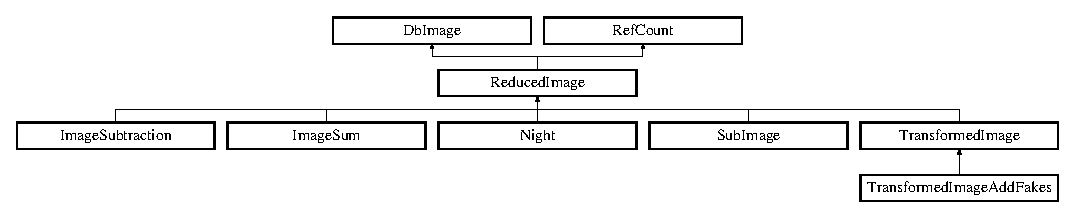
\includegraphics[height=2.47514cm]{class_reducedimage}
\end{center}
\end{figure}
\subsubsection*{Public Methods}
\begin{CompactItemize}
\item 
\index{ReducedImage@{ReducedImage}!ReducedImage@{Reduced\-Image}}\index{ReducedImage@{ReducedImage}!ReducedImage@{Reduced\-Image}}
{\bf Reduced\-Image} ()\label{class_reducedimage_a0}

\item 
\index{ReducedImage@{ReducedImage}!ReducedImage@{Reduced\-Image}}\index{ReducedImage@{ReducedImage}!ReducedImage@{Reduced\-Image}}
{\bf Reduced\-Image} (const {\bf Db\-Image} \&)\label{class_reducedimage_a1}

\item 
\index{ReducedImage@{ReducedImage}!ReducedImage@{Reduced\-Image}}\index{ReducedImage@{ReducedImage}!ReducedImage@{Reduced\-Image}}
{\bf Reduced\-Image} (const string \&Name)\label{class_reducedimage_a2}

\item 
\index{HasImage@{HasImage}!ReducedImage@{Reduced\-Image}}\index{ReducedImage@{ReducedImage}!HasImage@{Has\-Image}}
bool {\bf Has\-Image} () const\label{class_reducedimage_a3}

\item 
\index{HasBack@{HasBack}!ReducedImage@{Reduced\-Image}}\index{ReducedImage@{ReducedImage}!HasBack@{Has\-Back}}
bool {\bf Has\-Back} () const\label{class_reducedimage_a4}

\item 
\index{HasMiniBack@{HasMiniBack}!ReducedImage@{Reduced\-Image}}\index{ReducedImage@{ReducedImage}!HasMiniBack@{Has\-Mini\-Back}}
bool {\bf Has\-Mini\-Back} () const\label{class_reducedimage_a5}

\item 
\index{HasCatalog@{HasCatalog}!ReducedImage@{Reduced\-Image}}\index{ReducedImage@{ReducedImage}!HasCatalog@{Has\-Catalog}}
bool {\bf Has\-Catalog} () const\label{class_reducedimage_a6}

\item 
\index{HasDead@{HasDead}!ReducedImage@{Reduced\-Image}}\index{ReducedImage@{ReducedImage}!HasDead@{Has\-Dead}}
bool {\bf Has\-Dead} () const\label{class_reducedimage_a7}

\item 
\index{HasFlat@{HasFlat}!ReducedImage@{Reduced\-Image}}\index{ReducedImage@{ReducedImage}!HasFlat@{Has\-Flat}}
bool {\bf Has\-Flat} () const\label{class_reducedimage_a8}

\item 
\index{HasSatur@{HasSatur}!ReducedImage@{Reduced\-Image}}\index{ReducedImage@{ReducedImage}!HasSatur@{Has\-Satur}}
bool {\bf Has\-Satur} () const\label{class_reducedimage_a9}

\item 
\index{HasCosmic@{HasCosmic}!ReducedImage@{Reduced\-Image}}\index{ReducedImage@{ReducedImage}!HasCosmic@{Has\-Cosmic}}
bool {\bf Has\-Cosmic} () const\label{class_reducedimage_a10}

\item 
\index{HasSatellite@{HasSatellite}!ReducedImage@{Reduced\-Image}}\index{ReducedImage@{ReducedImage}!HasSatellite@{Has\-Satellite}}
bool {\bf Has\-Satellite} () const\label{class_reducedimage_a11}

\item 
\index{HasWeight@{HasWeight}!ReducedImage@{Reduced\-Image}}\index{ReducedImage@{ReducedImage}!HasWeight@{Has\-Weight}}
bool {\bf Has\-Weight} () const\label{class_reducedimage_a12}

\item 
\index{HasBad@{HasBad}!ReducedImage@{Reduced\-Image}}\index{ReducedImage@{ReducedImage}!HasBad@{Has\-Bad}}
bool {\bf Has\-Bad} () const\label{class_reducedimage_a13}

\item 
\index{FitsName@{FitsName}!ReducedImage@{Reduced\-Image}}\index{ReducedImage@{ReducedImage}!FitsName@{Fits\-Name}}
string {\bf Fits\-Name} () const\label{class_reducedimage_a14}

\begin{CompactList}\small\item\em not const because it may actually compute the image and other things (for derived class).\item\end{CompactList}\item 
\index{MakeFits@{MakeFits}!ReducedImage@{Reduced\-Image}}\index{ReducedImage@{ReducedImage}!MakeFits@{Make\-Fits}}
virtual bool {\bf Make\-Fits} ()\label{class_reducedimage_a15}

\begin{CompactList}\small\item\em produce fits image.\item\end{CompactList}\item 
\index{CatalogName@{CatalogName}!ReducedImage@{Reduced\-Image}}\index{ReducedImage@{ReducedImage}!CatalogName@{Catalog\-Name}}
string {\bf Catalog\-Name} () const\label{class_reducedimage_a16}

\item 
\index{FillSExtractorData@{FillSExtractorData}!ReducedImage@{Reduced\-Image}}\index{ReducedImage@{ReducedImage}!FillSExtractorData@{Fill\-SExtractor\-Data}}
void {\bf Fill\-SExtractor\-Data} (For\-SExtractor \&data, bool fond\_\-deja\_\-soustrait, bool sauver\_\-fond, bool use\_\-sigma\_\-header)\label{class_reducedimage_a17}

\item 
\index{RecoverBack@{RecoverBack}!ReducedImage@{Reduced\-Image}}\index{ReducedImage@{ReducedImage}!RecoverBack@{Recover\-Back}}
bool {\bf Recover\-Back} (bool add\_\-to\_\-im)\label{class_reducedimage_a18}

\item 
\index{ReAddBackground_and_ResetKeys@{ReAddBackground\_\-and\_\-ResetKeys}!ReducedImage@{Reduced\-Image}}\index{ReducedImage@{ReducedImage}!ReAddBackground_and_ResetKeys@{Re\-Add\-Background\_\-and\_\-Reset\-Keys}}
bool {\bf Re\-Add\-Background\_\-and\_\-Reset\-Keys} ()\label{class_reducedimage_a19}

\item 
\index{MakeCatalog@{MakeCatalog}!ReducedImage@{Reduced\-Image}}\index{ReducedImage@{ReducedImage}!MakeCatalog@{Make\-Catalog}}
bool {\bf Make\-Catalog} (bool redo\_\-from\_\-beg, bool overwrite, bool savemasksat, bool pas\_\-sub\_\-fond, bool use\_\-sigma\_\-header)\label{class_reducedimage_a20}

\item 
\index{MakeCatalog@{MakeCatalog}!ReducedImage@{Reduced\-Image}}\index{ReducedImage@{ReducedImage}!MakeCatalog@{Make\-Catalog}}
virtual bool {\bf Make\-Catalog} ()\label{class_reducedimage_a21}

\begin{CompactList}\small\item\em Produce the Saturated stars pixels mask, subtract the image background, detect with the SExtractor computed sigma. search the cosmics, and update catalog and weight for cosmics. No free coffee.\item\end{CompactList}\item 
\index{MakeCatalog_ImageBizarre@{MakeCatalog\_\-ImageBizarre}!ReducedImage@{Reduced\-Image}}\index{ReducedImage@{ReducedImage}!MakeCatalog_ImageBizarre@{Make\-Catalog\_\-Image\-Bizarre}}
bool {\bf Make\-Catalog\_\-Image\-Bizarre} ()\label{class_reducedimage_a22}

\begin{CompactList}\small\item\em {\bf Make\-Catalog\_\-Image\-Bizarre}() {\rm (p.\,\pageref{class_reducedimage_a22})} is for sum-images, or convolved images, for which we do not want to subtract the background map, nor computing the saturated pixels map, and for which we provide the value of the sigmabackground. overwrite is set to true.\item\end{CompactList}\item 
\index{MakeSatur@{MakeSatur}!ReducedImage@{Reduced\-Image}}\index{ReducedImage@{ReducedImage}!MakeSatur@{Make\-Satur}}
virtual bool {\bf Make\-Satur} ()\label{class_reducedimage_a23}

\begin{CompactList}\small\item\em produce satur image.\item\end{CompactList}\item 
\index{MakeDead@{MakeDead}!ReducedImage@{Reduced\-Image}}\index{ReducedImage@{ReducedImage}!MakeDead@{Make\-Dead}}
virtual bool {\bf Make\-Dead} ()\label{class_reducedimage_a24}

\begin{CompactList}\small\item\em produce dead image.\item\end{CompactList}\item 
\index{FlagCosmicsInCatalog@{FlagCosmicsInCatalog}!ReducedImage@{Reduced\-Image}}\index{ReducedImage@{ReducedImage}!FlagCosmicsInCatalog@{Flag\-Cosmics\-In\-Catalog}}
void {\bf Flag\-Cosmics\-In\-Catalog} (const {\bf Image} \&Cosmic\-Image, const double dist=2)\label{class_reducedimage_a25}

\item 
\index{MakeCosmic@{MakeCosmic}!ReducedImage@{Reduced\-Image}}\index{ReducedImage@{ReducedImage}!MakeCosmic@{Make\-Cosmic}}
virtual bool {\bf Make\-Cosmic} ()\label{class_reducedimage_a26}

\begin{CompactList}\small\item\em produce cosmic image.\item\end{CompactList}\item 
\index{MakeSatellite@{MakeSatellite}!ReducedImage@{Reduced\-Image}}\index{ReducedImage@{ReducedImage}!MakeSatellite@{Make\-Satellite}}
virtual bool {\bf Make\-Satellite} ()\label{class_reducedimage_a27}

\begin{CompactList}\small\item\em produce satellite image.\item\end{CompactList}\item 
\index{IsToadsWeight@{IsToadsWeight}!ReducedImage@{Reduced\-Image}}\index{ReducedImage@{ReducedImage}!IsToadsWeight@{Is\-Toads\-Weight}}
bool {\bf Is\-Toads\-Weight} ()\label{class_reducedimage_a28}

\begin{CompactList}\small\item\em produce weight image.\item\end{CompactList}\item 
\index{MakeWeight@{MakeWeight}!ReducedImage@{Reduced\-Image}}\index{ReducedImage@{ReducedImage}!MakeWeight@{Make\-Weight}}
virtual bool {\bf Make\-Weight} ()\label{class_reducedimage_a29}

\item 
\index{MakeBad@{MakeBad}!ReducedImage@{Reduced\-Image}}\index{ReducedImage@{ReducedImage}!MakeBad@{Make\-Bad}}
virtual bool {\bf Make\-Bad} ()\label{class_reducedimage_a30}

\begin{CompactList}\small\item\em produce bad pixel image.\item\end{CompactList}\item 
\index{ActuallyReduced@{ActuallyReduced}!ReducedImage@{Reduced\-Image}}\index{ReducedImage@{ReducedImage}!ActuallyReduced@{Actually\-Reduced}}
bool {\bf Actually\-Reduced} () const\label{class_reducedimage_a31}

\begin{CompactList}\small\item\em returns if both fits image and catalog file exist.\item\end{CompactList}\item 
\index{Execute@{Execute}!ReducedImage@{Reduced\-Image}}\index{ReducedImage@{ReducedImage}!Execute@{Execute}}
bool {\bf Execute} (const int To\-Do)\label{class_reducedimage_a32}

\begin{CompactList}\small\item\em shorthand call for Make\{Fits,Catalog,Dead,Satur\}. To\-Do may conveniently be contructed using predefined tags Do\-Fits Do\-Catalog Do\-Dead Do\-Satur.\item\end{CompactList}\item 
\index{TypeName@{TypeName}!ReducedImage@{Reduced\-Image}}\index{ReducedImage@{ReducedImage}!TypeName@{Type\-Name}}
string {\bf Type\-Name} () const\label{class_reducedimage_a33}

\item 
\index{SetTypeName@{SetTypeName}!ReducedImage@{Reduced\-Image}}\index{ReducedImage@{ReducedImage}!SetTypeName@{Set\-Type\-Name}}
bool {\bf Set\-Type\-Name} (const string \&Type\-Name)\label{class_reducedimage_a34}

\item 
\index{TypeFileName@{TypeFileName}!ReducedImage@{Reduced\-Image}}\index{ReducedImage@{ReducedImage}!TypeFileName@{Type\-File\-Name}}
string {\bf Type\-File\-Name} () const\label{class_reducedimage_a35}

\item 
\index{dump@{dump}!ReducedImage@{Reduced\-Image}}\index{ReducedImage@{ReducedImage}!dump@{dump}}
virtual void {\bf dump} (ostream \&s=cout) const\label{class_reducedimage_a36}

\begin{CompactList}\small\item\em dumps basic info.\item\end{CompactList}\item 
\index{XSize@{XSize}!ReducedImage@{Reduced\-Image}}\index{ReducedImage@{ReducedImage}!XSize@{XSize}}
int {\bf XSize} () const\label{class_reducedimage_a37}

\begin{CompactList}\small\item\em size in x-axis.\item\end{CompactList}\item 
\index{YSize@{YSize}!ReducedImage@{Reduced\-Image}}\index{ReducedImage@{ReducedImage}!YSize@{YSize}}
int {\bf YSize} () const\label{class_reducedimage_a38}

\begin{CompactList}\small\item\em size in y-axis.\item\end{CompactList}\item 
\index{Seeing@{Seeing}!ReducedImage@{Reduced\-Image}}\index{ReducedImage@{ReducedImage}!Seeing@{Seeing}}
double {\bf Seeing} () const\label{class_reducedimage_a39}

\begin{CompactList}\small\item\em basic seeing.\item\end{CompactList}\item 
\index{RemoveSeeing@{RemoveSeeing}!ReducedImage@{Reduced\-Image}}\index{ReducedImage@{ReducedImage}!RemoveSeeing@{Remove\-Seeing}}
void {\bf Remove\-Seeing} ()\label{class_reducedimage_a40}

\item 
\index{SetSeeing@{SetSeeing}!ReducedImage@{Reduced\-Image}}\index{ReducedImage@{ReducedImage}!SetSeeing@{Set\-Seeing}}
bool {\bf Set\-Seeing} (const double \&Value, const string Comment=\char`\"{}\char`\"{})\label{class_reducedimage_a41}

\item 
\index{GetPsfShapeParams@{GetPsfShapeParams}!ReducedImage@{Reduced\-Image}}\index{ReducedImage@{ReducedImage}!GetPsfShapeParams@{Get\-Psf\-Shape\-Params}}
bool {\bf Get\-Psf\-Shape\-Params} (double \&Sigma\-X, double \&Sigma\-Y, double \&Theta\-XY) const\label{class_reducedimage_a42}

\begin{CompactList}\small\item\em basic PSF shape parameters.\item\end{CompactList}\item 
\index{SetPsfShapeParams@{SetPsfShapeParams}!ReducedImage@{Reduced\-Image}}\index{ReducedImage@{ReducedImage}!SetPsfShapeParams@{Set\-Psf\-Shape\-Params}}
bool {\bf Set\-Psf\-Shape\-Params} (const double \&Sigma\-X, const double \&Sigma\-Y, const double \&Theta\-XY, const string Comment=\char`\"{}\char`\"{})\label{class_reducedimage_a43}

\item 
\index{GetRaDecEpoch@{GetRaDecEpoch}!ReducedImage@{Reduced\-Image}}\index{ReducedImage@{ReducedImage}!GetRaDecEpoch@{Get\-Ra\-Dec\-Epoch}}
bool {\bf Get\-Ra\-Dec\-Epoch} (double \&Ra, double \&Dec, double \&Epoch) const\label{class_reducedimage_a44}

\begin{CompactList}\small\item\em basic coordinates.\item\end{CompactList}\item 
\index{SetRaDecEpoch@{SetRaDecEpoch}!ReducedImage@{Reduced\-Image}}\index{ReducedImage@{ReducedImage}!SetRaDecEpoch@{Set\-Ra\-Dec\-Epoch}}
bool {\bf Set\-Ra\-Dec\-Epoch} (const double \&Ra, const double \&Dec, const double \&Epoch, const string Comment=\char`\"{}\char`\"{})\label{class_reducedimage_a45}

\item 
\index{RemoveBackLevel@{RemoveBackLevel}!ReducedImage@{Reduced\-Image}}\index{ReducedImage@{ReducedImage}!RemoveBackLevel@{Remove\-Back\-Level}}
void {\bf Remove\-Back\-Level} ()\label{class_reducedimage_a46}

\begin{CompactList}\small\item\em the (average) sky level as it should appear on the image.\item\end{CompactList}\item 
\index{BackLevel@{BackLevel}!ReducedImage@{Reduced\-Image}}\index{ReducedImage@{ReducedImage}!BackLevel@{Back\-Level}}
double {\bf Back\-Level} () const\label{class_reducedimage_a47}

\item 
\index{SetBackLevel@{SetBackLevel}!ReducedImage@{Reduced\-Image}}\index{ReducedImage@{ReducedImage}!SetBackLevel@{Set\-Back\-Level}}
bool {\bf Set\-Back\-Level} (const double \&Value, const string Comment=\char`\"{}\char`\"{})\label{class_reducedimage_a48}

\item 
\index{SetSESky@{SetSESky}!ReducedImage@{Reduced\-Image}}\index{ReducedImage@{ReducedImage}!SetSESky@{Set\-SESky}}
bool {\bf Set\-SESky} (const double \&Value, const string Comment=\char`\"{}\char`\"{})\label{class_reducedimage_a49}

\item 
\index{RemoveSESky@{RemoveSESky}!ReducedImage@{Reduced\-Image}}\index{ReducedImage@{ReducedImage}!RemoveSESky@{Remove\-SESky}}
void {\bf Remove\-SESky} ()\label{class_reducedimage_a50}

\item 
\index{OriginalSkyLevel@{OriginalSkyLevel}!ReducedImage@{Reduced\-Image}}\index{ReducedImage@{ReducedImage}!OriginalSkyLevel@{Original\-Sky\-Level}}
double {\bf Original\-Sky\-Level} () const\label{class_reducedimage_a51}

\begin{CompactList}\small\item\em the (average) sky level at it would appear if not subtracted.\item\end{CompactList}\item 
\index{SetOriginalSkyLevel@{SetOriginalSkyLevel}!ReducedImage@{Reduced\-Image}}\index{ReducedImage@{ReducedImage}!SetOriginalSkyLevel@{Set\-Original\-Sky\-Level}}
bool {\bf Set\-Original\-Sky\-Level} (const double \&Value, const string Comment=\char`\"{}\char`\"{})\label{class_reducedimage_a52}

\item 
\index{IsSkySub@{IsSkySub}!ReducedImage@{Reduced\-Image}}\index{ReducedImage@{ReducedImage}!IsSkySub@{Is\-Sky\-Sub}}
bool {\bf Is\-Sky\-Sub} () const\label{class_reducedimage_a53}

\begin{CompactList}\small\item\em check if the sky background has been subtracted.\item\end{CompactList}\item 
\index{SigmaBack@{SigmaBack}!ReducedImage@{Reduced\-Image}}\index{ReducedImage@{ReducedImage}!SigmaBack@{Sigma\-Back}}
double {\bf Sigma\-Back} () const\label{class_reducedimage_a54}

\begin{CompactList}\small\item\em r.m.s of background.\item\end{CompactList}\item 
\index{SetSigmaBack@{SetSigmaBack}!ReducedImage@{Reduced\-Image}}\index{ReducedImage@{ReducedImage}!SetSigmaBack@{Set\-Sigma\-Back}}
bool {\bf Set\-Sigma\-Back} (const double \&Value, const string Comment=\char`\"{}\char`\"{})\label{class_reducedimage_a55}

\item 
\index{SetSESigma@{SetSESigma}!ReducedImage@{Reduced\-Image}}\index{ReducedImage@{ReducedImage}!SetSESigma@{Set\-SESigma}}
bool {\bf Set\-SESigma} (const double \&Value, const string Comment=\char`\"{}\char`\"{})\label{class_reducedimage_a56}

\item 
\index{RemoveSESigma@{RemoveSESigma}!ReducedImage@{Reduced\-Image}}\index{ReducedImage@{ReducedImage}!RemoveSESigma@{Remove\-SESigma}}
void {\bf Remove\-SESigma} ()\label{class_reducedimage_a57}

\item 
\index{NoisePow@{NoisePow}!ReducedImage@{Reduced\-Image}}\index{ReducedImage@{ReducedImage}!NoisePow@{Noise\-Pow}}
double {\bf Noise\-Pow} () const\label{class_reducedimage_a58}

\begin{CompactList}\small\item\em actual noise in the image.\item\end{CompactList}\item 
\index{SetNoisePow@{SetNoisePow}!ReducedImage@{Reduced\-Image}}\index{ReducedImage@{ReducedImage}!SetNoisePow@{Set\-Noise\-Pow}}
bool {\bf Set\-Noise\-Pow} (const double \&Value, const string Comment=\char`\"{}\char`\"{})\label{class_reducedimage_a59}

\item 
\index{BackSub@{BackSub}!ReducedImage@{Reduced\-Image}}\index{ReducedImage@{ReducedImage}!BackSub@{Back\-Sub}}
bool {\bf Back\-Sub} () const\label{class_reducedimage_a60}

\begin{CompactList}\small\item\em wether background was subtracted or not.\item\end{CompactList}\item 
\index{SetBackSub@{SetBackSub}!ReducedImage@{Reduced\-Image}}\index{ReducedImage@{ReducedImage}!SetBackSub@{Set\-Back\-Sub}}
bool {\bf Set\-Back\-Sub} (const bool \&Value, const string Comment=\char`\"{}\char`\"{})\label{class_reducedimage_a61}

\item 
\index{Saturation@{Saturation}!ReducedImage@{Reduced\-Image}}\index{ReducedImage@{ReducedImage}!Saturation@{Saturation}}
double {\bf Saturation} () const\label{class_reducedimage_a62}

\begin{CompactList}\small\item\em current saturation level.\item\end{CompactList}\item 
\index{SetSaturation@{SetSaturation}!ReducedImage@{Reduced\-Image}}\index{ReducedImage@{ReducedImage}!SetSaturation@{Set\-Saturation}}
bool {\bf Set\-Saturation} (const double \&Value, const string Comment=\char`\"{}\char`\"{})\label{class_reducedimage_a63}

\item 
\index{OriginalSaturation@{OriginalSaturation}!ReducedImage@{Reduced\-Image}}\index{ReducedImage@{ReducedImage}!OriginalSaturation@{Original\-Saturation}}
double {\bf Original\-Saturation} () const\label{class_reducedimage_a64}

\begin{CompactList}\small\item\em orginal saturation level.\item\end{CompactList}\item 
\index{SetOriginalSaturation@{SetOriginalSaturation}!ReducedImage@{Reduced\-Image}}\index{ReducedImage@{ReducedImage}!SetOriginalSaturation@{Set\-Original\-Saturation}}
bool {\bf Set\-Original\-Saturation} (const double \&Value, const string Comment=\char`\"{}\char`\"{})\label{class_reducedimage_a65}

\item 
\index{Exposure@{Exposure}!ReducedImage@{Reduced\-Image}}\index{ReducedImage@{ReducedImage}!Exposure@{Exposure}}
double {\bf Exposure} () const\label{class_reducedimage_a66}

\begin{CompactList}\small\item\em exposure time.\item\end{CompactList}\item 
\index{SetExposure@{SetExposure}!ReducedImage@{Reduced\-Image}}\index{ReducedImage@{ReducedImage}!SetExposure@{Set\-Exposure}}
bool {\bf Set\-Exposure} (const double \&Value, const string Comment=\char`\"{}\char`\"{})\label{class_reducedimage_a67}

\item 
\index{ZeroPoint@{ZeroPoint}!ReducedImage@{Reduced\-Image}}\index{ReducedImage@{ReducedImage}!ZeroPoint@{Zero\-Point}}
double {\bf Zero\-Point} () const\label{class_reducedimage_a68}

\begin{CompactList}\small\item\em zero point as measured with USNO Catalog.\item\end{CompactList}\item 
\index{SetZeroPoint@{SetZeroPoint}!ReducedImage@{Reduced\-Image}}\index{ReducedImage@{ReducedImage}!SetZeroPoint@{Set\-Zero\-Point}}
bool {\bf Set\-Zero\-Point} (const double \&Value, const string Comment=\char`\"{}\char`\"{})\label{class_reducedimage_a69}

\item 
\index{Zerop@{Zerop}!ReducedImage@{Reduced\-Image}}\index{ReducedImage@{ReducedImage}!Zerop@{Zerop}}
double {\bf Zerop} () const\label{class_reducedimage_a70}

\begin{CompactList}\small\item\em Zero {\bf Point} {\rm (p.\,\pageref{class_point})} as computed from instrument specifications.\item\end{CompactList}\item 
\index{SetZerop@{SetZerop}!ReducedImage@{Reduced\-Image}}\index{ReducedImage@{ReducedImage}!SetZerop@{Set\-Zerop}}
bool {\bf Set\-Zerop} (const double \&Value, const string Comment=\char`\"{}\char`\"{})\label{class_reducedimage_a71}

\item 
\index{ZP0@{ZP0}!ReducedImage@{Reduced\-Image}}\index{ReducedImage@{ReducedImage}!ZP0@{ZP0}}
double {\bf ZP0} () const\label{class_reducedimage_a72}

\begin{CompactList}\small\item\em zero point from ZP0 key, a Zero {\bf Point} {\rm (p.\,\pageref{class_point})} that was once thought to be good ......\item\end{CompactList}\item 
\index{SetZP0@{SetZP0}!ReducedImage@{Reduced\-Image}}\index{ReducedImage@{ReducedImage}!SetZP0@{Set\-ZP0}}
bool {\bf Set\-ZP0} (const double \&Value, const string Comment=\char`\"{}\char`\"{})\label{class_reducedimage_a73}

\item 
\index{HasZP0@{HasZP0}!ReducedImage@{Reduced\-Image}}\index{ReducedImage@{ReducedImage}!HasZP0@{Has\-ZP0}}
bool {\bf Has\-ZP0} () const\label{class_reducedimage_a74}

\item 
\index{ZP@{ZP}!ReducedImage@{Reduced\-Image}}\index{ReducedImage@{ReducedImage}!ZP@{ZP}}
double {\bf ZP} () const\label{class_reducedimage_a75}

\begin{CompactList}\small\item\em zero point from ZP key, supposed to be better than ZP0.\item\end{CompactList}\item 
\index{SetZP@{SetZP}!ReducedImage@{Reduced\-Image}}\index{ReducedImage@{ReducedImage}!SetZP@{Set\-ZP}}
bool {\bf Set\-ZP} (const double \&Value, const string Comment=\char`\"{}\char`\"{})\label{class_reducedimage_a76}

\item 
\index{HasZP@{HasZP}!ReducedImage@{Reduced\-Image}}\index{ReducedImage@{ReducedImage}!HasZP@{Has\-ZP}}
bool {\bf Has\-ZP} () const\label{class_reducedimage_a77}

\item 
\index{ZZZeroP@{ZZZeroP}!ReducedImage@{Reduced\-Image}}\index{ReducedImage@{ReducedImage}!ZZZeroP@{ZZZero\-P}}
double {\bf ZZZero\-P} () const\label{class_reducedimage_a78}

\begin{CompactList}\small\item\em Zero {\bf Point} {\rm (p.\,\pageref{class_point})} set by toads : read for 1 image (photometric ref) with Any\-Zero\-Point routine and then propagated according to the relationship to this image. The key is ZPTOADS, NOT to be set by hand or by an exterior job. thus is present only if it was set priorily in a TOADS program (for example on the sub in sub.cc). Otherwise use {\bf Any\-Zero\-Point}() {\rm (p.\,\pageref{class_reducedimage_a82})}.\item\end{CompactList}\item 
\index{HasZZZeroP@{HasZZZeroP}!ReducedImage@{Reduced\-Image}}\index{ReducedImage@{ReducedImage}!HasZZZeroP@{Has\-ZZZero\-P}}
bool {\bf Has\-ZZZero\-P} () const\label{class_reducedimage_a79}

\item 
\index{SetZZZeroP@{SetZZZeroP}!ReducedImage@{Reduced\-Image}}\index{ReducedImage@{ReducedImage}!SetZZZeroP@{Set\-ZZZero\-P}}
bool {\bf Set\-ZZZero\-P} (const double \&Value, const string Comment=\char`\"{}\char`\"{})\label{class_reducedimage_a80}

\item 
\index{RemoveZZZeroP@{RemoveZZZeroP}!ReducedImage@{Reduced\-Image}}\index{ReducedImage@{ReducedImage}!RemoveZZZeroP@{Remove\-ZZZero\-P}}
void {\bf Remove\-ZZZero\-P} ()\label{class_reducedimage_a81}

\item 
\index{AnyZeroPoint@{AnyZeroPoint}!ReducedImage@{Reduced\-Image}}\index{ReducedImage@{ReducedImage}!AnyZeroPoint@{Any\-Zero\-Point}}
double {\bf Any\-Zero\-Point} () const\label{class_reducedimage_a82}

\begin{CompactList}\small\item\em gives Zero {\bf Point} {\rm (p.\,\pageref{class_point})} by order of prefrence: ZZZero\-P, then ZP, then ZP0, then Zerop.\item\end{CompactList}\item 
\index{Date@{Date}!ReducedImage@{Reduced\-Image}}\index{ReducedImage@{ReducedImage}!Date@{Date}}
string {\bf Date} () const\label{class_reducedimage_a83}

\begin{CompactList}\small\item\em date of observation.\item\end{CompactList}\item 
\index{SetDate@{SetDate}!ReducedImage@{Reduced\-Image}}\index{ReducedImage@{ReducedImage}!SetDate@{Set\-Date}}
bool {\bf Set\-Date} (const string \&Value, const string Comment=\char`\"{}\char`\"{})\label{class_reducedimage_a84}

\item 
\index{TimeObs@{TimeObs}!ReducedImage@{Reduced\-Image}}\index{ReducedImage@{ReducedImage}!TimeObs@{Time\-Obs}}
string {\bf Time\-Obs} () const\label{class_reducedimage_a85}

\begin{CompactList}\small\item\em time of observation.\item\end{CompactList}\item 
\index{SetTimeObs@{SetTimeObs}!ReducedImage@{Reduced\-Image}}\index{ReducedImage@{ReducedImage}!SetTimeObs@{Set\-Time\-Obs}}
bool {\bf Set\-Time\-Obs} (const string \&Value, const string Comment=\char`\"{}\char`\"{})\label{class_reducedimage_a86}

\item 
\index{JulianDate@{JulianDate}!ReducedImage@{Reduced\-Image}}\index{ReducedImage@{ReducedImage}!JulianDate@{Julian\-Date}}
double {\bf Julian\-Date} () const\label{class_reducedimage_a87}

\begin{CompactList}\small\item\em reduced julian date of observation.\item\end{CompactList}\item 
\index{SetJulianDate@{SetJulianDate}!ReducedImage@{Reduced\-Image}}\index{ReducedImage@{ReducedImage}!SetJulianDate@{Set\-Julian\-Date}}
bool {\bf Set\-Julian\-Date} (const double \&Value, const string Comment=\char`\"{}\char`\"{})\label{class_reducedimage_a88}

\item 
\index{SignalToNoise23@{SignalToNoise23}!ReducedImage@{Reduced\-Image}}\index{ReducedImage@{ReducedImage}!SignalToNoise23@{Signal\-To\-Noise23}}
double {\bf Signal\-To\-Noise23} () const\label{class_reducedimage_a89}

\begin{CompactList}\small\item\em signal to noise at magnitude 23.\item\end{CompactList}\item 
\index{SetSignalToNoise23@{SetSignalToNoise23}!ReducedImage@{Reduced\-Image}}\index{ReducedImage@{ReducedImage}!SetSignalToNoise23@{Set\-Signal\-To\-Noise23}}
bool {\bf Set\-Signal\-To\-Noise23} (const double \&Value, const string Comment=\char`\"{}\char`\"{})\label{class_reducedimage_a90}

\item 
\index{Instrument@{Instrument}!ReducedImage@{Reduced\-Image}}\index{ReducedImage@{ReducedImage}!Instrument@{Instrument}}
string {\bf Instrument} () const\label{class_reducedimage_a91}

\begin{CompactList}\small\item\em instrument used.\item\end{CompactList}\item 
\index{Telescope@{Telescope}!ReducedImage@{Reduced\-Image}}\index{ReducedImage@{ReducedImage}!Telescope@{Telescope}}
string {\bf Telescope} () const\label{class_reducedimage_a92}

\begin{CompactList}\small\item\em telescope used.\item\end{CompactList}\item 
\index{Chip@{Chip}!ReducedImage@{Reduced\-Image}}\index{ReducedImage@{ReducedImage}!Chip@{Chip}}
int {\bf Chip} () const\label{class_reducedimage_a93}

\begin{CompactList}\small\item\em chip used.\item\end{CompactList}\item 
\index{SetChip@{SetChip}!ReducedImage@{Reduced\-Image}}\index{ReducedImage@{ReducedImage}!SetChip@{Set\-Chip}}
bool {\bf Set\-Chip} (const int \&Value, const string Comment=\char`\"{}\char`\"{})\label{class_reducedimage_a94}

\item 
\index{Target@{Target}!ReducedImage@{Reduced\-Image}}\index{ReducedImage@{ReducedImage}!Target@{Target}}
string {\bf Target} () const\label{class_reducedimage_a95}

\begin{CompactList}\small\item\em target aimed at.\item\end{CompactList}\item 
\index{SetTarget@{SetTarget}!ReducedImage@{Reduced\-Image}}\index{ReducedImage@{ReducedImage}!SetTarget@{Set\-Target}}
bool {\bf Set\-Target} (const string \&Value, const string Comment=\char`\"{}\char`\"{})\label{class_reducedimage_a96}

\item 
\index{Filter@{Filter}!ReducedImage@{Reduced\-Image}}\index{ReducedImage@{ReducedImage}!Filter@{Filter}}
string {\bf Filter} () const\label{class_reducedimage_a97}

\begin{CompactList}\small\item\em filter band.\item\end{CompactList}\item 
\index{SetFilter@{SetFilter}!ReducedImage@{Reduced\-Image}}\index{ReducedImage@{ReducedImage}!SetFilter@{Set\-Filter}}
bool {\bf Set\-Filter} (const string \&Value, const string Comment=\char`\"{}\char`\"{})\label{class_reducedimage_a98}

\item 
\index{Band@{Band}!ReducedImage@{Reduced\-Image}}\index{ReducedImage@{ReducedImage}!Band@{Band}}
string {\bf Band} () const\label{class_reducedimage_a99}

\begin{CompactList}\small\item\em filter band.\item\end{CompactList}\item 
\index{SetBand@{SetBand}!ReducedImage@{Reduced\-Image}}\index{ReducedImage@{ReducedImage}!SetBand@{Set\-Band}}
bool {\bf Set\-Band} (const string \&Value, const string Comment=\char`\"{}\char`\"{})\label{class_reducedimage_a100}

\item 
\index{FlatFieldNoise@{FlatFieldNoise}!ReducedImage@{Reduced\-Image}}\index{ReducedImage@{ReducedImage}!FlatFieldNoise@{Flat\-Field\-Noise}}
double {\bf Flat\-Field\-Noise} () const\label{class_reducedimage_a101}

\begin{CompactList}\small\item\em flatfielding noise.\item\end{CompactList}\item 
\index{SetFlatFieldNoise@{SetFlatFieldNoise}!ReducedImage@{Reduced\-Image}}\index{ReducedImage@{ReducedImage}!SetFlatFieldNoise@{Set\-Flat\-Field\-Noise}}
bool {\bf Set\-Flat\-Field\-Noise} (const double \&Value, const string Comment=\char`\"{}\char`\"{})\label{class_reducedimage_a102}

\item 
\index{ProfileError@{ProfileError}!ReducedImage@{Reduced\-Image}}\index{ReducedImage@{ReducedImage}!ProfileError@{Profile\-Error}}
double {\bf Profile\-Error} () const\label{class_reducedimage_a103}

\begin{CompactList}\small\item\em PSF error noise.\item\end{CompactList}\item 
\index{SetProfileError@{SetProfileError}!ReducedImage@{Reduced\-Image}}\index{ReducedImage@{ReducedImage}!SetProfileError@{Set\-Profile\-Error}}
bool {\bf Set\-Profile\-Error} (const double \&Value, const string Comment=\char`\"{}\char`\"{})\label{class_reducedimage_a104}

\item 
\index{ReadoutNoise@{ReadoutNoise}!ReducedImage@{Reduced\-Image}}\index{ReducedImage@{ReducedImage}!ReadoutNoise@{Readout\-Noise}}
double {\bf Readout\-Noise} () const\label{class_reducedimage_a105}

\begin{CompactList}\small\item\em read out noise.\item\end{CompactList}\item 
\index{SetReadoutNoise@{SetReadoutNoise}!ReducedImage@{Reduced\-Image}}\index{ReducedImage@{ReducedImage}!SetReadoutNoise@{Set\-Readout\-Noise}}
bool {\bf Set\-Readout\-Noise} (const double \&Value, const string Comment=\char`\"{}\char`\"{})\label{class_reducedimage_a106}

\item 
\index{Gain@{Gain}!ReducedImage@{Reduced\-Image}}\index{ReducedImage@{ReducedImage}!Gain@{Gain}}
double {\bf Gain} () const\label{class_reducedimage_a107}

\begin{CompactList}\small\item\em gain.\item\end{CompactList}\item 
\index{SetGain@{SetGain}!ReducedImage@{Reduced\-Image}}\index{ReducedImage@{ReducedImage}!SetGain@{Set\-Gain}}
bool {\bf Set\-Gain} (const double \&Value, const string Comment=\char`\"{}\char`\"{})\label{class_reducedimage_a108}

\item 
\index{SetOldGain@{SetOldGain}!ReducedImage@{Reduced\-Image}}\index{ReducedImage@{ReducedImage}!SetOldGain@{Set\-Old\-Gain}}
bool {\bf Set\-Old\-Gain} (const double \&Value, const string Comment=\char`\"{}\char`\"{})\label{class_reducedimage_a109}

\item 
\index{PixelSize@{PixelSize}!ReducedImage@{Reduced\-Image}}\index{ReducedImage@{ReducedImage}!PixelSize@{Pixel\-Size}}
double {\bf Pixel\-Size} () const\label{class_reducedimage_a110}

\begin{CompactList}\small\item\em pixel size in arcsec.\item\end{CompactList}\item 
\index{SetPixelSize@{SetPixelSize}!ReducedImage@{Reduced\-Image}}\index{ReducedImage@{ReducedImage}!SetPixelSize@{Set\-Pixel\-Size}}
bool {\bf Set\-Pixel\-Size} (const double \&Value, const string Comment=\char`\"{}\char`\"{})\label{class_reducedimage_a111}

\item 
\index{RaDeg2000@{RaDeg2000}!ReducedImage@{Reduced\-Image}}\index{ReducedImage@{ReducedImage}!RaDeg2000@{Ra\-Deg2000}}
double {\bf Ra\-Deg2000} () const\label{class_reducedimage_a112}

\begin{CompactList}\small\item\em right ascension in degree (J2000).\item\end{CompactList}\item 
\index{SetRaDeg2000@{SetRaDeg2000}!ReducedImage@{Reduced\-Image}}\index{ReducedImage@{ReducedImage}!SetRaDeg2000@{Set\-Ra\-Deg2000}}
bool {\bf Set\-Ra\-Deg2000} (const double \&Value, const string Comment=\char`\"{}\char`\"{})\label{class_reducedimage_a113}

\item 
\index{DecDeg2000@{DecDeg2000}!ReducedImage@{Reduced\-Image}}\index{ReducedImage@{ReducedImage}!DecDeg2000@{Dec\-Deg2000}}
double {\bf Dec\-Deg2000} () const\label{class_reducedimage_a114}

\begin{CompactList}\small\item\em declination in degree (J2000).\item\end{CompactList}\item 
\index{SetDecDeg2000@{SetDecDeg2000}!ReducedImage@{Reduced\-Image}}\index{ReducedImage@{ReducedImage}!SetDecDeg2000@{Set\-Dec\-Deg2000}}
bool {\bf Set\-Dec\-Deg2000} (const double \&Value, const string Comment=\char`\"{}\char`\"{})\label{class_reducedimage_a115}

\item 
\index{Epoch@{Epoch}!ReducedImage@{Reduced\-Image}}\index{ReducedImage@{ReducedImage}!Epoch@{Epoch}}
double {\bf Epoch} () const\label{class_reducedimage_a116}

\begin{CompactList}\small\item\em epoch.\item\end{CompactList}\item 
\index{SetEpoch@{SetEpoch}!ReducedImage@{Reduced\-Image}}\index{ReducedImage@{ReducedImage}!SetEpoch@{Set\-Epoch}}
bool {\bf Set\-Epoch} (const double \&Value, const string Comment=\char`\"{}\char`\"{})\label{class_reducedimage_a117}

\item 
\index{Airmass@{Airmass}!ReducedImage@{Reduced\-Image}}\index{ReducedImage@{ReducedImage}!Airmass@{Airmass}}
double {\bf Airmass} () const\label{class_reducedimage_a118}

\item 
\index{SetAirmass@{SetAirmass}!ReducedImage@{Reduced\-Image}}\index{ReducedImage@{ReducedImage}!SetAirmass@{Set\-Airmass}}
bool {\bf Set\-Airmass} (const double \&Value, const string Comment=\char`\"{}\char`\"{})\label{class_reducedimage_a119}

\item 
\index{PhotomReference@{PhotomReference}!ReducedImage@{Reduced\-Image}}\index{ReducedImage@{ReducedImage}!PhotomReference@{Photom\-Reference}}
string {\bf Photom\-Reference} () const\label{class_reducedimage_a120}

\begin{CompactList}\small\item\em photometric reference (i.e. image that should have the same flux).\item\end{CompactList}\item 
\index{SetPhotomReference@{SetPhotomReference}!ReducedImage@{Reduced\-Image}}\index{ReducedImage@{ReducedImage}!SetPhotomReference@{Set\-Photom\-Reference}}
bool {\bf Set\-Photom\-Reference} (const string \&Value, const string Comment=\char`\"{}\char`\"{})\label{class_reducedimage_a121}

\item 
\index{UsablePart@{UsablePart}!ReducedImage@{Reduced\-Image}}\index{ReducedImage@{ReducedImage}!UsablePart@{Usable\-Part}}
{\bf Frame} {\bf Usable\-Part} () const\label{class_reducedimage_a122}

\begin{CompactList}\small\item\em usable part defined by a frame keyword in the header.\item\end{CompactList}\item 
\index{SetUsablePart@{SetUsablePart}!ReducedImage@{Reduced\-Image}}\index{ReducedImage@{ReducedImage}!SetUsablePart@{Set\-Usable\-Part}}
bool {\bf Set\-Usable\-Part} (const {\bf Frame} \&New\-Frame)\label{class_reducedimage_a123}

\item 
\index{PhysicalSize@{PhysicalSize}!ReducedImage@{Reduced\-Image}}\index{ReducedImage@{ReducedImage}!PhysicalSize@{Physical\-Size}}
{\bf Frame} {\bf Physical\-Size} () const\label{class_reducedimage_a124}

\begin{CompactList}\small\item\em the actual physical size (pixels) of the image.\item\end{CompactList}\item 
\index{IsGoodImage@{IsGoodImage}!ReducedImage@{Reduced\-Image}}\index{ReducedImage@{ReducedImage}!IsGoodImage@{Is\-Good\-Image}}
bool {\bf Is\-Good\-Image} () const\label{class_reducedimage_a125}

\item 
\index{OverlapArcmin2@{OverlapArcmin2}!ReducedImage@{Reduced\-Image}}\index{ReducedImage@{ReducedImage}!OverlapArcmin2@{Overlap\-Arcmin2}}
double {\bf Overlap\-Arcmin2} (const Reduced\-Image \&Other) const\label{class_reducedimage_a126}

\begin{CompactList}\small\item\em returns the overlapping area in arcmin$^\wedge$2 with another reducedimage.\item\end{CompactList}\item 
\index{SameChipFilterInst@{SameChipFilterInst}!ReducedImage@{Reduced\-Image}}\index{ReducedImage@{ReducedImage}!SameChipFilterInst@{Same\-Chip\-Filter\-Inst}}
bool {\bf Same\-Chip\-Filter\-Inst} (const Reduced\-Image \&Another, const bool Warn=true) const\label{class_reducedimage_a127}

\begin{CompactList}\small\item\em fitsheader equivalent.\item\end{CompactList}\item 
\index{SamePhysicalSize@{SamePhysicalSize}!ReducedImage@{Reduced\-Image}}\index{ReducedImage@{ReducedImage}!SamePhysicalSize@{Same\-Physical\-Size}}
bool {\bf Same\-Physical\-Size} (const Reduced\-Image \&Other\-Image) const\label{class_reducedimage_a128}

\begin{CompactList}\small\item\em check that (Fits) images have the same sizes.\item\end{CompactList}\item 
\index{MultiplyGain@{MultiplyGain}!ReducedImage@{Reduced\-Image}}\index{ReducedImage@{ReducedImage}!MultiplyGain@{Multiply\-Gain}}
double {\bf Multiply\-Gain} ()\label{class_reducedimage_a129}

\begin{CompactList}\small\item\em Multiply images by gain when not =1 (after stacking for example).\item\end{CompactList}\item 
\index{Clone@{Clone}!ReducedImage@{Reduced\-Image}}\index{ReducedImage@{ReducedImage}!Clone@{Clone}}
virtual Reduced\-Image$\ast$ {\bf Clone} () const\label{class_reducedimage_a130}

\item 
\index{~ReducedImage@{$\sim$ReducedImage}!ReducedImage@{Reduced\-Image}}\index{ReducedImage@{ReducedImage}!~ReducedImage@{$\sim$Reduced\-Image}}
virtual {\bf $\sim$Reduced\-Image} ()\label{class_reducedimage_a131}

\end{CompactItemize}
\subsubsection*{Friends}
\begin{CompactItemize}
\item 
class {\bf operator$<$$<$}
\end{CompactItemize}


\subsubsection{Detailed Description}
a handle to access data associated to an image: the fits file, the catalog, the dead and satur frames, and a set of 'scalars' such as seeing, saturation level \&co.



 This class is meant to be derived. One should provide a correct Clone routine in  derived classes. It is also important for Reduced\-Image\-List code  performance that derivations remain small and fast to copy, in particular,  they should not contain actual {\bf Image} {\rm (p.\,\pageref{class_image})}'s. 



The documentation for this class was generated from the following files:\begin{CompactItemize}
\item 
{\bf reducedimage.h}\item 
{\bf reducedimage.cc}\end{CompactItemize}

\subsection{SEStar  Class Reference}
\label{class_sestar}\index{SEStar@{SEStar}}
SExtractor star. 


{\tt \#include $<$sestar.h$>$}

Inheritance diagram for SEStar::\begin{figure}[H]
\begin{center}
\leavevmode
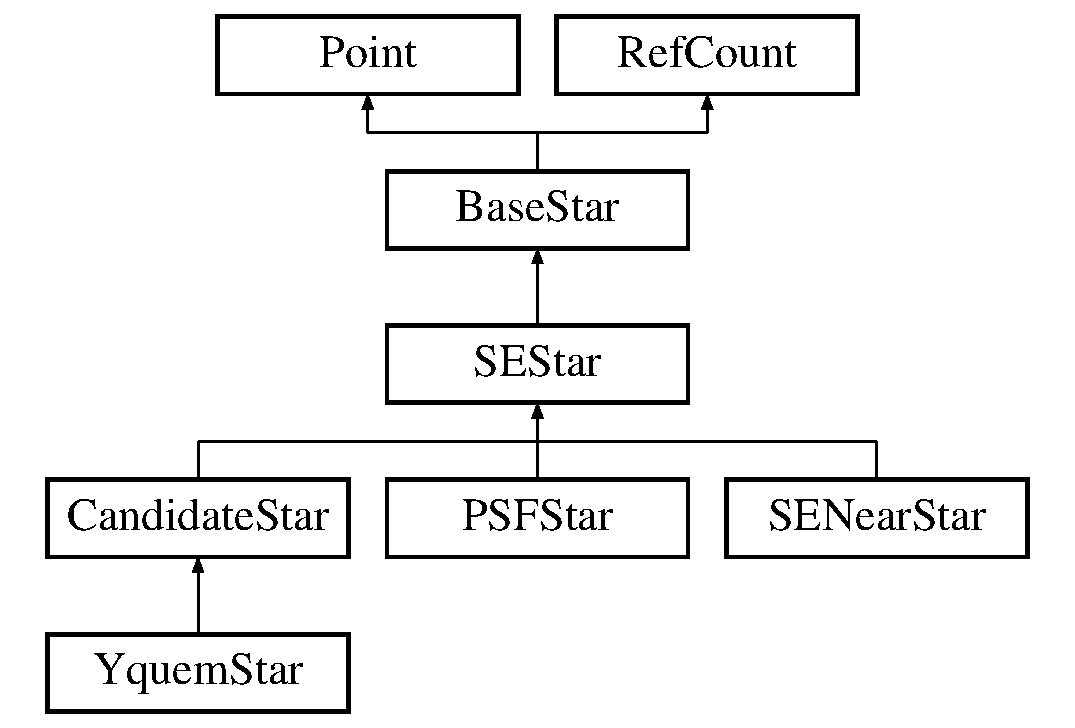
\includegraphics[height=5cm]{class_sestar}
\end{center}
\end{figure}
\subsubsection*{Public Methods}
\begin{CompactItemize}
\item 
\index{SEStar@{SEStar}!SEStar@{SEStar}}\index{SEStar@{SEStar}!SEStar@{SEStar}}
{\bf SEStar} ()\label{class_sestar_a0}

\item 
\index{SEStar@{SEStar}!SEStar@{SEStar}}\index{SEStar@{SEStar}!SEStar@{SEStar}}
{\bf SEStar} (double xx, double yy, double ff)\label{class_sestar_a1}

\item 
\index{HasNeighbours@{HasNeighbours}!SEStar@{SEStar}}\index{SEStar@{SEStar}!HasNeighbours@{Has\-Neighbours}}
bool {\bf Has\-Neighbours} () const\label{class_sestar_a2}

\begin{CompactList}\small\item\em The object has neighbours, bright and close enough to bias aperture photometry.\item\end{CompactList}\item 
\index{IsBlended@{IsBlended}!SEStar@{SEStar}}\index{SEStar@{SEStar}!IsBlended@{Is\-Blended}}
bool {\bf Is\-Blended} () const\label{class_sestar_a3}

\begin{CompactList}\small\item\em The object is blended with another one.\item\end{CompactList}\item 
\index{IsBad@{IsBad}!SEStar@{SEStar}}\index{SEStar@{SEStar}!IsBad@{Is\-Bad}}
bool {\bf Is\-Bad} () const\label{class_sestar_a4}

\item 
\index{IsCosmic@{IsCosmic}!SEStar@{SEStar}}\index{SEStar@{SEStar}!IsCosmic@{Is\-Cosmic}}
bool {\bf Is\-Cosmic} () const\label{class_sestar_a5}

\item 
\index{IsSaturated@{IsSaturated}!SEStar@{SEStar}}\index{SEStar@{SEStar}!IsSaturated@{Is\-Saturated}}
bool {\bf Is\-Saturated} (const double saturation) const\label{class_sestar_a6}

\begin{CompactList}\small\item\em at least one pixel is saturated.\item\end{CompactList}\item 
\index{IsSaturated@{IsSaturated}!SEStar@{SEStar}}\index{SEStar@{SEStar}!IsSaturated@{Is\-Saturated}}
bool {\bf Is\-Saturated} () const\label{class_sestar_a7}

\item 
\index{IsTruncated@{IsTruncated}!SEStar@{SEStar}}\index{SEStar@{SEStar}!IsTruncated@{Is\-Truncated}}
bool {\bf Is\-Truncated} () const\label{class_sestar_a8}

\begin{CompactList}\small\item\em the object is truncated.\item\end{CompactList}\item 
\index{FlagAsSaturated@{FlagAsSaturated}!SEStar@{SEStar}}\index{SEStar@{SEStar}!FlagAsSaturated@{Flag\-As\-Saturated}}
void {\bf Flag\-As\-Saturated} ()\label{class_sestar_a9}

\begin{CompactList}\small\item\em To flag a star as saturated.\item\end{CompactList}\item 
\index{FlagAsCosmic@{FlagAsCosmic}!SEStar@{SEStar}}\index{SEStar@{SEStar}!FlagAsCosmic@{Flag\-As\-Cosmic}}
void {\bf Flag\-As\-Cosmic} ()\label{class_sestar_a10}

\begin{CompactList}\small\item\em To flag a star as cosmic.\item\end{CompactList}\item 
\index{FlagAsNotSaturated@{FlagAsNotSaturated}!SEStar@{SEStar}}\index{SEStar@{SEStar}!FlagAsNotSaturated@{Flag\-As\-Not\-Saturated}}
void {\bf Flag\-As\-Not\-Saturated} ()\label{class_sestar_a11}

\begin{CompactList}\small\item\em To un-flag a star because it is not saturated.\item\end{CompactList}\item 
\index{X_Peak@{X\_\-Peak}!SEStar@{SEStar}}\index{SEStar@{SEStar}!X_Peak@{X\_\-Peak}}
double {\bf X\_\-Peak} () const\label{class_sestar_a12}

\begin{CompactList}\small\item\em x-coordinate of the brightest pixel.\item\end{CompactList}\item 
\index{Y_Peak@{Y\_\-Peak}!SEStar@{SEStar}}\index{SEStar@{SEStar}!Y_Peak@{Y\_\-Peak}}
double {\bf Y\_\-Peak} () const\label{class_sestar_a13}

\begin{CompactList}\small\item\em y-coordinate of the brightest pixel.\item\end{CompactList}\item 
\index{EFlux@{EFlux}!SEStar@{SEStar}}\index{SEStar@{SEStar}!EFlux@{EFlux}}
double {\bf EFlux} () const\label{class_sestar_a14}

\begin{CompactList}\small\item\em RMS error for BEST flux.\item\end{CompactList}\item 
\index{Fluxmax@{Fluxmax}!SEStar@{SEStar}}\index{SEStar@{SEStar}!Fluxmax@{Fluxmax}}
double {\bf Fluxmax} () const\label{class_sestar_a15}

\begin{CompactList}\small\item\em Peak flux $\ast$$\ast$above background$\ast$$\ast$.\item\end{CompactList}\item 
\index{Fond@{Fond}!SEStar@{SEStar}}\index{SEStar@{SEStar}!Fond@{Fond}}
double {\bf Fond} () const\label{class_sestar_a16}

\begin{CompactList}\small\item\em background.\item\end{CompactList}\item 
\index{Flux_aper@{Flux\_\-aper}!SEStar@{SEStar}}\index{SEStar@{SEStar}!Flux_aper@{Flux\_\-aper}}
double {\bf Flux\_\-aper} () const\label{class_sestar_a17}

\begin{CompactList}\small\item\em SExtractor FLUX\_\-AUTO: Flux within a Kron-like elliptical aperture.\item\end{CompactList}\item 
\index{Eflux_aper@{Eflux\_\-aper}!SEStar@{SEStar}}\index{SEStar@{SEStar}!Eflux_aper@{Eflux\_\-aper}}
double {\bf Eflux\_\-aper} () const\label{class_sestar_a18}

\begin{CompactList}\small\item\em SExtractor FLUXERR\_\-AUTO : RMS error for Flux\_\-aper.\item\end{CompactList}\item 
\index{Flux_fixaper@{Flux\_\-fixaper}!SEStar@{SEStar}}\index{SEStar@{SEStar}!Flux_fixaper@{Flux\_\-fixaper}}
double {\bf Flux\_\-fixaper} () const\label{class_sestar_a19}

\item 
\index{Eflux_fixaper@{Eflux\_\-fixaper}!SEStar@{SEStar}}\index{SEStar@{SEStar}!Eflux_fixaper@{Eflux\_\-fixaper}}
double {\bf Eflux\_\-fixaper} () const\label{class_sestar_a20}

\item 
\index{Flux_iso@{Flux\_\-iso}!SEStar@{SEStar}}\index{SEStar@{SEStar}!Flux_iso@{Flux\_\-iso}}
double {\bf Flux\_\-iso} () const\label{class_sestar_a21}

\begin{CompactList}\small\item\em SExtractor FLUX\_\-ISO: isophotal flux.\item\end{CompactList}\item 
\index{Eflux_iso@{Eflux\_\-iso}!SEStar@{SEStar}}\index{SEStar@{SEStar}!Eflux_iso@{Eflux\_\-iso}}
double {\bf Eflux\_\-iso} () const\label{class_sestar_a22}

\begin{CompactList}\small\item\em SExtractor FLUXERR\_\-ISO: error on isophotal flux.\item\end{CompactList}\item 
\index{Flux_isocor@{Flux\_\-isocor}!SEStar@{SEStar}}\index{SEStar@{SEStar}!Flux_isocor@{Flux\_\-isocor}}
double {\bf Flux\_\-isocor} () const\label{class_sestar_a23}

\begin{CompactList}\small\item\em SExtractor FLUX\_\-ISOCOR: isophotal corrected flux.\item\end{CompactList}\item 
\index{Eflux_isocor@{Eflux\_\-isocor}!SEStar@{SEStar}}\index{SEStar@{SEStar}!Eflux_isocor@{Eflux\_\-isocor}}
double {\bf Eflux\_\-isocor} () const\label{class_sestar_a24}

\begin{CompactList}\small\item\em SExtractor FLUXERR\_\-ISOCOR error on isophotal corrected flux.\item\end{CompactList}\item 
\index{Fwhm@{Fwhm}!SEStar@{SEStar}}\index{SEStar@{SEStar}!Fwhm@{Fwhm}}
double {\bf Fwhm} () const\label{class_sestar_a25}

\begin{CompactList}\small\item\em fwhm in pixels.\item\end{CompactList}\item 
\index{Kronradius@{Kronradius}!SEStar@{SEStar}}\index{SEStar@{SEStar}!Kronradius@{Kronradius}}
double {\bf Kronradius} () const\label{class_sestar_a26}

\begin{CompactList}\small\item\em extension of the aperture , in units of A or B.\item\end{CompactList}\item 
\index{Isoarea@{Isoarea}!SEStar@{SEStar}}\index{SEStar@{SEStar}!Isoarea@{Isoarea}}
double {\bf Isoarea} () const\label{class_sestar_a27}

\begin{CompactList}\small\item\em area of lowest isophote en pixels.\item\end{CompactList}\item 
\index{Mxx@{Mxx}!SEStar@{SEStar}}\index{SEStar@{SEStar}!Mxx@{Mxx}}
double {\bf Mxx} () const\label{class_sestar_a28}

\begin{CompactList}\small\item\em $<$\$x$^\wedge$2\$ - $<$x$>$\$\{\}$^\wedge$2\$$>$.\item\end{CompactList}\item 
\index{Myy@{Myy}!SEStar@{SEStar}}\index{SEStar@{SEStar}!Myy@{Myy}}
double {\bf Myy} () const\label{class_sestar_a29}

\begin{CompactList}\small\item\em $<$\$y$^\wedge$2\$ - $<$y$>$\$\{\}$^\wedge$2\$$>$.\item\end{CompactList}\item 
\index{Mxy@{Mxy}!SEStar@{SEStar}}\index{SEStar@{SEStar}!Mxy@{Mxy}}
double {\bf Mxy} () const\label{class_sestar_a30}

\begin{CompactList}\small\item\em $<$xy - $<$x$>$$<$y$>$$>$.\item\end{CompactList}\item 
\index{A@{A}!SEStar@{SEStar}}\index{SEStar@{SEStar}!A@{A}}
double {\bf A} () const\label{class_sestar_a31}

\begin{CompactList}\small\item\em Profile RMS along major axis.\item\end{CompactList}\item 
\index{B@{B}!SEStar@{SEStar}}\index{SEStar@{SEStar}!B@{B}}
double {\bf B} () const\label{class_sestar_a32}

\begin{CompactList}\small\item\em Profile RMS along minor axis.\item\end{CompactList}\item 
\index{Gyr_Angle@{Gyr\_\-Angle}!SEStar@{SEStar}}\index{SEStar@{SEStar}!Gyr_Angle@{Gyr\_\-Angle}}
double {\bf Gyr\_\-Angle} () const\label{class_sestar_a33}

\begin{CompactList}\small\item\em gyration angle of the major axis 0.0 = axis en degres Position angle.\item\end{CompactList}\item 
\index{Flag@{Flag}!SEStar@{SEStar}}\index{SEStar@{SEStar}!Flag@{Flag}}
int {\bf Flag} () const\label{class_sestar_a34}

\begin{CompactList}\small\item\em Extraction flags.\item\end{CompactList}\item 
\index{FlagBad@{FlagBad}!SEStar@{SEStar}}\index{SEStar@{SEStar}!FlagBad@{Flag\-Bad}}
int {\bf Flag\-Bad} () const\label{class_sestar_a35}

\begin{CompactList}\small\item\em number of bad pixels in iso area.\item\end{CompactList}\item 
\index{Cstar@{Cstar}!SEStar@{SEStar}}\index{SEStar@{SEStar}!Cstar@{Cstar}}
double {\bf Cstar} () const\label{class_sestar_a36}

\begin{CompactList}\small\item\em star/galaxy classification: [0=gal ... 1=star].\item\end{CompactList}\item 
\index{Xtrunc@{Xtrunc}!SEStar@{SEStar}}\index{SEStar@{SEStar}!Xtrunc@{Xtrunc}}
double {\bf Xtrunc} () const\label{class_sestar_a37}

\begin{CompactList}\small\item\em local barycenter (see Pierre).\item\end{CompactList}\item 
\index{Ytrunc@{Ytrunc}!SEStar@{SEStar}}\index{SEStar@{SEStar}!Ytrunc@{Ytrunc}}
double {\bf Ytrunc} () const\label{class_sestar_a38}

\begin{CompactList}\small\item\em local barycenter.\item\end{CompactList}\item 
\index{N@{N}!SEStar@{SEStar}}\index{SEStar@{SEStar}!N@{N}}
int {\bf N} () const\label{class_sestar_a39}

\item 
\index{Iter@{Iter}!SEStar@{SEStar}}\index{SEStar@{SEStar}!Iter@{Iter}}
int {\bf Iter} () const\label{class_sestar_a40}

\begin{CompactList}\small\item\em Number of iteration in the PSF fitting (ALLSTAR) procedure.\item\end{CompactList}\item 
\index{Chi@{Chi}!SEStar@{SEStar}}\index{SEStar@{SEStar}!Chi@{Chi}}
double {\bf Chi} () const\label{class_sestar_a41}

\begin{CompactList}\small\item\em chi from fit (to be plot vs. magnitude).\item\end{CompactList}\item 
\index{Sharp@{Sharp}!SEStar@{SEStar}}\index{SEStar@{SEStar}!Sharp@{Sharp}}
double {\bf Sharp} () const\label{class_sestar_a42}

\begin{CompactList}\small\item\em sharp diagnostic (to be plot vs. magnitude).\item\end{CompactList}\item 
\index{X_Peak@{X\_\-Peak}!SEStar@{SEStar}}\index{SEStar@{SEStar}!X_Peak@{X\_\-Peak}}
double\& {\bf X\_\-Peak} ()\label{class_sestar_a43}

\item 
\index{Y_Peak@{Y\_\-Peak}!SEStar@{SEStar}}\index{SEStar@{SEStar}!Y_Peak@{Y\_\-Peak}}
double\& {\bf Y\_\-Peak} ()\label{class_sestar_a44}

\item 
\index{EFlux@{EFlux}!SEStar@{SEStar}}\index{SEStar@{SEStar}!EFlux@{EFlux}}
double\& {\bf EFlux} ()\label{class_sestar_a45}

\item 
\index{Fluxmax@{Fluxmax}!SEStar@{SEStar}}\index{SEStar@{SEStar}!Fluxmax@{Fluxmax}}
double\& {\bf Fluxmax} ()\label{class_sestar_a46}

\item 
\index{Fond@{Fond}!SEStar@{SEStar}}\index{SEStar@{SEStar}!Fond@{Fond}}
double\& {\bf Fond} ()\label{class_sestar_a47}

\item 
\index{Flux_aper@{Flux\_\-aper}!SEStar@{SEStar}}\index{SEStar@{SEStar}!Flux_aper@{Flux\_\-aper}}
double\& {\bf Flux\_\-aper} ()\label{class_sestar_a48}

\item 
\index{Eflux_aper@{Eflux\_\-aper}!SEStar@{SEStar}}\index{SEStar@{SEStar}!Eflux_aper@{Eflux\_\-aper}}
double\& {\bf Eflux\_\-aper} ()\label{class_sestar_a49}

\item 
\index{Flux_fixaper@{Flux\_\-fixaper}!SEStar@{SEStar}}\index{SEStar@{SEStar}!Flux_fixaper@{Flux\_\-fixaper}}
double\& {\bf Flux\_\-fixaper} ()\label{class_sestar_a50}

\item 
\index{Eflux_fixaper@{Eflux\_\-fixaper}!SEStar@{SEStar}}\index{SEStar@{SEStar}!Eflux_fixaper@{Eflux\_\-fixaper}}
double\& {\bf Eflux\_\-fixaper} ()\label{class_sestar_a51}

\item 
\index{Flux_iso@{Flux\_\-iso}!SEStar@{SEStar}}\index{SEStar@{SEStar}!Flux_iso@{Flux\_\-iso}}
double\& {\bf Flux\_\-iso} ()\label{class_sestar_a52}

\item 
\index{Eflux_iso@{Eflux\_\-iso}!SEStar@{SEStar}}\index{SEStar@{SEStar}!Eflux_iso@{Eflux\_\-iso}}
double\& {\bf Eflux\_\-iso} ()\label{class_sestar_a53}

\item 
\index{Flux_isocor@{Flux\_\-isocor}!SEStar@{SEStar}}\index{SEStar@{SEStar}!Flux_isocor@{Flux\_\-isocor}}
double\& {\bf Flux\_\-isocor} ()\label{class_sestar_a54}

\item 
\index{Eflux_isocor@{Eflux\_\-isocor}!SEStar@{SEStar}}\index{SEStar@{SEStar}!Eflux_isocor@{Eflux\_\-isocor}}
double\& {\bf Eflux\_\-isocor} ()\label{class_sestar_a55}

\item 
\index{Fwhm@{Fwhm}!SEStar@{SEStar}}\index{SEStar@{SEStar}!Fwhm@{Fwhm}}
double\& {\bf Fwhm} ()\label{class_sestar_a56}

\item 
\index{Kronradius@{Kronradius}!SEStar@{SEStar}}\index{SEStar@{SEStar}!Kronradius@{Kronradius}}
double\& {\bf Kronradius} ()\label{class_sestar_a57}

\item 
\index{Isoarea@{Isoarea}!SEStar@{SEStar}}\index{SEStar@{SEStar}!Isoarea@{Isoarea}}
double\& {\bf Isoarea} ()\label{class_sestar_a58}

\item 
\index{Mxx@{Mxx}!SEStar@{SEStar}}\index{SEStar@{SEStar}!Mxx@{Mxx}}
double\& {\bf Mxx} ()\label{class_sestar_a59}

\item 
\index{Myy@{Myy}!SEStar@{SEStar}}\index{SEStar@{SEStar}!Myy@{Myy}}
double\& {\bf Myy} ()\label{class_sestar_a60}

\item 
\index{Mxy@{Mxy}!SEStar@{SEStar}}\index{SEStar@{SEStar}!Mxy@{Mxy}}
double\& {\bf Mxy} ()\label{class_sestar_a61}

\item 
\index{A@{A}!SEStar@{SEStar}}\index{SEStar@{SEStar}!A@{A}}
double\& {\bf A} ()\label{class_sestar_a62}

\item 
\index{B@{B}!SEStar@{SEStar}}\index{SEStar@{SEStar}!B@{B}}
double\& {\bf B} ()\label{class_sestar_a63}

\item 
\index{Gyr_Angle@{Gyr\_\-Angle}!SEStar@{SEStar}}\index{SEStar@{SEStar}!Gyr_Angle@{Gyr\_\-Angle}}
double\& {\bf Gyr\_\-Angle} ()\label{class_sestar_a64}

\item 
\index{Flag@{Flag}!SEStar@{SEStar}}\index{SEStar@{SEStar}!Flag@{Flag}}
int\& {\bf Flag} ()\label{class_sestar_a65}

\item 
\index{FlagBad@{FlagBad}!SEStar@{SEStar}}\index{SEStar@{SEStar}!FlagBad@{Flag\-Bad}}
int\& {\bf Flag\-Bad} ()\label{class_sestar_a66}

\item 
\index{Cstar@{Cstar}!SEStar@{SEStar}}\index{SEStar@{SEStar}!Cstar@{Cstar}}
double\& {\bf Cstar} ()\label{class_sestar_a67}

\item 
\index{Xtrunc@{Xtrunc}!SEStar@{SEStar}}\index{SEStar@{SEStar}!Xtrunc@{Xtrunc}}
double\& {\bf Xtrunc} ()\label{class_sestar_a68}

\item 
\index{Ytrunc@{Ytrunc}!SEStar@{SEStar}}\index{SEStar@{SEStar}!Ytrunc@{Ytrunc}}
double\& {\bf Ytrunc} ()\label{class_sestar_a69}

\item 
\index{N@{N}!SEStar@{SEStar}}\index{SEStar@{SEStar}!N@{N}}
int\& {\bf N} ()\label{class_sestar_a70}

\item 
\index{Iter@{Iter}!SEStar@{SEStar}}\index{SEStar@{SEStar}!Iter@{Iter}}
int\& {\bf Iter} ()\label{class_sestar_a71}

\item 
\index{Chi@{Chi}!SEStar@{SEStar}}\index{SEStar@{SEStar}!Chi@{Chi}}
double\& {\bf Chi} ()\label{class_sestar_a72}

\item 
\index{Sharp@{Sharp}!SEStar@{SEStar}}\index{SEStar@{SEStar}!Sharp@{Sharp}}
double\& {\bf Sharp} ()\label{class_sestar_a73}

\item 
\index{dumpn@{dumpn}!SEStar@{SEStar}}\index{SEStar@{SEStar}!dumpn@{dumpn}}
virtual void {\bf dumpn} (ostream \&s=cout) const\label{class_sestar_a74}

\begin{CompactList}\small\item\em for dump with NO end-of-line.\item\end{CompactList}\item 
\index{dump@{dump}!SEStar@{SEStar}}\index{SEStar@{SEStar}!dump@{dump}}
virtual void {\bf dump} (ostream \&s=cout) const\label{class_sestar_a75}

\begin{CompactList}\small\item\em for dump.\item\end{CompactList}\item 
\index{writen@{writen}!SEStar@{SEStar}}\index{SEStar@{SEStar}!writen@{writen}}
virtual void {\bf writen} (ostream \&s=cout) const\label{class_sestar_a76}

\begin{CompactList}\small\item\em for write with NO end-of-line.\item\end{CompactList}\item 
\index{read_it@{read\_\-it}!SEStar@{SEStar}}\index{SEStar@{SEStar}!read_it@{read\_\-it}}
virtual void {\bf read\_\-it} (istream \&r, const char $\ast$Format)\label{class_sestar_a77}

\begin{CompactList}\small\item\em to read once the object is created.\item\end{CompactList}\item 
\index{WriteHeader_@{WriteHeader\_\-}!SEStar@{SEStar}}\index{SEStar@{SEStar}!WriteHeader_@{Write\-Header\_\-}}
std::string {\bf Write\-Header\_\-} (ostream \&pr=cout, const char $\ast$i=NULL) const\label{class_sestar_a78}

\item 
\index{IsOK@{IsOK}!SEStar@{SEStar}}\index{SEStar@{SEStar}!IsOK@{Is\-OK}}
bool {\bf Is\-OK} (const double \&saturation) const\label{class_sestar_a79}

\end{CompactItemize}
\subsubsection*{Static Public Methods}
\begin{CompactItemize}
\item 
\index{read@{read}!SEStar@{SEStar}}\index{SEStar@{SEStar}!read@{read}}
SEStar$\ast$ {\bf read} (istream \&r, const char $\ast$Format)\label{class_sestar_d0}

\begin{CompactList}\small\item\em to read and create the object.\item\end{CompactList}\item 
\index{TypeName@{TypeName}!SEStar@{SEStar}}\index{SEStar@{SEStar}!TypeName@{Type\-Name}}
const char$\ast$ {\bf Type\-Name} ()\label{class_sestar_d1}

\end{CompactItemize}
\subsubsection*{Protected Attributes}
\begin{CompactItemize}
\item 
\index{num@{num}!SEStar@{SEStar}}\index{SEStar@{SEStar}!num@{num}}
int {\bf num}\label{class_sestar_n0}

\item 
\index{xpeak@{xpeak}!SEStar@{SEStar}}\index{SEStar@{SEStar}!xpeak@{xpeak}}
double {\bf xpeak}\label{class_sestar_n1}

\item 
\index{ypeak@{ypeak}!SEStar@{SEStar}}\index{SEStar@{SEStar}!ypeak@{ypeak}}
double {\bf ypeak}\label{class_sestar_n2}

\item 
\index{fluxmax@{fluxmax}!SEStar@{SEStar}}\index{SEStar@{SEStar}!fluxmax@{fluxmax}}
double {\bf fluxmax}\label{class_sestar_n3}

\item 
\index{e_flux@{e\_\-flux}!SEStar@{SEStar}}\index{SEStar@{SEStar}!e_flux@{e\_\-flux}}
double {\bf e\_\-flux}\label{class_sestar_n4}

\item 
\index{fond@{fond}!SEStar@{SEStar}}\index{SEStar@{SEStar}!fond@{fond}}
double {\bf fond}\label{class_sestar_n5}

\item 
\index{flux_aper@{flux\_\-aper}!SEStar@{SEStar}}\index{SEStar@{SEStar}!flux_aper@{flux\_\-aper}}
double {\bf flux\_\-aper}\label{class_sestar_n6}

\item 
\index{e_flux_aper@{e\_\-flux\_\-aper}!SEStar@{SEStar}}\index{SEStar@{SEStar}!e_flux_aper@{e\_\-flux\_\-aper}}
double {\bf e\_\-flux\_\-aper}\label{class_sestar_n7}

\item 
\index{flux_fixaper@{flux\_\-fixaper}!SEStar@{SEStar}}\index{SEStar@{SEStar}!flux_fixaper@{flux\_\-fixaper}}
double {\bf flux\_\-fixaper}\label{class_sestar_n8}

\item 
\index{e_flux_fixaper@{e\_\-flux\_\-fixaper}!SEStar@{SEStar}}\index{SEStar@{SEStar}!e_flux_fixaper@{e\_\-flux\_\-fixaper}}
double {\bf e\_\-flux\_\-fixaper}\label{class_sestar_n9}

\item 
\index{flux_iso@{flux\_\-iso}!SEStar@{SEStar}}\index{SEStar@{SEStar}!flux_iso@{flux\_\-iso}}
double {\bf flux\_\-iso}\label{class_sestar_n10}

\item 
\index{e_flux_iso@{e\_\-flux\_\-iso}!SEStar@{SEStar}}\index{SEStar@{SEStar}!e_flux_iso@{e\_\-flux\_\-iso}}
double {\bf e\_\-flux\_\-iso}\label{class_sestar_n11}

\item 
\index{flux_isocor@{flux\_\-isocor}!SEStar@{SEStar}}\index{SEStar@{SEStar}!flux_isocor@{flux\_\-isocor}}
double {\bf flux\_\-isocor}\label{class_sestar_n12}

\item 
\index{e_flux_isocor@{e\_\-flux\_\-isocor}!SEStar@{SEStar}}\index{SEStar@{SEStar}!e_flux_isocor@{e\_\-flux\_\-isocor}}
double {\bf e\_\-flux\_\-isocor}\label{class_sestar_n13}

\item 
\index{kronradius@{kronradius}!SEStar@{SEStar}}\index{SEStar@{SEStar}!kronradius@{kronradius}}
double {\bf kronradius}\label{class_sestar_n14}

\item 
\index{isoarea@{isoarea}!SEStar@{SEStar}}\index{SEStar@{SEStar}!isoarea@{isoarea}}
double {\bf isoarea}\label{class_sestar_n15}

\item 
\index{fwhm@{fwhm}!SEStar@{SEStar}}\index{SEStar@{SEStar}!fwhm@{fwhm}}
double {\bf fwhm}\label{class_sestar_n16}

\item 
\index{mxx@{mxx}!SEStar@{SEStar}}\index{SEStar@{SEStar}!mxx@{mxx}}
double {\bf mxx}\label{class_sestar_n17}

\item 
\index{myy@{myy}!SEStar@{SEStar}}\index{SEStar@{SEStar}!myy@{myy}}
double {\bf myy}\label{class_sestar_n18}

\item 
\index{mxy@{mxy}!SEStar@{SEStar}}\index{SEStar@{SEStar}!mxy@{mxy}}
double {\bf mxy}\label{class_sestar_n19}

\item 
\index{a@{a}!SEStar@{SEStar}}\index{SEStar@{SEStar}!a@{a}}
double {\bf a}\label{class_sestar_n20}

\item 
\index{b@{b}!SEStar@{SEStar}}\index{SEStar@{SEStar}!b@{b}}
double {\bf b}\label{class_sestar_n21}

\item 
\index{gyr_angle@{gyr\_\-angle}!SEStar@{SEStar}}\index{SEStar@{SEStar}!gyr_angle@{gyr\_\-angle}}
double {\bf gyr\_\-angle}\label{class_sestar_n22}

\item 
\index{flag@{flag}!SEStar@{SEStar}}\index{SEStar@{SEStar}!flag@{flag}}
int {\bf flag}\label{class_sestar_n23}

\item 
\index{flagbad@{flagbad}!SEStar@{SEStar}}\index{SEStar@{SEStar}!flagbad@{flagbad}}
int {\bf flagbad}\label{class_sestar_n24}

\item 
\index{cstar@{cstar}!SEStar@{SEStar}}\index{SEStar@{SEStar}!cstar@{cstar}}
double {\bf cstar}\label{class_sestar_n25}

\item 
\index{xtrunc@{xtrunc}!SEStar@{SEStar}}\index{SEStar@{SEStar}!xtrunc@{xtrunc}}
double {\bf xtrunc}\label{class_sestar_n26}

\item 
\index{ytrunc@{ytrunc}!SEStar@{SEStar}}\index{SEStar@{SEStar}!ytrunc@{ytrunc}}
double {\bf ytrunc}\label{class_sestar_n27}

\item 
\index{iter@{iter}!SEStar@{SEStar}}\index{SEStar@{SEStar}!iter@{iter}}
int {\bf iter}\label{class_sestar_n28}

\item 
\index{chi@{chi}!SEStar@{SEStar}}\index{SEStar@{SEStar}!chi@{chi}}
double {\bf chi}\label{class_sestar_n29}

\item 
\index{sharp@{sharp}!SEStar@{SEStar}}\index{SEStar@{SEStar}!sharp@{sharp}}
double {\bf sharp}\label{class_sestar_n30}

\end{CompactItemize}


\subsubsection{Detailed Description}
SExtractor star.

The flux of {\bf Base\-Star} {\rm (p.\,\pageref{class_basestar})} is FLUX\_\-BEST from SExtractor, i.e. FLUX\_\-ISOCOR if not crowded, FLUX\_\-AUTO otherwise. 



The documentation for this class was generated from the following files:\begin{CompactItemize}
\item 
{\bf sestar.h}\item 
sestar.cc\end{CompactItemize}

\subsection{Simultaneous\-Fit  Class Reference}
\label{class_simultaneousfit}\index{SimultaneousFit@{Simultaneous\-Fit}}
Simultaneous fitting of Vignets. 


{\tt \#include $<$simultaneousfit.h$>$}

Inheritance diagram for Simultaneous\-Fit::\begin{figure}[H]
\begin{center}
\leavevmode
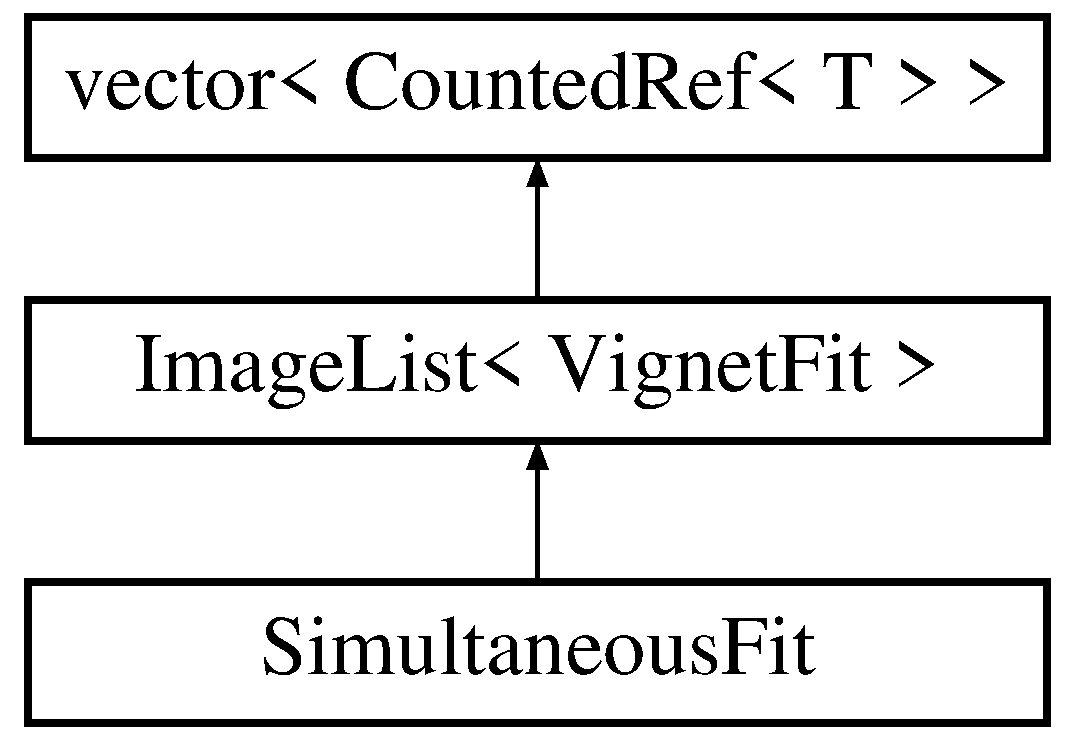
\includegraphics[height=3cm]{class_simultaneousfit}
\end{center}
\end{figure}
\subsubsection*{Public Methods}
\begin{CompactItemize}
\item 
\index{SimultaneousFit@{SimultaneousFit}!SimultaneousFit@{Simultaneous\-Fit}}\index{SimultaneousFit@{SimultaneousFit}!SimultaneousFit@{Simultaneous\-Fit}}
{\bf Simultaneous\-Fit} ()\label{class_simultaneousfit_a0}

\item 
\index{~SimultaneousFit@{$\sim$SimultaneousFit}!SimultaneousFit@{Simultaneous\-Fit}}\index{SimultaneousFit@{SimultaneousFit}!~SimultaneousFit@{$\sim$Simultaneous\-Fit}}
{\bf $\sim$Simultaneous\-Fit} ()\label{class_simultaneousfit_a1}

\item 
\index{FillMatAndVec@{FillMatAndVec}!SimultaneousFit@{Simultaneous\-Fit}}\index{SimultaneousFit@{SimultaneousFit}!FillMatAndVec@{Fill\-Mat\-And\-Vec}}
void {\bf Fill\-Mat\-And\-Vec} ()\label{class_simultaneousfit_a2}

\begin{CompactList}\small\item\em fill the entire matrix and vectors.\item\end{CompactList}\item 
\index{Solve@{Solve}!SimultaneousFit@{Simultaneous\-Fit}}\index{SimultaneousFit@{SimultaneousFit}!Solve@{Solve}}
bool {\bf Solve} (const double \&lambda=0, const bool invert=false)\label{class_simultaneousfit_a3}

\begin{CompactList}\small\item\em solve the linear equation system.\item\end{CompactList}\item 
\index{IterateAndSolve@{IterateAndSolve}!SimultaneousFit@{Simultaneous\-Fit}}\index{SimultaneousFit@{SimultaneousFit}!IterateAndSolve@{Iterate\-And\-Solve}}
bool {\bf Iterate\-And\-Solve} (const int Max\-Iterations, const double Epsilon=0.01)\label{class_simultaneousfit_a4}

\begin{CompactList}\small\item\em iterate on solution and solve the system.\item\end{CompactList}\item 
\index{AssignStar@{AssignStar}!SimultaneousFit@{Simultaneous\-Fit}}\index{SimultaneousFit@{SimultaneousFit}!AssignStar@{Assign\-Star}}
void {\bf Assign\-Star} ()\label{class_simultaneousfit_a5}

\begin{CompactList}\small\item\em assign the Vignet\-Fit star.\item\end{CompactList}\item 
\index{ComputeChi2@{ComputeChi2}!SimultaneousFit@{Simultaneous\-Fit}}\index{SimultaneousFit@{SimultaneousFit}!ComputeChi2@{Compute\-Chi2}}
double {\bf Compute\-Chi2} ()\label{class_simultaneousfit_a6}

\begin{CompactList}\small\item\em compute total chi2 and residuals of the fit.\item\end{CompactList}\item 
\index{ApplyCorrections@{ApplyCorrections}!SimultaneousFit@{Simultaneous\-Fit}}\index{SimultaneousFit@{SimultaneousFit}!ApplyCorrections@{Apply\-Corrections}}
bool {\bf Apply\-Corrections} (const double Factor=1)\label{class_simultaneousfit_a7}

\begin{CompactList}\small\item\em apply corrections of the last solution with a scale factor.\item\end{CompactList}\item 
\index{MakeResidsAndWeights@{MakeResidsAndWeights}!SimultaneousFit@{Simultaneous\-Fit}}\index{SimultaneousFit@{SimultaneousFit}!MakeResidsAndWeights@{Make\-Resids\-And\-Weights}}
void {\bf Make\-Resids\-And\-Weights} ()\label{class_simultaneousfit_a8}

\begin{CompactList}\small\item\em update all vignets from last model fitted and resid.\item\end{CompactList}\item 
\index{MakePsfs@{MakePsfs}!SimultaneousFit@{Simultaneous\-Fit}}\index{SimultaneousFit@{SimultaneousFit}!MakePsfs@{Make\-Psfs}}
void {\bf Make\-Psfs} ()\label{class_simultaneousfit_a9}

\begin{CompactList}\small\item\em redo all vignets integrated and convolved psfs and derivatives at the last fitted position.\item\end{CompactList}\item 
\index{DoTheFit@{DoTheFit}!SimultaneousFit@{Simultaneous\-Fit}}\index{SimultaneousFit@{SimultaneousFit}!DoTheFit@{Do\-The\-Fit}}
void {\bf Do\-The\-Fit} (const double \&Max\-Scale=1)\label{class_simultaneousfit_a10}

\begin{CompactList}\small\item\em fill, fit and shit.\item\end{CompactList}\item 
\index{SetWhatToFit@{SetWhatToFit}!SimultaneousFit@{Simultaneous\-Fit}}\index{SimultaneousFit@{SimultaneousFit}!SetWhatToFit@{Set\-What\-To\-Fit}}
void {\bf Set\-What\-To\-Fit} (const int To\-Fit=Fit\-Flux$|$Fit\-Gal)\label{class_simultaneousfit_a11}

\begin{CompactList}\small\item\em set what you want to fit.\item\end{CompactList}\item 
\index{FindMinimumScale@{FindMinimumScale}!SimultaneousFit@{Simultaneous\-Fit}}\index{SimultaneousFit@{SimultaneousFit}!FindMinimumScale@{Find\-Minimum\-Scale}}
void {\bf Find\-Minimum\-Scale} (const double \&Worst\-Seeing)\label{class_simultaneousfit_a12}

\begin{CompactList}\small\item\em get the minimum scaling factor to resize the vignets.\item\end{CompactList}\item 
\index{MakeInitialModel@{MakeInitialModel}!SimultaneousFit@{Simultaneous\-Fit}}\index{SimultaneousFit@{SimultaneousFit}!MakeInitialModel@{Make\-Initial\-Model}}
void {\bf Make\-Initial\-Model} ()\label{class_simultaneousfit_a13}

\begin{CompactList}\small\item\em build a rough initial galaxy to start the iterative fit.\item\end{CompactList}\item 
\index{Resize@{Resize}!SimultaneousFit@{Simultaneous\-Fit}}\index{SimultaneousFit@{SimultaneousFit}!Resize@{Resize}}
void {\bf Resize} (const double \&Scale\-Factor)\label{class_simultaneousfit_a14}

\begin{CompactList}\small\item\em resize all the vignets of a scale factor.\item\end{CompactList}\item 
\index{GetGalaxyFlux@{GetGalaxyFlux}!SimultaneousFit@{Simultaneous\-Fit}}\index{SimultaneousFit@{SimultaneousFit}!GetGalaxyFlux@{Get\-Galaxy\-Flux}}
double {\bf Get\-Galaxy\-Flux} (double \&Var\-Gal\-Flux) const\label{class_simultaneousfit_a15}

\begin{CompactList}\small\item\em compute galaxy flux consistently with the rest.\item\end{CompactList}\item 
\index{GetZeroFlux@{GetZeroFlux}!SimultaneousFit@{Simultaneous\-Fit}}\index{SimultaneousFit@{SimultaneousFit}!GetZeroFlux@{Get\-Zero\-Flux}}
double {\bf Get\-Zero\-Flux} (double \&Var\-Zero\-Flux) const\label{class_simultaneousfit_a16}

\begin{CompactList}\small\item\em compute zero flux as weighted average of zero nights.\item\end{CompactList}\item 
\index{write@{write}!SimultaneousFit@{Simultaneous\-Fit}}\index{SimultaneousFit@{SimultaneousFit}!write@{write}}
void {\bf write} (const string \&Middle\-Name) const\label{class_simultaneousfit_a17}

\begin{CompactList}\small\item\em write.\item\end{CompactList}\item 
\index{Chi2@{Chi2}!SimultaneousFit@{Simultaneous\-Fit}}\index{SimultaneousFit@{SimultaneousFit}!Chi2@{Chi2}}
double {\bf Chi2} () const\label{class_simultaneousfit_a18}

\begin{CompactList}\small\item\em returns total chi2 of the fit.\item\end{CompactList}\item 
\index{GetChi2@{GetChi2}!SimultaneousFit@{Simultaneous\-Fit}}\index{SimultaneousFit@{SimultaneousFit}!GetChi2@{Get\-Chi2}}
void {\bf Get\-Chi2} (double \&newchi2, const double \&oldchi2, double \&lambda)\label{class_simultaneousfit_a19}

\item 
\index{Dof@{Dof}!SimultaneousFit@{Simultaneous\-Fit}}\index{SimultaneousFit@{SimultaneousFit}!Dof@{Dof}}
int {\bf Dof} () const\label{class_simultaneousfit_a20}

\begin{CompactList}\small\item\em returns number of degrees of freedom.\item\end{CompactList}\item 
\index{Scale@{Scale}!SimultaneousFit@{Simultaneous\-Fit}}\index{SimultaneousFit@{SimultaneousFit}!Scale@{Scale}}
double {\bf Scale} () const\label{class_simultaneousfit_a21}

\begin{CompactList}\small\item\em returns the current scale factor for vignets.\item\end{CompactList}\end{CompactItemize}
\subsubsection*{Public Attributes}
\begin{CompactItemize}
\item 
\index{Minim@{Minim}!SimultaneousFit@{Simultaneous\-Fit}}\index{SimultaneousFit@{SimultaneousFit}!Minim@{Minim}}
Minim\-Method {\bf Minim}\label{class_simultaneousfit_m0}

\item 
\index{VignetRef@{VignetRef}!SimultaneousFit@{Simultaneous\-Fit}}\index{SimultaneousFit@{SimultaneousFit}!VignetRef@{Vignet\-Ref}}
Vignet\-Fit$\ast$ {\bf Vignet\-Ref}\label{class_simultaneousfit_m1}

\begin{CompactList}\small\item\em pointer to the best seeing vignet.\item\end{CompactList}\item 
\index{galaxy@{galaxy}!SimultaneousFit@{Simultaneous\-Fit}}\index{SimultaneousFit@{SimultaneousFit}!galaxy@{galaxy}}
{\bf Vignet}$\ast$ {\bf galaxy}\label{class_simultaneousfit_m2}

\begin{CompactList}\small\item\em pointer to the reconstructed galaxy centered double image.\item\end{CompactList}\end{CompactItemize}


\subsubsection{Detailed Description}
Simultaneous fitting of Vignets.



The documentation for this class was generated from the following file:\begin{CompactItemize}
\item 
{\bf simultaneousfit.h}\end{CompactItemize}

\subsection{Stamp  Class Reference}
\label{class_stamp}\index{Stamp@{Stamp}}
an odd size {\bf DImage} {\rm (p.\,\pageref{class_dimage})} extracted from an {\bf Image} {\rm (p.\,\pageref{class_image})}, centered on (xc,yc). 


{\tt \#include $<$dimage.h$>$}

\subsubsection*{Public Methods}
\begin{CompactItemize}
\item 
\index{HSize@{HSize}!Stamp@{Stamp}}\index{Stamp@{Stamp}!HSize@{HSize}}
int {\bf HSize} () const\label{class_stamp_a0}

\item 
\index{Stamp@{Stamp}!Stamp@{Stamp}}\index{Stamp@{Stamp}!Stamp@{Stamp}}
{\bf Stamp} (const double Xc, const double Yc, const {\bf Image} \&image, int HStamp\-Size, {\bf Base\-Star} $\ast$Star)\label{class_stamp_a1}

\item 
\index{Stamp@{Stamp}!Stamp@{Stamp}}\index{Stamp@{Stamp}!Stamp@{Stamp}}
{\bf Stamp} ()\label{class_stamp_a2}

\item 
\index{~Stamp@{$\sim$Stamp}!Stamp@{Stamp}}\index{Stamp@{Stamp}!~Stamp@{$\sim$Stamp}}
virtual {\bf $\sim$Stamp} ()\label{class_stamp_a3}

\end{CompactItemize}
\subsubsection*{Public Attributes}
\begin{CompactItemize}
\item 
\index{xc@{xc}!Stamp@{Stamp}}\index{Stamp@{Stamp}!xc@{xc}}
int {\bf xc}\label{class_stamp_m0}

\begin{CompactList}\small\item\em center in the source {\bf Image} {\rm (p.\,\pageref{class_image})}.\item\end{CompactList}\item 
\index{yc@{yc}!Stamp@{Stamp}}\index{Stamp@{Stamp}!yc@{yc}}
int {\bf yc}\label{class_stamp_m1}

\begin{CompactList}\small\item\em center in the source {\bf Image} {\rm (p.\,\pageref{class_image})}.\item\end{CompactList}\item 
\index{xstart@{xstart}!Stamp@{Stamp}}\index{Stamp@{Stamp}!xstart@{xstart}}
int {\bf xstart}\label{class_stamp_m2}

\item 
\index{ystart@{ystart}!Stamp@{Stamp}}\index{Stamp@{Stamp}!ystart@{ystart}}
int {\bf ystart}\label{class_stamp_m3}

\item 
\index{source@{source}!Stamp@{Stamp}}\index{Stamp@{Stamp}!source@{source}}
{\bf DImage} {\bf source}\label{class_stamp_m4}

\begin{CompactList}\small\item\em pixels (in double precision until one changes DPixel definition ).\item\end{CompactList}\item 
\index{chi2@{chi2}!Stamp@{Stamp}}\index{Stamp@{Stamp}!chi2@{chi2}}
double {\bf chi2}\label{class_stamp_m5}

\begin{CompactList}\small\item\em will be filled and used to discard outliers from the fit.\item\end{CompactList}\item 
\index{star@{star}!Stamp@{Stamp}}\index{Stamp@{Stamp}!star@{star}}
Base\-Star\-Ref {\bf star}\label{class_stamp_m6}

\begin{CompactList}\small\item\em we should not assume that there is a {\bf Base\-Star} {\rm (p.\,\pageref{class_basestar})} corresponding to this stamp, but if any, put its pointer here.\item\end{CompactList}\end{CompactItemize}


\subsubsection{Detailed Description}
an odd size {\bf DImage} {\rm (p.\,\pageref{class_dimage})} extracted from an {\bf Image} {\rm (p.\,\pageref{class_image})}, centered on (xc,yc).



The documentation for this class was generated from the following file:\begin{CompactItemize}
\item 
{\bf dimage.h}\end{CompactItemize}

\subsection{Stamp\-List  Class Reference}
\label{class_stamplist}\index{StampList@{Stamp\-List}}
Nothing but a list of Stamps. 


{\tt \#include $<$dimage.h$>$}

Inheritance diagram for Stamp\-List::\begin{figure}[H]
\begin{center}
\leavevmode
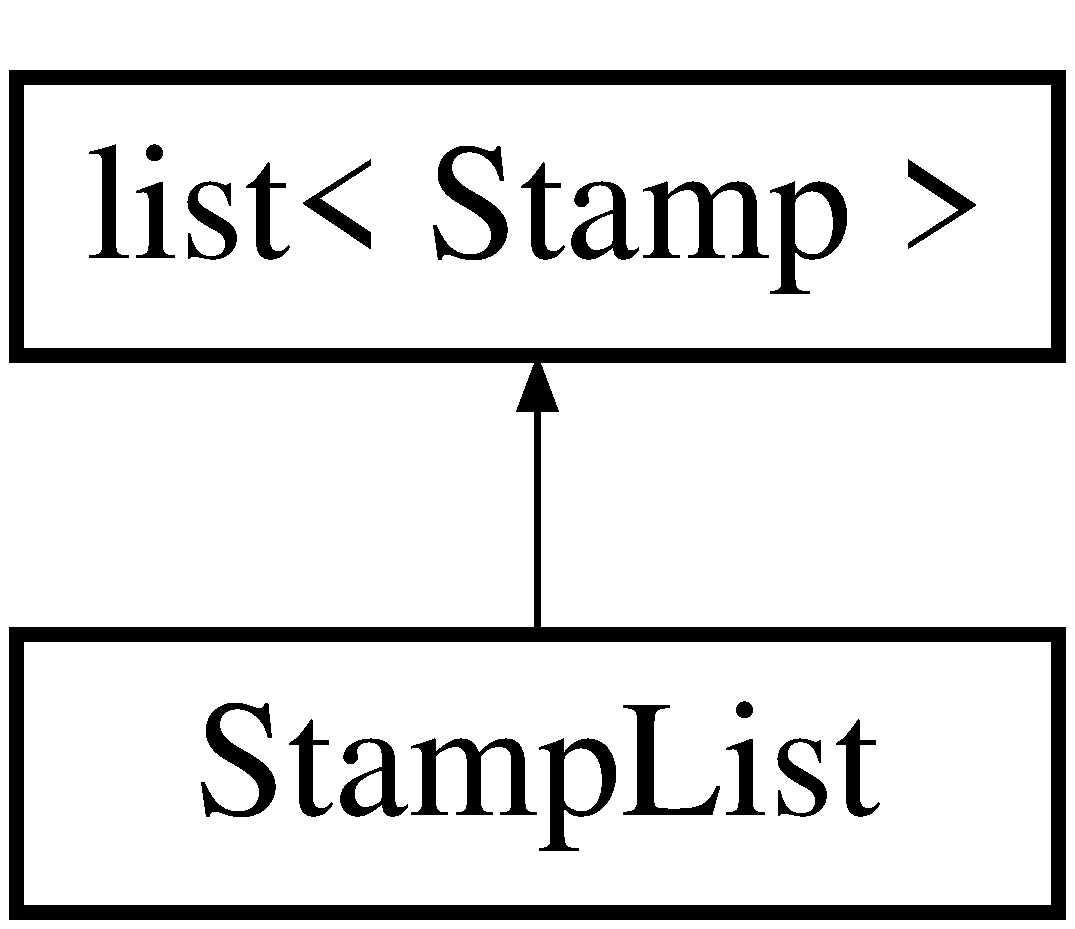
\includegraphics[height=2cm]{class_stamplist}
\end{center}
\end{figure}
\subsubsection*{Public Methods}
\begin{CompactItemize}
\item 
\index{StampList@{StampList}!StampList@{Stamp\-List}}\index{StampList@{StampList}!StampList@{Stamp\-List}}
{\bf Stamp\-List} (const {\bf Image} \&image, const Base\-Star\-List \&star\-List, const int h\-Stamp\-Size, const int Max\-Stamps)\label{class_stamplist_a0}

\item 
\index{~StampList@{$\sim$StampList}!StampList@{Stamp\-List}}\index{StampList@{StampList}!~StampList@{$\sim$Stamp\-List}}
virtual {\bf $\sim$Stamp\-List} ()\label{class_stamplist_a1}

\end{CompactItemize}


\subsubsection{Detailed Description}
Nothing but a list of Stamps.



The documentation for this class was generated from the following file:\begin{CompactItemize}
\item 
{\bf dimage.h}\end{CompactItemize}

\subsection{Star\-List  Class Template Reference}
\label{class_starlist}\index{StarList@{Star\-List}}
lists of Stars. 


{\tt \#include $<$starlist.h$>$}

Inheritance diagram for Star\-List::\begin{figure}[H]
\begin{center}
\leavevmode
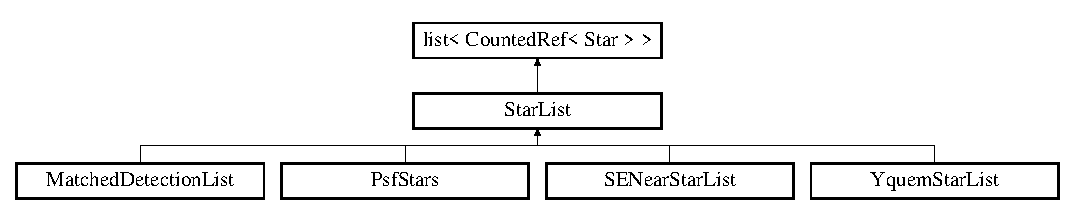
\includegraphics[height=2.44186cm]{class_starlist}
\end{center}
\end{figure}
\subsubsection*{Public Types}
\begin{CompactItemize}
\item 
\index{Element@{Element}!StarList@{Star\-List}}\index{StarList@{StarList}!Element@{Element}}
typedef {\bf Counted\-Ref}$<$Star$>$ {\bf Element}\label{class_starlist_s0}

\item 
\index{StarCIterator@{StarCIterator}!StarList@{Star\-List}}\index{StarList@{StarList}!StarCIterator@{Star\-CIterator}}
typedef list$<$Element$>$::const\_\-iterator {\bf Star\-CIterator}\label{class_starlist_s1}

\item 
\index{StarIterator@{StarIterator}!StarList@{Star\-List}}\index{StarList@{StarList}!StarIterator@{Star\-Iterator}}
typedef list$<$Element$>$::iterator {\bf Star\-Iterator}\label{class_starlist_s2}

\end{CompactItemize}
\subsubsection*{Public Methods}
\begin{CompactItemize}
\item 
\index{StarList@{StarList}!StarList@{Star\-List}}\index{StarList@{StarList}!StarList@{Star\-List}}
{\bf Star\-List} ()\label{class_starlist_a0}

\begin{CompactList}\small\item\em : default constructor (empty list).\item\end{CompactList}\item 
{\bf Star\-List} (const string \&File\-Name)
\begin{CompactList}\small\item\em reads a Star\-List from a file,.\item\end{CompactList}\item 
int {\bf write} (const string \&File\-Name)
\begin{CompactList}\small\item\em writes to a file.\item\end{CompactList}\item 
\index{read@{read}!StarList@{Star\-List}}\index{StarList@{StarList}!read@{read}}
int {\bf read} (const string \&File\-Name)\label{class_starlist_a3}

\begin{CompactList}\small\item\em obvious meaning.\item\end{CompactList}\item 
\index{push_back@{push\_\-back}!StarList@{Star\-List}}\index{StarList@{StarList}!push_back@{push\_\-back}}
void {\bf push\_\-back} (Star $\ast$t)\label{class_starlist_a4}

\item 
\index{push_back@{push\_\-back}!StarList@{Star\-List}}\index{StarList@{StarList}!push_back@{push\_\-back}}
void {\bf push\_\-back} (const Element \&e)\label{class_starlist_a5}

\item 
\index{~StarList@{$\sim$StarList}!StarList@{Star\-List}}\index{StarList@{StarList}!~StarList@{$\sim$Star\-List}}
virtual {\bf $\sim$Star\-List} ()\label{class_starlist_a6}

\item 
\index{dump@{dump}!StarList@{Star\-List}}\index{StarList@{StarList}!dump@{dump}}
void {\bf dump} (ostream \&stream=cout) const\label{class_starlist_a7}

\begin{CompactList}\small\item\em invokes dump(stream) for all Stars in the list.\item\end{CompactList}\item 
void {\bf Flux\-Sort} ()
\begin{CompactList}\small\item\em a model routine to sort the list.\item\end{CompactList}\item 
\index{ExtractHead@{ExtractHead}!StarList@{Star\-List}}\index{StarList@{StarList}!ExtractHead@{Extract\-Head}}
void {\bf Extract\-Head} (Star\-List$<$ Star $>$ \&Out, int NHead) const\label{class_starlist_a9}

\begin{CompactList}\small\item\em copy the head of the list at the end of an other list (that may be empty on input).\item\end{CompactList}\item 
\index{CutTail@{CutTail}!StarList@{Star\-List}}\index{StarList@{StarList}!CutTail@{Cut\-Tail}}
void {\bf Cut\-Tail} (const int NKeep)\label{class_starlist_a10}

\begin{CompactList}\small\item\em cuts the end of the list.\item\end{CompactList}\item 
\index{ExtractInFrame@{ExtractInFrame}!StarList@{Star\-List}}\index{StarList@{StarList}!ExtractInFrame@{Extract\-In\-Frame}}
void {\bf Extract\-In\-Frame} (Star\-List$<$ Star $>$ \&Out, const {\bf Frame} \&a\-Frame) const\label{class_starlist_a11}

\begin{CompactList}\small\item\em copy the part of the list which is included in the frame at the end of another list.\item\end{CompactList}\item 
\index{CutEdges@{CutEdges}!StarList@{Star\-List}}\index{StarList@{StarList}!CutEdges@{Cut\-Edges}}
void {\bf Cut\-Edges} (const {\bf Frame} \&a\-Frame, float mindist)\label{class_starlist_a12}

\begin{CompactList}\small\item\em cut the part of the list which is at a distance $<$ mindist of the edges defined by frame.\item\end{CompactList}\item 
\index{CopyTo@{CopyTo}!StarList@{Star\-List}}\index{StarList@{StarList}!CopyTo@{Copy\-To}}
void {\bf Copy\-To} (Star\-List$<$ Star $>$ \&Copy) const\label{class_starlist_a13}

\begin{CompactList}\small\item\em clears Copy and makes a copy of the list to Copy.\item\end{CompactList}\item 
\index{ClearList@{ClearList}!StarList@{Star\-List}}\index{StarList@{StarList}!ClearList@{Clear\-List}}
void {\bf Clear\-List} ()\label{class_starlist_a14}

\begin{CompactList}\small\item\em Clears the list.\item\end{CompactList}\item 
template$<$class Operator$>$ void {\bf Apply\-Transfo} (const Operator \&Op)
\begin{CompactList}\small\item\em enables to apply a geometrical transfo if Star is Basestar or derives from it.\item\end{CompactList}\item 
\index{FindClosest@{FindClosest}!StarList@{Star\-List}}\index{StarList@{StarList}!FindClosest@{Find\-Closest}}
Star$\ast$ {\bf Find\-Closest} (double X, double Y) const\label{class_starlist_a16}

\begin{CompactList}\small\item\em returns the closest Star from a given location.\item\end{CompactList}\item 
\index{FindClosest@{FindClosest}!StarList@{Star\-List}}\index{StarList@{StarList}!FindClosest@{Find\-Closest}}
Star$\ast$ {\bf Find\-Closest} (const {\bf Point} \&P) const\label{class_starlist_a17}

\begin{CompactList}\small\item\em same as above. Can be used with any of our star-like stuff.\item\end{CompactList}\item 
\index{HasCloseNeighbor@{HasCloseNeighbor}!StarList@{Star\-List}}\index{StarList@{StarList}!HasCloseNeighbor@{Has\-Close\-Neighbor}}
bool {\bf Has\-Close\-Neighbor} (double X, double Y, double maxdist, double mindist=0.1) const\label{class_starlist_a18}

\begin{CompactList}\small\item\em true if location has a nearby star in a ring between mindist and maxdist.\item\end{CompactList}\item 
\index{HasCloseNeighbor@{HasCloseNeighbor}!StarList@{Star\-List}}\index{StarList@{StarList}!HasCloseNeighbor@{Has\-Close\-Neighbor}}
bool {\bf Has\-Close\-Neighbor} (const {\bf Point} \&P, double maxdist, double mindist=0.1) const\label{class_starlist_a19}

\begin{CompactList}\small\item\em same as above. Can be used with any of our star-like stuff.\item\end{CompactList}\item 
\index{ClosestNeighbor@{ClosestNeighbor}!StarList@{Star\-List}}\index{StarList@{StarList}!ClosestNeighbor@{Closest\-Neighbor}}
Star$\ast$ {\bf Closest\-Neighbor} (double X, double Y, double mindist=0.1) const\label{class_starlist_a20}

\begin{CompactList}\small\item\em nearby star to a star but not itself.\item\end{CompactList}\item 
\index{ClosestNeighbor@{ClosestNeighbor}!StarList@{Star\-List}}\index{StarList@{StarList}!ClosestNeighbor@{Closest\-Neighbor}}
Star$\ast$ {\bf Closest\-Neighbor} (const {\bf Point} \&P, double mindist=0.1) const\label{class_starlist_a21}

\begin{CompactList}\small\item\em same as above. Can be used with any of our star-like stuff.\item\end{CompactList}\item 
\index{NumberOfNeighbors@{NumberOfNeighbors}!StarList@{Star\-List}}\index{StarList@{StarList}!NumberOfNeighbors@{Number\-Of\-Neighbors}}
int {\bf Number\-Of\-Neighbors} (const double \&X, const double \&Y, const double \&distmax) const\label{class_starlist_a22}

\item 
\index{AllNeighbors@{AllNeighbors}!StarList@{Star\-List}}\index{StarList@{StarList}!AllNeighbors@{All\-Neighbors}}
int {\bf All\-Neighbors} (Star\-List \&Neighbor\-List, const double \&X, const double \&Y, const double \&distmax) const\label{class_starlist_a23}

\item 
\index{AllNeighbors@{AllNeighbors}!StarList@{Star\-List}}\index{StarList@{StarList}!AllNeighbors@{All\-Neighbors}}
int {\bf All\-Neighbors} (Star\-List \&Neighbor\-List, const {\bf Point} \&Pt, const double \&distmax) const\label{class_starlist_a24}

\item 
\index{NumberOfNeighbors@{NumberOfNeighbors}!StarList@{Star\-List}}\index{StarList@{StarList}!NumberOfNeighbors@{Number\-Of\-Neighbors}}
int {\bf Number\-Of\-Neighbors} (const {\bf Point} \&Pt, const double \&distmax) const\label{class_starlist_a25}

\end{CompactItemize}
\subsubsection*{Protected Methods}
\begin{CompactItemize}
\item 
\index{ascii_read@{ascii\_\-read}!StarList@{Star\-List}}\index{StarList@{StarList}!ascii_read@{ascii\_\-read}}
int {\bf ascii\_\-read} (const string \&File\-Name)\label{class_starlist_b0}

\end{CompactItemize}


\subsubsection{Detailed Description}
\subsubsection*{template$<$class Star$>$  class Star\-List}

lists of Stars.

It is a template class, which means that the Star type remains undefined until a user defines it.  The list related operations (insertion, sort, traversal) are to be carried out using STL  list operations. Most of the Star operations rely on routines to be provided in  the Star class, usually user defined. The instanciation of this class for  {\bf Base\-Star} {\rm (p.\,\pageref{class_basestar})} (i.e. the replacement  of the formal parameter 'Star' by '{\bf Base\-Star} {\rm (p.\,\pageref{class_basestar})}') is  called Base\-Star\-List.  Take care: what is stored is pointers on Star's and  NOT Star's. This implies that Stars being inserted in the list have to be  obtained using 'new'. The corresponding 'delete' are invoked in the destructor. 



\subsubsection{Constructor \& Destructor Documentation}
\index{StarList@{Star\-List}!StarList@{StarList}}
\index{StarList@{StarList}!StarList@{Star\-List}}
\paragraph{\setlength{\rightskip}{0pt plus 5cm}template$<$class Star$>$ Star\-List$<$Star$>$::Star\-List$<$Star$>$ (const string \& {\em File\-Name})}\hfill\label{class_starlist_a1}


reads a Star\-List from a file,.

using the read method from the Star class.  See {\bf Base\-Star} {\rm (p.\,\pageref{class_basestar})} for an example of implementation. 

\subsubsection{Member Function Documentation}
\index{StarList@{Star\-List}!ApplyTransfo@{ApplyTransfo}}
\index{ApplyTransfo@{ApplyTransfo}!StarList@{Star\-List}}
\paragraph{\setlength{\rightskip}{0pt plus 5cm}template$<$class Star$>$  template$<$class Operator$>$ void Star\-List$<$Star$>$::Apply\-Transfo (const Operator \& {\em Op})\hspace{0.3cm}{\tt  [inline]}}\hfill\label{class_starlist_a15}


enables to apply a geometrical transfo if Star is Basestar or derives from it.

could be extended to other type of transformations. \index{StarList@{Star\-List}!FluxSort@{FluxSort}}
\index{FluxSort@{FluxSort}!StarList@{Star\-List}}
\paragraph{\setlength{\rightskip}{0pt plus 5cm}template$<$class Star$>$ void Star\-List$<$Star$>$::Flux\-Sort ()\hspace{0.3cm}{\tt  [inline]}}\hfill\label{class_starlist_a8}


a model routine to sort the list.

see {\bf Decreasing\-Flux}() {\rm (p.\,\pageref{basestar_h_a7})} to see what it is, if you  want another sorting criterion) \index{StarList@{Star\-List}!write@{write}}
\index{write@{write}!StarList@{Star\-List}}
\paragraph{\setlength{\rightskip}{0pt plus 5cm}template$<$class Star$>$ int Star\-List$<$Star$>$::write (const string \& {\em File\-Name})}\hfill\label{class_starlist_a2}


writes to a file.

calls iteratively the write method of the Star  class. It is unusable if the Star class does not  provide this functionnality. see {\bf Base\-Star} {\rm (p.\,\pageref{class_basestar})} to see a possible implementation.  not const because the write routines of Root are not 

The documentation for this class was generated from the following file:\begin{CompactItemize}
\item 
{\bf starlist.h}\end{CompactItemize}

\subsection{Star\-Match  Class Reference}
\label{class_starmatch}\index{StarMatch@{Star\-Match}}
a pair of stars, usually belonging to different images. 


{\tt \#include $<$starmatch.h$>$}

\subsubsection*{Public Methods}
\begin{CompactItemize}
\item 
{\bf Star\-Match} (const {\bf Point} \&p1, const {\bf Point} \&p2, const {\bf Base\-Star} $\ast$S1, const {\bf Base\-Star} $\ast$S2)
\begin{CompactList}\small\item\em constructor.\item\end{CompactList}\item 
\index{Distance@{Distance}!StarMatch@{Star\-Match}}\index{StarMatch@{StarMatch}!Distance@{Distance}}
double {\bf Distance} (const {\bf Gtransfo} \&T) const\label{class_starmatch_a1}

\begin{CompactList}\small\item\em returns the distance from T(p1) to p2.\item\end{CompactList}\item 
\index{SetDistance@{SetDistance}!StarMatch@{Star\-Match}}\index{StarMatch@{StarMatch}!SetDistance@{Set\-Distance}}
void {\bf Set\-Distance} (const {\bf Gtransfo} \&T)\label{class_starmatch_a2}

\begin{CompactList}\small\item\em to be used before sorting on distances.\item\end{CompactList}\item 
\index{Distance@{Distance}!StarMatch@{Star\-Match}}\index{StarMatch@{StarMatch}!Distance@{Distance}}
double {\bf Distance} () const\label{class_starmatch_a3}

\begin{CompactList}\small\item\em returns the value computed by the above one.\item\end{CompactList}\item 
\index{Swap@{Swap}!StarMatch@{Star\-Match}}\index{StarMatch@{StarMatch}!Swap@{Swap}}
void {\bf Swap} ()\label{class_starmatch_a4}

\item 
\index{StarMatch@{StarMatch}!StarMatch@{Star\-Match}}\index{StarMatch@{StarMatch}!StarMatch@{Star\-Match}}
{\bf Star\-Match} ()\label{class_starmatch_a5}

\item 
\index{~StarMatch@{$\sim$StarMatch}!StarMatch@{Star\-Match}}\index{StarMatch@{StarMatch}!~StarMatch@{$\sim$Star\-Match}}
{\bf $\sim$Star\-Match} ()\label{class_starmatch_a6}

\end{CompactItemize}
\subsubsection*{Public Attributes}
\begin{CompactItemize}
\item 
\index{point1@{point1}!StarMatch@{Star\-Match}}\index{StarMatch@{StarMatch}!point1@{point1}}
{\bf Point} {\bf point1}\label{class_starmatch_m0}

\item 
\index{point2@{point2}!StarMatch@{Star\-Match}}\index{StarMatch@{StarMatch}!point2@{point2}}
{\bf Point} {\bf point2}\label{class_starmatch_m1}

\begin{CompactList}\small\item\em 2 points.\item\end{CompactList}\item 
\index{s1@{s1}!StarMatch@{Star\-Match}}\index{StarMatch@{StarMatch}!s1@{s1}}
Base\-Star\-Ref {\bf s1}\label{class_starmatch_m2}

\item 
\index{s2@{s2}!StarMatch@{Star\-Match}}\index{StarMatch@{StarMatch}!s2@{s2}}
Base\-Star\-Ref {\bf s2}\label{class_starmatch_m3}

\begin{CompactList}\small\item\em the Star pointers (the pointer is in fact generic, pointed data is never used).\item\end{CompactList}\item 
\index{distance@{distance}!StarMatch@{Star\-Match}}\index{StarMatch@{StarMatch}!distance@{distance}}
double {\bf distance}\label{class_starmatch_m4}

\end{CompactItemize}
\subsubsection*{Friends}
\begin{CompactItemize}
\item 
class {\bf Star\-Match\-List}
\item 
class {\bf Dec\-Flux}
\item 
class {\bf Increasing\-Distances}
\item 
class {\bf Decreasing\-Distances}
\item 
class {\bf operator$<$$<$}
\item 
class {\bf Compare\-S1}
\item 
class {\bf Same\-S1}
\item 
class {\bf Compare\-S2}
\item 
class {\bf Same\-S2}
\end{CompactItemize}


\subsubsection{Detailed Description}
a pair of stars, usually belonging to different images.

One would normally assume that they are the same object of the sky. The object contains basically two 2d points (called later p1 and p2), and two pointers (unused by the class and its satellites), that enable in the end to trace back the stars in the caller data structures. 



\subsubsection{Constructor \& Destructor Documentation}
\index{StarMatch@{Star\-Match}!StarMatch@{StarMatch}}
\index{StarMatch@{StarMatch}!StarMatch@{Star\-Match}}
\paragraph{\setlength{\rightskip}{0pt plus 5cm}Star\-Match::Star\-Match (const {\bf Point} \& {\em p1}, const {\bf Point} \& {\em p2}, const {\bf Base\-Star} $\ast$ {\em S1}, const {\bf Base\-Star} $\ast$ {\em S2})\hspace{0.3cm}{\tt  [inline]}}\hfill\label{class_starmatch_a0}


constructor.

gives 2 points (that contain the geometry), plus pointers to the Star objects (which are there for user convenience). 

The documentation for this class was generated from the following file:\begin{CompactItemize}
\item 
{\bf starmatch.h}\end{CompactItemize}

\subsection{Sub  Class Reference}
\label{class_sub}\index{Sub@{Sub}}
Handling of an actual subtraction (shift-coadd-subtract-detect). See {\bf Syntax of the \char`\"{}subfile\char`\"{}} {\rm (p.\,\pageref{subfile})} for the way to drive it. 


{\tt \#include $<$sub.h$>$}

\subsubsection*{Public Methods}
\begin{CompactItemize}
\item 
\index{Sub@{Sub}!Sub@{Sub}}\index{Sub@{Sub}!Sub@{Sub}}
{\bf Sub} (const string \&Sub\-File\-Name, const bool Overwrite=false, const bool Only\-Det=false)\label{class_sub_a0}

\begin{CompactList}\small\item\em the constructor. see {\bf Syntax of the \char`\"{}subfile\char`\"{}} {\rm (p.\,\pageref{subfile})} for the syntax of the \char`\"{}subfile\char`\"{}.\item\end{CompactList}\item 
\index{~Sub@{$\sim$Sub}!Sub@{Sub}}\index{Sub@{Sub}!~Sub@{$\sim$Sub}}
{\bf $\sim$Sub} ()\label{class_sub_a1}

\item 
\index{ExtractSubimage@{ExtractSubimage}!Sub@{Sub}}\index{Sub@{Sub}!ExtractSubimage@{Extract\-Subimage}}
{\bf Reduced\-Image}$\ast$ {\bf Extract\-Subimage} (const string \&Sub\-Image\-Name)\label{class_sub_a2}

\item 
\index{RemoveImage@{RemoveImage}!Sub@{Sub}}\index{Sub@{Sub}!RemoveImage@{Remove\-Image}}
void {\bf Remove\-Image} (const string \&To\-Remove)\label{class_sub_a3}

\item 
\index{SubstituteName@{SubstituteName}!Sub@{Sub}}\index{Sub@{Sub}!SubstituteName@{Substitute\-Name}}
void {\bf Substitute\-Name} (const string \&Original, const string \&Substitution)\label{class_sub_a4}

\item 
\index{DoIt@{DoIt}!Sub@{Sub}}\index{Sub@{Sub}!DoIt@{Do\-It}}
int {\bf Do\-It} ()\label{class_sub_a5}

\item 
\index{ExpectedMagLim@{ExpectedMagLim}!Sub@{Sub}}\index{Sub@{Sub}!ExpectedMagLim@{Expected\-Mag\-Lim}}
int {\bf Expected\-Mag\-Lim} ()\label{class_sub_a6}

\item 
\index{DoOneStack@{DoOneStack}!Sub@{Sub}}\index{Sub@{Sub}!DoOneStack@{Do\-One\-Stack}}
{\bf Reduced\-Image}$\ast$ {\bf Do\-One\-Stack} (String\-List Components, const string \&Stack\-Name, int To\-Do)\label{class_sub_a7}

\item 
\index{FindGeometricReference@{FindGeometricReference}!Sub@{Sub}}\index{Sub@{Sub}!FindGeometricReference@{Find\-Geometric\-Reference}}
void {\bf Find\-Geometric\-Reference} ()\label{class_sub_a8}

\item 
\index{CheckNewNames@{CheckNewNames}!Sub@{Sub}}\index{Sub@{Sub}!CheckNewNames@{Check\-New\-Names}}
int {\bf Check\-New\-Names} ()\label{class_sub_a9}

\item 
\index{RunDetection@{RunDetection}!Sub@{Sub}}\index{Sub@{Sub}!RunDetection@{Run\-Detection}}
void {\bf Run\-Detection} ()\label{class_sub_a10}

\end{CompactItemize}


\subsubsection{Detailed Description}
Handling of an actual subtraction (shift-coadd-subtract-detect). See {\bf Syntax of the \char`\"{}subfile\char`\"{}} {\rm (p.\,\pageref{subfile})} for the way to drive it.



The documentation for this class was generated from the following file:\begin{CompactItemize}
\item 
{\bf sub.h}\end{CompactItemize}

\subsection{Sub\-Image  Class Reference}
\label{class_subimage}\index{SubImage@{Sub\-Image}}
a class that allows to cut a subimage from a {\bf Reduced\-Image} {\rm (p.\,\pageref{class_reducedimage})}. 


{\tt \#include $<$subimage.h$>$}

Inheritance diagram for Sub\-Image::\begin{figure}[H]
\begin{center}
\leavevmode
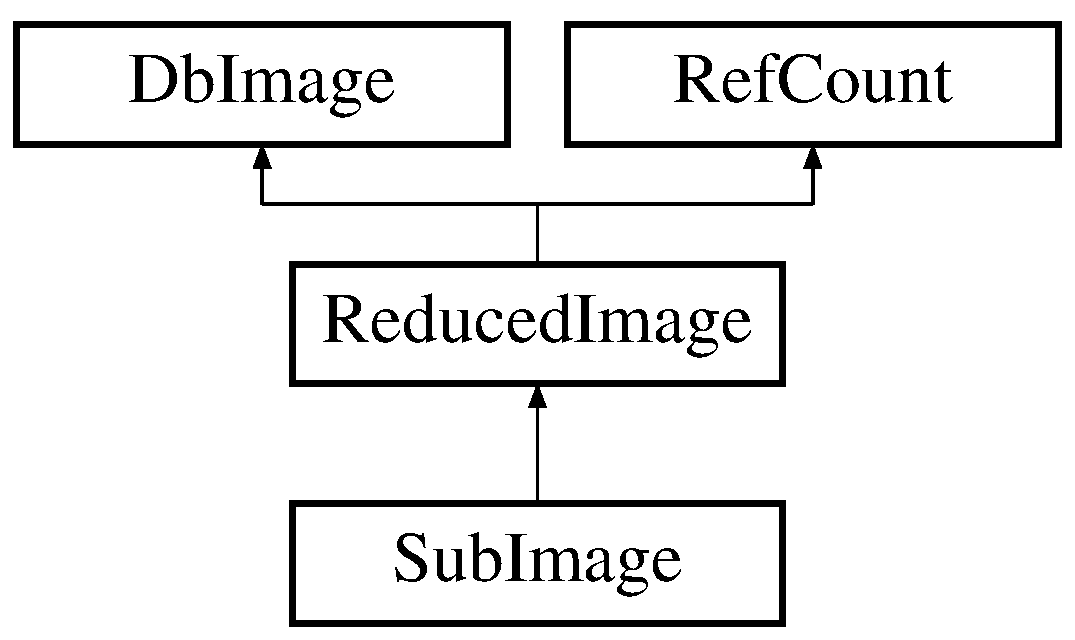
\includegraphics[height=3cm]{class_subimage}
\end{center}
\end{figure}
\subsubsection*{Public Methods}
\begin{CompactItemize}
\item 
\index{SubImage@{SubImage}!SubImage@{Sub\-Image}}\index{SubImage@{SubImage}!SubImage@{Sub\-Image}}
{\bf Sub\-Image} ()\label{class_subimage_a0}

\item 
\index{SubImage@{SubImage}!SubImage@{Sub\-Image}}\index{SubImage@{SubImage}!SubImage@{Sub\-Image}}
{\bf Sub\-Image} (const string \&Name, const string \&Large\-Image\-Name, const {\bf Frame} \&Sub\-Frame)\label{class_subimage_a1}

\item 
\index{MakeFits@{MakeFits}!SubImage@{Sub\-Image}}\index{SubImage@{SubImage}!MakeFits@{Make\-Fits}}
bool {\bf Make\-Fits} ()\label{class_subimage_a2}

\begin{CompactList}\small\item\em produce fits image.\item\end{CompactList}\item 
\index{MakeWeight@{MakeWeight}!SubImage@{Sub\-Image}}\index{SubImage@{SubImage}!MakeWeight@{Make\-Weight}}
bool {\bf Make\-Weight} ()\label{class_subimage_a3}

\item 
\index{MakeCosmic@{MakeCosmic}!SubImage@{Sub\-Image}}\index{SubImage@{SubImage}!MakeCosmic@{Make\-Cosmic}}
bool {\bf Make\-Cosmic} ()\label{class_subimage_a4}

\begin{CompactList}\small\item\em produce cosmic image.\item\end{CompactList}\item 
\index{MakeSatellite@{MakeSatellite}!SubImage@{Sub\-Image}}\index{SubImage@{SubImage}!MakeSatellite@{Make\-Satellite}}
bool {\bf Make\-Satellite} ()\label{class_subimage_a5}

\begin{CompactList}\small\item\em produce satellite image.\item\end{CompactList}\item 
\index{MakeSatur@{MakeSatur}!SubImage@{Sub\-Image}}\index{SubImage@{SubImage}!MakeSatur@{Make\-Satur}}
bool {\bf Make\-Satur} ()\label{class_subimage_a6}

\begin{CompactList}\small\item\em produce satur image.\item\end{CompactList}\item 
\index{MakeDead@{MakeDead}!SubImage@{Sub\-Image}}\index{SubImage@{SubImage}!MakeDead@{Make\-Dead}}
bool {\bf Make\-Dead} ()\label{class_subimage_a7}

\begin{CompactList}\small\item\em produce dead image.\item\end{CompactList}\item 
\index{MakeCatalog@{MakeCatalog}!SubImage@{Sub\-Image}}\index{SubImage@{SubImage}!MakeCatalog@{Make\-Catalog}}
bool {\bf Make\-Catalog} ()\label{class_subimage_a8}

\begin{CompactList}\small\item\em Produce the Saturated stars pixels mask, subtract the image background, detect with the SExtractor computed sigma. search the cosmics, and update catalog and weight for cosmics. No free coffee.\item\end{CompactList}\item 
\index{Clone@{Clone}!SubImage@{Sub\-Image}}\index{SubImage@{SubImage}!Clone@{Clone}}
{\bf Reduced\-Image}$\ast$ {\bf Clone} () const\label{class_subimage_a9}

\end{CompactItemize}


\subsubsection{Detailed Description}
a class that allows to cut a subimage from a {\bf Reduced\-Image} {\rm (p.\,\pageref{class_reducedimage})}.



The documentation for this class was generated from the following file:\begin{CompactItemize}
\item 
{\bf subimage.h}\end{CompactItemize}

\subsection{Tan\-Pix2Ra\-Dec  Class Reference}
\label{class_tanpix2radec}\index{TanPix2RaDec@{Tan\-Pix2Ra\-Dec}}
the transformation that handles pix to sideral transfos (Gnomonic, possibly with polynomial distortions). 


{\tt \#include $<$gtransfo.h$>$}

Inheritance diagram for Tan\-Pix2Ra\-Dec::\begin{figure}[H]
\begin{center}
\leavevmode
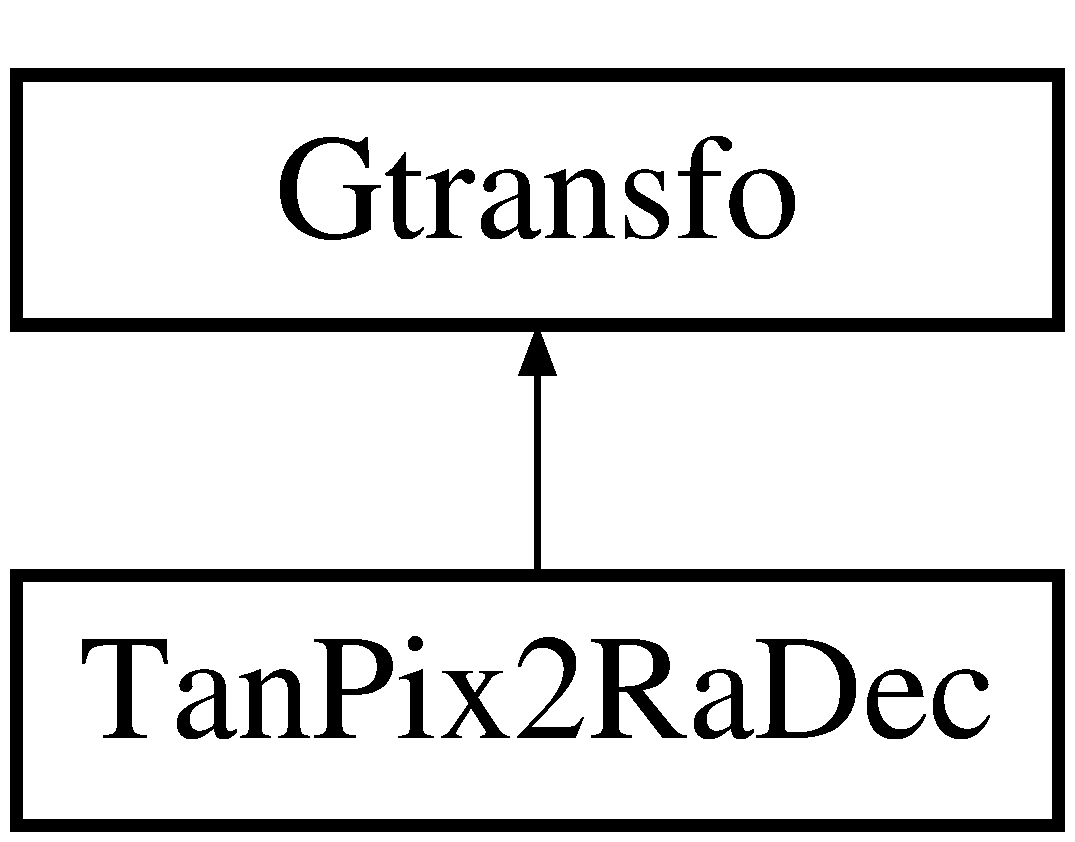
\includegraphics[height=2cm]{class_tanpix2radec}
\end{center}
\end{figure}
\subsubsection*{Public Methods}
\begin{CompactItemize}
\item 
\index{TanPix2RaDec@{TanPix2RaDec}!TanPix2RaDec@{Tan\-Pix2Ra\-Dec}}\index{TanPix2RaDec@{TanPix2RaDec}!TanPix2RaDec@{Tan\-Pix2Ra\-Dec}}
{\bf Tan\-Pix2Ra\-Dec} (const {\bf Gtransfo\-Lin} \&Pix2Tan, const {\bf Point} \&Tangent\-Point, const {\bf Gtransfo\-Quad} $\ast$Corrections=NULL)\label{class_tanpix2radec_a0}

\begin{CompactList}\small\item\em Pix2Tan describes the transfo from pix to tangent plane (in degrees). Tangent\-Point in degrees. Corrections are applied between Lin and deprojection parts (as in Swarp).\item\end{CompactList}\item 
\index{TanPix2RaDec@{TanPix2RaDec}!TanPix2RaDec@{Tan\-Pix2Ra\-Dec}}\index{TanPix2RaDec@{TanPix2RaDec}!TanPix2RaDec@{Tan\-Pix2Ra\-Dec}}
{\bf Tan\-Pix2Ra\-Dec} (const Tan\-Pix2Ra\-Dec \&Original)\label{class_tanpix2radec_a1}

\item 
\index{operator=@{operator=}!TanPix2RaDec@{Tan\-Pix2Ra\-Dec}}\index{TanPix2RaDec@{TanPix2RaDec}!operator=@{operator=}}
void {\bf operator=} (const Tan\-Pix2Ra\-Dec \&)\label{class_tanpix2radec_a2}

\item 
\index{TanPix2RaDec@{TanPix2RaDec}!TanPix2RaDec@{Tan\-Pix2Ra\-Dec}}\index{TanPix2RaDec@{TanPix2RaDec}!TanPix2RaDec@{Tan\-Pix2Ra\-Dec}}
{\bf Tan\-Pix2Ra\-Dec} ()\label{class_tanpix2radec_a3}

\item 
\index{apply@{apply}!TanPix2RaDec@{Tan\-Pix2Ra\-Dec}}\index{TanPix2RaDec@{TanPix2RaDec}!apply@{apply}}
void {\bf apply} (const double Xin, const double Yin, double \&Xout, double \&Yout) const\label{class_tanpix2radec_a4}

\item 
\index{apply@{apply}!TanPix2RaDec@{Tan\-Pix2Ra\-Dec}}\index{TanPix2RaDec@{TanPix2RaDec}!apply@{apply}}
{\bf Point} {\bf apply} (const {\bf Point} \&Pin) const\label{class_tanpix2radec_a5}

\item 
\index{operator *@{operator $\ast$}!TanPix2RaDec@{Tan\-Pix2Ra\-Dec}}\index{TanPix2RaDec@{TanPix2RaDec}!operator *@{operator $\ast$}}
Tan\-Pix2Ra\-Dec {\bf operator $\ast$} (const {\bf Gtransfo\-Lin} \&Right)\label{class_tanpix2radec_a6}

\begin{CompactList}\small\item\em composition with {\bf Gtransfo\-Lin} {\rm (p.\,\pageref{class_gtransfolin})}.\item\end{CompactList}\item 
\index{invert@{invert}!TanPix2RaDec@{Tan\-Pix2Ra\-Dec}}\index{TanPix2RaDec@{TanPix2RaDec}!invert@{invert}}
{\bf Tan\-Ra\-Dec2Pix} {\bf invert} () const\label{class_tanpix2radec_a7}

\begin{CompactList}\small\item\em approximate inverse : it ignores corrections;.\item\end{CompactList}\item 
\index{RoughInverse@{RoughInverse}!TanPix2RaDec@{Tan\-Pix2Ra\-Dec}}\index{TanPix2RaDec@{TanPix2RaDec}!RoughInverse@{Rough\-Inverse}}
{\bf Gtransfo}$\ast$ {\bf Rough\-Inverse} (const {\bf Frame} \&Region) const\label{class_tanpix2radec_a8}

\begin{CompactList}\small\item\em Overload the \char`\"{}generic routine\char`\"{} (available for all {\bf Gtransfo} {\rm (p.\,\pageref{class_gtransfo})} types.\item\end{CompactList}\item 
\index{InverseTransfo@{InverseTransfo}!TanPix2RaDec@{Tan\-Pix2Ra\-Dec}}\index{TanPix2RaDec@{TanPix2RaDec}!InverseTransfo@{Inverse\-Transfo}}
{\bf Gtransfo}$\ast$ {\bf Inverse\-Transfo} (const double Precision, const {\bf Frame} \&Region) const\label{class_tanpix2radec_a9}

\begin{CompactList}\small\item\em Inverse transfo: returns a {\bf Tan\-Ra\-Dec2Pix} {\rm (p.\,\pageref{class_tanradec2pix})} if there are no corrections, or the iterative solver if there are.\item\end{CompactList}\item 
\index{SetCorrections@{SetCorrections}!TanPix2RaDec@{Tan\-Pix2Ra\-Dec}}\index{TanPix2RaDec@{TanPix2RaDec}!SetCorrections@{Set\-Corrections}}
void {\bf Set\-Corrections} (const {\bf Gtransfo\-Quad} $\ast$Corrections)\label{class_tanpix2radec_a10}

\begin{CompactList}\small\item\em Sets the corrections (it can be a cubic ocrrection).\item\end{CompactList}\item 
\index{Clone@{Clone}!TanPix2RaDec@{Tan\-Pix2Ra\-Dec}}\index{TanPix2RaDec@{TanPix2RaDec}!Clone@{Clone}}
{\bf Gtransfo}$\ast$ {\bf Clone} () const\label{class_tanpix2radec_a11}

\begin{CompactList}\small\item\em returns a copy (allocated by new) of the transformation.\item\end{CompactList}\item 
\index{dump@{dump}!TanPix2RaDec@{Tan\-Pix2Ra\-Dec}}\index{TanPix2RaDec@{TanPix2RaDec}!dump@{dump}}
void {\bf dump} (ostream \&stream) const\label{class_tanpix2radec_a12}

\begin{CompactList}\small\item\em dumps the transfo coefficients to stream.\item\end{CompactList}\item 
\index{TangentPoint@{TangentPoint}!TanPix2RaDec@{Tan\-Pix2Ra\-Dec}}\index{TanPix2RaDec@{TanPix2RaDec}!TangentPoint@{Tangent\-Point}}
{\bf Point} {\bf Tangent\-Point} () const\label{class_tanpix2radec_a13}

\begin{CompactList}\small\item\em The tangent point (in degrees).\item\end{CompactList}\item 
\index{LinPart@{LinPart}!TanPix2RaDec@{Tan\-Pix2Ra\-Dec}}\index{TanPix2RaDec@{TanPix2RaDec}!LinPart@{Lin\-Part}}
{\bf Gtransfo\-Lin} {\bf Lin\-Part} () const\label{class_tanpix2radec_a14}

\begin{CompactList}\small\item\em The Linear part (corresponding to CD's and CRPIX's).\item\end{CompactList}\item 
\index{Corr@{Corr}!TanPix2RaDec@{Tan\-Pix2Ra\-Dec}}\index{TanPix2RaDec@{TanPix2RaDec}!Corr@{Corr}}
const {\bf Gtransfo\-Quad}$\ast$ {\bf Corr} () const\label{class_tanpix2radec_a15}

\begin{CompactList}\small\item\em the correction (can be more than quadratic).\item\end{CompactList}\item 
\index{CrPix@{CrPix}!TanPix2RaDec@{Tan\-Pix2Ra\-Dec}}\index{TanPix2RaDec@{TanPix2RaDec}!CrPix@{Cr\-Pix}}
{\bf Point} {\bf Cr\-Pix} () const\label{class_tanpix2radec_a16}

\begin{CompactList}\small\item\em the CRPIX values (this is WCS jargon).\item\end{CompactList}\item 
double {\bf fit} (const Star\-Match\-List \&List, const {\bf Gtransfo} $\ast$Prior\-Transfo=NULL, const {\bf Gtransfo} $\ast$Posterior\-Transfo=NULL)
\begin{CompactList}\small\item\em fits a transfo to a list of star pairs (p1,p2).\item\end{CompactList}\item 
\index{~TanPix2RaDec@{$\sim$TanPix2RaDec}!TanPix2RaDec@{Tan\-Pix2Ra\-Dec}}\index{TanPix2RaDec@{TanPix2RaDec}!~TanPix2RaDec@{$\sim$Tan\-Pix2Ra\-Dec}}
{\bf $\sim$Tan\-Pix2Ra\-Dec} ()\label{class_tanpix2radec_a18}

\end{CompactItemize}


\subsubsection{Detailed Description}
the transformation that handles pix to sideral transfos (Gnomonic, possibly with polynomial distortions).



\subsubsection{Member Function Documentation}
\index{TanPix2RaDec@{Tan\-Pix2Ra\-Dec}!fit@{fit}}
\index{fit@{fit}!TanPix2RaDec@{Tan\-Pix2Ra\-Dec}}
\paragraph{\setlength{\rightskip}{0pt plus 5cm}double Tan\-Pix2Ra\-Dec::fit (const Star\-Match\-List \& {\em List}, const {\bf Gtransfo} $\ast$ {\em Prior\-Transfo} = NULL, const {\bf Gtransfo} $\ast$ {\em Posterior\-Transfo} = NULL)\hspace{0.3cm}{\tt  [virtual]}}\hfill\label{class_tanpix2radec_a17}


fits a transfo to a list of star pairs (p1,p2).

After the fit this(Prior\-Transfo(p1)) yields approximately Posterior\-Transfo(p2). The returned value is the chi2. 

Reimplemented from {\bf Gtransfo} {\rm (p.\,\pageref{class_gtransfo_a4})}.

The documentation for this class was generated from the following file:\begin{CompactItemize}
\item 
{\bf gtransfo.h}\end{CompactItemize}

\subsection{Tan\-Ra\-Dec2Pix  Class Reference}
\label{class_tanradec2pix}\index{TanRaDec2Pix@{Tan\-Ra\-Dec2Pix}}
This one is the Tangent Plane (called gnomonic) projection (from celestial sphere to tangent plane). 


{\tt \#include $<$gtransfo.h$>$}

Inheritance diagram for Tan\-Ra\-Dec2Pix::\begin{figure}[H]
\begin{center}
\leavevmode
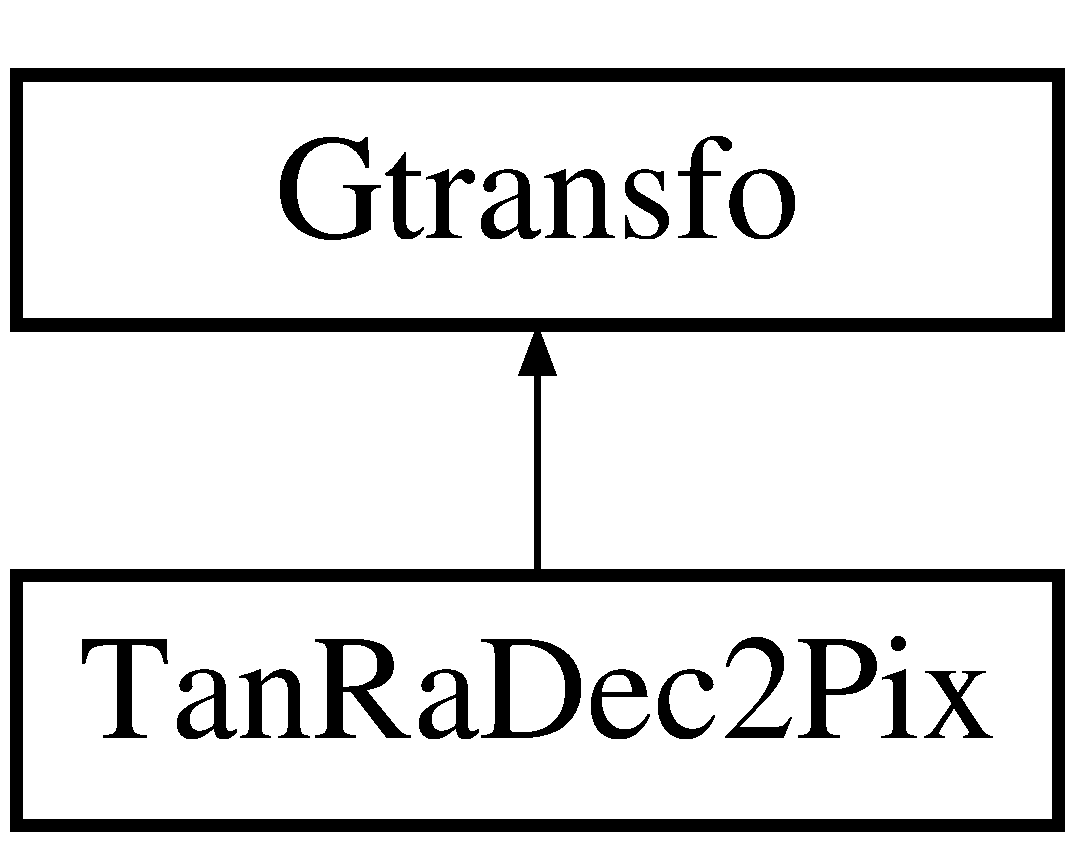
\includegraphics[height=2cm]{class_tanradec2pix}
\end{center}
\end{figure}
\subsubsection*{Public Methods}
\begin{CompactItemize}
\item 
\index{TanRaDec2Pix@{TanRaDec2Pix}!TanRaDec2Pix@{Tan\-Ra\-Dec2Pix}}\index{TanRaDec2Pix@{TanRaDec2Pix}!TanRaDec2Pix@{Tan\-Ra\-Dec2Pix}}
{\bf Tan\-Ra\-Dec2Pix} (const {\bf Gtransfo\-Lin} \&Tan2Pix, const {\bf Point} \&Tangent\-Point)\label{class_tanradec2pix_a0}

\begin{CompactList}\small\item\em assume degrees everywhere.\item\end{CompactList}\item 
\index{TanRaDec2Pix@{TanRaDec2Pix}!TanRaDec2Pix@{Tan\-Ra\-Dec2Pix}}\index{TanRaDec2Pix@{TanRaDec2Pix}!TanRaDec2Pix@{Tan\-Ra\-Dec2Pix}}
{\bf Tan\-Ra\-Dec2Pix} ()\label{class_tanradec2pix_a1}

\item 
\index{LinPart@{LinPart}!TanRaDec2Pix@{Tan\-Ra\-Dec2Pix}}\index{TanRaDec2Pix@{TanRaDec2Pix}!LinPart@{Lin\-Part}}
{\bf Gtransfo\-Lin} {\bf Lin\-Part} () const\label{class_tanradec2pix_a2}

\begin{CompactList}\small\item\em The Linear part (corresponding to CD's and CRPIX's).\item\end{CompactList}\item 
\index{TangentPoint@{TangentPoint}!TanRaDec2Pix@{Tan\-Ra\-Dec2Pix}}\index{TanRaDec2Pix@{TanRaDec2Pix}!TangentPoint@{Tangent\-Point}}
{\bf Point} {\bf Tangent\-Point} () const\label{class_tanradec2pix_a3}

\begin{CompactList}\small\item\em tangent point coordinates (in degrees).\item\end{CompactList}\item 
\index{apply@{apply}!TanRaDec2Pix@{Tan\-Ra\-Dec2Pix}}\index{TanRaDec2Pix@{TanRaDec2Pix}!apply@{apply}}
void {\bf apply} (const double Xin, const double Yin, double \&Yout, double \&Yout) const\label{class_tanradec2pix_a4}

\item 
\index{invert@{invert}!TanRaDec2Pix@{Tan\-Ra\-Dec2Pix}}\index{TanRaDec2Pix@{TanRaDec2Pix}!invert@{invert}}
{\bf Tan\-Pix2Ra\-Dec} {\bf invert} () const\label{class_tanradec2pix_a5}

\begin{CompactList}\small\item\em exact typed inverse:.\item\end{CompactList}\item 
\index{RoughInverse@{RoughInverse}!TanRaDec2Pix@{Tan\-Ra\-Dec2Pix}}\index{TanRaDec2Pix@{TanRaDec2Pix}!RoughInverse@{Rough\-Inverse}}
{\bf Gtransfo}$\ast$ {\bf Rough\-Inverse} (const {\bf Frame} \&Region) const\label{class_tanradec2pix_a6}

\begin{CompactList}\small\item\em Overload the \char`\"{}generic routine\char`\"{} (available for all {\bf Gtransfo} {\rm (p.\,\pageref{class_gtransfo})} types.\item\end{CompactList}\item 
\index{InverseTransfo@{InverseTransfo}!TanRaDec2Pix@{Tan\-Ra\-Dec2Pix}}\index{TanRaDec2Pix@{TanRaDec2Pix}!InverseTransfo@{Inverse\-Transfo}}
{\bf Gtransfo}$\ast$ {\bf Inverse\-Transfo} (const double Precision, const {\bf Frame} \&Region) const\label{class_tanradec2pix_a7}

\begin{CompactList}\small\item\em Inverse transfo: returns a {\bf Tan\-Pix2Ra\-Dec} {\rm (p.\,\pageref{class_tanpix2radec})}.\item\end{CompactList}\item 
\index{dump@{dump}!TanRaDec2Pix@{Tan\-Ra\-Dec2Pix}}\index{TanRaDec2Pix@{TanRaDec2Pix}!dump@{dump}}
void {\bf dump} (ostream \&stream) const\label{class_tanradec2pix_a8}

\begin{CompactList}\small\item\em dumps the transfo coefficients to stream.\item\end{CompactList}\item 
\index{Clone@{Clone}!TanRaDec2Pix@{Tan\-Ra\-Dec2Pix}}\index{TanRaDec2Pix@{TanRaDec2Pix}!Clone@{Clone}}
{\bf Gtransfo}$\ast$ {\bf Clone} () const\label{class_tanradec2pix_a9}

\begin{CompactList}\small\item\em returns a copy (allocated by new) of the transformation.\item\end{CompactList}\item 
double {\bf fit} (const Star\-Match\-List \&List, const {\bf Gtransfo} $\ast$Prior\-Transfo=NULL, const {\bf Gtransfo} $\ast$Posterior\-Transfo=NULL)
\begin{CompactList}\small\item\em fits a transfo to a list of star pairs (p1,p2).\item\end{CompactList}\end{CompactItemize}


\subsubsection{Detailed Description}
This one is the Tangent Plane (called gnomonic) projection (from celestial sphere to tangent plane).

this transfo does not implement corrections, since  they are defined the other way around (from pixels to sky),  and not invertible analytically. The inversion of tangent point WCS ({\bf Tan\-Pix2Ra\-Dec} {\rm (p.\,\pageref{class_tanpix2radec})}) is obtained via {\bf Inverse\-Transfo}() {\rm (p.\,\pageref{class_tanradec2pix_a7})}. 



\subsubsection{Member Function Documentation}
\index{TanRaDec2Pix@{Tan\-Ra\-Dec2Pix}!fit@{fit}}
\index{fit@{fit}!TanRaDec2Pix@{Tan\-Ra\-Dec2Pix}}
\paragraph{\setlength{\rightskip}{0pt plus 5cm}double Tan\-Ra\-Dec2Pix::fit (const Star\-Match\-List \& {\em List}, const {\bf Gtransfo} $\ast$ {\em Prior\-Transfo} = NULL, const {\bf Gtransfo} $\ast$ {\em Posterior\-Transfo} = NULL)\hspace{0.3cm}{\tt  [virtual]}}\hfill\label{class_tanradec2pix_a10}


fits a transfo to a list of star pairs (p1,p2).

After the fit this(Prior\-Transfo(p1)) yields approximately Posterior\-Transfo(p2). The returned value is the chi2. 

Reimplemented from {\bf Gtransfo} {\rm (p.\,\pageref{class_gtransfo_a4})}.

The documentation for this class was generated from the following file:\begin{CompactItemize}
\item 
{\bf gtransfo.h}\end{CompactItemize}

\subsection{Transformed\-Image  Class Reference}
\label{class_transformedimage}\index{TransformedImage@{Transformed\-Image}}
class that operates the transformation of a {\bf Reduced\-Image} {\rm (p.\,\pageref{class_reducedimage})} (image(s) + list). 


{\tt \#include $<$transformedimage.h$>$}

Inheritance diagram for Transformed\-Image::\begin{figure}[H]
\begin{center}
\leavevmode
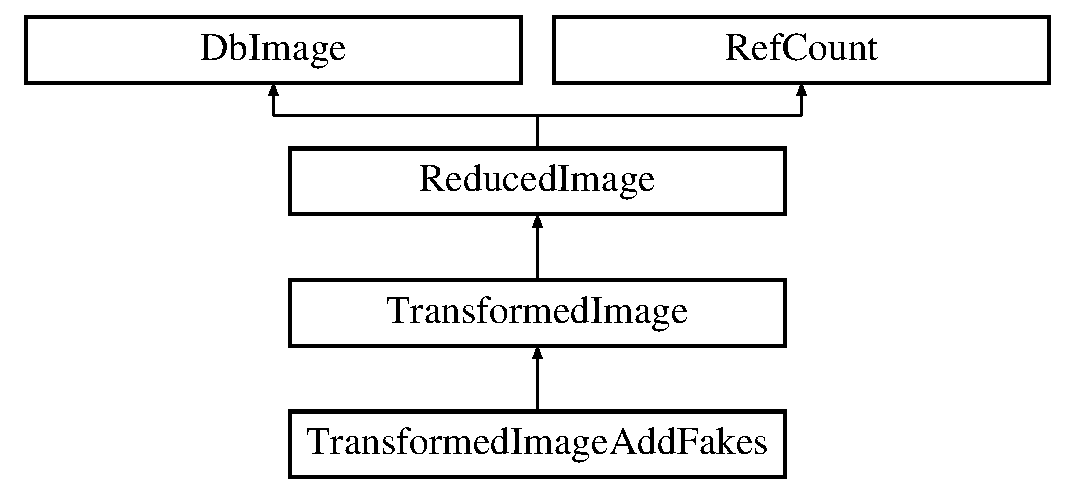
\includegraphics[height=4cm]{class_transformedimage}
\end{center}
\end{figure}
\subsubsection*{Public Methods}
\begin{CompactItemize}
\item 
{\bf Transformed\-Image} (const string \&Name, const {\bf Reduced\-Image} \&Source, const Image\-Transfo $\ast$Transfo)
\begin{CompactList}\small\item\em to create a new Transformed\-Image, or locate an existing one.\item\end{CompactList}\item 
\index{TransformedImage@{TransformedImage}!TransformedImage@{Transformed\-Image}}\index{TransformedImage@{TransformedImage}!TransformedImage@{Transformed\-Image}}
{\bf Transformed\-Image} (const string \&Name)\label{class_transformedimage_a1}

\begin{CompactList}\small\item\em assumes that the Transformed\-Image already exists.\item\end{CompactList}\item 
\index{TransformedImage@{TransformedImage}!TransformedImage@{Transformed\-Image}}\index{TransformedImage@{TransformedImage}!TransformedImage@{Transformed\-Image}}
{\bf Transformed\-Image} ()\label{class_transformedimage_a2}

\item 
\index{SourceName@{SourceName}!TransformedImage@{Transformed\-Image}}\index{TransformedImage@{TransformedImage}!SourceName@{Source\-Name}}
string {\bf Source\-Name} () const\label{class_transformedimage_a3}

\begin{CompactList}\small\item\em Original (untransformed) image name.\item\end{CompactList}\item 
\index{Source@{Source}!TransformedImage@{Transformed\-Image}}\index{TransformedImage@{TransformedImage}!Source@{Source}}
{\bf Reduced\-Image}$\ast$ {\bf Source} () const\label{class_transformedimage_a4}

\begin{CompactList}\small\item\em Original (untransformed) image.\item\end{CompactList}\item 
\index{GeometricReference@{GeometricReference}!TransformedImage@{Transformed\-Image}}\index{TransformedImage@{TransformedImage}!GeometricReference@{Geometric\-Reference}}
{\bf Reduced\-Image}$\ast$ {\bf Geometric\-Reference} ()\label{class_transformedimage_a5}

\begin{CompactList}\small\item\em Geometric reference (only applicable if Image\-Transfo is {\bf Image\-Gtransfo} {\rm (p.\,\pageref{class_imagegtransfo})}).\item\end{CompactList}\item 
\index{Transfo@{Transfo}!TransformedImage@{Transformed\-Image}}\index{TransformedImage@{TransformedImage}!Transfo@{Transfo}}
const Image\-Transfo$\ast$ {\bf Transfo} () const\label{class_transformedimage_a6}

\begin{CompactList}\small\item\em involved transformation.\item\end{CompactList}\item 
\index{FromRef@{FromRef}!TransformedImage@{Transformed\-Image}}\index{TransformedImage@{TransformedImage}!FromRef@{From\-Ref}}
const {\bf Gtransfo}$\ast$ {\bf From\-Ref} () const\label{class_transformedimage_a7}

\begin{CompactList}\small\item\em {\bf Gtransfo} {\rm (p.\,\pageref{class_gtransfo})} from reference to transformed image. Assumes that Image\-Transfo is an {\bf Image\-Gtransfo} {\rm (p.\,\pageref{class_imagegtransfo})}.\item\end{CompactList}\item 
\index{dump@{dump}!TransformedImage@{Transformed\-Image}}\index{TransformedImage@{TransformedImage}!dump@{dump}}
virtual void {\bf dump} (ostream \&s=cout) const\label{class_transformedimage_a8}

\begin{CompactList}\small\item\em dumps basic info.\item\end{CompactList}\item 
\index{MakeFits@{MakeFits}!TransformedImage@{Transformed\-Image}}\index{TransformedImage@{TransformedImage}!MakeFits@{Make\-Fits}}
virtual bool {\bf Make\-Fits} ()\label{class_transformedimage_a9}

\begin{CompactList}\small\item\em produce fits image.\item\end{CompactList}\item 
\index{MakeCatalog@{MakeCatalog}!TransformedImage@{Transformed\-Image}}\index{TransformedImage@{TransformedImage}!MakeCatalog@{Make\-Catalog}}
virtual bool {\bf Make\-Catalog} ()\label{class_transformedimage_a10}

\begin{CompactList}\small\item\em Produce the Saturated stars pixels mask, subtract the image background, detect with the SExtractor computed sigma. search the cosmics, and update catalog and weight for cosmics. No free coffee.\item\end{CompactList}\item 
\index{MakeDead@{MakeDead}!TransformedImage@{Transformed\-Image}}\index{TransformedImage@{TransformedImage}!MakeDead@{Make\-Dead}}
virtual bool {\bf Make\-Dead} ()\label{class_transformedimage_a11}

\begin{CompactList}\small\item\em produce dead image.\item\end{CompactList}\item 
\index{MakeSatur@{MakeSatur}!TransformedImage@{Transformed\-Image}}\index{TransformedImage@{TransformedImage}!MakeSatur@{Make\-Satur}}
virtual bool {\bf Make\-Satur} ()\label{class_transformedimage_a12}

\begin{CompactList}\small\item\em produce satur image.\item\end{CompactList}\item 
\index{MakeCosmic@{MakeCosmic}!TransformedImage@{Transformed\-Image}}\index{TransformedImage@{TransformedImage}!MakeCosmic@{Make\-Cosmic}}
virtual bool {\bf Make\-Cosmic} ()\label{class_transformedimage_a13}

\begin{CompactList}\small\item\em produce cosmic image.\item\end{CompactList}\item 
\index{MakeSatellite@{MakeSatellite}!TransformedImage@{Transformed\-Image}}\index{TransformedImage@{TransformedImage}!MakeSatellite@{Make\-Satellite}}
virtual bool {\bf Make\-Satellite} ()\label{class_transformedimage_a14}

\begin{CompactList}\small\item\em produce satellite image.\item\end{CompactList}\item 
\index{MakeWeight@{MakeWeight}!TransformedImage@{Transformed\-Image}}\index{TransformedImage@{TransformedImage}!MakeWeight@{Make\-Weight}}
virtual bool {\bf Make\-Weight} ()\label{class_transformedimage_a15}

\item 
\index{Create@{Create}!TransformedImage@{Transformed\-Image}}\index{TransformedImage@{TransformedImage}!Create@{Create}}
bool {\bf Create} (const string \&Where)\label{class_transformedimage_a16}

\begin{CompactList}\small\item\em To create the directories where the fits images, catalogues will be put: ex: $\sim$/Fake\-Db/test: {\bf Db\-Image} {\rm (p.\,\pageref{class_dbimage})} dbim(\char`\"{}test\char`\"{}); dbim.Create(\char`\"{}$\sim$/Fake\-Db/\char`\"{});.\item\end{CompactList}\item 
\index{Clone@{Clone}!TransformedImage@{Transformed\-Image}}\index{TransformedImage@{TransformedImage}!Clone@{Clone}}
{\bf Reduced\-Image}$\ast$ {\bf Clone} () const\label{class_transformedimage_a17}

\item 
\index{TransformedImage@{TransformedImage}!TransformedImage@{Transformed\-Image}}\index{TransformedImage@{TransformedImage}!TransformedImage@{Transformed\-Image}}
{\bf Transformed\-Image} (const Transformed\-Image \&Original)\label{class_transformedimage_a18}

\item 
\index{~TransformedImage@{$\sim$TransformedImage}!TransformedImage@{Transformed\-Image}}\index{TransformedImage@{TransformedImage}!~TransformedImage@{$\sim$Transformed\-Image}}
{\bf $\sim$Transformed\-Image} ()\label{class_transformedimage_a19}

\end{CompactItemize}


\subsubsection{Detailed Description}
class that operates the transformation of a {\bf Reduced\-Image} {\rm (p.\,\pageref{class_reducedimage})} (image(s) + list).

As for other descendants of {\bf Reduced\-Image} {\rm (p.\,\pageref{class_reducedimage})}, the actual computations occur when you request the name of a data file (e.g. {\bf Fits\-Name}() {\rm (p.\,\pageref{class_reducedimage_a14})}). To geometrically align a set of images on the same reference, use Images\-Align(). If you want to sum them, uses Images\-Align\-And\-Sum() 



\subsubsection{Constructor \& Destructor Documentation}
\index{TransformedImage@{Transformed\-Image}!TransformedImage@{TransformedImage}}
\index{TransformedImage@{TransformedImage}!TransformedImage@{Transformed\-Image}}
\paragraph{\setlength{\rightskip}{0pt plus 5cm}Transformed\-Image::Transformed\-Image (const string \& {\em Name}, const {\bf Reduced\-Image} \& {\em Source}, const Image\-Transfo $\ast$ {\em Transfo})}\hfill\label{class_transformedimage_a0}


to create a new Transformed\-Image, or locate an existing one.

If you want to align A on B, the typical constructor call will be: Transformed\-Image(New\-Name, A, \&Image\-Gtransfo(B,A)); To align a set of images on the same reference, use Images\-Align(). 

The documentation for this class was generated from the following file:\begin{CompactItemize}
\item 
{\bf transformedimage.h}\end{CompactItemize}

\subsection{Vignet  Class Reference}
\label{class_vignet}\index{Vignet@{Vignet}}
Similar to {\bf Kernel} {\rm (p.\,\pageref{class_kernel})}, but resizeable and contains some kind of {\bf Point} {\rm (p.\,\pageref{class_point})}. 


{\tt \#include $<$vignet.h$>$}

Inheritance diagram for Vignet::\begin{figure}[H]
\begin{center}
\leavevmode
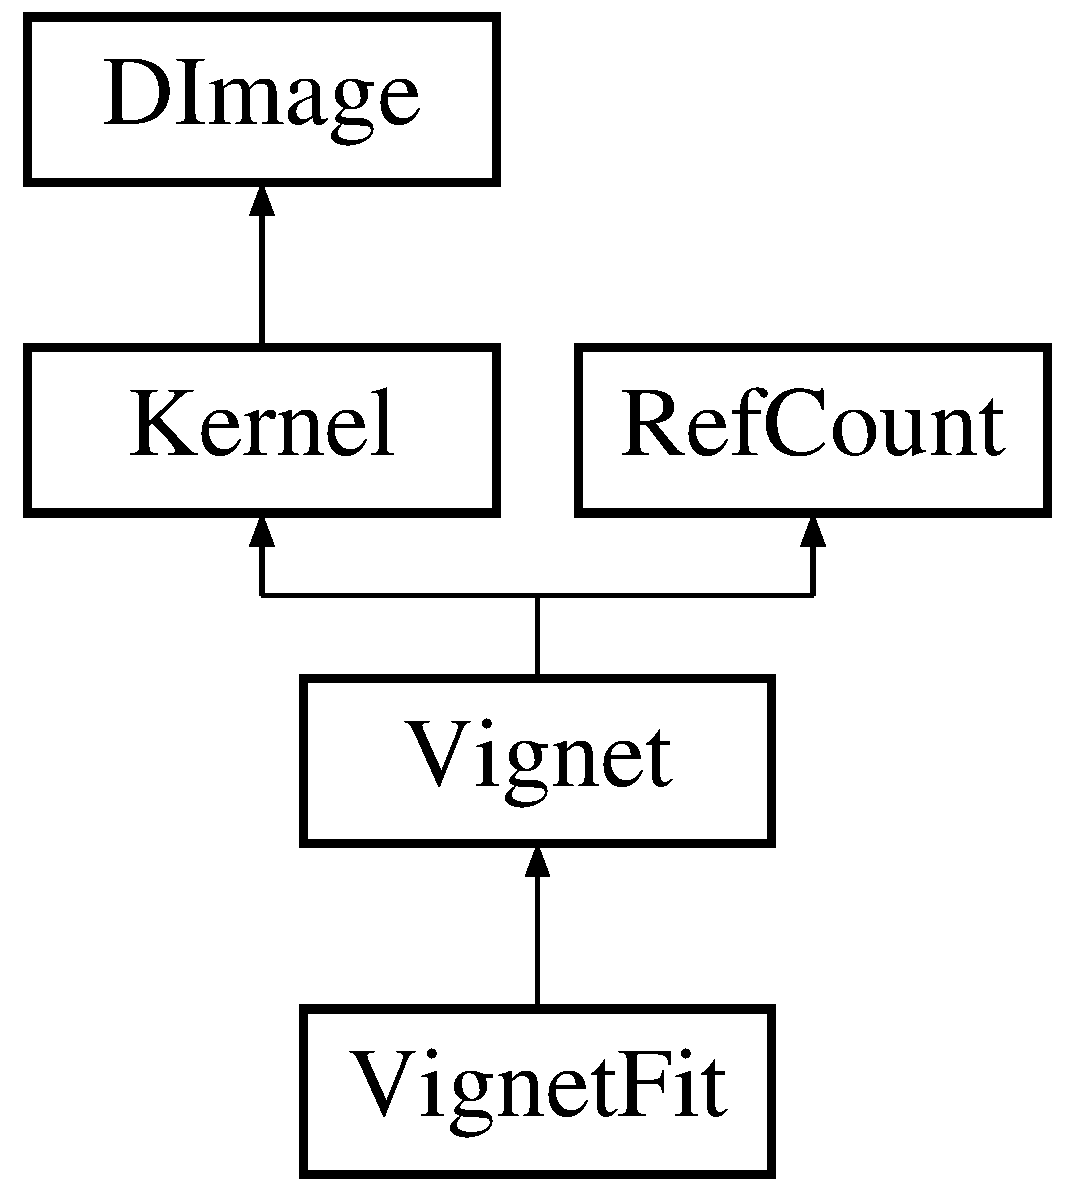
\includegraphics[height=4cm]{class_vignet}
\end{center}
\end{figure}
\subsubsection*{Public Methods}
\begin{CompactItemize}
\item 
\index{Vignet@{Vignet}!Vignet@{Vignet}}\index{Vignet@{Vignet}!Vignet@{Vignet}}
{\bf Vignet} (const double \&X, const double \&Y, const {\bf Image} \&Source, const int HMax\-X, const int HMax\-Y)\label{class_vignet_a0}

\item 
\index{Vignet@{Vignet}!Vignet@{Vignet}}\index{Vignet@{Vignet}!Vignet@{Vignet}}
{\bf Vignet} (const double \&X, const double \&Y, const int HMax\-X, const int HMax\-Y)\label{class_vignet_a1}

\item 
\index{Vignet@{Vignet}!Vignet@{Vignet}}\index{Vignet@{Vignet}!Vignet@{Vignet}}
{\bf Vignet} (const string \&File\-Name)\label{class_vignet_a2}

\item 
\index{Vignet@{Vignet}!Vignet@{Vignet}}\index{Vignet@{Vignet}!Vignet@{Vignet}}
{\bf Vignet} ()\label{class_vignet_a3}

\item 
\index{~Vignet@{$\sim$Vignet}!Vignet@{Vignet}}\index{Vignet@{Vignet}!~Vignet@{$\sim$Vignet}}
{\bf $\sim$Vignet} ()\label{class_vignet_a4}

\item 
\index{Resize@{Resize}!Vignet@{Vignet}}\index{Vignet@{Vignet}!Resize@{Resize}}
void {\bf Resize} (const int HSize\-X, const int HSize\-Y)\label{class_vignet_a5}

\item 
\index{Resize@{Resize}!Vignet@{Vignet}}\index{Vignet@{Vignet}!Resize@{Resize}}
void {\bf Resize} (const double \&Scale\-Factor)\label{class_vignet_a6}

\item 
\index{Detect@{Detect}!Vignet@{Vignet}}\index{Vignet@{Vignet}!Detect@{Detect}}
void {\bf Detect} (const double \&Pos\-Thresh, const double \&Neg\-Thresh)\label{class_vignet_a7}

\item 
\index{Aperture@{Aperture}!Vignet@{Vignet}}\index{Vignet@{Vignet}!Aperture@{Aperture}}
double {\bf Aperture} (double \&Var\-Aper, const double \&Radius, const double \&Var\-Pix, const double \&Sky) const\label{class_vignet_a8}

\item 
\index{WeightedAperture@{WeightedAperture}!Vignet@{Vignet}}\index{Vignet@{Vignet}!WeightedAperture@{Weighted\-Aperture}}
double {\bf Weighted\-Aperture} (double \&Var\-Aper, const {\bf Kernel} \&Model, const double \&Var\-Pix, const double \&Sky) const\label{class_vignet_a9}

\item 
\index{WeightedRecentroid@{WeightedRecentroid}!Vignet@{Vignet}}\index{Vignet@{Vignet}!WeightedRecentroid@{Weighted\-Recentroid}}
void {\bf Weighted\-Recentroid} (double \&Flux, const double \&Sky, const double \&Sig\-X, const double \&Sigy)\label{class_vignet_a10}

\item 
\index{Hx@{Hx}!Vignet@{Vignet}}\index{Vignet@{Vignet}!Hx@{Hx}}
int {\bf Hx} () const\label{class_vignet_a11}

\item 
\index{Hy@{Hy}!Vignet@{Vignet}}\index{Vignet@{Vignet}!Hy@{Hy}}
int {\bf Hy} () const\label{class_vignet_a12}

\item 
\index{readFits@{readFits}!Vignet@{Vignet}}\index{Vignet@{Vignet}!readFits@{read\-Fits}}
void {\bf read\-Fits} (const string \&File\-Name)\label{class_vignet_a13}

\begin{CompactList}\small\item\em write and read the {\bf DImage} {\rm (p.\,\pageref{class_dimage})} as a FITS array.\item\end{CompactList}\item 
\index{writeFits@{writeFits}!Vignet@{Vignet}}\index{Vignet@{Vignet}!writeFits@{write\-Fits}}
void {\bf write\-Fits} (const string \&File\-Name) const\label{class_vignet_a14}

\end{CompactItemize}
\subsubsection*{Public Attributes}
\begin{CompactItemize}
\item 
\index{ic@{ic}!Vignet@{Vignet}}\index{Vignet@{Vignet}!ic@{ic}}
int {\bf ic}\label{class_vignet_m0}

\begin{CompactList}\small\item\em coordinates of the center pixel where the Vignet was grabbed from.\item\end{CompactList}\item 
\index{jc@{jc}!Vignet@{Vignet}}\index{Vignet@{Vignet}!jc@{jc}}
int {\bf jc}\label{class_vignet_m1}

\begin{CompactList}\small\item\em coordinates of the center pixel where the Vignet was grabbed from.\item\end{CompactList}\item 
\index{dxc@{dxc}!Vignet@{Vignet}}\index{Vignet@{Vignet}!dxc@{dxc}}
double {\bf dxc}\label{class_vignet_m2}

\begin{CompactList}\small\item\em real coordinates of the star centroid relative to the down-left corner of center pixel (ic,jc).\item\end{CompactList}\item 
\index{dyc@{dyc}!Vignet@{Vignet}}\index{Vignet@{Vignet}!dyc@{dyc}}
double {\bf dyc}\label{class_vignet_m3}

\begin{CompactList}\small\item\em real coordinates of the star centroid relative to the down-left corner of center pixel (ic,jc).\item\end{CompactList}\item 
\index{istart@{istart}!Vignet@{Vignet}}\index{Vignet@{Vignet}!istart@{istart}}
int {\bf istart}\label{class_vignet_m4}

\begin{CompactList}\small\item\em image coordinates of the down-left corner pixel where the Vignet was grabbed.\item\end{CompactList}\item 
\index{jstart@{jstart}!Vignet@{Vignet}}\index{Vignet@{Vignet}!jstart@{jstart}}
int {\bf jstart}\label{class_vignet_m5}

\begin{CompactList}\small\item\em image coordinates of the down-left corner pixel where the Vignet was grabbed.\item\end{CompactList}\item 
\index{iend@{iend}!Vignet@{Vignet}}\index{Vignet@{Vignet}!iend@{iend}}
int {\bf iend}\label{class_vignet_m6}

\begin{CompactList}\small\item\em image coordinates of the upper-right corner pixel where the Vignet was grabbed.\item\end{CompactList}\item 
\index{jend@{jend}!Vignet@{Vignet}}\index{Vignet@{Vignet}!jend@{jend}}
int {\bf jend}\label{class_vignet_m7}

\begin{CompactList}\small\item\em image coordinates of the upper-right corner pixel where the Vignet was grabbed.\item\end{CompactList}\end{CompactItemize}
\subsubsection*{Protected Attributes}
\begin{CompactItemize}
\item 
\index{hx@{hx}!Vignet@{Vignet}}\index{Vignet@{Vignet}!hx@{hx}}
int {\bf hx}\label{class_vignet_n0}

\item 
\index{hy@{hy}!Vignet@{Vignet}}\index{Vignet@{Vignet}!hy@{hy}}
int {\bf hy}\label{class_vignet_n1}

\end{CompactItemize}


\subsubsection{Detailed Description}
Similar to {\bf Kernel} {\rm (p.\,\pageref{class_kernel})}, but resizeable and contains some kind of {\bf Point} {\rm (p.\,\pageref{class_point})}.



The documentation for this class was generated from the following file:\begin{CompactItemize}
\item 
{\bf vignet.h}\end{CompactItemize}

\section{toads File Documentation}
\subsection{allreducedimage.h File Reference}
\label{allreducedimage_h}\index{allreducedimage.h@{allreducedimage.h}}
utilities around all derived classes ot {\bf Reduced\-Image} {\rm (p.\,\pageref{class_reducedimage})}. 


{\tt \#include $<$string$>$}\par
\subsubsection*{Namespaces}
\begin{CompactItemize}
\item 
namespace {\bf std}
\end{CompactItemize}
\subsubsection*{Functions}
\begin{CompactItemize}
\item 
\index{ReducedImageNew@{ReducedImageNew}!allreducedimage.h@{allreducedimage.h}}\index{allreducedimage.h@{allreducedimage.h}!ReducedImageNew@{Reduced\-Image\-New}}
{\bf Reduced\-Image}$\ast$ {\bf Reduced\-Image\-New} (const string \&Name)\label{allreducedimage_h_a0}

\begin{CompactList}\small\item\em 'virtual' constructor. Not totally functionnal unfortunately.\item\end{CompactList}\item 
\index{IsTransformedImage@{IsTransformedImage}!allreducedimage.h@{allreducedimage.h}}\index{allreducedimage.h@{allreducedimage.h}!IsTransformedImage@{Is\-Transformed\-Image}}
const {\bf Transformed\-Image}$\ast$ {\bf Is\-Transformed\-Image} (const {\bf Reduced\-Image} $\ast$RImage)\label{allreducedimage_h_a1}

\begin{CompactList}\small\item\em returns NULL if the argument is not a {\bf Transformed\-Image} {\rm (p.\,\pageref{class_transformedimage})}.\item\end{CompactList}\item 
\index{IsTransformedImage@{IsTransformedImage}!allreducedimage.h@{allreducedimage.h}}\index{allreducedimage.h@{allreducedimage.h}!IsTransformedImage@{Is\-Transformed\-Image}}
{\bf Transformed\-Image}$\ast$ {\bf Is\-Transformed\-Image} ({\bf Reduced\-Image} $\ast$RImage)\label{allreducedimage_h_a2}

\item 
\index{IsImageSum@{IsImageSum}!allreducedimage.h@{allreducedimage.h}}\index{allreducedimage.h@{allreducedimage.h}!IsImageSum@{Is\-Image\-Sum}}
const {\bf Image\-Sum}$\ast$ {\bf Is\-Image\-Sum} (const {\bf Reduced\-Image} $\ast$RImage)\label{allreducedimage_h_a3}

\begin{CompactList}\small\item\em returns NULL if the argument is not an {\bf Image\-Sum} {\rm (p.\,\pageref{class_imagesum})}.\item\end{CompactList}\item 
\index{IsImageSum@{IsImageSum}!allreducedimage.h@{allreducedimage.h}}\index{allreducedimage.h@{allreducedimage.h}!IsImageSum@{Is\-Image\-Sum}}
{\bf Image\-Sum}$\ast$ {\bf Is\-Image\-Sum} ({\bf Reduced\-Image} $\ast$RImage)\label{allreducedimage_h_a4}

\end{CompactItemize}


\subsubsection{Detailed Description}
utilities around all derived classes ot {\bf Reduced\-Image} {\rm (p.\,\pageref{class_reducedimage})}.




\subsection{astroutils.h File Reference}
\label{astroutils_h}\index{astroutils.h@{astroutils.h}}
{\tt \#include $<$string$>$}\par
\subsubsection*{Functions}
\begin{CompactItemize}
\item 
\index{IsLeapYear@{IsLeapYear}!astroutils.h@{astroutils.h}}\index{astroutils.h@{astroutils.h}!IsLeapYear@{Is\-Leap\-Year}}
bool {\bf Is\-Leap\-Year} (const int year)\label{astroutils_h_a0}

\item 
\index{JulianDay@{JulianDay}!astroutils.h@{astroutils.h}}\index{astroutils.h@{astroutils.h}!JulianDay@{Julian\-Day}}
long {\bf Julian\-Day} (const int day, const int month, const int year)\label{astroutils_h_a1}

\item 
\index{JulianDay@{JulianDay}!astroutils.h@{astroutils.h}}\index{astroutils.h@{astroutils.h}!JulianDay@{Julian\-Day}}
double {\bf Julian\-Day} (const int day, const int month, const int year, const int hour, const int min, const double sec)\label{astroutils_h_a2}

\item 
\index{JulianDay@{JulianDay}!astroutils.h@{astroutils.h}}\index{astroutils.h@{astroutils.h}!JulianDay@{Julian\-Day}}
double {\bf Julian\-Day} (const {\bf Fits\-Header} \&Header)\label{astroutils_h_a3}

\begin{CompactList}\small\item\em computes the julian date given a header.\item\end{CompactList}\item 
\index{RedJulianDay@{RedJulianDay}!astroutils.h@{astroutils.h}}\index{astroutils.h@{astroutils.h}!RedJulianDay@{Red\-Julian\-Day}}
double {\bf Red\-Julian\-Day} (const {\bf Fits\-Header} \&Header)\label{astroutils_h_a4}

\begin{CompactList}\small\item\em computes the reduced julian date given a header.\item\end{CompactList}\item 
\index{UtStringToDeci@{UtStringToDeci}!astroutils.h@{astroutils.h}}\index{astroutils.h@{astroutils.h}!UtStringToDeci@{Ut\-String\-To\-Deci}}
double {\bf Ut\-String\-To\-Deci} (const string Ut\-String)\label{astroutils_h_a5}

\item 
\index{RaStringToDeg@{RaStringToDeg}!astroutils.h@{astroutils.h}}\index{astroutils.h@{astroutils.h}!RaStringToDeg@{Ra\-String\-To\-Deg}}
double {\bf Ra\-String\-To\-Deg} (const string Ra\-String)\label{astroutils_h_a6}

\begin{CompactList}\small\item\em -.\item\end{CompactList}\item 
\index{DecStringToDeg@{DecStringToDeg}!astroutils.h@{astroutils.h}}\index{astroutils.h@{astroutils.h}!DecStringToDeg@{Dec\-String\-To\-Deg}}
double {\bf Dec\-String\-To\-Deg} (const string Dec\-String)\label{astroutils_h_a7}

\begin{CompactList}\small\item\em -.\item\end{CompactList}\item 
\index{UtDeciToString@{UtDeciToString}!astroutils.h@{astroutils.h}}\index{astroutils.h@{astroutils.h}!UtDeciToString@{Ut\-Deci\-To\-String}}
string {\bf Ut\-Deci\-To\-String} (double Ut\-Deci)\label{astroutils_h_a8}

\begin{CompactList}\small\item\em -.\item\end{CompactList}\item 
\index{RaDegToString@{RaDegToString}!astroutils.h@{astroutils.h}}\index{astroutils.h@{astroutils.h}!RaDegToString@{Ra\-Deg\-To\-String}}
string {\bf Ra\-Deg\-To\-String} (double Ra\-Deg)\label{astroutils_h_a9}

\item 
\index{DecDegToString@{DecDegToString}!astroutils.h@{astroutils.h}}\index{astroutils.h@{astroutils.h}!DecDegToString@{Dec\-Deg\-To\-String}}
string {\bf Dec\-Deg\-To\-String} (double Dec\-Deg)\label{astroutils_h_a10}

\begin{CompactList}\small\item\em -.\item\end{CompactList}\item 
\index{GetRaDecInDeg@{GetRaDecInDeg}!astroutils.h@{astroutils.h}}\index{astroutils.h@{astroutils.h}!GetRaDecInDeg@{Get\-Ra\-Dec\-In\-Deg}}
void {\bf Get\-Ra\-Dec\-In\-Deg} ({\bf Fits\-Header} const \&Header, double \&Ra\-In\-Deg, double \&Dec\-In\-Deg)\label{astroutils_h_a11}

\begin{CompactList}\small\item\em -.\item\end{CompactList}\item 
\index{RaDec2000@{RaDec2000}!astroutils.h@{astroutils.h}}\index{astroutils.h@{astroutils.h}!RaDec2000@{Ra\-Dec2000}}
void {\bf Ra\-Dec2000} ({\bf Fits\-Header} const \&Header, double \&Ra\-In\-Deg, double \&Dec\-In\-Deg)\label{astroutils_h_a12}

\begin{CompactList}\small\item\em returns alpha delta in 2000 whatever the equinox used in header.\item\end{CompactList}\end{CompactItemize}


\subsubsection{Detailed Description}



\subsection{basestar.h File Reference}
\label{basestar_h}\index{basestar.h@{basestar.h}}
{\tt \#include $<$iostream$>$}\par
{\tt \#include $<$cstdio$>$}\par
{\tt \#include $<$string$>$}\par
{\tt \#include \char`\"{}point.h\char`\"{}}\par
{\tt \#include \char`\"{}countedref.h\char`\"{}}\par
{\tt \#include \char`\"{}rootstuff.h\char`\"{}}\par
{\tt \#include \char`\"{}starlist.h\char`\"{}}\par
\subsubsection*{Compounds}
\begin{CompactItemize}
\item 
class {\bf Base\-Star}
\begin{CompactList}\small\item\em The base class for handling stars. Used by all matching routines.\item\end{CompactList}\end{CompactItemize}
\subsubsection*{Defines}
\begin{CompactItemize}
\item 
\index{MEMPIX2DISK@{MEMPIX2DISK}!basestar.h@{basestar.h}}\index{basestar.h@{basestar.h}!MEMPIX2DISK@{MEMPIX2DISK}}
\#define {\bf MEMPIX2DISK}\ 1\label{basestar_h_a0}

\item 
\index{DECALAGE_IJ_XY@{DECALAGE\_\-IJ\_\-XY}!basestar.h@{basestar.h}}\index{basestar.h@{basestar.h}!DECALAGE_IJ_XY@{DECALAGE\_\-IJ\_\-XY}}
\#define {\bf DECALAGE\_\-IJ\_\-XY}\ 0.\label{basestar_h_a1}

\item 
\index{DECALAGE_XY_IJ@{DECALAGE\_\-XY\_\-IJ}!basestar.h@{basestar.h}}\index{basestar.h@{basestar.h}!DECALAGE_XY_IJ@{DECALAGE\_\-XY\_\-IJ}}
\#define {\bf DECALAGE\_\-XY\_\-IJ}\ 0.\label{basestar_h_a2}

\end{CompactItemize}
\subsubsection*{Typedefs}
\begin{CompactItemize}
\item 
\index{BaseStarList@{BaseStarList}!basestar.h@{basestar.h}}\index{basestar.h@{basestar.h}!BaseStarList@{Base\-Star\-List}}
typedef {\bf Star\-List}$<${\bf Base\-Star}$>$ {\bf Base\-Star\-List}\label{basestar_h_a3}

\item 
\index{BaseStarCIterator@{BaseStarCIterator}!basestar.h@{basestar.h}}\index{basestar.h@{basestar.h}!BaseStarCIterator@{Base\-Star\-CIterator}}
typedef Base\-Star\-List::const\_\-iterator {\bf Base\-Star\-CIterator}\label{basestar_h_a4}

\item 
\index{BaseStarIterator@{BaseStarIterator}!basestar.h@{basestar.h}}\index{basestar.h@{basestar.h}!BaseStarIterator@{Base\-Star\-Iterator}}
typedef Base\-Star\-List::iterator {\bf Base\-Star\-Iterator}\label{basestar_h_a5}

\item 
\index{BaseStarRef@{BaseStarRef}!basestar.h@{basestar.h}}\index{basestar.h@{basestar.h}!BaseStarRef@{Base\-Star\-Ref}}
typedef {\bf Counted\-Ref}$<${\bf Base\-Star}$>$ {\bf Base\-Star\-Ref}\label{basestar_h_a6}

\end{CompactItemize}
\subsubsection*{Functions}
\begin{CompactItemize}
\item 
\index{DecreasingFlux@{DecreasingFlux}!basestar.h@{basestar.h}}\index{basestar.h@{basestar.h}!DecreasingFlux@{Decreasing\-Flux}}
bool {\bf Decreasing\-Flux} (const {\bf Base\-Star} $\ast$S1, const {\bf Base\-Star} $\ast$S2)\label{basestar_h_a7}

\begin{CompactList}\small\item\em enables to sort easily a star\-List (of anything that derives from {\bf Base\-Star} {\rm (p.\,\pageref{class_basestar})}).\item\end{CompactList}\item 
\index{DecodeFormat@{DecodeFormat}!basestar.h@{basestar.h}}\index{basestar.h@{basestar.h}!DecodeFormat@{Decode\-Format}}
int {\bf Decode\-Format} (const char $\ast$Format\-Line, const char $\ast$Star\-Name)\label{basestar_h_a8}

\end{CompactItemize}


\subsubsection{Detailed Description}



\subsection{dbimage.h File Reference}
\label{dbimage_h}\index{dbimage.h@{dbimage.h}}
documentation for the {\bf Db\-Image} {\rm (p.\,\pageref{class_dbimage})} class and the {\bf The data base configuration file.} {\rm (p.\,\pageref{dbconfig})} file, and more generally, the {\bf Data\-Base} {\rm (p.\,\pageref{database_page})}. 


{\tt \#include $<$string$>$}\par
{\tt \#include $<$iostream$>$}\par
{\tt \#include \char`\"{}rootstuff.h\char`\"{}}\par
{\tt \#include $<$list$>$}\par
\subsubsection*{Compounds}
\begin{CompactItemize}
\item 
class {\bf Db\-Image}
\item 
class {\bf Db\-Image\-List}
\begin{CompactList}\small\item\em Db\-Images can be globally located and stored into image lists.\item\end{CompactList}\end{CompactItemize}
\subsubsection*{Typedefs}
\begin{CompactItemize}
\item 
\index{DbImageIterator@{DbImageIterator}!dbimage.h@{dbimage.h}}\index{dbimage.h@{dbimage.h}!DbImageIterator@{Db\-Image\-Iterator}}
typedef list$<${\bf Db\-Image}$>$::iterator {\bf Db\-Image\-Iterator}\label{dbimage_h_a0}

\item 
\index{DbImageCIterator@{DbImageCIterator}!dbimage.h@{dbimage.h}}\index{dbimage.h@{dbimage.h}!DbImageCIterator@{Db\-Image\-CIterator}}
typedef list$<${\bf Db\-Image}$>$::const\_\-iterator {\bf Db\-Image\-CIterator}\label{dbimage_h_a1}

\end{CompactItemize}
\subsubsection*{Enumerations}
\begin{CompactItemize}
\item 
enum {\bf Db\-Image\-Kind} \{ {\bf Raw} =  1, 
{\bf Calibrated}, 
{\bf Elixir}
 \}
\item 
enum {\bf Db\-Image\-Catalog\-Kind} \{ {\bf SExtractor} =  1, 
{\bf Fitted\_\-for\_\-seeing}, 
{\bf Daophot\-Als}, 
{\bf Daophot\-Ap}, 
{\bf Daophot\-Nei}, 
{\bf Daophot\-Lst}, 
{\bf Daophot\-Pk}, 
{\bf Daophot\-Nst}
 \}
\item 
enum {\bf Db\-Image\-Psf\-Kind} \{ {\bf Daophot\-Psf} =  1
 \}
\end{CompactItemize}
\subsubsection*{Functions}
\begin{CompactItemize}
\item 
void {\bf Db\-Init} ()
\begin{CompactList}\small\item\em reads the config file. Called automatically if not user called.\item\end{CompactList}\item 
void {\bf Db\-Config\-Dump} (ostream \&stream=cout)
\begin{CompactList}\small\item\em dumps to cout the (interpreted) contents of the configuration file.\item\end{CompactList}\item 
\index{InstallImage@{InstallImage}!dbimage.h@{dbimage.h}}\index{dbimage.h@{dbimage.h}!InstallImage@{Install\-Image}}
int {\bf Install\-Image} (const char $\ast$a\_\-path, const char $\ast$a\_\-file, Db\-Image\-Kind kind)\label{dbimage_h_a16}

\item 
\index{AssignInfo@{AssignInfo}!dbimage.h@{dbimage.h}}\index{dbimage.h@{dbimage.h}!AssignInfo@{Assign\-Info}}
int {\bf Assign\-Info} (const {\bf Db\-Image} \&{\bf Image}, const string \&Flat\-Fits\-File\-Name, const char $\ast$Which\-Info)\label{dbimage_h_a17}

\item 
\index{DbConfigSetDumpLevel@{DbConfigSetDumpLevel}!dbimage.h@{dbimage.h}}\index{dbimage.h@{dbimage.h}!DbConfigSetDumpLevel@{Db\-Config\-Set\-Dump\-Level}}
int {\bf Db\-Config\-Set\-Dump\-Level} (const int level)\label{dbimage_h_a18}

\item 
\index{DbConfigFileName@{DbConfigFileName}!dbimage.h@{dbimage.h}}\index{dbimage.h@{dbimage.h}!DbConfigFileName@{Db\-Config\-File\-Name}}
string {\bf Db\-Config\-File\-Name} ()\label{dbimage_h_a19}

\item 
\index{DbConfigAddImagePath@{DbConfigAddImagePath}!dbimage.h@{dbimage.h}}\index{dbimage.h@{dbimage.h}!DbConfigAddImagePath@{Db\-Config\-Add\-Image\-Path}}
void {\bf Db\-Config\-Add\-Image\-Path} (const char $\ast$a\_\-path, const char $\ast$a\_\-path\_\-name)\label{dbimage_h_a20}

\item 
\index{DbConfigFileParse@{DbConfigFileParse}!dbimage.h@{dbimage.h}}\index{dbimage.h@{dbimage.h}!DbConfigFileParse@{Db\-Config\-File\-Parse}}
int {\bf Db\-Config\-File\-Parse} (const char $\ast$Config\-File\-Name)\label{dbimage_h_a21}

\end{CompactItemize}


\subsubsection{Detailed Description}
documentation for the {\bf Db\-Image} {\rm (p.\,\pageref{class_dbimage})} class and the {\bf The data base configuration file.} {\rm (p.\,\pageref{dbconfig})} file, and more generally, the {\bf Data\-Base} {\rm (p.\,\pageref{database_page})}.





\subsubsection{Function Documentation}
\index{dbimage.h@{dbimage.h}!DbConfigDump@{DbConfigDump}}
\index{DbConfigDump@{DbConfigDump}!dbimage.h@{dbimage.h}}
\paragraph{\setlength{\rightskip}{0pt plus 5cm}void Db\-Config\-Dump (ostream \& {\em stream} = cout)}\hfill\label{dbimage_h_a15}


dumps to cout the (interpreted) contents of the configuration file.

It triggers Db\-Init if not already done. \index{dbimage.h@{dbimage.h}!DbInit@{DbInit}}
\index{DbInit@{DbInit}!dbimage.h@{dbimage.h}}
\paragraph{\setlength{\rightskip}{0pt plus 5cm}void Db\-Init ()}\hfill\label{dbimage_h_a14}


reads the config file. Called automatically if not user called.

If you programm does a lot of things before actually calling any {\bf Db\-Image} {\rm (p.\,\pageref{class_dbimage})} constructor,  it may be a good idea to call it early in your main to check if the configuration file is correct. 
\subsection{fastfinder.h File Reference}
\label{fastfinder_h}\index{fastfinder.h@{fastfinder.h}}
Fast locator in starlists. 


{\tt \#include \char`\"{}basestar.h\char`\"{}}\par
\subsubsection*{Compounds}
\begin{CompactItemize}
\item 
class {\bf Fast\-Finder}
\begin{CompactList}\small\item\em Fast locator in starlists.\item\end{CompactList}\item 
class {\bf Fast\-Finder::Iterator}
\end{CompactItemize}


\subsubsection{Detailed Description}
Fast locator in starlists.




\subsection{fitsimage.h File Reference}
\label{fitsimage_h}\index{fitsimage.h@{fitsimage.h}}
I/O of images/headers in fits format. 


{\tt \#include $<$string$>$}\par
{\tt \#include $<$cstdio$>$}\par
{\tt \#include $<$cstring$>$}\par
{\tt \#include \char`\"{}image.h\char`\"{}}\par
{\tt \#include \char`\"{}point.h\char`\"{}}\par
{\tt \#include $<$fitsio.h$>$}\par
{\tt \#include $<$vector$>$}\par
\subsubsection*{Compounds}
\begin{CompactItemize}
\item 
class {\bf Fits\-Header}
\begin{CompactList}\small\item\em Fits files and header keys.\item\end{CompactList}\item 
class {\bf Fits\-Image}
\begin{CompactList}\small\item\em This class enables basic manipulation of images stored in fits files.\item\end{CompactList}\item 
class {\bf Fits\-Key}
\begin{CompactList}\small\item\em Auxilary class for accessing fits header keys.\item\end{CompactList}\item 
class {\bf Fits\-Key\-Array}
\end{CompactItemize}
\subsubsection*{Defines}
\begin{CompactItemize}
\item 
\index{NOVAL@{NOVAL}!fitsimage.h@{fitsimage.h}}\index{fitsimage.h@{fitsimage.h}!NOVAL@{NOVAL}}
\#define {\bf NOVAL}\ string(\char`\"{}NOVAL\char`\"{})\label{fitsimage_h_a0}

\end{CompactItemize}
\subsubsection*{Enumerations}
\begin{CompactItemize}
\item 
enum {\bf Fits\-File\-Mode} \{ {\bf RO} =  0, 
{\bf RW} =  1
 \}
\end{CompactItemize}


\subsubsection{Detailed Description}
I/O of images/headers in fits format.

The IO of images in the fits format are carried out using the cfitsio library. This library is written in C, and the most useful functionnalities have been wrapped here in C++ classes.


\subsection{fitsset.h File Reference}
\label{fitsset_h}\index{fitsset.h@{fitsset.h}}
sets of fits files with homogeneous sizes, filter, and chip id. 


{\tt \#include $<$string$>$}\par
{\tt \#include $<$vector$>$}\par
\subsubsection*{Compounds}
\begin{CompactItemize}
\item 
class {\bf Fits\-Set}
\begin{CompactList}\small\item\em container for fits files that have same sizes, filter, and come from the same chip within a mosaic.\item\end{CompactList}\end{CompactItemize}


\subsubsection{Detailed Description}
sets of fits files with homogeneous sizes, filter, and chip id.




\subsection{fitsslice.h File Reference}
\label{fitsslice_h}\index{fitsslice.h@{fitsslice.h}}
Load successively slices of fits images in memory. 


{\tt \#include $<$string$>$}\par
{\tt \#include \char`\"{}fitsimage.h\char`\"{}}\par
{\tt \#include $<$vector$>$}\par
\subsubsection*{Compounds}
\begin{CompactItemize}
\item 
class {\bf Fits\-Parallel\-Slices}
\begin{CompactList}\small\item\em Several fits images of the same size to be processed in parallel.\item\end{CompactList}\item 
class {\bf Fits\-Slice}
\begin{CompactList}\small\item\em Memory saving traversal of a fits image.\item\end{CompactList}\end{CompactItemize}
\subsubsection*{Typedefs}
\begin{CompactItemize}
\item 
\index{FitsSliceIterator@{FitsSliceIterator}!fitsslice.h@{fitsslice.h}}\index{fitsslice.h@{fitsslice.h}!FitsSliceIterator@{Fits\-Slice\-Iterator}}
typedef vector$<${\bf Fits\-Slice}$\ast$$>$::iterator {\bf Fits\-Slice\-Iterator}\label{fitsslice_h_a0}

\item 
\index{FitsSliceCIterator@{FitsSliceCIterator}!fitsslice.h@{fitsslice.h}}\index{fitsslice.h@{fitsslice.h}!FitsSliceCIterator@{Fits\-Slice\-CIterator}}
typedef vector$<${\bf Fits\-Slice}$\ast$$>$::const\_\-iterator {\bf Fits\-Slice\-CIterator}\label{fitsslice_h_a1}

\end{CompactItemize}


\subsubsection{Detailed Description}
Load successively slices of fits images in memory.

 When one needs image data for a single traversal, Fits\-Slices and {\bf Fits\-Parallel\-Slices} {\rm (p.\,\pageref{class_fitsparallelslices})} should be considered. At the moment both classes only provide input services. See {\bf Usage of Fits\-Parallel\-Slices} {\rm (p.\,\pageref{example_slices})} for an example.


\subsection{fitstoad.cc File Reference}
\label{fitstoad_cc}\index{fitstoad.cc@{fitstoad.cc}}
TOAD keys and fits header \char`\"{}standardization\char`\"{}. 


{\tt \#include $<$iostream$>$}\par
{\tt \#include $<$cmath$>$}\par
{\tt \#include $<$algorithm$>$}\par
{\tt \#include $<$map$>$}\par
{\tt \#include \char`\"{}fileutils.h\char`\"{}}\par
{\tt \#include \char`\"{}fitsimage.h\char`\"{}}\par
{\tt \#include \char`\"{}gtransfo.h\char`\"{}}\par
{\tt \#include \char`\"{}astroutils.h\char`\"{}}\par
{\tt \#include \char`\"{}frame.h\char`\"{}}\par
{\tt \#include \char`\"{}alltelinst.h\char`\"{}}\par
{\tt \#include \char`\"{}alltelinst.cc\char`\"{}}\par
\subsubsection*{Compounds}
\begin{CompactItemize}
\item 
struct {\bf Toads\-Key\-Rec}
\item 
class {\bf Unknown}
\item 
class {\bf Virtual\-Instrument}
\end{CompactItemize}
\subsubsection*{Defines}
\begin{CompactItemize}
\item 
\index{M_PI@{M\_\-PI}!fitstoad.cc@{fitstoad.cc}}\index{fitstoad.cc@{fitstoad.cc}!M_PI@{M\_\-PI}}
\#define {\bf M\_\-PI}\ 3.14159265358979323846\label{fitstoad_cc_a0}

\item 
\#define {\bf TRANSLATOR\_\-DEC}(Routine\-Name)
\item 
\#define {\bf SIMPLE\_\-TRANSLATOR}(Routine\-Name, Key\-Tag)
\item 
\#define {\bf RETURN\_\-A\_\-VALUE}(Routine\-Name, Value)
\end{CompactItemize}
\subsubsection*{Typedefs}
\begin{CompactItemize}
\item 
\index{StringCharMap@{StringCharMap}!fitstoad.cc@{fitstoad.cc}}\index{fitstoad.cc@{fitstoad.cc}!StringCharMap@{String\-Char\-Map}}
typedef map$<$string,char$>$ {\bf String\-Char\-Map}\label{fitstoad_cc_a4}

\item 
\index{AcceptorType@{AcceptorType}!fitstoad.cc@{fitstoad.cc}}\index{fitstoad.cc@{fitstoad.cc}!AcceptorType@{Acceptor\-Type}}
typedef Virtual\-Instrument$\ast$ ($\ast$ {\bf Acceptor\-Type} )(const {\bf Fits\-Header} \&)\label{fitstoad_cc_a5}

\end{CompactItemize}
\subsubsection*{Enumerations}
\begin{CompactItemize}
\item 
enum {\bf Axis\-Dir} \{ {\bf Up}, 
{\bf Down}, 
{\bf Right}, 
{\bf Left}
 \}
\end{CompactItemize}
\subsubsection*{Functions}
\begin{CompactItemize}
\item 
\index{VirtualInstrumentDestructor@{VirtualInstrumentDestructor}!fitstoad.cc@{fitstoad.cc}}\index{fitstoad.cc@{fitstoad.cc}!VirtualInstrumentDestructor@{Virtual\-Instrument\-Destructor}}
void {\bf Virtual\-Instrument\-Destructor} (Virtual\-Instrument $\ast$p)\label{fitstoad_cc_a21}

\item 
\index{TelescopeName@{TelescopeName}!fitstoad.cc@{fitstoad.cc}}\index{fitstoad.cc@{fitstoad.cc}!TelescopeName@{Telescope\-Name}}
string {\bf Telescope\-Name} (const {\bf Fits\-Header} \&Head)\label{fitstoad_cc_a22}

\begin{CompactList}\small\item\em A name for the telescope.\item\end{CompactList}\item 
\index{InstrumentName@{InstrumentName}!fitstoad.cc@{fitstoad.cc}}\index{fitstoad.cc@{fitstoad.cc}!InstrumentName@{Instrument\-Name}}
string {\bf Instrument\-Name} (const {\bf Fits\-Header} \&Head)\label{fitstoad_cc_a23}

\begin{CompactList}\small\item\em A Name for the Instrument.\item\end{CompactList}\item 
\index{TelInstName@{TelInstName}!fitstoad.cc@{fitstoad.cc}}\index{fitstoad.cc@{fitstoad.cc}!TelInstName@{Tel\-Inst\-Name}}
string {\bf Tel\-Inst\-Name} (const {\bf Fits\-Header} \&Head)\label{fitstoad_cc_a24}

\begin{CompactList}\small\item\em A Name for the Tel/Instrument.\item\end{CompactList}\item 
\index{IsOfKind@{IsOfKind}!fitstoad.cc@{fitstoad.cc}}\index{fitstoad.cc@{fitstoad.cc}!IsOfKind@{Is\-Of\-Kind}}
bool {\bf Is\-Of\-Kind} (const {\bf Fits\-Header} \&Head)\label{fitstoad_cc_a25}

\begin{CompactList}\small\item\em test if Head is of kind \char`\"{}Inst\char`\"{} (where Inst is one of the virtual instruments).\item\end{CompactList}\item 
\index{OverscanRegion@{OverscanRegion}!fitstoad.cc@{fitstoad.cc}}\index{fitstoad.cc@{fitstoad.cc}!OverscanRegion@{Overscan\-Region}}
{\bf Frame} {\bf Overscan\-Region} (const {\bf Fits\-Header} \&Head, const int i\-Amp)\label{fitstoad_cc_a26}

\begin{CompactList}\small\item\em returns the overscan region associated with the given amplifier.\item\end{CompactList}\item 
\index{IlluRegion@{IlluRegion}!fitstoad.cc@{fitstoad.cc}}\index{fitstoad.cc@{fitstoad.cc}!IlluRegion@{Illu\-Region}}
{\bf Frame} {\bf Illu\-Region} (const {\bf Fits\-Header} \&Head, const int Iamp)\label{fitstoad_cc_a27}

\begin{CompactList}\small\item\em returns the illuminated region associated with the given amplifier.\item\end{CompactList}\item 
\index{TotalIlluRegion@{TotalIlluRegion}!fitstoad.cc@{fitstoad.cc}}\index{fitstoad.cc@{fitstoad.cc}!TotalIlluRegion@{Total\-Illu\-Region}}
{\bf Frame} {\bf Total\-Illu\-Region} (const {\bf Fits\-Header} \&Head)\label{fitstoad_cc_a28}

\begin{CompactList}\small\item\em returns the total illuminated region of image.\item\end{CompactList}\item 
\index{AmpRegion@{AmpRegion}!fitstoad.cc@{fitstoad.cc}}\index{fitstoad.cc@{fitstoad.cc}!AmpRegion@{Amp\-Region}}
{\bf Frame} {\bf Amp\-Region} (const {\bf Fits\-Header} \&Head, const int Iamp)\label{fitstoad_cc_a29}

\begin{CompactList}\small\item\em returns the illuminated region associated with the given amplifier once the image is trimed.\item\end{CompactList}\item 
\index{AmpGain@{AmpGain}!fitstoad.cc@{fitstoad.cc}}\index{fitstoad.cc@{fitstoad.cc}!AmpGain@{Amp\-Gain}}
double {\bf Amp\-Gain} (const {\bf Fits\-Header} \&Head, const int i\-Amp)\label{fitstoad_cc_a30}

\begin{CompactList}\small\item\em returns the gain corresponding to given amplifier.\item\end{CompactList}\item 
\index{GuessLinWCS@{GuessLinWCS}!fitstoad.cc@{fitstoad.cc}}\index{fitstoad.cc@{fitstoad.cc}!GuessLinWCS@{Guess\-Lin\-WCS}}
bool {\bf Guess\-Lin\-WCS} (const {\bf Fits\-Header} \&Header, {\bf Tan\-Pix2Ra\-Dec} \&Guess)\label{fitstoad_cc_a31}

\begin{CompactList}\small\item\em The approximate WCS. maybe used indirectly (depending on Tel\-Inst) to match USNO.\item\end{CompactList}\item 
\index{SkyRegion@{SkyRegion}!fitstoad.cc@{fitstoad.cc}}\index{fitstoad.cc@{fitstoad.cc}!SkyRegion@{Sky\-Region}}
{\bf Frame} {\bf Sky\-Region} (const {\bf Fits\-Header} \&Header)\label{fitstoad_cc_a32}

\begin{CompactList}\small\item\em The (approximate) sky patch the image contains. Used for USNO matching.\item\end{CompactList}\item 
\index{SniffTelInst@{SniffTelInst}!fitstoad.cc@{fitstoad.cc}}\index{fitstoad.cc@{fitstoad.cc}!SniffTelInst@{Sniff\-Tel\-Inst}}
Virtual\-Instrument$\ast$ {\bf Sniff\-Tel\-Inst} (const {\bf Fits\-Header} \&Head)\label{fitstoad_cc_a33}

\begin{CompactList}\small\item\em the routine called by {\bf Fits\-Header} {\rm (p.\,\pageref{class_fitsheader})} to identify which Tel/Inst the header belongs to.\item\end{CompactList}\item 
\index{ToadsKeyVal@{ToadsKeyVal}!fitstoad.cc@{fitstoad.cc}}\index{fitstoad.cc@{fitstoad.cc}!ToadsKeyVal@{Toads\-Key\-Val}}
{\bf Fits\-Key} {\bf Toads\-Key\-Val} (const {\bf Fits\-Header} \&Head, const string \&Key\-Name, const bool Warn)\label{fitstoad_cc_a37}

\begin{CompactList}\small\item\em The FITS key translator for TOADkeys.\item\end{CompactList}\end{CompactItemize}


\subsubsection{Detailed Description}
TOAD keys and fits header \char`\"{}standardization\char`\"{}.





\subsubsection{Define Documentation}
\index{fitstoad.cc@{fitstoad.cc}!RETURN_A_VALUE@{RETURN\_\-A\_\-VALUE}}
\index{RETURN_A_VALUE@{RETURN\_\-A\_\-VALUE}!fitstoad.cc@{fitstoad.cc}}
\paragraph{\setlength{\rightskip}{0pt plus 5cm}\#define RETURN\_\-A\_\-VALUE(Routine\-Name, Value)}\hfill\label{fitstoad_cc_a3}


{\bf Value:}\footnotesize\begin{verbatim}        TRANSLATOR_DEC(RoutineName) { return FitsKey(#RoutineName,Value);}
\end{verbatim}\normalsize 
\index{fitstoad.cc@{fitstoad.cc}!SIMPLE_TRANSLATOR@{SIMPLE\_\-TRANSLATOR}}
\index{SIMPLE_TRANSLATOR@{SIMPLE\_\-TRANSLATOR}!fitstoad.cc@{fitstoad.cc}}
\paragraph{\setlength{\rightskip}{0pt plus 5cm}\#define SIMPLE\_\-TRANSLATOR(Routine\-Name, Key\-Tag)}\hfill\label{fitstoad_cc_a2}


{\bf Value:}\footnotesize\begin{verbatim}       TRANSLATOR_DEC(RoutineName) { return Head.KeyVal(KeyTag,Warn);}
\end{verbatim}\normalsize 
\index{fitstoad.cc@{fitstoad.cc}!TRANSLATOR_DEC@{TRANSLATOR\_\-DEC}}
\index{TRANSLATOR_DEC@{TRANSLATOR\_\-DEC}!fitstoad.cc@{fitstoad.cc}}
\paragraph{\setlength{\rightskip}{0pt plus 5cm}\#define TRANSLATOR\_\-DEC(Routine\-Name)}\hfill\label{fitstoad_cc_a1}


{\bf Value:}\footnotesize\begin{verbatim}      FitsKey RoutineName( const FitsHeader &Head, const bool Warn) const
\end{verbatim}\normalsize 

\subsection{gtransfo.h File Reference}
\label{gtransfo_h}\index{gtransfo.h@{gtransfo.h}}
Geometrical transformations (of 2D points). 


{\tt \#include $<$iostream$>$}\par
{\tt \#include $<$iomanip$>$}\par
{\tt \#include $<$fstream$>$}\par
{\tt \#include $<$string$>$}\par
{\tt \#include \char`\"{}point.h\char`\"{}}\par
{\tt \#include \char`\"{}rootstuff.h\char`\"{}}\par
{\tt \#include $<$vector$>$}\par
\subsubsection*{Compounds}
\begin{CompactItemize}
\item 
struct {\bf Gtransfo\-Cub::Cub\-Assoc}
\item 
class {\bf Gtransfo}
\begin{CompactList}\small\item\em a virtual (interface) class for geometric transformations.\item\end{CompactList}\item 
class {\bf Gtransfo\-Cub}
\begin{CompactList}\small\item\em implements the cubic transformations (20 real coefficients).\item\end{CompactList}\item 
class {\bf Gtransfo\-Identity}
\begin{CompactList}\small\item\em A do-nothing transformation. It anyway has dummy routines to mimick a GTransfo.\item\end{CompactList}\item 
class {\bf Gtransfo\-Lin}
\begin{CompactList}\small\item\em implements the linear transformations (6 real coefficients).\item\end{CompactList}\item 
class {\bf Gtransfo\-Lin\-Rot}
\begin{CompactList}\small\item\em just here to provide a specialized constructor, and fit.\item\end{CompactList}\item 
class {\bf Gtransfo\-Lin\-Scale}
\begin{CompactList}\small\item\em just here to provide specialized constructors. {\bf Gtransfo\-Lin} {\rm (p.\,\pageref{class_gtransfolin})} fit routine.\item\end{CompactList}\item 
class {\bf Gtransfo\-Lin\-Shift}
\begin{CompactList}\small\item\em just here to provide a specialized constructor, and fit.\item\end{CompactList}\item 
class {\bf Gtransfo\-Quad}
\begin{CompactList}\small\item\em implements the quadratic transformations (12 real coefficients).\item\end{CompactList}\item 
struct {\bf Named\-Value}
\begin{CompactList}\small\item\em very simple stuff to associate names and values. Used to I/O transfos to fits headers.\item\end{CompactList}\item 
class {\bf Tan\-Pix2Ra\-Dec}
\begin{CompactList}\small\item\em the transformation that handles pix to sideral transfos (Gnomonic, possibly with polynomial distortions).\item\end{CompactList}\item 
class {\bf Tan\-Ra\-Dec2Pix}
\begin{CompactList}\small\item\em This one is the Tangent Plane (called gnomonic) projection (from celestial sphere to tangent plane).\item\end{CompactList}\end{CompactItemize}
\subsubsection*{Functions}
\begin{CompactItemize}
\item 
\index{operator<<@{operator$<$$<$}!gtransfo.h@{gtransfo.h}}\index{gtransfo.h@{gtransfo.h}!operator<<@{operator$<$$<$}}
ostream\& {\bf operator$<$$<$} (ostream \&stream, const {\bf Gtransfo} \&T)\label{gtransfo_h_a0}

\begin{CompactList}\small\item\em allows 'stream $<$$<$ Transfo;' (by calling T.dump(stream)).\item\end{CompactList}\item 
\index{GtransfoCompose@{GtransfoCompose}!gtransfo.h@{gtransfo.h}}\index{gtransfo.h@{gtransfo.h}!GtransfoCompose@{Gtransfo\-Compose}}
{\bf Gtransfo}$\ast$ {\bf Gtransfo\-Compose} (const {\bf Gtransfo} $\ast$Left, const {\bf Gtransfo} $\ast$Right)\label{gtransfo_h_a1}

\begin{CompactList}\small\item\em Returns a pointer to a composition. if Left-$>$Reduce\-Compo(Right) return NULL, builds a Gtransfo\-Composition and returns it. deletion of returned value to be done by caller.\item\end{CompactList}\item 
\index{IsIdentity@{IsIdentity}!gtransfo.h@{gtransfo.h}}\index{gtransfo.h@{gtransfo.h}!IsIdentity@{Is\-Identity}}
bool {\bf Is\-Identity} (const {\bf Gtransfo} $\ast$a\_\-transfo)\label{gtransfo_h_a2}

\begin{CompactList}\small\item\em Shorthand test to tell if a transfo belongs to the {\bf Gtransfo\-Identity} {\rm (p.\,\pageref{class_gtransfoidentity})} class.\item\end{CompactList}\item 
\index{operator *@{operator $\ast$}!gtransfo.h@{gtransfo.h}}\index{gtransfo.h@{gtransfo.h}!operator *@{operator $\ast$}}
{\bf Gtransfo\-Quad} {\bf operator $\ast$} (const {\bf Gtransfo\-Lin} \&L, const {\bf Gtransfo\-Quad} \&R)\label{gtransfo_h_a3}

\item 
\index{GtransfoToLin@{GtransfoToLin}!gtransfo.h@{gtransfo.h}}\index{gtransfo.h@{gtransfo.h}!GtransfoToLin@{Gtransfo\-To\-Lin}}
{\bf Gtransfo\-Lin}$\ast$ {\bf Gtransfo\-To\-Lin} (const {\bf Gtransfo} $\ast$transfo)\label{gtransfo_h_a4}

\begin{CompactList}\small\item\em probably obsolete. use Linear\-Approximation instead.\item\end{CompactList}\end{CompactItemize}


\subsubsection{Detailed Description}
Geometrical transformations (of 2D points).




\subsection{image.h File Reference}
\label{image_h}\index{image.h@{image.h}}
basic utilities for image algebra. 


{\tt \#include $<$iostream$>$}\par
{\tt \#include $<$algorithm$>$}\par
\subsubsection*{Compounds}
\begin{CompactItemize}
\item 
class {\bf Image}
\begin{CompactList}\small\item\em Class for the basic manipulation of images.\item\end{CompactList}\item 
class {\bf Image\-Window}
\item 
class {\bf Pixel\-Iterator}
\end{CompactItemize}
\subsubsection*{Defines}
\begin{CompactItemize}
\item 
\index{BADPIX@{BADPIX}!image.h@{image.h}}\index{image.h@{image.h}!BADPIX@{BADPIX}}
\#define {\bf BADPIX}\ -999\label{image_h_a0}

\item 
\index{BIGVALUE@{BIGVALUE}!image.h@{image.h}}\index{image.h@{image.h}!BIGVALUE@{BIGVALUE}}
\#define {\bf BIGVALUE}\ 1e+30\label{image_h_a1}

\end{CompactItemize}
\subsubsection*{Typedefs}
\begin{CompactItemize}
\item 
\index{Pixel@{Pixel}!image.h@{image.h}}\index{image.h@{image.h}!Pixel@{Pixel}}
typedef float {\bf Pixel}\label{image_h_a2}

\end{CompactItemize}
\subsubsection*{Functions}
\begin{CompactItemize}
\item 
\index{EmpiricCov@{EmpiricCov}!image.h@{image.h}}\index{image.h@{image.h}!EmpiricCov@{Empiric\-Cov}}
double {\bf Empiric\-Cov} (const {\bf Image} \&Im1, const {\bf Image} \&Im2)\label{image_h_a3}

\begin{CompactList}\small\item\em Returns the empirical covariance of 2 images.\item\end{CompactList}\item 
\index{ImageAndWeightError@{ImageAndWeightError}!image.h@{image.h}}\index{image.h@{image.h}!ImageAndWeightError@{Image\-And\-Weight\-Error}}
double {\bf Image\-And\-Weight\-Error} (const {\bf Image} \&I, const {\bf Image} \&W, const double Min\-Weight=0, double $\ast$Average\-Shift=NULL)\label{image_h_a4}

\begin{CompactList}\small\item\em return a clipped average of I$\ast$sqrt(W).\item\end{CompactList}\end{CompactItemize}


\subsubsection{Detailed Description}
basic utilities for image algebra.




\subsection{imageback.h File Reference}
\label{imageback_h}\index{imageback.h@{imageback.h}}
{\tt \#include $<$string$>$}\par
{\tt \#include \char`\"{}image.h\char`\"{}}\par
\subsubsection*{Compounds}
\begin{CompactItemize}
\item 
class {\bf Image\-Back}
\begin{CompactList}\small\item\em {\bf Image} {\rm (p.\,\pageref{class_image})} Back class to compute an image of the background.\item\end{CompactList}\end{CompactItemize}


\subsubsection{Detailed Description}
 This class deals with the computation of background average and fluctuations. The computation is carried out by the constructor, using an algorithm borrowed from Sextractor ({\tt http://terapix.iap.fr/sextractor}) : the average and sigma of pixels are computed over rectangles of size Mesh\-Step\-X$\ast$Mesh\-Step\-Y, once using all pixels, and a second time using only pixels within 2 sigmas of the average. Then a median filter (of half width 1) is applied to both maps.


\subsection{imagematch.h File Reference}
\label{imagematch_h}\index{imagematch.h@{imagematch.h}}
This file contains wrappers to call match guessing routines. 


{\tt \#include \char`\"{}basestar.h\char`\"{}}\par
\subsubsection*{Functions}
\begin{CompactItemize}
\item 
bool {\bf Match\-Guess} (const Base\-Star\-List \&List1, const Base\-Star\-List \&List2, const {\bf Fits\-Header} \&Head1, const {\bf Fits\-Header} \&Head2, {\bf Gtransfo} $\ast$\&One2Two, {\bf Gtransfo} $\ast$\&Two2One)
\begin{CompactList}\small\item\em tries to guess the Linear geometric transformation to go from List1 to List2.\item\end{CompactList}\item 
\index{RefineGuess@{RefineGuess}!imagematch.h@{imagematch.h}}\index{imagematch.h@{imagematch.h}!RefineGuess@{Refine\-Guess}}
int {\bf Refine\-Guess} (const Base\-Star\-List \&List1, const Base\-Star\-List \&List2, {\bf Gtransfo} $\ast$\&One2Two, {\bf Gtransfo} $\ast$\&Two2One)\label{imagematch_h_a1}

\begin{CompactList}\small\item\em From an initial first order guess, fit and refine it.\item\end{CompactList}\item 
\index{ImageListMatch@{ImageListMatch}!imagematch.h@{imagematch.h}}\index{imagematch.h@{imagematch.h}!ImageListMatch@{Image\-List\-Match}}
bool {\bf Image\-List\-Match} (const {\bf Db\-Image} \&Db\-Image1, const {\bf Db\-Image} \&Db\-Image2, {\bf Gtransfo} $\ast$\&One2Two, {\bf Gtransfo} $\ast$\&Two2One)\label{imagematch_h_a2}

\begin{CompactList}\small\item\em calls Match\-Guess, refines the guess with Refine\-Guess.\item\end{CompactList}\end{CompactItemize}


\subsubsection{Detailed Description}
This file contains wrappers to call match guessing routines.





\subsubsection{Function Documentation}
\index{imagematch.h@{imagematch.h}!MatchGuess@{MatchGuess}}
\index{MatchGuess@{MatchGuess}!imagematch.h@{imagematch.h}}
\paragraph{\setlength{\rightskip}{0pt plus 5cm}bool Match\-Guess (const Base\-Star\-List \& {\em List1}, const Base\-Star\-List \& {\em List2}, const {\bf Fits\-Header} \& {\em Head1}, const {\bf Fits\-Header} \& {\em Head2}, {\bf Gtransfo} $\ast$\& {\em One2Two}, {\bf Gtransfo} $\ast$\& {\em Two2One})}\hfill\label{imagematch_h_a0}


tries to guess the Linear geometric transformation to go from List1 to List2.

It uses the image headers to check if there is any WCS info that may avoid the combinatorial search  (from listmatch.cc) for the guess. If images come from different telescope/instruments, and the combinatorial search  is to be run, a flip is allowed for. 
\subsection{imagesubtraction.h File Reference}
\label{imagesubtraction_h}\index{imagesubtraction.h@{imagesubtraction.h}}
{\tt \#include \char`\"{}reducedimage.h\char`\"{}}\par
{\tt \#include \char`\"{}psfmatch.h\char`\"{}}\par
{\tt \#include \char`\"{}fileutils.h\char`\"{}}\par
{\tt \#include \char`\"{}detection.h\char`\"{}}\par
\subsubsection*{Compounds}
\begin{CompactItemize}
\item 
class {\bf Image\-Subtraction}
\begin{CompactList}\small\item\em For subtracting images using the Alard kernel fit technique. A basic assumption: Ref and New are already geometrically aligned.\item\end{CompactList}\end{CompactItemize}
\subsubsection*{Typedefs}
\begin{CompactItemize}
\item 
\index{ImageSubtractionRef@{ImageSubtractionRef}!imagesubtraction.h@{imagesubtraction.h}}\index{imagesubtraction.h@{imagesubtraction.h}!ImageSubtractionRef@{Image\-Subtraction\-Ref}}
typedef {\bf Counted\-Ref}$<${\bf Image\-Subtraction}$>$ {\bf Image\-Subtraction\-Ref}\label{imagesubtraction_h_a0}

\end{CompactItemize}
\subsubsection*{Functions}
\begin{CompactItemize}
\item 
\index{SubtractedName@{SubtractedName}!imagesubtraction.h@{imagesubtraction.h}}\index{imagesubtraction.h@{imagesubtraction.h}!SubtractedName@{Subtracted\-Name}}
string {\bf Subtracted\-Name} (const string \&Ref\-Name, const string \&New\-Name)\label{imagesubtraction_h_a1}

\end{CompactItemize}


\subsubsection{Detailed Description}



\subsection{jimstar.h File Reference}
\label{jimstar_h}\index{jimstar.h@{jimstar.h}}
{\tt \#include $<$iostream$>$}\par
{\tt \#include $<$fstream$>$}\par
{\tt \#include \char`\"{}basestar.h\char`\"{}}\par
{\tt \#include \char`\"{}starlist.h\char`\"{}}\par
{\tt \#include \char`\"{}fitsimage.h\char`\"{}}\par
\subsubsection*{Compounds}
\begin{CompactItemize}
\item 
class {\bf Jim\-Star}
\begin{CompactList}\small\item\em Jim Calibration Star.\item\end{CompactList}\end{CompactItemize}
\subsubsection*{Typedefs}
\begin{CompactItemize}
\item 
\index{JimStarList@{JimStarList}!jimstar.h@{jimstar.h}}\index{jimstar.h@{jimstar.h}!JimStarList@{Jim\-Star\-List}}
typedef {\bf Star\-List}$<${\bf Jim\-Star}$>$ {\bf Jim\-Star\-List}\label{jimstar_h_a0}

\begin{CompactList}\small\item\em definition of the list and iterators.\item\end{CompactList}\item 
\index{JimStarCIterator@{JimStarCIterator}!jimstar.h@{jimstar.h}}\index{jimstar.h@{jimstar.h}!JimStarCIterator@{Jim\-Star\-CIterator}}
typedef {\bf Star\-List}$<${\bf Jim\-Star}$>$::const\_\-iterator {\bf Jim\-Star\-CIterator}\label{jimstar_h_a1}

\item 
\index{JimStarIterator@{JimStarIterator}!jimstar.h@{jimstar.h}}\index{jimstar.h@{jimstar.h}!JimStarIterator@{Jim\-Star\-Iterator}}
typedef {\bf Star\-List}$<${\bf Jim\-Star}$>$::iterator {\bf Jim\-Star\-Iterator}\label{jimstar_h_a2}

\end{CompactItemize}
\subsubsection*{Functions}
\begin{CompactItemize}
\item 
\index{GetSelectedJimStarList@{GetSelectedJimStarList}!jimstar.h@{jimstar.h}}\index{jimstar.h@{jimstar.h}!GetSelectedJimStarList@{Get\-Selected\-Jim\-Star\-List}}
{\bf Jim\-Star\-List}$\ast$ {\bf Get\-Selected\-Jim\-Star\-List} (const {\bf Fits\-Header} \&header, const {\bf Frame} \&W, const string \&standardfile)\label{jimstar_h_a3}

\end{CompactItemize}


\subsubsection{Detailed Description}



\subsection{lightcurve.h File Reference}
\label{lightcurve_h}\index{lightcurve.h@{lightcurve.h}}
A vector of Fiducial\-Star of different nights The nights are usually geometrically aligned to use some of the routines of this class. 


{\tt \#include \char`\"{}photstar.h\char`\"{}}\par
{\tt \#include \char`\"{}night.h\char`\"{}}\par
{\tt \#include \char`\"{}nightelement.h\char`\"{}}\par
\subsubsection*{Compounds}
\begin{CompactItemize}
\item 
class {\bf Light\-Curve}
\begin{CompactList}\small\item\em The same Fiducial\-Star monitored many nights.\item\end{CompactList}\end{CompactItemize}
\subsubsection*{Typedefs}
\begin{CompactItemize}
\item 
\index{FiducialStar@{FiducialStar}!lightcurve.h@{lightcurve.h}}\index{lightcurve.h@{lightcurve.h}!FiducialStar@{Fiducial\-Star}}
typedef {\bf Night\-Element}$<$Phot\-Star$>$ {\bf Fiducial\-Star}\label{lightcurve_h_a0}

\item 
\index{FiducialStarCIterator@{FiducialStarCIterator}!lightcurve.h@{lightcurve.h}}\index{lightcurve.h@{lightcurve.h}!FiducialStarCIterator@{Fiducial\-Star\-CIterator}}
typedef Image\-List$<$Fiducial\-Star$>$::const\_\-iterator {\bf Fiducial\-Star\-CIterator}\label{lightcurve_h_a1}

\item 
\index{FiducialStarIterator@{FiducialStarIterator}!lightcurve.h@{lightcurve.h}}\index{lightcurve.h@{lightcurve.h}!FiducialStarIterator@{Fiducial\-Star\-Iterator}}
typedef Image\-List$<$Fiducial\-Star$>$::iterator {\bf Fiducial\-Star\-Iterator}\label{lightcurve_h_a2}

\end{CompactItemize}


\subsubsection{Detailed Description}
A vector of Fiducial\-Star of different nights The nights are usually geometrically aligned to use some of the routines of this class.




\subsection{lightcurvebuilder.h File Reference}
\label{lightcurvebuilder_h}\index{lightcurvebuilder.h@{lightcurvebuilder.h}}
This class produces lightcurves of many objects, given images. 


{\tt \#include \char`\"{}lightcurve.h\char`\"{}}\par
\subsubsection*{Compounds}
\begin{CompactItemize}
\item 
class {\bf Light\-Curve\-Builder}
\begin{CompactList}\small\item\em Lightcurve builder for one band. Execute different types of photometry.\item\end{CompactList}\end{CompactItemize}
\subsubsection*{Typedefs}
\begin{CompactItemize}
\item 
\index{LightCurveIterator@{LightCurveIterator}!lightcurvebuilder.h@{lightcurvebuilder.h}}\index{lightcurvebuilder.h@{lightcurvebuilder.h}!LightCurveIterator@{Light\-Curve\-Iterator}}
typedef vector$<${\bf Light\-Curve}$>$::iterator {\bf Light\-Curve\-Iterator}\label{lightcurvebuilder_h_a0}

\item 
\index{LightCurveCIterator@{LightCurveCIterator}!lightcurvebuilder.h@{lightcurvebuilder.h}}\index{lightcurvebuilder.h@{lightcurvebuilder.h}!LightCurveCIterator@{Light\-Curve\-CIterator}}
typedef vector$<${\bf Light\-Curve}$>$::const\_\-iterator {\bf Light\-Curve\-CIterator}\label{lightcurvebuilder_h_a1}

\end{CompactItemize}


\subsubsection{Detailed Description}
This class produces lightcurves of many objects, given images.




\subsection{lightcurveguru.h File Reference}
\label{lightcurveguru_h}\index{lightcurveguru.h@{lightcurveguru.h}}
A master class to run lightcurve builder in many bands. 


{\tt \#include \char`\"{}reducedimage.h\char`\"{}}\par
{\tt \#include \char`\"{}lightcurvebuilder.h\char`\"{}}\par
\subsubsection*{Compounds}
\begin{CompactItemize}
\item 
class {\bf Light\-Curve\-Guru}
\begin{CompactList}\small\item\em Main lightcurve builder for all bands.\item\end{CompactList}\item 
struct {\bf Light\-Curve\-Params}
\end{CompactItemize}


\subsubsection{Detailed Description}
A master class to run lightcurve builder in many bands.

 

 The {\bf Light\-Curve\-Guru} {\rm (p.\,\pageref{class_lightcurveguru})} is ordering the processes to build the lightcurves from a set of images and points.


\subsection{listmatch.h File Reference}
\label{listmatch_h}\index{listmatch.h@{listmatch.h}}
Combinatorial searches for linear transformations to go from list1 to list2. 


{\tt \#include \char`\"{}basestar.h\char`\"{}}\par
{\tt \#include \char`\"{}starmatch.h\char`\"{}}\par
{\tt \#include $<$string$>$}\par
\subsubsection*{Compounds}
\begin{CompactItemize}
\item 
struct {\bf Match\-Conditions}
\end{CompactItemize}
\subsubsection*{Functions}
\begin{CompactItemize}
\item 
Star\-Match\-List$\ast$ {\bf Match\-Search\-Rot\-Shift} (Base\-Star\-List \&L1, Base\-Star\-List \&L2, const Match\-Conditions \&Conditions)
\begin{CompactList}\small\item\em searches a geometrical transformation that goes from List1 to List2.\item\end{CompactList}\item 
\index{MatchSearchRotShiftFlip@{MatchSearchRotShiftFlip}!listmatch.h@{listmatch.h}}\index{listmatch.h@{listmatch.h}!MatchSearchRotShiftFlip@{Match\-Search\-Rot\-Shift\-Flip}}
Star\-Match\-List$\ast$ {\bf Match\-Search\-Rot\-Shift\-Flip} (Base\-Star\-List \&L1, Base\-Star\-List \&L2, const Match\-Conditions \&Conditions)\label{listmatch_h_a1}

\begin{CompactList}\small\item\em same as above but searches also a flipped solution.\item\end{CompactList}\item 
Star\-Match\-List$\ast$ {\bf List\-Match\-Collect} (const Base\-Star\-List \&L1, const Base\-Star\-List \&L2, const {\bf Gtransfo} $\ast$Guess, const double Max\-Dist)
\begin{CompactList}\small\item\em assembles star matches.\item\end{CompactList}\item 
\index{ListMatchupShift@{ListMatchupShift}!listmatch.h@{listmatch.h}}\index{listmatch.h@{listmatch.h}!ListMatchupShift@{List\-Matchup\-Shift}}
{\bf Gtransfo\-Lin}$\ast$ {\bf List\-Matchup\-Shift} (const Base\-Star\-List \&L1, const Base\-Star\-List \&L2, const {\bf Gtransfo} \&Tin, double Max\-Shift, double Bin\-Size=0)\label{listmatch_h_a3}

\begin{CompactList}\small\item\em searches for a 2 dimentionnal shift using a very crude histogram method.\item\end{CompactList}\end{CompactItemize}


\subsubsection{Detailed Description}
Combinatorial searches for linear transformations to go from list1 to list2.

 The following routines search a geometrical transformation that make two lists of stars to match geometrically as well as possible. They are used either to match two images of the same sky area, or an image with a catalogue. They assume that fluxes assigned to stars are actual fluxes, i.e. the brighter the star, the higher the flux. They however only rely on flux ordering,  not values.



\subsubsection{Function Documentation}
\index{listmatch.h@{listmatch.h}!ListMatchCollect@{ListMatchCollect}}
\index{ListMatchCollect@{ListMatchCollect}!listmatch.h@{listmatch.h}}
\paragraph{\setlength{\rightskip}{0pt plus 5cm}Star\-Match\-List$\ast$ List\-Match\-Collect (const Base\-Star\-List \& {\em L1}, const Base\-Star\-List \& {\em L2}, const {\bf Gtransfo} $\ast$ {\em Guess}, const double {\em Max\-Dist})}\hfill\label{listmatch_h_a2}


assembles star matches.

It picks stars in L1, transforms them through Guess, and collects closest star in L2, and builds a match if closer than Max\-Dist). It then Refines the transformation by discarding apparent outlier pairs (more than 3 standard deviations away). \index{listmatch.h@{listmatch.h}!MatchSearchRotShift@{MatchSearchRotShift}}
\index{MatchSearchRotShift@{MatchSearchRotShift}!listmatch.h@{listmatch.h}}
\paragraph{\setlength{\rightskip}{0pt plus 5cm}Star\-Match\-List$\ast$ Match\-Search\-Rot\-Shift (Base\-Star\-List \& {\em L1}, Base\-Star\-List \& {\em L2}, const Match\-Conditions \& {\em Conditions})}\hfill\label{listmatch_h_a0}


searches a geometrical transformation that goes from List1 to List2.

The found transformation is a field of the returned object, as well as the star pairs (the matches) that were constructed. (see Star\-Match\-List class definition for more details). The various cuts are contained in Conditions (see {\bf listmatch.h}) for its contents. This routine searches a transformation that involves a shift and a rotation. 
\subsection{night.h File Reference}
\label{night_h}\index{night.h@{night.h}}
a class to use as a {\bf Reduced\-Image} {\rm (p.\,\pageref{class_reducedimage})}, to avoid reopening the {\bf Fits\-Image} {\rm (p.\,\pageref{class_fitsimage})} This is basically the same as a {\bf Reduced\-Image} {\rm (p.\,\pageref{class_reducedimage})}. However, if you need to use often most of the parameters of the {\bf Reduced\-Image} {\rm (p.\,\pageref{class_reducedimage})}, the {\bf Night} {\rm (p.\,\pageref{class_night})} class will be faster since it does not do any query on the FITS file. This one is used mostly to build lightcurves. 


{\tt \#include \char`\"{}reducedimage.h\char`\"{}}\par
{\tt \#include \char`\"{}imagelist.h\char`\"{}}\par
\subsubsection*{Compounds}
\begin{CompactItemize}
\item 
class {\bf Night}
\begin{CompactList}\small\item\em version of the {\bf Reduced\-Image} {\rm (p.\,\pageref{class_reducedimage})}, quicker, but with more memory.\item\end{CompactList}\item 
class {\bf Night\-List}
\end{CompactItemize}
\subsubsection*{Typedefs}
\begin{CompactItemize}
\item 
\index{NightIterator@{NightIterator}!night.h@{night.h}}\index{night.h@{night.h}!NightIterator@{Night\-Iterator}}
typedef Image\-List$<${\bf Night}$>$::iterator {\bf Night\-Iterator}\label{night_h_a0}

\item 
\index{NightCIterator@{NightCIterator}!night.h@{night.h}}\index{night.h@{night.h}!NightCIterator@{Night\-CIterator}}
typedef Image\-List$<${\bf Night}$>$::const\_\-iterator {\bf Night\-CIterator}\label{night_h_a1}

\end{CompactItemize}
\subsubsection*{Functions}
\begin{CompactItemize}
\item 
\index{SameSeeing@{SameSeeing}!night.h@{night.h}}\index{night.h@{night.h}!SameSeeing@{Same\-Seeing}}
bool {\bf Same\-Seeing} (const {\bf Night} \&Reference, const {\bf Night} \&Current, const double \&Tol=0.05)\label{night_h_a2}

\end{CompactItemize}


\subsubsection{Detailed Description}
a class to use as a {\bf Reduced\-Image} {\rm (p.\,\pageref{class_reducedimage})}, to avoid reopening the {\bf Fits\-Image} {\rm (p.\,\pageref{class_fitsimage})} This is basically the same as a {\bf Reduced\-Image} {\rm (p.\,\pageref{class_reducedimage})}. However, if you need to use often most of the parameters of the {\bf Reduced\-Image} {\rm (p.\,\pageref{class_reducedimage})}, the {\bf Night} {\rm (p.\,\pageref{class_night})} class will be faster since it does not do any query on the FITS file. This one is used mostly to build lightcurves.




\subsection{point.h File Reference}
\label{point_h}\index{point.h@{point.h}}
{\tt \#include $<$iostream$>$}\par
{\tt \#include $<$cmath$>$}\par
\subsubsection*{Compounds}
\begin{CompactItemize}
\item 
class {\bf Point}
\begin{CompactList}\small\item\em A point in a plane.\item\end{CompactList}\end{CompactItemize}
\subsubsection*{Functions}
\begin{CompactItemize}
\item 
\index{operator<<@{operator$<$$<$}!point.h@{point.h}}\index{point.h@{point.h}!operator<<@{operator$<$$<$}}
ostream\& {\bf operator$<$$<$} (ostream \&stream, const {\bf Point} \&point)\label{point_h_a0}

\end{CompactItemize}


\subsubsection{Detailed Description}



\subsection{reducedimage.cc File Reference}
\label{reducedimage_cc}\index{reducedimage.cc@{reducedimage.cc}}
{\tt \#include $<$iostream$>$}\par
{\tt \#include \char`\"{}fitsimage.h\char`\"{}}\par
{\tt \#include \char`\"{}fileutils.h\char`\"{}}\par
{\tt \#include \char`\"{}reducedimage.h\char`\"{}}\par
{\tt \#include \char`\"{}astroutils.h\char`\"{}}\par
{\tt \#include \char`\"{}frame.h\char`\"{}}\par
{\tt \#include \char`\"{}fitstoad.h\char`\"{}}\par
{\tt \#include \char`\"{}sestar.h\char`\"{}}\par
{\tt \#include \char`\"{}cluster.h\char`\"{}}\par
{\tt \#include \char`\"{}sextractor\_\-box.h\char`\"{}}\par
{\tt \#include \char`\"{}toadscards.h\char`\"{}}\par
{\tt \#include \char`\"{}seeing\_\-box.h\char`\"{}}\par
{\tt \#include \char`\"{}fastfinder.h\char`\"{}}\par
{\tt \#include \char`\"{}wcsutils.h\char`\"{}}\par
{\tt \#include \char`\"{}imagelist.cc\char`\"{}}\par
\subsubsection*{Defines}
\begin{CompactItemize}
\item 
\index{TYPE_FILE_NAME@{TYPE\_\-FILE\_\-NAME}!reducedimage.cc@{reducedimage.cc}}\index{reducedimage.cc@{reducedimage.cc}!TYPE_FILE_NAME@{TYPE\_\-FILE\_\-NAME}}
\#define {\bf TYPE\_\-FILE\_\-NAME}\ \char`\"{}type.name\char`\"{}\label{reducedimage_cc_a0}

\item 
\index{UNDEFINED@{UNDEFINED}!reducedimage.cc@{reducedimage.cc}}\index{reducedimage.cc@{reducedimage.cc}!UNDEFINED@{UNDEFINED}}
\#define {\bf UNDEFINED}\ -1\label{reducedimage_cc_a1}

\item 
\#define {\bf READ\_\-ROUTINE}(ROUTINE\_\-NAME, VALUETYPE, FITS\_\-KEY\_\-NAME)
\item 
\#define {\bf SET\_\-ROUTINE}(ROUTINE\_\-NAME, VALUETYPE, FITS\_\-KEY\_\-NAME)
\item 
\#define {\bf REMOVE\_\-ROUTINE}(ROUTINE\_\-NAME, FITS\_\-KEY\_\-NAME)
\item 
\#define {\bf HAS\_\-ROUTINE}(ROUTINE\_\-NAME, FITS\_\-KEY\_\-NAME)
\item 
\#define {\bf READ\_\-AND\_\-SET\_\-ROUTINES}(ROUTINE\_\-NAME, VALUETYPE, FITS\_\-KEY\_\-NAME)
\end{CompactItemize}
\subsubsection*{Functions}
\begin{CompactItemize}
\item 
\index{READ_AND_SET_ROUTINES@{READ\_\-AND\_\-SET\_\-ROUTINES}!reducedimage.cc@{reducedimage.cc}}\index{reducedimage.cc@{reducedimage.cc}!READ_AND_SET_ROUTINES@{READ\_\-AND\_\-SET\_\-ROUTINES}}
{\bf READ\_\-AND\_\-SET\_\-ROUTINES} (Exposure, double,\char`\"{}TOADEXPO\char`\"{}) READ\_\-AND\_\-SET\_\-ROUTINES(Epoch, double,\char`\"{}TOADEQUI\char`\"{}) READ\_\-AND\_\-SET\_\-ROUTINES(Pixel\-Size, double,\char`\"{}TOADPIXS\char`\"{}) READ\_\-AND\_\-SET\_\-ROUTINES(Gain, double,\char`\"{}TOADGAIN\char`\"{}) READ\_\-AND\_\-SET\_\-ROUTINES(Readout\-Noise, double,\char`\"{}TOADRDON\char`\"{}) READ\_\-AND\_\-SET\_\-ROUTINES(Band, string,\char`\"{}TOADBAND\char`\"{}) READ\_\-AND\_\-SET\_\-ROUTINES(Filter, string,\char`\"{}TOADFILT\char`\"{}) READ\_\-AND\_\-SET\_\-ROUTINES(Chip, int,\char`\"{}TOADCHIP\char`\"{}) READ\_\-AND\_\-SET\_\-ROUTINES(Date, string,\char`\"{}TOADDATE\char`\"{}) READ\_\-AND\_\-SET\_\-ROUTINES(Time\-Obs, string,\char`\"{}TOADUTIM\char`\"{}) READ\_\-AND\_\-SET\_\-ROUTINES(Photom\-Reference, string,\char`\"{}PHOTOREF\char`\"{}) READ\_\-AND\_\-SET\_\-ROUTINES(Target, string,\char`\"{}TOADOBJE\char`\"{}) READ\_\-AND\_\-SET\_\-ROUTINES(Airmass, double,\char`\"{}TOADAIRM\char`\"{}) READ\_\-AND\_\-SET\_\-ROUTINES(Signal\-To\-Noise23, double,\char`\"{}USNOSB23\char`\"{}) READ\_\-AND\_\-SET\_\-ROUTINES(Zero\-Point, double,\char`\"{}ZEROUSNO\char`\"{}) READ\_\-AND\_\-SET\_\-ROUTINES(Zerop, double,\char`\"{}TOADPZPT\char`\"{}) READ\_\-AND\_\-SET\_\-ROUTINES(ZP0, double,\char`\"{}ZP0\char`\"{}) HAS\_\-ROUTINE(ZP0,\char`\"{}ZP0\char`\"{}) READ\_\-AND\_\-SET\_\-ROUTINES(ZP, double,\char`\"{}ZP\char`\"{}) HAS\_\-ROUTINE(ZP,\char`\"{}ZP\char`\"{}) READ\_\-AND\_\-SET\_\-ROUTINES(ZZZero\-P, double,\char`\"{}ZPTOADS\char`\"{}) HAS\_\-ROUTINE(ZZZero\-P,\char`\"{}ZPTOADS\char`\"{}) REMOVE\_\-ROUTINE(ZZZero\-P,\char`\"{}ZPTOADS\char`\"{}) double {\bf Reduced\-Image}\label{reducedimage_cc_a8}

\item 
\index{SET_ROUTINE@{SET\_\-ROUTINE}!reducedimage.cc@{reducedimage.cc}}\index{reducedimage.cc@{reducedimage.cc}!SET_ROUTINE@{SET\_\-ROUTINE}}
{\bf SET\_\-ROUTINE} (Old\-Gain, double,\char`\"{}OLDGAIN\char`\"{})\label{reducedimage_cc_a9}

\item 
\index{REMOVE_ROUTINE@{REMOVE\_\-ROUTINE}!reducedimage.cc@{reducedimage.cc}}\index{reducedimage.cc@{reducedimage.cc}!REMOVE_ROUTINE@{REMOVE\_\-ROUTINE}}
{\bf REMOVE\_\-ROUTINE} (Seeing,\char`\"{}SESEEING\char`\"{})\label{reducedimage_cc_a10}

\item 
\index{READ_AND_SET_ROUTINES@{READ\_\-AND\_\-SET\_\-ROUTINES}!reducedimage.cc@{reducedimage.cc}}\index{reducedimage.cc@{reducedimage.cc}!READ_AND_SET_ROUTINES@{READ\_\-AND\_\-SET\_\-ROUTINES}}
{\bf READ\_\-AND\_\-SET\_\-ROUTINES} (Seeing, double,\char`\"{}SESEEING\char`\"{})\label{reducedimage_cc_a11}

\item 
\index{REMOVE_ROUTINE@{REMOVE\_\-ROUTINE}!reducedimage.cc@{reducedimage.cc}}\index{reducedimage.cc@{reducedimage.cc}!REMOVE_ROUTINE@{REMOVE\_\-ROUTINE}}
{\bf REMOVE\_\-ROUTINE} (SESky,\char`\"{}SEXSKY\char`\"{})\label{reducedimage_cc_a12}

\item 
\index{SET_ROUTINE@{SET\_\-ROUTINE}!reducedimage.cc@{reducedimage.cc}}\index{reducedimage.cc@{reducedimage.cc}!SET_ROUTINE@{SET\_\-ROUTINE}}
{\bf SET\_\-ROUTINE} (SESky, double,\char`\"{}SEXSKY\char`\"{})\label{reducedimage_cc_a13}

\item 
\index{REMOVE_ROUTINE@{REMOVE\_\-ROUTINE}!reducedimage.cc@{reducedimage.cc}}\index{reducedimage.cc@{reducedimage.cc}!REMOVE_ROUTINE@{REMOVE\_\-ROUTINE}}
{\bf REMOVE\_\-ROUTINE} (SESigma,\char`\"{}SEXSIGMA\char`\"{})\label{reducedimage_cc_a14}

\item 
\index{SET_ROUTINE@{SET\_\-ROUTINE}!reducedimage.cc@{reducedimage.cc}}\index{reducedimage.cc@{reducedimage.cc}!SET_ROUTINE@{SET\_\-ROUTINE}}
{\bf SET\_\-ROUTINE} (SESigma, double,\char`\"{}SEXSIGMA\char`\"{})\label{reducedimage_cc_a15}

\item 
\index{SET_ROUTINE@{SET\_\-ROUTINE}!reducedimage.cc@{reducedimage.cc}}\index{reducedimage.cc@{reducedimage.cc}!SET_ROUTINE@{SET\_\-ROUTINE}}
{\bf SET\_\-ROUTINE} (Back\-Sub, bool,\char`\"{}BACK\_\-SUB\char`\"{})\label{reducedimage_cc_a16}

\item 
\index{REMOVE_ROUTINE@{REMOVE\_\-ROUTINE}!reducedimage.cc@{reducedimage.cc}}\index{reducedimage.cc@{reducedimage.cc}!REMOVE_ROUTINE@{REMOVE\_\-ROUTINE}}
{\bf REMOVE\_\-ROUTINE} (Back\-Level,\char`\"{}BACKLEV\char`\"{})\label{reducedimage_cc_a17}

\item 
\index{SET_ROUTINE@{SET\_\-ROUTINE}!reducedimage.cc@{reducedimage.cc}}\index{reducedimage.cc@{reducedimage.cc}!SET_ROUTINE@{SET\_\-ROUTINE}}
{\bf SET\_\-ROUTINE} (Sigma\-Back, double,\char`\"{}SKYSIGMA\char`\"{})\label{reducedimage_cc_a18}

\item 
\index{SET_ROUTINE@{SET\_\-ROUTINE}!reducedimage.cc@{reducedimage.cc}}\index{reducedimage.cc@{reducedimage.cc}!SET_ROUTINE@{SET\_\-ROUTINE}}
{\bf SET\_\-ROUTINE} (Noise\-Pow, double,\char`\"{}NOISEPOW\char`\"{})\label{reducedimage_cc_a19}

\item 
\index{SET_ROUTINE@{SET\_\-ROUTINE}!reducedimage.cc@{reducedimage.cc}}\index{reducedimage.cc@{reducedimage.cc}!SET_ROUTINE@{SET\_\-ROUTINE}}
{\bf SET\_\-ROUTINE} (Original\-Sky\-Level, double,\char`\"{}SKYLEV\char`\"{})\label{reducedimage_cc_a20}

\item 
\index{SET_ROUTINE@{SET\_\-ROUTINE}!reducedimage.cc@{reducedimage.cc}}\index{reducedimage.cc@{reducedimage.cc}!SET_ROUTINE@{SET\_\-ROUTINE}}
{\bf SET\_\-ROUTINE} (Original\-Saturation, double,\char`\"{}ORIGSATU\char`\"{})\label{reducedimage_cc_a21}

\item 
\index{SET_ROUTINE@{SET\_\-ROUTINE}!reducedimage.cc@{reducedimage.cc}}\index{reducedimage.cc@{reducedimage.cc}!SET_ROUTINE@{SET\_\-ROUTINE}}
{\bf SET\_\-ROUTINE} (Saturation, double,\char`\"{}SATURLEV\char`\"{})\label{reducedimage_cc_a22}

\item 
\index{SET_ROUTINE@{SET\_\-ROUTINE}!reducedimage.cc@{reducedimage.cc}}\index{reducedimage.cc@{reducedimage.cc}!SET_ROUTINE@{SET\_\-ROUTINE}}
{\bf SET\_\-ROUTINE} (Flat\-Field\-Noise, double,\char`\"{}FLATNOIS\char`\"{})\label{reducedimage_cc_a23}

\item 
\index{SET_ROUTINE@{SET\_\-ROUTINE}!reducedimage.cc@{reducedimage.cc}}\index{reducedimage.cc@{reducedimage.cc}!SET_ROUTINE@{SET\_\-ROUTINE}}
{\bf SET\_\-ROUTINE} (Profile\-Error, double,\char`\"{}SIGPSF\char`\"{})\label{reducedimage_cc_a24}

\item 
\index{BoolImageOr@{BoolImageOr}!reducedimage.cc@{reducedimage.cc}}\index{reducedimage.cc@{reducedimage.cc}!BoolImageOr@{Bool\-Image\-Or}}
bool {\bf Bool\-Image\-Or} (Reduced\-Image\-List \&List, string(Reduced\-Image::$\ast$In\-Fits\-File\-Name)() const, bool(Reduced\-Image::$\ast$Make\-In\-Fits)(), const string Out\-Fits\-Name)\label{reducedimage_cc_a25}

\begin{CompactList}\small\item\em Performs the boolean OR of boolean images (Dead, Satur). call the \char`\"{}Make\char`\"{} routine (3rd argument) if the file (2nd argument) of one component is missing.\item\end{CompactList}\item 
\index{BoolImageAnd@{BoolImageAnd}!reducedimage.cc@{reducedimage.cc}}\index{reducedimage.cc@{reducedimage.cc}!BoolImageAnd@{Bool\-Image\-And}}
bool {\bf Bool\-Image\-And} (Reduced\-Image\-List \&List, string(Reduced\-Image::$\ast$In\-Fits\-File\-Name)() const, bool(Reduced\-Image::$\ast$Make\-In\-Fits)(), const string Out\-Fits\-Name)\label{reducedimage_cc_a26}

\begin{CompactList}\small\item\em Performs the boolean AND of boolean images (Dead, Satur). call the \char`\"{}Make\char`\"{} routine (3rd argument) if the file (2nd argument) of one component is missing is missing.\item\end{CompactList}\item 
\index{IncreasingSeeing@{IncreasingSeeing}!reducedimage.cc@{reducedimage.cc}}\index{reducedimage.cc@{reducedimage.cc}!IncreasingSeeing@{Increasing\-Seeing}}
bool {\bf Increasing\-Seeing} (const {\bf Reduced\-Image} $\ast$one, const {\bf Reduced\-Image} $\ast$two)\label{reducedimage_cc_a27}

\begin{CompactList}\small\item\em allows to sort a list in increasing seeing order.\item\end{CompactList}\item 
\index{IncreasingDate@{IncreasingDate}!reducedimage.cc@{reducedimage.cc}}\index{reducedimage.cc@{reducedimage.cc}!IncreasingDate@{Increasing\-Date}}
bool {\bf Increasing\-Date} (const {\bf Reduced\-Image} $\ast$one, const {\bf Reduced\-Image} $\ast$two)\label{reducedimage_cc_a28}

\begin{CompactList}\small\item\em allows to sort a list in increasing date order.\item\end{CompactList}\item 
\index{IncreasingResolution@{IncreasingResolution}!reducedimage.cc@{reducedimage.cc}}\index{reducedimage.cc@{reducedimage.cc}!IncreasingResolution@{Increasing\-Resolution}}
bool {\bf Increasing\-Resolution} (const {\bf Reduced\-Image} $\ast$one, const {\bf Reduced\-Image} $\ast$two)\label{reducedimage_cc_a29}

\begin{CompactList}\small\item\em allows to sort a list in increasing pixel scale order.\item\end{CompactList}\item 
\index{DecreasingArea@{DecreasingArea}!reducedimage.cc@{reducedimage.cc}}\index{reducedimage.cc@{reducedimage.cc}!DecreasingArea@{Decreasing\-Area}}
bool {\bf Decreasing\-Area} (const {\bf Reduced\-Image} $\ast$one, const {\bf Reduced\-Image} $\ast$two)\label{reducedimage_cc_a30}

\begin{CompactList}\small\item\em allows to sort a list in decreasing area.\item\end{CompactList}\item 
\index{ReducedImageRead@{ReducedImageRead}!reducedimage.cc@{reducedimage.cc}}\index{reducedimage.cc@{reducedimage.cc}!ReducedImageRead@{Reduced\-Image\-Read}}
{\bf Reduced\-Image}$\ast$ {\bf Reduced\-Image\-Read} (const char $\ast$Name)\label{reducedimage_cc_a31}

\begin{CompactList}\small\item\em to Reload an already existing {\bf Reduced\-Image} {\rm (p.\,\pageref{class_reducedimage})}.\item\end{CompactList}\item 
\index{ReducedImageRead@{ReducedImageRead}!reducedimage.cc@{reducedimage.cc}}\index{reducedimage.cc@{reducedimage.cc}!ReducedImageRead@{Reduced\-Image\-Read}}
{\bf Reduced\-Image}$\ast$ {\bf Reduced\-Image\-Read} (const string \&Name)\label{reducedimage_cc_a32}

\begin{CompactList}\small\item\em to Reload an already existing {\bf Reduced\-Image} {\rm (p.\,\pageref{class_reducedimage})}.\item\end{CompactList}\end{CompactItemize}
\subsubsection*{Variables}
\begin{CompactItemize}
\item 
\index{ImageList< ReducedImage >@{ImageList$<$ ReducedImage $>$}!reducedimage.cc@{reducedimage.cc}}\index{reducedimage.cc@{reducedimage.cc}!ImageList< ReducedImage >@{Image\-List$<$ Reduced\-Image $>$}}
template class {\bf Image\-List$<$ Reduced\-Image $>$}\label{reducedimage_cc_a7}

\end{CompactItemize}


\subsubsection{Detailed Description}
 reducedimage.h



\subsubsection{Define Documentation}
\index{reducedimage.cc@{reducedimage.cc}!HAS_ROUTINE@{HAS\_\-ROUTINE}}
\index{HAS_ROUTINE@{HAS\_\-ROUTINE}!reducedimage.cc@{reducedimage.cc}}
\paragraph{\setlength{\rightskip}{0pt plus 5cm}\#define HAS\_\-ROUTINE(ROUTINE\_\-NAME, FITS\_\-KEY\_\-NAME)}\hfill\label{reducedimage_cc_a5}


{\bf Value:}\footnotesize\begin{verbatim}bool ReducedImage::Has##ROUTINE_NAME() const \
{\
  return( has_key(FITS_KEY_NAME,"Has"#ROUTINE_NAME));\
}
\end{verbatim}\normalsize 
\index{reducedimage.cc@{reducedimage.cc}!READ_AND_SET_ROUTINES@{READ\_\-AND\_\-SET\_\-ROUTINES}}
\index{READ_AND_SET_ROUTINES@{READ\_\-AND\_\-SET\_\-ROUTINES}!reducedimage.cc@{reducedimage.cc}}
\paragraph{\setlength{\rightskip}{0pt plus 5cm}\#define READ\_\-AND\_\-SET\_\-ROUTINES(ROUTINE\_\-NAME, VALUETYPE, FITS\_\-KEY\_\-NAME)}\hfill\label{reducedimage_cc_a6}


{\bf Value:}\footnotesize\begin{verbatim}        READ_ROUTINE(ROUTINE_NAME, VALUETYPE, FITS_KEY_NAME)\
        SET_ROUTINE(ROUTINE_NAME, VALUETYPE, FITS_KEY_NAME)
\end{verbatim}\normalsize 
\index{reducedimage.cc@{reducedimage.cc}!READ_ROUTINE@{READ\_\-ROUTINE}}
\index{READ_ROUTINE@{READ\_\-ROUTINE}!reducedimage.cc@{reducedimage.cc}}
\paragraph{\setlength{\rightskip}{0pt plus 5cm}\#define READ\_\-ROUTINE(ROUTINE\_\-NAME, VALUETYPE, FITS\_\-KEY\_\-NAME)}\hfill\label{reducedimage_cc_a2}


{\bf Value:}\footnotesize\begin{verbatim}VALUETYPE ReducedImage::ROUTINE_NAME() const\
{\
  return read_##VALUETYPE##_key(FITS_KEY_NAME,#ROUTINE_NAME);\
}
\end{verbatim}\normalsize 
\index{reducedimage.cc@{reducedimage.cc}!REMOVE_ROUTINE@{REMOVE\_\-ROUTINE}}
\index{REMOVE_ROUTINE@{REMOVE\_\-ROUTINE}!reducedimage.cc@{reducedimage.cc}}
\paragraph{\setlength{\rightskip}{0pt plus 5cm}\#define REMOVE\_\-ROUTINE(ROUTINE\_\-NAME, FITS\_\-KEY\_\-NAME)}\hfill\label{reducedimage_cc_a4}


{\bf Value:}\footnotesize\begin{verbatim}void ReducedImage::Remove##ROUTINE_NAME()\
{\
  remove_key(FITS_KEY_NAME,"Remove"#ROUTINE_NAME);\
}
\end{verbatim}\normalsize 
\index{reducedimage.cc@{reducedimage.cc}!SET_ROUTINE@{SET\_\-ROUTINE}}
\index{SET_ROUTINE@{SET\_\-ROUTINE}!reducedimage.cc@{reducedimage.cc}}
\paragraph{\setlength{\rightskip}{0pt plus 5cm}\#define SET\_\-ROUTINE(ROUTINE\_\-NAME, VALUETYPE, FITS\_\-KEY\_\-NAME)}\hfill\label{reducedimage_cc_a3}


{\bf Value:}\footnotesize\begin{verbatim}bool ReducedImage::Set##ROUTINE_NAME(const VALUETYPE &Value, const string Comment)\
{\
  return set_##VALUETYPE##_key(Value,FITS_KEY_NAME,"Set"#ROUTINE_NAME, Comment);\
}
\end{verbatim}\normalsize 

\subsection{sestar.h File Reference}
\label{sestar_h}\index{sestar.h@{sestar.h}}
{\tt \#include $<$iostream$>$}\par
{\tt \#include \char`\"{}basestar.h\char`\"{}}\par
{\tt \#include \char`\"{}image.h\char`\"{}}\par
{\tt \#include $<$list$>$}\par
{\tt \#include \char`\"{}starlist.h\char`\"{}}\par
\subsubsection*{Compounds}
\begin{CompactItemize}
\item 
class {\bf SEStar}
\begin{CompactList}\small\item\em SExtractor star.\item\end{CompactList}\end{CompactItemize}
\subsubsection*{Defines}
\begin{CompactItemize}
\item 
\index{DECALAGE_CAT_SE@{DECALAGE\_\-CAT\_\-SE}!sestar.h@{sestar.h}}\index{sestar.h@{sestar.h}!DECALAGE_CAT_SE@{DECALAGE\_\-CAT\_\-SE}}
\#define {\bf DECALAGE\_\-CAT\_\-SE}\ -1.0\label{sestar_h_a0}

\item 
\index{DECALAGE_SE_IJ@{DECALAGE\_\-SE\_\-IJ}!sestar.h@{sestar.h}}\index{sestar.h@{sestar.h}!DECALAGE_SE_IJ@{DECALAGE\_\-SE\_\-IJ}}
\#define {\bf DECALAGE\_\-SE\_\-IJ}\ 0.\label{sestar_h_a1}

\item 
\index{DECALAGE_IJ_SE@{DECALAGE\_\-IJ\_\-SE}!sestar.h@{sestar.h}}\index{sestar.h@{sestar.h}!DECALAGE_IJ_SE@{DECALAGE\_\-IJ\_\-SE}}
\#define {\bf DECALAGE\_\-IJ\_\-SE}\ 0.\label{sestar_h_a2}

\item 
\index{DECALAGE_SE_XY@{DECALAGE\_\-SE\_\-XY}!sestar.h@{sestar.h}}\index{sestar.h@{sestar.h}!DECALAGE_SE_XY@{DECALAGE\_\-SE\_\-XY}}
\#define {\bf DECALAGE\_\-SE\_\-XY}\ (DECALAGE\_\-SE\_\-IJ + DECALAGE\_\-IJ\_\-XY )\label{sestar_h_a3}

\item 
\index{DECALAGE_XY_SE@{DECALAGE\_\-XY\_\-SE}!sestar.h@{sestar.h}}\index{sestar.h@{sestar.h}!DECALAGE_XY_SE@{DECALAGE\_\-XY\_\-SE}}
\#define {\bf DECALAGE\_\-XY\_\-SE}\ (DECALAGE\_\-XY\_\-IJ + DECALAGE\_\-IJ\_\-SE )\label{sestar_h_a4}

\end{CompactItemize}
\subsubsection*{Typedefs}
\begin{CompactItemize}
\item 
\index{SEStarList@{SEStarList}!sestar.h@{sestar.h}}\index{sestar.h@{sestar.h}!SEStarList@{SEStar\-List}}
typedef {\bf Star\-List}$<${\bf SEStar}$>$ {\bf SEStar\-List}\label{sestar_h_a5}

\begin{CompactList}\small\item\em definition of the list and iterators.\item\end{CompactList}\item 
\index{SEStarCIterator@{SEStarCIterator}!sestar.h@{sestar.h}}\index{sestar.h@{sestar.h}!SEStarCIterator@{SEStar\-CIterator}}
typedef SEStar\-List::const\_\-iterator {\bf SEStar\-CIterator}\label{sestar_h_a6}

\begin{CompactList}\small\item\em definition of the list and iterators.\item\end{CompactList}\item 
\index{SEStarIterator@{SEStarIterator}!sestar.h@{sestar.h}}\index{sestar.h@{sestar.h}!SEStarIterator@{SEStar\-Iterator}}
typedef SEStar\-List::iterator {\bf SEStar\-Iterator}\label{sestar_h_a7}

\begin{CompactList}\small\item\em definition of the list and iterators.\item\end{CompactList}\item 
\index{SEStarRef@{SEStarRef}!sestar.h@{sestar.h}}\index{sestar.h@{sestar.h}!SEStarRef@{SEStar\-Ref}}
typedef {\bf Counted\-Ref}$<${\bf SEStar}$>$ {\bf SEStar\-Ref}\label{sestar_h_a8}

\begin{CompactList}\small\item\em definition of the list and iterators.\item\end{CompactList}\end{CompactItemize}
\subsubsection*{Functions}
\begin{CompactItemize}
\item 
\index{DecFluxMax@{DecFluxMax}!sestar.h@{sestar.h}}\index{sestar.h@{sestar.h}!DecFluxMax@{Dec\-Flux\-Max}}
bool {\bf Dec\-Flux\-Max} (const {\bf SEStar} $\ast$S1, const {\bf SEStar} $\ast$S2)\label{sestar_h_a9}

\begin{CompactList}\small\item\em sort in decreasing peak value above background.\item\end{CompactList}\item 
\index{SE2Base@{SE2Base}!sestar.h@{sestar.h}}\index{sestar.h@{sestar.h}!SE2Base@{SE2Base}}
Base\-Star\-List$\ast$ {\bf SE2Base} ({\bf SEStar\-List} $\ast$This)\label{sestar_h_a10}

\begin{CompactList}\small\item\em type casting.\item\end{CompactList}\item 
\index{SE2Base@{SE2Base}!sestar.h@{sestar.h}}\index{sestar.h@{sestar.h}!SE2Base@{SE2Base}}
const Base\-Star\-List$\ast$ {\bf SE2Base} (const {\bf SEStar\-List} $\ast$This)\label{sestar_h_a11}

\item 
\index{FlagCosmicFromImage@{FlagCosmicFromImage}!sestar.h@{sestar.h}}\index{sestar.h@{sestar.h}!FlagCosmicFromImage@{Flag\-Cosmic\-From\-Image}}
int {\bf Flag\-Cosmic\-From\-Image} ({\bf SEStar\-List} \&stl, {\bf Image} const \&image, const double dist)\label{sestar_h_a12}

\begin{CompactList}\small\item\em Flag objects near pixels $>$ 0 OK for images with very few pixels $>$ 0.\item\end{CompactList}\item 
\index{FlagSaturatedStars@{FlagSaturatedStars}!sestar.h@{sestar.h}}\index{sestar.h@{sestar.h}!FlagSaturatedStars@{Flag\-Saturated\-Stars}}
int {\bf Flag\-Saturated\-Stars} ({\bf SEStar\-List} \&stl, const double saturation)\label{sestar_h_a13}

\item 
\index{FlagSatFromImage@{FlagSatFromImage}!sestar.h@{sestar.h}}\index{sestar.h@{sestar.h}!FlagSatFromImage@{Flag\-Sat\-From\-Image}}
int {\bf Flag\-Sat\-From\-Image} ({\bf SEStar\-List} \&stl, {\bf Image} const \&image)\label{sestar_h_a14}

\item 
\index{KeepIt@{KeepIt}!sestar.h@{sestar.h}}\index{sestar.h@{sestar.h}!KeepIt@{Keep\-It}}
int {\bf Keep\-It} (double saturation,{\bf SEStar\-List} const \&stli, {\bf SEStar\-List} \&temp)\label{sestar_h_a15}

\begin{CompactList}\small\item\em Select stars with the Is\-OK(saturation) routine.\item\end{CompactList}\item 
\index{SetStarsBackground@{SetStarsBackground}!sestar.h@{sestar.h}}\index{sestar.h@{sestar.h}!SetStarsBackground@{Set\-Stars\-Background}}
void {\bf Set\-Stars\-Background} ({\bf SEStar\-List} \&stl, double const background)\label{sestar_h_a16}

\begin{CompactList}\small\item\em Do as indicated in name ........\item\end{CompactList}\item 
\index{StarFinder@{StarFinder}!sestar.h@{sestar.h}}\index{sestar.h@{sestar.h}!StarFinder@{Star\-Finder}}
int {\bf Star\-Finder} ({\bf SEStar\-List} \&stlse, {\bf SEStar\-List} \&Pretty\-Stars, double saturation=1.e+30)\label{sestar_h_a17}

\begin{CompactList}\small\item\em Select Stars in SEStar\-List.\item\end{CompactList}\end{CompactItemize}


\subsubsection{Detailed Description}



\subsection{simultaneousfit.h File Reference}
\label{simultaneousfit_h}\index{simultaneousfit.h@{simultaneousfit.h}}
A class to fit pixels simultaneously from a set of vignets. 


{\tt \#include \char`\"{}imagelist.h\char`\"{}}\par
{\tt \#include $<$lafnames.h$>$}\par
\subsubsection*{Compounds}
\begin{CompactItemize}
\item 
class {\bf Simultaneous\-Fit}
\begin{CompactList}\small\item\em Simultaneous fitting of Vignets.\item\end{CompactList}\end{CompactItemize}
\subsubsection*{Typedefs}
\begin{CompactItemize}
\item 
\index{VignetFitIterator@{VignetFitIterator}!simultaneousfit.h@{simultaneousfit.h}}\index{simultaneousfit.h@{simultaneousfit.h}!VignetFitIterator@{Vignet\-Fit\-Iterator}}
typedef Image\-List$<$Vignet\-Fit$>$::iterator {\bf Vignet\-Fit\-Iterator}\label{simultaneousfit_h_a4}

\item 
\index{VignetFitCIterator@{VignetFitCIterator}!simultaneousfit.h@{simultaneousfit.h}}\index{simultaneousfit.h@{simultaneousfit.h}!VignetFitCIterator@{Vignet\-Fit\-CIterator}}
typedef Image\-List$<$Vignet\-Fit$>$::const\_\-iterator {\bf Vignet\-Fit\-CIterator}\label{simultaneousfit_h_a5}

\end{CompactItemize}
\subsubsection*{Enumerations}
\begin{CompactItemize}
\item 
enum {\bf Minim\-Method} \{ {\bf Levenberg\-Marquardt}, 
{\bf Newton\-Raphson}
 \}
\end{CompactItemize}
\subsubsection*{Variables}
\begin{CompactItemize}
\item 
\index{FitFlux@{FitFlux}!simultaneousfit.h@{simultaneousfit.h}}\index{simultaneousfit.h@{simultaneousfit.h}!FitFlux@{Fit\-Flux}}
const int {\bf Fit\-Flux} = 1\label{simultaneousfit_h_a0}

\item 
\index{FitPos@{FitPos}!simultaneousfit.h@{simultaneousfit.h}}\index{simultaneousfit.h@{simultaneousfit.h}!FitPos@{Fit\-Pos}}
const int {\bf Fit\-Pos} = 2\label{simultaneousfit_h_a1}

\item 
\index{FitGal@{FitGal}!simultaneousfit.h@{simultaneousfit.h}}\index{simultaneousfit.h@{simultaneousfit.h}!FitGal@{Fit\-Gal}}
const int {\bf Fit\-Gal} = 4\label{simultaneousfit_h_a2}

\item 
\index{FitSky@{FitSky}!simultaneousfit.h@{simultaneousfit.h}}\index{simultaneousfit.h@{simultaneousfit.h}!FitSky@{Fit\-Sky}}
const int {\bf Fit\-Sky} = 8\label{simultaneousfit_h_a3}

\end{CompactItemize}


\subsubsection{Detailed Description}
A class to fit pixels simultaneously from a set of vignets.





 The model on a given vignet to be fitted is  Model(i,j) = flux$\ast$PSF(i-xc,j-yc) + [Gal X {\bf Kernel} {\rm (p.\,\pageref{class_kernel})}](i,j) + sky where user chooses what to fit (flux, position, galaxy pixels and constant sky).  The flux and sky are free to change on each vignets, but the galaxy pixels  and the point source position are fixed at the best seeing resolution and photometric ratio vignet. PSF and {\bf Kernel} {\rm (p.\,\pageref{class_kernel})} should be given and will not be fitted.


\subsection{starmatch.h File Reference}
\label{starmatch_h}\index{starmatch.h@{starmatch.h}}
pairs of points. 


{\tt \#include $<$iostream$>$}\par
{\tt \#include $<$iterator$>$}\par
{\tt \#include $<$algorithm$>$}\par
{\tt \#include $<$string$>$}\par
{\tt \#include \char`\"{}point.h\char`\"{}}\par
{\tt \#include \char`\"{}basestar.h\char`\"{}}\par
{\tt \#include \char`\"{}gtransfo.h\char`\"{}}\par
\subsubsection*{Compounds}
\begin{CompactItemize}
\item 
class {\bf Star\-Match}
\begin{CompactList}\small\item\em a pair of stars, usually belonging to different images.\item\end{CompactList}\item 
class {\bf Star\-Match\-List}
\end{CompactItemize}
\subsubsection*{Typedefs}
\begin{CompactItemize}
\item 
\index{StarMatchIterator@{StarMatchIterator}!starmatch.h@{starmatch.h}}\index{starmatch.h@{starmatch.h}!StarMatchIterator@{Star\-Match\-Iterator}}
typedef list$<${\bf Star\-Match}$>$::iterator {\bf Star\-Match\-Iterator}\label{starmatch_h_a0}

\item 
\index{StarMatchCIterator@{StarMatchCIterator}!starmatch.h@{starmatch.h}}\index{starmatch.h@{starmatch.h}!StarMatchCIterator@{Star\-Match\-CIterator}}
typedef list$<${\bf Star\-Match}$>$::const\_\-iterator {\bf Star\-Match\-CIterator}\label{starmatch_h_a1}

\end{CompactItemize}
\subsubsection*{Functions}
\begin{CompactItemize}
\item 
\index{operator<<@{operator$<$$<$}!starmatch.h@{starmatch.h}}\index{starmatch.h@{starmatch.h}!operator<<@{operator$<$$<$}}
ostream\& {\bf operator$<$$<$} (ostream \&stream, const {\bf Star\-Match} \&Match)\label{starmatch_h_a2}

\item 
ostream\& {\bf operator$<$$<$} (ostream \&stream, const Star\-Match\-List \&List)
\begin{CompactList}\small\item\em A list of star matches,.\item\end{CompactList}\end{CompactItemize}


\subsubsection{Detailed Description}
pairs of points.

 Used to handles matches of star lists (image/image) or image/catalog to fit geometrical and photometric transformations.



\subsubsection{Function Documentation}
\index{starmatch.h@{starmatch.h}!operator<<@{operator$<$$<$}}
\index{operator<<@{operator$<$$<$}!starmatch.h@{starmatch.h}}
\paragraph{\setlength{\rightskip}{0pt plus 5cm}ostream\& operator$<$$<$ (ostream \& {\em stream}, const Star\-Match\-List \& {\em List})}\hfill\label{starmatch_h_a3}


A list of star matches,.

with the Refine\-Transfo and Cleanup convenience routines  to wrap the fit of the transformation. The fitted transformation belongs to the star\-Match\-List object : if you want to store it for later  use, you have to clone it. To choose the type/degree of transfo, see Refine\-Transfo() 
\subsection{usnoutils.h File Reference}
\label{usnoutils_h}\index{usnoutils.h@{usnoutils.h}}
access the usno catalog, match image catalogs to it. 


{\tt \#include \char`\"{}sestar.h\char`\"{}}\par
{\tt \#include \char`\"{}gtransfo.h\char`\"{}}\par
{\tt \#include \char`\"{}vutils.h\char`\"{}}\par
\subsubsection*{Enumerations}
\begin{CompactItemize}
\item 
enum {\bf Usno\-Color} \{ {\bf RColor}, 
{\bf BColor}
 \}
\end{CompactItemize}
\subsubsection*{Functions}
\begin{CompactItemize}
\item 
int {\bf Usno\-Read} (const {\bf Frame} \&F, Usno\-Color Color, Base\-Star\-List \&Apm\-List)
\begin{CompactList}\small\item\em This routine reads the USNO catalog stars within the given bounds.\item\end{CompactList}\item 
\index{UsnoRead@{UsnoRead}!usnoutils.h@{usnoutils.h}}\index{usnoutils.h@{usnoutils.h}!UsnoRead@{Usno\-Read}}
int {\bf Usno\-Read} (double minra, double maxra, double mindec, double maxdec, Usno\-Color Color, Base\-Star\-List \&Apm\-List)\label{usnoutils_h_a3}

\begin{CompactList}\small\item\em same as above.\item\end{CompactList}\item 
\index{ConvertMagToFlux@{ConvertMagToFlux}!usnoutils.h@{usnoutils.h}}\index{usnoutils.h@{usnoutils.h}!ConvertMagToFlux@{Convert\-Mag\-To\-Flux}}
void {\bf Convert\-Mag\-To\-Flux} (Base\-Star\-List $\ast$List)\label{usnoutils_h_a4}

\begin{CompactList}\small\item\em replace the flux by pow(10, -flux/2.5).\item\end{CompactList}\item 
\index{FindTransfoUsno@{FindTransfoUsno}!usnoutils.h@{usnoutils.h}}\index{usnoutils.h@{usnoutils.h}!FindTransfoUsno@{Find\-Transfo\-Usno}}
Star\-Match\-List$\ast$ {\bf Find\-Transfo\-Usno} (const string \&Fits\-Image\-Name, {\bf SEStar\-List} \&sestarlist, {\bf Gtransfo\-Lin} \&Usno\-To\-Pix, Base\-Star\-List \&Usno\-Cat)\label{usnoutils_h_a5}

\item 
\index{GuessedToGood@{GuessedToGood}!usnoutils.h@{usnoutils.h}}\index{usnoutils.h@{usnoutils.h}!GuessedToGood@{Guessed\-To\-Good}}
Star\-Match\-List$\ast$ {\bf Guessed\-To\-Good} (const {\bf Gtransfo} $\ast$Guess, const {\bf SEStar\-List} $\ast$Old\-Imag, const Base\-Star\-List $\ast$Old\-Cat)\label{usnoutils_h_a6}

\item 
int {\bf Get\-Usno\-Zero\-Point} (const Star\-Match\-List $\ast$List, Usno\-Color Color, double \&zeropoint, double \&errzero)
\begin{CompactList}\small\item\em finds the zeropoint for magnitudes.\item\end{CompactList}\item 
\index{FillMatchFile@{FillMatchFile}!usnoutils.h@{usnoutils.h}}\index{usnoutils.h@{usnoutils.h}!FillMatchFile@{Fill\-Match\-File}}
void {\bf Fill\-Match\-File} (const {\bf Db\-Image} \&{\bf Image}, const {\bf Gtransfo} \&Pix2Ra\-Dec)\label{usnoutils_h_a8}

\item 
\index{FillMatchFile@{FillMatchFile}!usnoutils.h@{usnoutils.h}}\index{usnoutils.h@{usnoutils.h}!FillMatchFile@{Fill\-Match\-File}}
void {\bf Fill\-Match\-File} (const {\bf Fits\-Header} \&header, const {\bf SEStar\-List} \&image\-List, const {\bf Gtransfo} \&Pix2Ra\-Dec, const string \&Match\-File\-Name)\label{usnoutils_h_a9}

\begin{CompactList}\small\item\em fills a file to be used when building finding charts, or to check the match.\item\end{CompactList}\item 
\index{UsnoProcess@{UsnoProcess}!usnoutils.h@{usnoutils.h}}\index{usnoutils.h@{usnoutils.h}!UsnoProcess@{Usno\-Process}}
bool {\bf Usno\-Process} (const string \&fits\-File\-Name, const string \&catalog\-Name, {\bf Db\-Image} $\ast$dbimage, const bool write)\label{usnoutils_h_a10}

\item 
\index{UsnoProcess@{UsnoProcess}!usnoutils.h@{usnoutils.h}}\index{usnoutils.h@{usnoutils.h}!UsnoProcess@{Usno\-Process}}
bool {\bf Usno\-Process} ({\bf Db\-Image} \&dbimage, const bool write)\label{usnoutils_h_a11}

\end{CompactItemize}


\subsubsection{Detailed Description}
access the usno catalog, match image catalogs to it.

 usnoutils.cc



\subsubsection{Function Documentation}
\index{usnoutils.h@{usnoutils.h}!GetUsnoZeroPoint@{GetUsnoZeroPoint}}
\index{GetUsnoZeroPoint@{GetUsnoZeroPoint}!usnoutils.h@{usnoutils.h}}
\paragraph{\setlength{\rightskip}{0pt plus 5cm}int Get\-Usno\-Zero\-Point (const Star\-Match\-List $\ast$ {\em List}, Usno\-Color {\em Color}, double \& {\em zeropoint}, double \& {\em errzero})}\hfill\label{usnoutils_h_a7}


finds the zeropoint for magnitudes.

from a matchlist between USNO and an image catalog, given a filter.  Assumes that stars in the star\-Match\-List contain fluxes. \index{usnoutils.h@{usnoutils.h}!UsnoRead@{UsnoRead}}
\index{UsnoRead@{UsnoRead}!usnoutils.h@{usnoutils.h}}
\paragraph{\setlength{\rightskip}{0pt plus 5cm}int Usno\-Read (const {\bf Frame} \& {\em F}, Usno\-Color {\em Color}, Base\-Star\-List \& {\em Apm\-List})}\hfill\label{usnoutils_h_a2}


This routine reads the USNO catalog stars within the given bounds.

The x and y coordinates of the given stars refer to RA and DEC respectively expressed in degrees. The location of the catalog should be set by the user in the USNODIR environment variable. The catalog contains both R and B magnitude. The Color argument has to be RColor or BColor.  WARNING : The flux of the returned {\bf Base\-Star} {\rm (p.\,\pageref{class_basestar})}'s is in fact a magnitude. 
\subsection{vignet.h File Reference}
\label{vignet_h}\index{vignet.h@{vignet.h}}
A resizeable sub-image, with centered coordinates. 


{\tt \#include \char`\"{}dimage.h\char`\"{}}\par
{\tt \#include \char`\"{}countedref.h\char`\"{}}\par
{\tt \#include \char`\"{}imagelist.h\char`\"{}}\par
\subsubsection*{Compounds}
\begin{CompactItemize}
\item 
class {\bf Vignet}
\begin{CompactList}\small\item\em Similar to {\bf Kernel} {\rm (p.\,\pageref{class_kernel})}, but resizeable and contains some kind of {\bf Point} {\rm (p.\,\pageref{class_point})}.\item\end{CompactList}\end{CompactItemize}
\subsubsection*{Typedefs}
\begin{CompactItemize}
\item 
\index{VignetList@{VignetList}!vignet.h@{vignet.h}}\index{vignet.h@{vignet.h}!VignetList@{Vignet\-List}}
typedef Image\-List$<${\bf Vignet}$>$ {\bf Vignet\-List}\label{vignet_h_a0}

\item 
\index{VignetIterator@{VignetIterator}!vignet.h@{vignet.h}}\index{vignet.h@{vignet.h}!VignetIterator@{Vignet\-Iterator}}
typedef Vignet\-List::iterator {\bf Vignet\-Iterator}\label{vignet_h_a1}

\item 
\index{VignetCIterator@{VignetCIterator}!vignet.h@{vignet.h}}\index{vignet.h@{vignet.h}!VignetCIterator@{Vignet\-CIterator}}
typedef Vignet\-List::const\_\-iterator {\bf Vignet\-CIterator}\label{vignet_h_a2}

\end{CompactItemize}


\subsubsection{Detailed Description}
A resizeable sub-image, with centered coordinates.




\subsection{vignetfit.h File Reference}
\label{vignetfit_h}\index{vignetfit.h@{vignetfit.h}}
a sub-image with its associated tabulated kernels, psfs, ... Mainly to use for {\bf Simultaneous\-Fit} {\rm (p.\,\pageref{class_simultaneousfit})}. 


{\tt \#include \char`\"{}vignet.h\char`\"{}}\par
\subsubsection*{Compounds}
\begin{CompactItemize}
\item 
class {\bf Vignet\-Fit}
\end{CompactItemize}


\subsubsection{Detailed Description}
a sub-image with its associated tabulated kernels, psfs, ... Mainly to use for {\bf Simultaneous\-Fit} {\rm (p.\,\pageref{class_simultaneousfit})}.




\subsection{vutils.h File Reference}
\label{vutils_h}\index{vutils.h@{vutils.h}}
utilities around vector and matrix algebra. 


\subsubsection*{Functions}
\begin{CompactItemize}
\item 
int {\bf Diagonalize\-Real\-Symmetric\-Matrix} (int n, double $\ast$matrix, double $\ast$eigenvectors, double $\ast$eigenvalues)
\item 
double {\bf DArray\-Median} (double $\ast$array, const int size)
\begin{CompactList}\small\item\em return the median of the array. The array is mixed up.\item\end{CompactList}\item 
\index{DConstArrayMedian@{DConstArrayMedian}!vutils.h@{vutils.h}}\index{vutils.h@{vutils.h}!DConstArrayMedian@{DConst\-Array\-Median}}
double {\bf DConst\-Array\-Median} (const double $\ast$array, const int size)\label{vutils_h_a2}

\begin{CompactList}\small\item\em same as above but does not mix up the array. (calls previous one on a copy of its input ... ).\item\end{CompactList}\item 
\index{FArrayMedian@{FArrayMedian}!vutils.h@{vutils.h}}\index{vutils.h@{vutils.h}!FArrayMedian@{FArray\-Median}}
float {\bf FArray\-Median} (float $\ast$array, const int size)\label{vutils_h_a3}

\item 
\index{MatSolve@{MatSolve}!vutils.h@{vutils.h}}\index{vutils.h@{vutils.h}!MatSolve@{Mat\-Solve}}
int {\bf Mat\-Solve} (double $\ast$A, const int N, double $\ast$B)\label{vutils_h_a4}

\begin{CompactList}\small\item\em inverts and solve using various CERNLIB routines.\item\end{CompactList}\item 
\index{SymMatInv@{SymMatInv}!vutils.h@{vutils.h}}\index{vutils.h@{vutils.h}!SymMatInv@{Sym\-Mat\-Inv}}
int {\bf Sym\-Mat\-Inv} (double $\ast$A, const int N)\label{vutils_h_a5}

\begin{CompactList}\small\item\em inverts a symetric posdef matrix using DSINV CERNLIB's routine.\item\end{CompactList}\item 
\index{ScalProd@{ScalProd}!vutils.h@{vutils.h}}\index{vutils.h@{vutils.h}!ScalProd@{Scal\-Prod}}
double {\bf Scal\-Prod} (const double A[$\,$], const double B[$\,$], const int N)\label{vutils_h_a6}

\item 
\index{MatVec@{MatVec}!vutils.h@{vutils.h}}\index{vutils.h@{vutils.h}!MatVec@{Mat\-Vec}}
void {\bf Mat\-Vec} (const double $\ast$M, const int N1, const int N2, const double $\ast$V, double $\ast$R)\label{vutils_h_a7}

\item 
\index{VecMatVec@{VecMatVec}!vutils.h@{vutils.h}}\index{vutils.h@{vutils.h}!VecMatVec@{Vec\-Mat\-Vec}}
double {\bf Vec\-Mat\-Vec} (const double $\ast$V1, const double $\ast$M, const int N1, const int N2, const double $\ast$V2)\label{vutils_h_a8}

\item 
\index{Dmean_median_sigma@{Dmean\_\-median\_\-sigma}!vutils.h@{vutils.h}}\index{vutils.h@{vutils.h}!Dmean_median_sigma@{Dmean\_\-median\_\-sigma}}
void {\bf Dmean\_\-median\_\-sigma} (double $\ast$values, const int nval, double \&mean, double \&median, double \&sigma)\label{vutils_h_a9}

\begin{CompactList}\small\item\em returns mean, median and rms of an array.\item\end{CompactList}\item 
\index{Fmean_median_sigma@{Fmean\_\-median\_\-sigma}!vutils.h@{vutils.h}}\index{vutils.h@{vutils.h}!Fmean_median_sigma@{Fmean\_\-median\_\-sigma}}
void {\bf Fmean\_\-median\_\-sigma} (float $\ast$values, const int nval, float \&mean, float \&median, float \&sigma)\label{vutils_h_a10}

\begin{CompactList}\small\item\em returns mean, median and rms of an array.\item\end{CompactList}\item 
\index{Fmedian_sigma@{Fmedian\_\-sigma}!vutils.h@{vutils.h}}\index{vutils.h@{vutils.h}!Fmedian_sigma@{Fmedian\_\-sigma}}
float {\bf Fmedian\_\-sigma} (float $\ast$values, const int nval, float \&sigma)\label{vutils_h_a11}

\begin{CompactList}\small\item\em returns median and rms of an array.\item\end{CompactList}\item 
\index{DConst_mean_median_sigma@{DConst\_\-mean\_\-median\_\-sigma}!vutils.h@{vutils.h}}\index{vutils.h@{vutils.h}!DConst_mean_median_sigma@{DConst\_\-mean\_\-median\_\-sigma}}
void {\bf DConst\_\-mean\_\-median\_\-sigma} (const double $\ast$array, const int size, double \&mean, double \&median, double \&sigma)\label{vutils_h_a12}

\item 
\index{clipmean@{clipmean}!vutils.h@{vutils.h}}\index{vutils.h@{vutils.h}!clipmean@{clipmean}}
double {\bf clipmean} (double $\ast$values, int \&nval, double \&sigma, const double \&k=3.5, const int niter=4)\label{vutils_h_a13}

\begin{CompactList}\small\item\em computes the clipped-mean and sigma with cutting at k-sigma.\item\end{CompactList}\end{CompactItemize}


\subsubsection{Detailed Description}
utilities around vector and matrix algebra.





\subsubsection{Function Documentation}
\index{vutils.h@{vutils.h}!DArrayMedian@{DArrayMedian}}
\index{DArrayMedian@{DArrayMedian}!vutils.h@{vutils.h}}
\paragraph{\setlength{\rightskip}{0pt plus 5cm}double DArray\-Median (double $\ast$ {\em array}, const int {\em size})}\hfill\label{vutils_h_a1}


return the median of the array. The array is mixed up.

Use next function if you want to keep your array untouched \index{vutils.h@{vutils.h}!DiagonalizeRealSymmetricMatrix@{DiagonalizeRealSymmetricMatrix}}
\index{DiagonalizeRealSymmetricMatrix@{DiagonalizeRealSymmetricMatrix}!vutils.h@{vutils.h}}
\paragraph{\setlength{\rightskip}{0pt plus 5cm}int Diagonalize\-Real\-Symmetric\-Matrix (int {\em n}, double $\ast$ {\em matrix}, double $\ast$ {\em eigenvectors}, double $\ast$ {\em eigenvalues})}\hfill\label{vutils_h_a0}


Diagonalize Real Symmetric Matrix matrix(n$\ast$n)  memory for eigenvectors of size n$\ast$n must be allocated by the user memory for eigenvalues of size n must be allocated by the user \begin{Desc}
\item[{\bf Returns: }]\par
0 if ok \end{Desc}

\subsection{wcsutils.h File Reference}
\label{wcsutils_h}\index{wcsutils.h@{wcsutils.h}}
World Coordinate Transfo read and write. 


{\tt \#include $<$string$>$}\par
\subsubsection*{Functions}
\begin{CompactItemize}
\item 
\index{WCSFromHeader@{WCSFromHeader}!wcsutils.h@{wcsutils.h}}\index{wcsutils.h@{wcsutils.h}!WCSFromHeader@{WCSFrom\-Header}}
bool {\bf WCSFrom\-Header} (const {\bf Fits\-Header} \&Head, {\bf Gtransfo} $\ast$\&Pix2Ra\-Dec)\label{wcsutils_h_a0}

\begin{CompactList}\small\item\em returns a transformation that combines availbale information in the header.\item\end{CompactList}\item 
\index{WCSFromHeader@{WCSFromHeader}!wcsutils.h@{wcsutils.h}}\index{wcsutils.h@{wcsutils.h}!WCSFromHeader@{WCSFrom\-Header}}
bool {\bf WCSFrom\-Header} (const string \&Fits\-Name, {\bf Gtransfo} $\ast$\&Pix2Ra\-Dec)\label{wcsutils_h_a1}

\begin{CompactList}\small\item\em same as above.\item\end{CompactList}\item 
\index{WCSTransfo2Header@{WCSTransfo2Header}!wcsutils.h@{wcsutils.h}}\index{wcsutils.h@{wcsutils.h}!WCSTransfo2Header@{WCSTransfo2Header}}
int {\bf WCSTransfo2Header} (const string \&Fits\-Image\-Name, const {\bf Gtransfo\-Lin} \&Pix2Ra\-Dec)\label{wcsutils_h_a2}

\begin{CompactList}\small\item\em Fills the fits file header with provided WCS transfo.\item\end{CompactList}\item 
\index{WCSTransfo2Header@{WCSTransfo2Header}!wcsutils.h@{wcsutils.h}}\index{wcsutils.h@{wcsutils.h}!WCSTransfo2Header@{WCSTransfo2Header}}
int {\bf WCSTransfo2Header} ({\bf Fits\-Header} \&header, const {\bf Gtransfo\-Lin} \&Pix2Ra\-Dec)\label{wcsutils_h_a3}

\item 
\index{WCSLinTransfoFromHeader@{WCSLinTransfoFromHeader}!wcsutils.h@{wcsutils.h}}\index{wcsutils.h@{wcsutils.h}!WCSLinTransfoFromHeader@{WCSLin\-Transfo\-From\-Header}}
bool {\bf WCSLin\-Transfo\-From\-Header} (const string \&Fits\-Image\-Name, {\bf Gtransfo\-Lin} \&Pix2Ra\-Dec)\label{wcsutils_h_a4}

\begin{CompactList}\small\item\em retrieves the (lin) WCS transfo from a header.\item\end{CompactList}\item 
\index{WCSLinTransfoFromHeader@{WCSLinTransfoFromHeader}!wcsutils.h@{wcsutils.h}}\index{wcsutils.h@{wcsutils.h}!WCSLinTransfoFromHeader@{WCSLin\-Transfo\-From\-Header}}
bool {\bf WCSLin\-Transfo\-From\-Header} (const {\bf Fits\-Header} \&Header, {\bf Gtransfo\-Lin} \&Pix2Ra\-Dec)\label{wcsutils_h_a5}

\item 
\index{TanLinWCSFromHeader@{TanLinWCSFromHeader}!wcsutils.h@{wcsutils.h}}\index{wcsutils.h@{wcsutils.h}!TanLinWCSFromHeader@{Tan\-Lin\-WCSFrom\-Header}}
bool {\bf Tan\-Lin\-WCSFrom\-Header} (const {\bf Fits\-Header} \&Head, {\bf Tan\-Pix2Ra\-Dec} \&Tan\-Wcs, const bool Warn=false)\label{wcsutils_h_a6}

\begin{CompactList}\small\item\em return the tangent point WCS transfo.\item\end{CompactList}\item 
\index{TanWCSFromHeader@{TanWCSFromHeader}!wcsutils.h@{wcsutils.h}}\index{wcsutils.h@{wcsutils.h}!TanWCSFromHeader@{Tan\-WCSFrom\-Header}}
bool {\bf Tan\-WCSFrom\-Header} (const {\bf Fits\-Header} \&Head, {\bf Tan\-Pix2Ra\-Dec} \&Tan\-Wcs, const bool Warn=false)\label{wcsutils_h_a7}

\begin{CompactList}\small\item\em read it.\item\end{CompactList}\item 
\index{TanWCS2Header@{TanWCS2Header}!wcsutils.h@{wcsutils.h}}\index{wcsutils.h@{wcsutils.h}!TanWCS2Header@{Tan\-WCS2Header}}
int {\bf Tan\-WCS2Header} (const string \&Fits\-Image\-Name, const {\bf Tan\-Pix2Ra\-Dec} \&Tan\-Wcs)\label{wcsutils_h_a8}

\begin{CompactList}\small\item\em write it.\item\end{CompactList}\item 
\index{TanWCS2Header@{TanWCS2Header}!wcsutils.h@{wcsutils.h}}\index{wcsutils.h@{wcsutils.h}!TanWCS2Header@{Tan\-WCS2Header}}
void {\bf Tan\-WCS2Header} ({\bf Fits\-Header} \&Head, const {\bf Tan\-Pix2Ra\-Dec} \&Tan\-Wcs)\label{wcsutils_h_a9}

\begin{CompactList}\small\item\em write it.\item\end{CompactList}\item 
\index{WCSTransfoBetweenHeader@{WCSTransfoBetweenHeader}!wcsutils.h@{wcsutils.h}}\index{wcsutils.h@{wcsutils.h}!WCSTransfoBetweenHeader@{WCSTransfo\-Between\-Header}}
bool {\bf WCSTransfo\-Between\-Header} (const {\bf Fits\-Header} \&Header1, const {\bf Fits\-Header} \&Header1, {\bf Gtransfo\-Lin} \&Transfo1to2)\label{wcsutils_h_a10}

\begin{CompactList}\small\item\em retrieves the (lin) transfo from header1 to header2, using WCS.\item\end{CompactList}\item 
\index{HasLinWCS@{HasLinWCS}!wcsutils.h@{wcsutils.h}}\index{wcsutils.h@{wcsutils.h}!HasLinWCS@{Has\-Lin\-WCS}}
bool {\bf Has\-Lin\-WCS} (const {\bf Fits\-Header} \&Header)\label{wcsutils_h_a11}

\begin{CompactList}\small\item\em check the presence of World Coordinate System data.\item\end{CompactList}\item 
\index{RemoveWCS@{RemoveWCS}!wcsutils.h@{wcsutils.h}}\index{wcsutils.h@{wcsutils.h}!RemoveWCS@{Remove\-WCS}}
void {\bf Remove\-WCS} ({\bf Fits\-Header} \&Header)\label{wcsutils_h_a12}

\begin{CompactList}\small\item\em remove entirely a WCS transfo from a header.\item\end{CompactList}\item 
\index{CopyWCS@{CopyWCS}!wcsutils.h@{wcsutils.h}}\index{wcsutils.h@{wcsutils.h}!CopyWCS@{Copy\-WCS}}
bool {\bf Copy\-WCS} (const {\bf Fits\-Header} \&From\-Header, {\bf Fits\-Header} \&To\-Header)\label{wcsutils_h_a13}

\begin{CompactList}\small\item\em copy entirely a WCS transfo from a header to another header.\item\end{CompactList}\item 
\index{GetPixelSize@{GetPixelSize}!wcsutils.h@{wcsutils.h}}\index{wcsutils.h@{wcsutils.h}!GetPixelSize@{Get\-Pixel\-Size}}
void {\bf Get\-Pixel\-Size} (const {\bf Fits\-Header} \&Head, double \&Size\-X, double \&Size\-Y)\label{wcsutils_h_a14}

\begin{CompactList}\small\item\em fetch pixel sizes in arcsecond from a header using WCS info.\item\end{CompactList}\item 
\index{RaDecFromWCS@{RaDecFromWCS}!wcsutils.h@{wcsutils.h}}\index{wcsutils.h@{wcsutils.h}!RaDecFromWCS@{Ra\-Dec\-From\-WCS}}
void {\bf Ra\-Dec\-From\-WCS} (const {\bf Fits\-Header} \&Header, double \&Ra, double \&Dec)\label{wcsutils_h_a15}

\begin{CompactList}\small\item\em Get Ra and DEC from WCS on center of image.\item\end{CompactList}\item 
\index{PixelSize@{PixelSize}!wcsutils.h@{wcsutils.h}}\index{wcsutils.h@{wcsutils.h}!PixelSize@{Pixel\-Size}}
double {\bf Pixel\-Size} (const {\bf Fits\-Header} \&Head)\label{wcsutils_h_a16}

\begin{CompactList}\small\item\em so far returns average pixel size in arcsecond.\item\end{CompactList}\item 
\index{Arcmin2Area@{Arcmin2Area}!wcsutils.h@{wcsutils.h}}\index{wcsutils.h@{wcsutils.h}!Arcmin2Area@{Arcmin2Area}}
double {\bf Arcmin2Area} (const {\bf Frame} \&a\-Frame, const {\bf Fits\-Header} \&Header)\label{wcsutils_h_a17}

\begin{CompactList}\small\item\em returns the area in arcmin$^\wedge$2 of a frame in a {\bf Fits\-Header} {\rm (p.\,\pageref{class_fitsheader})} using WCS info.\item\end{CompactList}\item 
\index{Arcmin2Area@{Arcmin2Area}!wcsutils.h@{wcsutils.h}}\index{wcsutils.h@{wcsutils.h}!Arcmin2Area@{Arcmin2Area}}
double {\bf Arcmin2Area} (const {\bf Fits\-Header} \&Header)\label{wcsutils_h_a18}

\begin{CompactList}\small\item\em returns the area in arcmin$^\wedge$2 of the default {\bf Frame} {\rm (p.\,\pageref{class_frame})} in a header using WCS info.\item\end{CompactList}\item 
\index{Arcmin2Overlap@{Arcmin2Overlap}!wcsutils.h@{wcsutils.h}}\index{wcsutils.h@{wcsutils.h}!Arcmin2Overlap@{Arcmin2Overlap}}
double {\bf Arcmin2Overlap} (const {\bf Fits\-Header} \&Head1, const {\bf Fits\-Header} \&Head2)\label{wcsutils_h_a19}

\begin{CompactList}\small\item\em returns roughly the overlap area between two {\bf Fits\-Header} {\rm (p.\,\pageref{class_fitsheader})} in arcmin$^\wedge$2 using WCS info.\item\end{CompactList}\item 
\index{WCS3Transfo2Header@{WCS3Transfo2Header}!wcsutils.h@{wcsutils.h}}\index{wcsutils.h@{wcsutils.h}!WCS3Transfo2Header@{WCS3Transfo2Header}}
int {\bf WCS3Transfo2Header} ({\bf Fits\-Header} \&header, const {\bf Gtransfo\-Cub} \&Cubic\-Corr)\label{wcsutils_h_a20}

\begin{CompactList}\small\item\em cubic refinement:.\item\end{CompactList}\item 
\index{WCS3Transfo2Header@{WCS3Transfo2Header}!wcsutils.h@{wcsutils.h}}\index{wcsutils.h@{wcsutils.h}!WCS3Transfo2Header@{WCS3Transfo2Header}}
int {\bf WCS3Transfo2Header} (const string \&Fits\-Image\-Name, const {\bf Gtransfo\-Cub} \&Cubic\-Corr)\label{wcsutils_h_a21}

\item 
\index{WCS3TransfoFromHeader@{WCS3TransfoFromHeader}!wcsutils.h@{wcsutils.h}}\index{wcsutils.h@{wcsutils.h}!WCS3TransfoFromHeader@{WCS3Transfo\-From\-Header}}
bool {\bf WCS3Transfo\-From\-Header} (const {\bf Fits\-Header} \&Header, {\bf Gtransfo\-Cub} \&Cubic\-Corr, const bool Warn=true)\label{wcsutils_h_a22}

\item 
\index{WCS3TransfoFromHeader@{WCS3TransfoFromHeader}!wcsutils.h@{wcsutils.h}}\index{wcsutils.h@{wcsutils.h}!WCS3TransfoFromHeader@{WCS3Transfo\-From\-Header}}
bool {\bf WCS3Transfo\-From\-Header} (const string \&Fits\-Image\-Name, {\bf Gtransfo\-Cub} \&Cubic\-Corr, const bool Warn=true)\label{wcsutils_h_a23}

\item 
\index{UpdateRaDec@{UpdateRaDec}!wcsutils.h@{wcsutils.h}}\index{wcsutils.h@{wcsutils.h}!UpdateRaDec@{Update\-Ra\-Dec}}
bool {\bf Update\-Ra\-Dec} ({\bf Fits\-Header} \&Header)\label{wcsutils_h_a24}

\begin{CompactList}\small\item\em update RA, DEC and EPOCH based on WCS transfo and {\bf Frame} {\rm (p.\,\pageref{class_frame})} in header.\item\end{CompactList}\item 
\index{WCSTransfoFromHeader@{WCSTransfoFromHeader}!wcsutils.h@{wcsutils.h}}\index{wcsutils.h@{wcsutils.h}!WCSTransfoFromHeader@{WCSTransfo\-From\-Header}}
bool {\bf WCSTransfo\-From\-Header} (const string \&Fits\-Image\-Name, {\bf Gtransfo\-Lin} \&Pix2Ra\-Dec)\label{wcsutils_h_a25}

\begin{CompactList}\small\item\em NRL 04/2004 : adding this, so that standardstar compiles retrieves the (lin) WCS transfo from a header.\item\end{CompactList}\item 
\index{WCSTransfoFromHeader@{WCSTransfoFromHeader}!wcsutils.h@{wcsutils.h}}\index{wcsutils.h@{wcsutils.h}!WCSTransfoFromHeader@{WCSTransfo\-From\-Header}}
bool {\bf WCSTransfo\-From\-Header} (const {\bf Fits\-Header} \&Header, {\bf Gtransfo\-Lin} \&Pix2Ra\-Dec)\label{wcsutils_h_a26}

\end{CompactItemize}


\subsubsection{Detailed Description}
World Coordinate Transfo read and write.

 Only supports linear (RA--TAN) WCS now (until somebody understands any WCS documentation).


\section{toads Page Documentation}
\subsection{Data\-Base}\label{database_page}
 \subsubsection{What does our so-called data base?}\label{intro_database}
 The purpose of having some database code is to decouple most of the processing code from the actual way data is stored. The data can then be accessed through routines which transform abstract names into genuine file names. Implementing this way provides the tremendeous advantage that many actual database organizations can be accomadated through the same software interface. Most (if not all) code does not require any modification in case the actual data base used changes. At the moment, the proposed implementation only deals with images, not subtractions. What the data base software handles is file names, not contents.

\subsubsection{The data base configuration file.}\label{dbconfig}


The actual location where data is to be searched for is given through a configuration file. This configuration file is searched\begin{enumerate}
\item 
if the environment variable DBCONFIG is defined, as the file name it provides,\item 
as .dbconfig in the current directory\item 
as \$HOME/.dbconfig\end{enumerate}
\subsubsection{Example of Db configuration file}\label{dbconfig_example}
 A Db config file consists in mnemonic tags followed by actual file pathes. Those file pathes can use $\ast$ [] but not \{\}. Here is an example of a Db config file: \footnotesize\begin{verbatim}#this is a comment
ImagePath
{
here : .
cfht99 : /snovad15/cfht99/1999*
vlt99 : /snovad1/vlt99/1999*
newstuff : /snovad8/wiyn99
}\end{verbatim}\normalsize 



\subsection{Usage of Fits\-Parallel\-Slices}\label{example_slices}
 How to use {\bf Fits\-Parallel\-Slices} {\rm (p.\,\pageref{class_fitsparallelslices})} to compute (e.g.) a clipped median of a set of images, to build, e.g. a superflat:

\footnotesize\begin{verbatim}  ...
  FitsParallelSlices slices(sliceSize,overlap);
  
  // // insert the files ...
  for (int i=3; i<nargs; ++i)
  {
  string fileName = args[i];
  slices.AddFile(fileName);
  }
  
//  // process 
Pixel *pixelvalues = new Pixel[slices.NFiles()];
do
  {
    for (int j=0; j<slices.SliceSize(); j++) for (int i=0; i<Nx_Image; i++) 
      {
        for (int k=0; k<nImages; k++) pixelValues[k] = (*slices[k])(i,j);
        float mean;
        mean = FArrayMedian(pixelValues, nImages);
        int j_true = slices.ImageJ(j);
        (*Flat)(i,j_true) = mean;
      }
  }  
  while (slices.LoadNextSlice());
delete [] pixelValues;
...
}\end{verbatim}\normalsize 



\subsection{Header Standardization}\label{fitstoad_long}
 We explain here how headers are presented with a uniform interface to the other parts of the code.

\subsubsection{Implementation description and usage of fitstoad}\label{fitstoad_implementation}


{\bf fitstoad.cc} is the main file for presenting Fits headers in a uniform fashion to the rest of the code.

Seb implemented a first version of these functionnalities. Although it did the job, it was hard to scale it up. It also missed a default behavior, functionnality per functionnality.

The (2nd generation) choosen implementation is the following: We have a Virtual\-Instrument class that interfaces the code to actual instrument classes. This Virtual\-Instrument class has about 20 (virtual) routines, most of them being the translation of the famous TOAD keys. I added a few missing routines (which you could locate as big switches in the \char`\"{}old\char`\"{} code, in usnoutils.cc and superflat.cc). {\bf fitstoad.cc} contains the default implementation (Virtual\-Instrument) and the interface to external world. To make the things really tight, I even did not put the Virtual\-Instrument class in fitstoad.h . I realize that this is arguable, but enforces a rigorous design. Then, the actual instruments are in a separate directory, and if you remove a file from this directory, your code still compiles and an instrument has disappeared. The consequence is that adding an instrument involves the coding of one file, and NO MODIFICATION elsewhere. This was the baseline of the new design. We also allow to use all C++ resources about class derivation you may want to use. For example, if some changes in the DAQ of a telescope involve minor changes, you should implement them as derived class of something that already worked. Implement the derived class in the same file as the base class you want to derive it from, in order to control the ordering in which the main \char`\"{}type\char`\"{} switch tries to match a given header to the provided classes. For most of your actual headers, the default implementation  (The Virtual\-Instrument routines) will provide the right behavior. I coded a test routine called if your require the pseudo key TOADALL. (header -k TOADALL your\_\-fitsfile invokes it)

The provided instruments are in the directory ../telinst/  .cc in ../telinst are the files included in {\bf fitstoad.cc}. Adding files there does not require modifying the Makefile (or mgr/requirements file). Some code is automatically generated from parsing these files (using grep and sed) and generates alltelinst.cc and alltelinst.h The \char`\"{}code generator\char`\"{} is a makefile section located at the end of {\bf fitstoad.cc}, and extracted by the main Makefile.

This code generator collects the Acceptor routines, and put all them in an array (Acceptors\-Array). Sniff\-Tel\-Inst tries all components of the array and keeps the first match. An Unknown class (placed at the end of the array) ensures that there will be a successful match.  You have a single way to control the ordering of trials for related instruments. For classes in the same file, \char`\"{}Acceptor\char`\"{} routines will be called from last to first. If you derive an existing class, you should put the derived class after the base class, in the SAME file.

\subsubsection{Coding a new \char`\"{}tel/inst\char`\"{}}\label{newtelinst}
 Here are the guidelines for the actual implementation of a new tel/inst. You may use already coded stuff as an example. There are several related instruments coded using derived classes  in intwfc.cc. you should first try a \char`\"{}header -k TOADALL $<$samplefile.fits$>$\char`\"{} to see what does not work for your case(s) in the default implementation.

To code $<$yourtelinst$>$.cc:\begin{CompactItemize}
\item 
the best thing to do is to copy/paste one file that exists.\item 
in general you do not need include files: your code will be included in {\bf fitstoad.cc} after the utility routines you may need. If you refer to other toads parts (such as wcsutils), include the correct include file.\end{CompactItemize}
\begin{CompactItemize}
\item 
your class should derive (directly or not) from Virtual\-Instrument.\item 
In most of the cases, your class will contain an Acceptor routine, i.e. the routine that indicates that a given header belongs to the class you are coding. In this likely case, put a comment containing  TYPE\_\-SELECTOR on the same line as the class declaration. See already coded routines for the signature of Acceptor. DO NOT USE \char`\"{}TOAD$\ast$\char`\"{} keys IN THE CODE OF THE Acceptor ROUTINE. You may easily figure out why!\end{CompactItemize}
\begin{CompactItemize}
\item 
you have to define the 3 name routines (Tel\-Inst\-Name, Tel\-Name, Inst\-Name)\item 
you have to define the toadkey translators for the keys which do not work by default. Use extensively the SIMPLE\_\-TRANSLATOR and RETURN\_\-A\_\-VALUE macros. They protect you from trivial bugs, and will ease any future changes, if needed.\end{CompactItemize}
Not all TOAD keys are necessary for every task. TOADPIXS is important: return something correct. TOADEXPO is easy to map, do it if default does not apply. There are routines provided to decode dates.

\subsubsection{Routines used  for flatfielding}\label{functions_for_flatfielding}


There are 4 routines related to flafielding: \footnotesize\begin{verbatim}  Frame OverscanRegion(const FitsHeader &Head, const int Iamp) const;
  Frame TotalIlluRegion(const FitsHeader &Head) const;
  Frame IlluRegion(const FitsHeader &Head, const int Iamp) const;
  Frame AmpRegion(const FitsHeader &Head, const int Iamp) const;\end{verbatim}\normalsize 


Do not bother with those if you do not plan to flatfield with TOADS.

\subsubsection{Guessing a rough WCS.}\label{guess_wcs}


The Guess\-Lin\-WCS is used by matchusno, to figure which patch of the  usno catalog to use. If you have Db\-Images. try \char`\"{}matchusno -n $<$your\_\-db\_\-image$>$\char`\"{} to see if it works by default. The default WCS just assumes north-up east-left and that RA and DEC refer to the center of the image (they are read via Ra\-Dec2000, which cooks up values from TOADRASC, TOADDECL and TOADEQUI)

\subsubsection{Testing how it works}\label{test_fitstoad}
 To test your implementation use : header -k TOADALL $<$your\_\-fitsfile$>$

\subsubsection{Type testers:}\label{type_tester}


If you want to generate a \char`\"{}type tester\char`\"{} for your class, because there are places in the code where you would like to put some instrument dependent code, you have to place a comment containing TYPE\_\-TESTER on the line that declares your class (as for  TYPE\_\-SELECTOR)

You then have a routine \footnotesize\begin{verbatim}bool IsOfKind<YourBeautifulInstrument>(const FitsHeader &) \end{verbatim}\normalsize 
 which is generated. (instanciated in the C++ jargon)

you may now use it (with include \char`\"{}fitstoad.h\char`\"{}): \footnotesize\begin{verbatim}  if (IsOfKind<YourBeautifulInstrument>(head))
    {
       .... // specific processing
    }\end{verbatim}\normalsize 


You should however try not to resort to such a scheme, because it is breaking the instrument abstraction. This may just mean that Virtual Instrument misses  one functionnality, that you may consider addding.

Pierre.


\subsection{Syntax of the \char`\"{}lightfile\char`\"{}}\label{lightfile}
 A lightfile consists of SN coordinates and images. The DATEZERO is used to set the lightcurve baseline. It includes all images for all filters.

\footnotesize\begin{verbatim}DATEZERO
# Here you put the dates min and max within which you are sure
# there is supernova light (DD MM YYYY  DD MM YYYY )
20 12 2000 20 12 2001

COORDREF
# The name of the DbImage where SN coordinates are expressed
MyCoordImage

COORD
# The relative coordinates of the supernova in the COORDREF mentioned above
1061.45 1048.98

IMAGES
# The list of all DbImages in all filters
# you want to build a lightcurve from
Image1_R
Image2_R
Image1_I
Image2_I\end{verbatim}\normalsize 


The COORDREF can be any reduced image, which does not need to be processed for lightcurve building (typically a subtraction).

All images in this file should:  \begin{CompactItemize}
\item 
 be flatfielded \item 
 optionally background subtracted (but preferred) \item 
 with a GAIN of 1 (TOADGAIN key) \item 
 with proper saturation level (SATURLEV key) \item 
 with a catalog produced typically by the make\_\-catalog application \item 
 in the {\bf Db\-Image} {\rm (p.\,\pageref{class_dbimage})} system \item 
 optionally with a WCS transfo (but preferred)\end{CompactItemize}

\subsection{Syntax of the \char`\"{}subfile\char`\"{}}\label{subfile}
a subfile is a very simple text file that describes what should be  subtracted from what. We define 3 set of images, labelled \char`\"{}ref\char`\"{}, \char`\"{}new1\char`\"{} and \char`\"{}new2\char`\"{}, where \char`\"{}new1 and \char`\"{}new2\char`\"{} refer to the same epoch. We can either run a

\begin{CompactItemize}
\item 
\char`\"{}split subtraction\char`\"{} in which case, we compute new1-ref, new2-ref and new1+new2-ref; the detection will request to find an object in the 3 subtractions (with different significances). \item 
or a single subtraction in which case new1 and new2 groups are merged, and we compute new-ref.\end{CompactItemize}
Before subtracting each group of images is aligned and coadded (using Images\-Align\-And\-Sum). At the moment, seeings in a given stack are  NOT equalized, because the subtraction makes use of a kernel fitting (see {\bf Kernel\-Fit} {\rm (p.\,\pageref{class_kernelfit})}) that can handle \char`\"{}mixed PSF's\char`\"{}.

A \char`\"{}subfile\char`\"{} details the contents of these subtraction components through {\bf Db\-Image} {\rm (p.\,\pageref{class_dbimage})} names. The choice between a single subtraction and \char`\"{}split\char`\"{} subtraction is specified by putting \char`\"{}ONE SUBTRACTION\char`\"{} in this file. \char`\"{}ADDFAKES\char`\"{} is a  statement that drives the code to add fake supernovae in the input (new) images (they are not altered anyway!) for detection efficiency studies. This option roughly doubles the processing time. Blank lines in the subfile are ignored. By default, newmake\_\-sub reads a file named subfile in the current directory.

\char`\"{}FIXGEO\char`\"{} aims at fixing the geometric reference used to align all the images. Here is an example of a \char`\"{}subfile\char`\"{}:

\footnotesize\begin{verbatim}# subtraction for fieldP1ccd9
REF
502809o09
502810o09
502811o09
502813o09
502814o09
502815o09
502816o09
502817o09
NEW1
504604o09
504605o09
504606o09
504607o09
NEW2
504613o09
504614o09
504615o09
504616o09
#ADDFAKES
ONE SUBTRACTION
#FIXGEO
#502809o09\end{verbatim}\normalsize 


In this specific example, the split of images between NEW1 and NEW2 is irrelevant since we run a \char`\"{}simple\char`\"{} subtraction (as specified by ONE SUBTRACTION). ADDFAKES is commented and no fakes will be added.


\subsection{Syntax of the \char`\"{}subfile\char`\"{}}\label{newsubfile}
a subfile is a very simple text file that describes what should be  subtracted from what. We define 3 set of images, labelled \char`\"{}ref\char`\"{}, \char`\"{}new1\char`\"{} and \char`\"{}new2\char`\"{}, where \char`\"{}new1 and \char`\"{}new2\char`\"{} refer to the same epoch. We can either run a

\begin{CompactItemize}
\item 
\char`\"{}split subtraction\char`\"{} in which case, we compute new1-ref, new2-ref and new1+new2-ref; the detection will request to find an object in the 3 subtractions (with different significances). \item 
or a single subtraction in which case new1 and new2 groups are merged, and we compute new-ref.\end{CompactItemize}
Before subtracting each group of images is aligned and coadded (using Images\-Align\-And\-Sum). At the moment, seeings in a given stack are  NOT equalized, because the subtraction makes use of a kernel fitting (see {\bf Kernel\-Fit} {\rm (p.\,\pageref{class_kernelfit})}) that can handle \char`\"{}mixed PSF's\char`\"{}.

A \char`\"{}subfile\char`\"{} details the contents of these subtraction components through {\bf Db\-Image} {\rm (p.\,\pageref{class_dbimage})} names. The choice between a single subtraction and \char`\"{}split\char`\"{} subtraction is specified by putting \char`\"{}ONE SUBTRACTION\char`\"{} in this file. \char`\"{}ADDFAKES\char`\"{} is a  statement that drives the code to add fake supernovae in the input (new) images (they are not altered anyway!) for detection efficiency studies. This option roughly doubles the processing time. Blank lines in the subfile are ignored. By default, newmake\_\-sub reads a file named subfile in the current directory.

\char`\"{}FIXGEO\char`\"{} aims at fixing the geometric reference used to align all the images. Here is an example of a \char`\"{}subfile\char`\"{}:

\footnotesize\begin{verbatim}# subtraction for fieldP1ccd9
REF
502809o09 <SubImage>
502810o09
502811o09
502813o09
502814o09
502815o09
502816o09
502817o09
NEW1
504604o09
504605o09
504606o09
504607o09
NEW2
504613o09
504614o09
504615o09
504616o09
#ADDFAKES
ONE SUBTRACTION
#FIXGEO
502809o09\end{verbatim}\normalsize 


In this specific example, the split of images between NEW1 and NEW2 is irrelevant since we run a \char`\"{}simple\char`\"{} subtraction (as specified by ONE SUBTRACTION). ADDFAKES is commented and no fakes will be added.


\printindex
\end{document}
